\documentclass[pdftex,12pt,a4paper,oneside,english]{report}
%\special{papersize=210mm,297mm}
%usepackage{lmodern}
%\usepackage[T1]{fontenc}
\usepackage[utf8x]{inputenc}
\usepackage[cm]{fullpage}
\usepackage[english]{babel}
\usepackage{textcomp}           % Wegen Fehler,perthousand,micro
\usepackage[pdftex]{graphicx}
\usepackage[labelsep=period]{caption}
\usepackage{subcaption}
\usepackage{xcolor}             %x-Vorschlag
\usepackage[percent]{overpic}   %ins Bild schreiben
\usepackage{mwe}                %ins Bild schreiben

%\usepackage{showframe}% zum Anzeigen des Seitenlayouts

%\usepackage{showframe}% zum Anzeigen des Seitenlayouts
%\RedeclareSectionCommand[  % nur mit documentclass scrreprt 
%  beforeskip=-1\baselineskip,
%  afterskip=.5\baselineskip]{section}
%\RedeclareSectionCommand[
%  beforeskip=-.75\baselineskip,
%  afterskip=.5\baselineskip]{subsection}
%\RedeclareSectionCommand[
%  beforeskip=-.5\baselineskip,
%  afterskip=.25\baselineskip]{subsubsection}

\setlength{\parindent}{0em}	% Absatz nicht einrücken

\newcommand{\LMB}{{\fbox{\(\bullet \circ \circ\)}} } % Left Mouse Button
\newcommand{\RMB}{{\fbox{\(\circ \circ \bullet\)}} } % Right Mouse Button
\newcommand{\MMB}{{\fbox{\(\circ \bullet \circ\)}} } % Middle Mouse Button
\newcommand{\LRMB}{{\fbox{\(\bullet ~~ \bullet\)}} } % Middle Mouse Button

%\usepackage{fixltx2e}
\usepackage{epstopdf}
\usepackage{hyperref}
\usepackage{gensymb}
\usepackage{float}
\usepackage{textcomp}
\usepackage{circuitikz}
\usepackage{wallpaper}		% Wegen Hintegrundbild
\usepackage{wrapfig}            % Bild mit Textumlauf
%\usepackage{subfig}
\graphicspath{{./FIG}}

\usepackage{blindtext}			% for changing of caption spacing 
\setlength{\abovecaptionskip}{0.5pc}
\setlength{\belowcaptionskip}{-0.5pc}

\usepackage[os=win]{menukeys}           % Zur Darstellung der Menue-Keys

\sloppy

\begin{document}
\begin{figure}[t]
\ThisTileWallPaper{\paperwidth}{\paperheight}{../FIG/Wallpaper.pdf}
\end{figure}

\ctikzset{bipoles/length=.6cm}
\ctikzset{bipoles/thickness=4}
\newcommand\electricC {
\hspace{-10 pt}
\begin{circuitikz}
\draw (0,0) to[capacitor] (0:1);
\end{circuitikz}
\hspace{-6 pt}
}
\newcommand\electricR {
\hspace{-10 pt}
\begin{circuitikz}
\draw (0,0) to[european resistor] (0:1);
\end{circuitikz}
\hspace{-6 pt}
}
\newcommand\electricL {
\hspace{-10 pt}
\begin{circuitikz}
\draw (0,0) 
 to[american inductor] (-1,0) 
;\end{circuitikz}
\hspace{-6 pt}
}
\newcommand\electricDAK {
\begin{circuitikz}
\draw (0,0) to[full diode] (0:1);
\end{circuitikz}
}
\newcommand\electricDKA {
\begin{circuitikz}
\draw (0,0) to[full diode] (180:1);
\end{circuitikz}
}


\title{Transistor Tester \\
 with AVR microcontroller. \\
 A device for determining and measuring \\
 electronic components \\
 and a little more \dots \\
~\\
~\\
~\\
Version 1.13k \\
}
\author{Karl-Heinz K\"ubbeler\\
\texttt{kh\_kuebbeler@web.de}}
\date{\today}
\maketitle
\tableofcontents

\section*{Preface}
\subsection*{Basically Motive}
Every hobbyist knows the following problem: You disassemle a Transistor out of a printed board 
or you get one out of a collection box. 
If you find out the identification number and you already have a data sheet or you can get the documents about this part,
 everything is well.
But if you don't find any documents, you have no idea, what kind of part this can be.
With conventional approach of measurement it is difficult and time-consuming to find out the type of the part and parameters.
It could be a NPN, PNP, N- or P-Channel-Mosfet etc.
It was the idea of Markus F. to hand over the work to a AVR microcontroller.
\subsection*{As my work has started}
My work with the software of the TransistorTester of Markus F. \cite{Frejek} has started, because I had problems with 
my programmer. I had bought a printed board and components, but I could not program the EEprom of 
the ATmega8 with the Windows driver without error messages. Therefore I took the software of Markus F. and changed all the accesses
from the EEprom memory to flash memory accesses. By analysing the software in order to save memory
at other places of program, I had the idea, to change the result of the ReadADC function from ADC units
to millivolt (mV) units. The mV resolution is needed for any output of voltage values.
If ReadADC returns directly the mV resolution, I can save the conversion for each output value.
This mV resolution can be get, if you first accumulate the results of 22 ADC readings.
 The sum must be multiplied with two and divided by nine. Then we have a maximum value of \begin{math}\frac{1023\cdot22\cdot2}{9} = 5001\end{math},
which matches perfect to the wanted mV resolution of measured voltage values.
So I additionally had the hope, that the enhancement of ADC resolution by oversampling could help to improve the
voltage reading of the ADC, as described in AVR121 \cite{AVR121}.
The original version ReadADC has accumulated the result of 20 ADC measurements and divides afterwards by 20, 
so the result is equal to original ADC resolution. By this way never a enhancement of ADC resolution can take place.
So I had to do little work to change the ReadADC, but this forced analysing the whole program and change
of all \inquotes{if-statements} in the program, where voltage values are queried.
But this was only the beginning of my work!\\

More and more ideas to make measurement faster and more accurate has been implemented.
Additionally the range of resistor and capacity measurements are extended.
The output format for LCD-Display was changed, so symbols are taken for diodes, resistors and capacitors instead of text.
For further details take a look to the actual feature list chapter~\ref{sec:features}.
Planned work and new ideas are accumulated in the To Do List in chapter~\ref{sec:todo}.
By the way, now I can program the EEprom of the ATmega with Linux operating system without errors.

At this place I would like to thank the originator and software author Markus Frejek, who has enabled the continuation
with his initial work.
In addition I would like to say thanks to the authors of numerous input to the discussion forum, which have assist me, to
find new tasks, weak points and errors.
Next I would like to thank Markus Reschke, who give me the permission, to publish his cheerful software versions at the
SVN server. Furthermore some ideas and software part of Markus R. was integrated in my own software version,
again thank you very much.
Also Wolfgang SCH. has done a great job to support a graphical display with ST7565 controller. Many thanks to him
for integrating his patch for 1.10k software version to the actual developer version.
I have to thank also Asco B., who has developed a new printed board, to enable the reproductions for other hobbyists.
Another thank I would like to send to Dirk W. , who has handled the omnibus order for this printed board.
Never I had time anough to handle these things concurrently with my software developement, at no time the state of further
developement of software would have the same level.
Thanks for the many suggestions to improve the tester to the members of the local chapter of the \inquotes{Deutscher Amateur Radio Club (DARC)}
in Lennestadt.
Also I would like to say thanks for the integration of the sampling method to the radio amateur Pieter-Tjerk (PA3FWM).
With this method the measurement of little capacity and inductance values could be improved noticeable.
Last but not least I would say thanks to Nick L. from Ukraine, who has supported my with his prototype boards, 
has suggested some hardware add ons and also has organized the russian translation for this description.



%\newpage
\chapter{��������������}
\label{sec:features}
\begin{enumerate}
\item �������� � ������������������ ATmega8, ATmega168 ��� ATmega328. ����� �������� ������������ ATmega644, ATmega1284, ATmega1280 ��� ATmega2560.
\item ����������� ����������� �� ���������� LCD-������� 2x16 ��� 4x20.
���� ������������ ��������������� � ������� ����-������, ������� 32k, �� ����� ����� ��������� ����������� ������� 128x64
������� � ������������ ST7565 ��� SSD1306.
��� ���� 4-��������� ��������� SPI ��� I\textsuperscript{2}C ���� ������ ���� ���������� ������ 4-������� ������������� ���������� ���
SSD1306 �����������. ��� ������������ NT7108 ��� KS0108 �� ������ ������������ ��������������� ���������������-�������������
���������� 74HC(T)164 ��� 74HC(T)595.
������� � ������������ PCF8812 ��� PCF8814 ����� ���� ����������� ������ ��� ������� ������ ��� ������������, ��� ��� ������ ������� 
102x65 ��� 96x65 �������� ������������.
\item ������ - ����������� ������� ������ \textbf {TEST} � ���������������.
\item �������� ������ �� ����������� ���������, �.�. ��� ����������� � ����������� ��������� �� ��������� \(20~nA\).
\item ����� ��������� ��� ����������� � ������ �������� ���������, ����������� �����������, ������� � ������ 1.05k, 
���������� ����� ��� (Sleep Mode) ��� ����������������� Atmega168 ��� ATmega328.
\item �������������� ����������� N-P-N � P-N-P ���������� ������������, N- � P-��������� MOSFET ������������, 
JFET ������������, ������, ������� ������, ���������� � ����������.
��� ���������� � ���������� ������� �������� ������ ���� �������� ��� �������.
��� IGBT ������������ ������ \(5~V\) ������ ���� ����������� ��� �������� �����������.  
\item �������������� ����������� ������������ ������� ��������.
\item ��������� ������������ �������� � ���������� ���������� ���� ������� ����������� �����������.
\item ����������� ����������� ���������������� �� ���������� ���������� � ������������ ��������.
\item ����������� ��������� ����� � ���������� � MOSFET ������������.
\item ��������� ���������� ���������� �������, �������� ������� ������� � R\textsubscript{DSon} �� ���������� 
������� ����� \(5~V\) � ������������ MOSFET.
\item ��������� ���������� ���������� ������� � �������� ������� ������� MOSFET. 
\item ��������� ������ ��� ���� ���������� � ������������  \mbox{\electricR}
������� ��������� � ��������� �� 4 ���������� ����. ��� ������� ������������� �������������� ������� 
����� ������� (1-2-3). ����� �������, ������������ ����� ����� ���� �������. 
\item ���������� ��������� ������������� ��  \(0,01~\Omega\), � �������� ��������� - ��  \(50~M\Omega\).
\item ����������� � ��������� ������ ������������ � ������������ ������� ������������  \mbox{\electricC}
����������� � ��������� ������ ������������ � ������������ ������� ������������ � ��������� �� ������� ���������� ����. 
������� ������������ ����� ���� �������� �� \(25~pF\) (\(8~MHz\), \(50~pF\) � \(1~MHz\)) �� \(100~mF\). 
���������� ��������� ���������� \(1~pF\) (\(8~MHz\)).
\item ESR ������������ ���������� � ����������� \(0,01~\Omega\) ��� ������������� �������� ����� \(20~nF\) 
� ������������ ������ � ����� ��������� ����������� �������. ��� �������� ������ ��� ATmega168 ��� ATmega328.
\item ��� ������������� �������� ���� \(5000~pF\) ����� ���� ���������� ������ ���������� ����� ����������� �������� 
�������. ������ ���������� ���� ������ ����������� (��������) ������������.
\item ����������� �� ���� ������ � ������������ �� �������� \mbox{\electricDAK} ��� \mbox{\electricDKA}
� ���������� �������. 
������������� ������������ ������ ������� ���������� �� �����.
\item ��������� (LED) ������������ ��� ���� � ������ ����������� ����, ��� � �������� �����. ��� ���������� 
� ����� 3-� �������� ������� ����� ������������, ��� ��� �����.
\item ������������ ����� ���� ����������, ���� �� �������� ���������� ������ ���� \(4,5~V\). ��� ������������, 
��� ��� �����, � ����� ���� ����������������, ��� ������������, ������ �� ����������. ������ �������, ��������������� 
������� �����, � ���� ������, ���������. �������� ����� ����� ����� ����� ���������������� ������ �� ������� ���������� 
(����� \(700~mV\))!
\item ���� ������������ ����� ��� 3 �����, ����� ������ ������������ ������������� � ���������� � ���, ��� ������� 
��������. ��� ����� ���������, ������ ���� ����� ������������ �� ���� ���� �������, �, �� ������� ����, ���� �� 
������ - �����������. � ���� ������ ���������� ���������� ���������, ����������� � ���� ����� ������� ������� 
���� ���� �� ���� ������� ��������, ����� � ����� ������ ���� ������� ��������. 
\item ��������� �������� ������� ���������� ����� � �������� �����������. ���������� ���������� ����� ����� ���� 
���������������, ���� ���������� ���� � ��������� ��� ���� � �������.
���� ������������ ATmega � ������� ����-������ ����� 8K, �� ���������� �������� ��� ����� � ����������� \(2~nA\).
�������� ��������� �� �������, ���� ��� ������ ����. 
\item ����� ���������� ����� ���������� ���������� ������� ��������������� �����.
\item ������������ �������� ���� \(25~pF\) ������ �� ������������, �� ����� ���� �������� ������ � ������������ ������ 
��� ������������ �������������, �������� ����� \(25~pF\). � ���� ������ �� ���������� ��������� ���������� ������� 
������� ������������� ����������� ��������.
��� ������������, ������� �� ������� ���� 32K ����-������ �������������� �������������� ������� �� �����������
����� ���������, ���� ����������� � ����� ��� \(25~pF\) ��������� � ��1 � ��3. � ���� ������ ��������� �������������
�� ������ �������� ������� ������������� ���� \(25~pF\) � ��1 � ��3 ��������.
\item ��� ���������� �������������� ���� \(2100~\Omega\), ���� ATmega � ������� ����� ��� 16K ����-������, ���������� �������������. 
������ ������������� \mbox{\electricL} ����� �������� �� ������� \mbox{\electricR}.
�������� ��������� ��  \(0,01~mH\) �� \(20~H\), �� �������� �� ������. �������� ��������� ��������� ����� ������ � 
������������ ������������ ���������.
\item ����� ������������ ����������� ��������� ���������� �������������� 2 �������. ��������� ������� ��� ������������� 
����� ��������� ����� ������������.
\item ����������� ����������� ����� �����������������, ����� ���������� ��� ��������� ������, ��� ������� ����� 
���������.
\item � ������� ������������ ������� �������������� ��������� ������� �� \(50~Hz\), ����� ��������� �������� �������� 
������� (������ ��� ������������ � ������� ����� ��� 32K ����-������).
\item ������������, � ������ ������������, ������������ ��� ��������� ����������� ��������� ������������� ����� � 
�������� ���� ��� ��������� ������� (������ ��� ������������ � ������� ����� ��� 16K ����-������). 
��� ��������� ���������� ���������� � ����� 1 � 3 
������� ������������������ ����������� �������� ����� \(100~nF\) � \(20~\mu F\) ����� �������� �������� ����������� 
���������� �������� ����������� �����������. ��� �������� ������ ��������� ������� ������������� �� \(40~\mu F\).
���� �� ����������� ����������� ��� ��������� ���������� ����������� ���, ����������� ��� ���������� �������� ��� ��� 
��������� � ���������� ���.
\item ����������� ��������� ���� ���������� \(I_{CE0}\) ��� ����������� ���� (� ����������� \(1~\mu A\)) �
��������� ���� ���������� ��� ���������������� ������� ���� � �������� \(I_{CES}\) 
(������ ��� ATmega � ������� ����-������ ������ 16K).
��� �������� ������������ ���� ��� �� ����� ���� (������� �������, ��� ����������� ������������).
\item ��� ATmega � ������� ����-������ �� ����� 32K ������ ��������� ����������� ���� ������������� ����������,
��� ������ �������� ����� ��������� � �������� ��������� 1 (TP1) � 3 (TP3).
���� �� ������� �������������� ��������� ������������� ��� ������� ������������ ����� ���������� �
Makefile, ����� �������� RMETER\_WITH\_L, �� ������������� ����� ����� ���� ���������� � �������� � ���� ������.
���� ����������� ����� ������ ������������ \textbf{[R]} ��� \textbf{[RL]} ������ � ������ ������ ������ �������.
����� �� ������� ����������� ����������� ��������� �������, ���� �����������, ��������� � TP1 � TP3.
���� ����� ������ ������������ �������� \textbf{[C]} ������ � ������ ������.
� ����������� ����� �������������, �������� ����������� �������� �� \(1~pF\). �� ��� ��������������� �������
������������ ����� ������� ������������ ������ ���� ������ \(25~pF\).
C���������� ������ ����� ���� ��������� �������� ������� \textbf{ TEST}.
������ �������� � �������� ������ ������.
\item �� ����������� ���� ����� ������� ��������� ������� �� ����� PD4 ��� ATmega.
���������� ���������� \(1~Hz\) ��� ���������� ������ ���� \(33~kHz\).
��� ����� ������ ������ ���������� ����� ���� �� \(0,001~mHz\) � ���������� �������� �������.
�� ������ ������������ � ����������� ��������� ������� \ref{sec:frequency_counter} �� 
�������� \pageref{sec:frequency_counter} ��� ��������� ������� ����������� ������� �������. 
\item �� ����, ��� ����������� ������� ����������������� �����, ����� ������� ������� ��������� ����������
�� \(50~V\) ��� ������������� �������� 10:1 �� ����� PC3. ���� ������������ ATmega328 � ������� PLCC, �� ��� ���������
����o ������������ ���� �� �������������� ������ ������ � UART. 
���� ������������ ����� ��������� ������������� (DC-DC ���������������), ��������� 
������������� ����� �������� � ������� ���� �������, ����� ������ \textbf{ TEST}. 
\item �� ���� ����� ������� ������� ���������� ������� �� �������� �������� TP2 (PB2 ���� ATmega).
� ��������� ����� ����� �������������� ������� ������� �� \(10~Hz\) �� \(2~MHz\).
\item �� ����������� ���� ������� ����� ������� ����� ������������� ������� � ������������ 
������ ������ �������� �� �������� �������� TP2 (PB2 ���� ATmega). ������ ����� ���� 
��������� �� 1\% ��� ��������������� ������� ��� �� 10\% ��� ����� ���������� ������� ������ \textbf{ TEST}.
\item �� ����������� ���� ������� ����� ��������� ��������� ��������� ������� � ���������� ESR.
������ ������������ �� \(2~\mu F\) �� \(50~mF\) ����� ���� �������� � �����, ��� ��� ������������ ������, ����� \(300~mV\)
����������.
\item ���� ��� ���������� ATmega ����� �� ������� ���� 32K ����-������ (Mega328), � ��� ���� ����������� ������������
����� ������������� ���, ������� ��������� ���������� ������������ � �������� ������ \(100~pF\) � ����������� \(0,01~pF\).
� ����������� ����� �� ������, ����� ����� �������� ������������� ������� ������ \(2~mH\) �� ����������� �������
��������� ����� �������� ������������ ������� � ����������� ���������� ������������� ��������� �������.

\end{enumerate}
�� ������ ���������, ��� ��� ������������ ��������� ����� ������� ����� ���������.

��������� � ��������� ����� ���� ����������, ���� ������������� ��� ���� ���� ���������. ��������� ��������� � 
��������� ��������� � ����� ������� �����, ��� ���� ������ ����� ����������. ��������� ��� ������������ ������ 
\(6~mA\)!
����� IGBT ����� ���� ����������, ���� \(5~V\) ���������� ��� �� ��������.
��������, ��� ������ �������������� ������� ����� ���� �������� ��� ������������� ������������ � ����������� ������� ������, ����� ��� ATmega168.
������ ������ ��� ������������� ������������, � �������, �� ������� ���� \(32~kB\) ����-������, ����� ��� ATmega328 ��� ATmega1284 �������� ��� �������.

\vspace{1cm}
\textbf{{\Large ��������:}} ����� ������������ ���������, ���  \textbf{ ������������ ���������!} ������ ����� ���� 
�������� � � ����������� ���������. ���� ������ ��������� ������ � ������ ATmega.

���� ��������� ��������� ��������, ������������� � �����, �� ������������ ������ ���� ����������� �� ��������� �������, 
� ������ ���� ������ �����������, ���  \textbf{ ���������� ����������} ����������� � ������������. 


\chapter{Аппаратные средства}

\section{Схема Тестера}
\label{sec:hardware}

Схема на рисунке \ref{fig:ttester} основана на схеме Markus F., из проекта AVR Transistortester \cite{Frejek}.
Измененные или перемещенные элементы отмечены \textcolor{green}{зеленым цветом}, дополнительные элементы 
отмечены \textcolor{red}{красным цветом}.\\

Небольшие изменения внесены в электронный выключатель питания, который создавал проблемы в некоторых реализациях. 
Резистор R7 уменьшен до  \(3,3~k\Omega\). Конденсатор C2 уменьшен до \(10~nF\). R8 перенесен так, чтобы вывод порта 
PD6 был подключен к конденсатору C2 через него, а не непосредственно.\\

Дополнительные блокировочные конденсаторы должны быть установлены у выводов питания ATmega и у выводов стабилизатора 
напряжения. 
Добавлен один дополнительный подтягивающий резистор на \(27~k\Omega\) к выводу порта PD7 (вывод 13 ATmega). В этой 
модификации программное обеспечение отключает ВСЕ внутренние подтягивающие резисторы ATmega.\\
 
Добавлен дополнительный кварц на \(8~MHz\) с конденсаторами C11, C12 на \(22~pF\). Точность кварца дает возможность 
более точного измерения времени для того, чтобы измерить ёмкость конденсатора.\\

Новая версия программного обеспечения может использовать переключение масштаба напряжения АЦП. Скорость переключения 
зависит от внешнего конденсатора C1 на AREF (вывод 21 ATmega). Чтобы избежать замедления на величину большую, чем 
необходимо, ёмкость этого конденсатора должна быть уменьшена до \(1~nF\). Можно вообще удалить конденсатор C1.\\
Для адаптации программного обеспечения к конкретной схеме необходимо посмотреть опции в \lname{Makefile} в 
разделе конфигурации \ref{sec:config} на странице~\pageref{sec:config}. \\

Соотношение резисторов R11/R12 определяет величину напряжения для контроля разряда батареи питания. Я приспособил свое 
программное обеспечение к оригиналу от  Markus F. \cite{Frejek} с величинами резисторов \(10~k\Omega\) и \(3,3~k\Omega\).
Сопротивление резисторов в делителе напряжения можно установить в \lname{Makefile}.\\

Дополнительное опорное напряжение \(2,5~V\), поданное на порт PC4 (ADC4), может использоваться, чтобы проверить и 
откалибровать Тестер на имеющееся напряжение VCC (не обязательно). В качестве ИОН можно использовать LM4040-AIZ2.5 
(0,1\%), LT1004CZ 2.5 (0,8\%) или LM336-Z2.5 (0,8\%).\\

Если не установлен ИОН и не предусмотрена защита с использованием реле, Вы должны установить подтягивающий резистор 
R16 к PC4 с высоким номиналом (\(47~k\Omega\)). Это поможет программному обеспечению обнаружить отсутствующий ИОН. 
Дополнительный интерфейс ISP был добавлен для упрощения загрузки новых версий программного обеспечения.
\begin{figure}[H]
\centering

\includegraphics[width=1.0\textwidth]{../FIG/ttester.pdf}
\caption{Новая схема Тестера}
\label{fig:ttester}
\end{figure}

Таблица~\ref{tab:display-con} показывает назначение портов D для различных дисплеев и дополнительных подключений.
Для интерфейса SPI сигнал LCD-CE присутствует на порту ATmega. Вход сигнала CE (Chip Enable) дисплея также 
может быть подключен к GND вместо подключения его к выходу сигнала LCD-CE ATmega.

\begin{table}[H]
  \begin{center}
    \begin{tabular}{| c || c | c | c | c | c | c |}
    \hline
           & Символьный    & ST7565     & ST7920 LCD     & NT7108 LCD  & SSD1306     & Дополнительная \\
     Порт  & LCD           &   LCD      & serial         & serial      & I\textsuperscript{2}C  & функция \\
    \hline
    \hline
    PD0    &  LCD-D4       &  LCD-REST  & LCD-REST       & 595-PCLK        &            & \\
    \hline
    PD1    &  LCD-D5       &  LCD-RS    &                & LCD-CS2     &             & Энкодер 2 \\
    \hline
    PD2    &  LCD-D6       &  LCD-SCLK  & LCD-B0         & 164-595-CLK &  LCD-SDA    & \\
    \hline
    PD3    &  LCD-D7       &  LCD-SI    &                & LCD-CS1     &             & Энкодер 1 \\
    \hline
    PD4    &  LCD-RS       &            &                & LCD-RS      &             & Внешняя частота \\
           &               &            &                & 164-595-SER &             &                \\
    \hline
    PD5    &  LCD-E        &  (LCD-CE)  & LCD-EN         & LCD-EN      &   LCD--SCL  & \\
    \hline
    PD7    &  кнопка       & кнопка     & кнопка         & кнопка      & кнопка      & \\
    \hline
    \end{tabular}
  \end{center}
  \caption{Назначение контактов порта D для подключения различных дисплеев}
  \label{tab:display-con}
\end{table}

Программное обеспечение может изменять назначение выводов порта D для удобства разводки LCD-дисплея. 
В таблице \ref{tab:grid-change} показаны варианты подключения для версии Strip Grid и подключения графического 
индикатора к микроконтроллеру ATmega328.
Также указано использование входов портов для дополнительных функций.
При подсоединении графического адаптера к плате версии Strip Grid (опция STRIP\_GRID\_BOARD=1)
функция измерения частоты не может быть использована, потому что порт PD4 (T0) используется.
Но это соединение используется в китайской версии с графическим дисплеем.
В большинстве случаев дополнительные функции, такие как использование энкодера или частотомера проще 
реализовать в версии тестера с символьным дисплеем, потому что все сигналы данных присутствуют в разъеме
подключения дисплея.


\begin{table}[H]
  \begin{center}
    \begin{tabular}{| c || c | c | c | c | c | c |}
    \hline
           & Симв. LCD    & ST7565 LCD & ST7565 LCD    & Допополнительная \\
      Порт &   =1         &   =1       & STRIP\_GRID   & функция \\
    \hline
    \hline
    PD0    &  кнопка      &              &             & \\
    \hline
    PD1    &  LCD-D7      &  LCD-SI      & LCD-A0 (RS) & Энкодер 2  \\
    \hline
    PD2    &  LCD-D6      &  LCD-SCLK    & LCD-REST    & \\
    \hline
    PD3    &  LCD-D5      &  LCD-A0 (RS) & LCD-SCLK    & Энкодер 1 \\
    \hline
    PD4    &  LCD-D4      &  LCD-REST    & LCD-SI      & Внешняя частота \\
    \hline
    PD5    &  LCD-E       &  (LCD-CE)    &             & \\
    \hline
    PD7    &  LCD-RS      &  кнопка      & кнопка      & \\
    \hline
    \end{tabular}
  \end{center}
  \caption{Назначения портов с опцией STRIP\_GRID\_BOARD}
  \label{tab:grid-change}
\end{table}

\section{Улучшения и расширения к прибору}

\subsection{Защита портов ATmega}

Для защиты ATmega вводится один из двух вариантов схемы защиты из представленных на рисунке~ \ref{fig:relay_addon}.
В первом варианте контакты обесточенного реле защищают ATmega при отсутствии напряжения питания. Контакты будут разомкнуты программно, 
как только начнется измерение.\\

Во втором варианте защита при помощи диодов уменьшает вероятность повреждения портов ATmega при подключении 
конденсатора с остаточным напряжением.\\

Следует заметить, что ни одна схема не дает полной гарантии защиты ATmega от остаточного заряда конденсатора.
Поэтому, перед тестированием, конденсатор обязательно разрядить!

\begin{figure}[H]
 \begin{subfigure}[b]{.5\textwidth}
  \centering
  \begin{overpic}[width=.78\textwidth]{../FIG/relay_addon.pdf}
  \color{black}
  \put(78,36){\makebox(0,0)[lb]{\footnotesize VCC or Ubat}}  
  \put(78,32){\makebox(0,0)[lb]{\footnotesize depends on  U{\scriptsize реле}}}  
  \end{overpic}
  \caption{с использованием реле}
 \end{subfigure}
  ~
 \begin{subfigure}[b]{.5\textwidth}
  \centering
  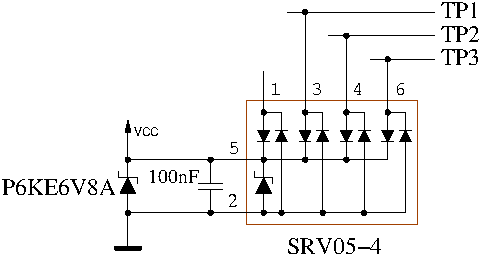
\includegraphics[width=.78\textwidth]{../FIG/diode_addon.pdf}
  \caption{с использованием диодов}
 \end{subfigure}
 \caption{Защита входов ATmega}
 \label{fig:relay_addon}
\end{figure}

Вы можете улучшить защиту, установив реле с тремя группами контактов, как показано на рисунке~\ref{fig:relay_um_addon}.
Разрядный ток ограничен резисторами, входы ATmega отключены в защищенном  режиме. 
Следует помнить, что тестер не защищён в режиме последовательных (циклических) измерений.

\begin{figure}[H]
\centering
 \begin{overpic}[width=.58\textwidth]{../FIG/relay_um_addon.pdf}
  \color{black}
  \put(78,42){\makebox(0,0)[lb]{\footnotesize VCC or Ubat}}  
  \put(78,32){\makebox(0,0)[lb]{\footnotesize depends on  U{\scriptsize реле}}}  
 \end{overpic}
\caption{Улучшенная защита с реле}
\label{fig:relay_um_addon}
\end{figure}

\subsection{Измерение стабилитронов с напряжением более 4 V}

Если UART не требуется, порт PC3 может использоваться в качестве аналогового входа для измерения внешнего напряжения. 
Напряжение может составить до \(50~V\) с дополнительным резистивным делителем 10:1. На рисунке ~\ref{fig:zener} 
представлена схема для измерения напряжение пробоя стабилитрона при низком уровне на порте PD7 ATmega. 
Тестер показывает внешнее напряжение, пока Вы держите кнопку \textbf{ TEST} нажатой. Ток, потребляемый от батареи питания, 
при этом возрастает, примерно, на \(40~mA\).

\begin{figure}[H]
\centering
  \begin{overpic}[width=.90\textwidth]{../FIG/zener_exp.pdf}
  \color{black}
  \put(5,20){\makebox(0,0)[rb]{\textcolor{red}{external}}}  
  \put(5,17){\makebox(0,0)[rb]{\textcolor{red}{Voltage}}}  
  \put(33,24){\makebox(0,0)[rb]{Can be placed on Tester board!}}
  \put(42,2){\makebox(0,0)[lb]{Should be placed separate!}}
 \end{overpic}
\caption{Схема для измерения параметров стабилитронов}
\label{fig:zener}
\end{figure}

Резистивный делитель 10:1 может быть использован для измерения внешних напряжений при выборе из
меню дополнительных функций в ATmega328. Присутствие DC-DC преобразователя для измерения стабилитронов
не мешает, так как кнопка не удерживается в нажатом состоянии и, соответственно, DC-DC преобразователь
обесточен. Таким образом, можно измерять напряжение постоянного тока до \(50~V\) только положительной 
полярности, обязательно соблюдая полярность.\\

\subsection{Генератор частоты}

Из меню дополнительных функций, при использовании ATmega, можно выбрать генератор частоты.
В настоящее время поддерживается выбор частот в диапазоне от \(1~Hz\) до \(2~MHz\). 
Выходной сигнал \(5~V\) через резистор \(680~\Omega\) выводится на тестовый контакт TP2.
В качестве сигнала GND, при этом, можно использовать GND DC-DC преобразователя или тестовый 
контакт TP1. Тестовый контакт TP3 подсоединен к GND через резистор \(680~\Omega\).
Конечно, Вы также можете использовать порт PB2 для подключения отдельной схемы усилителя-формирователя.
Но вход этой схемы не должен создавать большую нагрузку для порта ATmega.\\

\subsection{Измерение частоты}
\label{sec:frequency_counter}

Для использования дополнительной функции измерения частоты, потребуется незначительная 
доработка Тестера. Для измерения частоты используется порт PD4 (T0/PCINT20) ATmega. 
Этот же порт используется для подключения LCD-дисплея. В стандартном варианте к порту PD4 подключен 
сигнал LCD-RS, в варианте strip grid - сигнал LCD-D4. Для обоих сигналов порт PD4 может быть переключен 
на ввод, если в данный момент не требуется выводить информацию на LCD-дисплей.\\
 
Однако, лучше использовать дополнительную схему подключения, изображенную на рисунке~\ref{fig:FreqMes}.
Напряжение на выводе порта PD4 (LCD-RS или LCD-D4) должно быть установлено около \(2,4~V\) при отключенной 
ATmega или подстроено во время измерения частоты ATmega, чтобы получить лучшую чувствительность к входному 
сигналу. Во время регулировки LCD-дисплей должен быть установлен, потому что подтягивающие резисторы 
индикатора могут изменить установленное напряжение.

\begin{figure}[H]
\centering
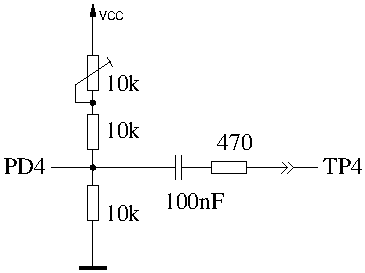
\includegraphics[width=.4\textwidth]{../FIG/Frequency_addon.pdf}
\caption{Дополнительная схема для измерения частоты}
\label{fig:FreqMes}
\end{figure}

\subsection{Использование поворотного энкодера}

Для более удобного доступа к Меню дополнительных функций для ATmega328, Вы можете дополнить схему, установив
инкрементальный энкодер с кнопкой.   
Рисунок~\ref{fig:RotExt} показывает схему подключения к тестеру с символьным LCD.
Все сигналы для подключения поворотного инкрементального энкодера доступны в разъеме 
подключения LCD. По этому, модернизация возможна для большинства существующих тестеров.
Во многих случаях графический LCD собран на переходной плате и подключен к контактам, предназначенным
для подключения символьного LCD. Таким образом, модернизация в этих случаях также возможна.    

\begin{figure}[H]
\centering
 \begin{overpic}[width=.30\textwidth]{../FIG/rotary_extension.pdf}
  \color{black}
%  \put(47,6){\makebox(0,0)[lb]{Taster}}    
 \end{overpic}
\caption{Схема подключения поворотного энкодера}
\label{fig:RotExt}
\end{figure}

На рисунке~\ref{fig:RotEnc} показана особенность работы двух типов поворотных инкрементальных 
энкодеров.
В версии 1 полная последовательность состояния переключателей происходит при повороте на два 
фиксированные положения. Количество полных циклов в два раза меньше чем количество фиксированных
положений за оборот энкодера.
В версии 2 при повороте на одно фиксированное положение генерируется полный цикл состояния контактов. 
В этом случае количество фиксированных положений соответствует количеству циклов за оборот энкодера.  
Иногда, в таких энкодерах, в каждом фиксированном положении состояние переключателей всегда 
одинаково.
\begin{figure}[H]
\centering
 \begin{overpic}[width=.87\textwidth]{../FIG/rotary_encoder.pdf}
  \color{black}
  \put(90,71.5){\makebox(0,0)[lb]{тумблер A}}
  \put(90,62){\makebox(0,0)[lb]{тумблер B}} 
  \put(90,29){\makebox(0,0)[lb]{тумблер A}}
  \put(90,19){\makebox(0,0)[lb]{тумблер B}}
  \put(6,6){\makebox(0,0)[rb]{\footnotesize состояние}}    
  \put(6,48.5){\makebox(0,0)[rb]{\footnotesize состояние}}    
  \multiput(23.5,53)(24.6,0){3}{\footnotesize стопор}
  \multiput(11,10)(12.3,0){6}{\footnotesize стопор}
  \put(52,43){\makebox(0,0)[cb]{{\large версия 2}}}
  \put(52,1){\makebox(0,0)[cb]{{\large версия 1}}}      
 \end{overpic}
 \caption{Особенности двух типов поворотных инкрементальных энкодеров}
 \label{fig:RotEnc}
\end{figure}
Рисунок~\ref{fig:RotBounce} показывает работу энкодера, который имеет не только \inquotes{дребезг} контактов
но и неустойчивое состояние переключателя в точке фиксации. Каждое изменение 
состояния переключателей определяется программой и сохраняется в циклический буфер.
Поэтому, последние три состояния переключателей можно проверить после каждого изменения состояния.
Для каждого цикла переключения состояний, в общей сложности четыре последовательности могут быть 
определены для каждого направления вращения.

Если за одну фиксированную позицию осуществляется один, полный, цикл состояний переключателей, то для правильного
подсчета достаточно контролировать состояние переключателя в одном канале (WITH\_ROTARY\_SWITCH=2 или 3).

Если для генерации полного цикла состояний переключателей требуется поворот на две фиксированные
позиции, как показано на рисунке~\ref{fig:RotBounce}, Вы должны контролировать последовательность
переключения в двух каналах (WITH\_ROTARY\_SWITCH=1).

Для энкодеров без фиксации, Вы можете выбрать любую чувствительность к углу поворота. Значение 
2 и 3 устанавливает низкую чувствительность, 1 среднюю чувствительность и 5 высокую чувствительность.

Подсчет импульсов (количество \inquotes{вверх}, количество \inquotes{вниз}) может быть обеспечен подбором 
определенного алгоритма, но, в то же время, может быть утрачен из-за неустойчивого состояния 
контактов переключателей в точке фиксации.
\begin{figure}[H]
\centering
 \begin{overpic}[width=.87\textwidth]{../FIG/rotary_bouncing.pdf}
  \color{black}
  \put(90,39){\makebox(0,0)[lb]{окошечко A}}
  \put(90,30){\makebox(0,0)[lb]{окошечко B}}
  \multiput(12,23)(28,0){3}{\footnotesize защелка}
  \put(7,20){\makebox(0,0)[rb]{состояние}}
  \put(5,12){\makebox(0,0)[lb]{Возможные состояния слева направо:}}      
 \end{overpic}
	\caption{Энкодер с \inquotes{дребезгом} контактов переключателей}
 \label{fig:RotBounce}
\end{figure}	
Если энкодер не доступен или не целесообразен из-за конструктивных соображений, вместо двух контактов энкодера, 
Вы можете подсоединить две независимые кнопки для перемещения \inquotes{Вверх} и \inquotes{Вниз}.
В этом случае значение опции WITH\_ROTARY\_SWITCH, для корректной работы программы, должно быть установлено 4.

\subsection{Подключение графического дисплея}

Большое спасибо Wolfgang Sch. за выполненную работу по поддержке прибором китайской версии дисплея с контроллером ST7565.
В настоящее время вы также можете подключить графический LCD (128x64 пикселей) с контроллером ST7565. 
Поскольку контроллер ST7565 подключается по последовательному интерфейсу, то только четыре сигнальных
линии используется. Два вывода порта D ATmega могут быть использованы для других задач.
ATmega процессор должен иметь, по крайней мере, \(32~kB\) флеш-памяти для поддержки графического дисплея.
ST7565 контроллер использует рабочее напряжение \(3,3~V\).
Поэтому требуется дополнительный стабилизатор \(3,3~V\).
Документация к контроллеру ST7565 не допускает прямого подключения логических 
сигналов уровня \(5~V\). Для согласования логических уровней сигналов \(5~V\) и \(3,3~V\) можно использовать
схему, приведенную на рисунке \ref{fig:ST7565lcd} с использованием 
микросхемы преобразователя уровней 74HC4050.
Вы можете попробовать применить вместо четырех элементов 74HC4050 четыре резистора, примерно \(2,7~k\Omega\).
Падение напряжения на резисторах предотвратит увеличение напряжения на входах графического контроллера больше чем
напряжение питания \(3,3~V\), а дополнительные диоды на входах графического контроллера не допустят попадания 
выходного сигнала \(5~V\) от ATmega.
Вы должны убедиться, что форма сигналов с резисторов могут быть правильно восприняты входами контроллера ST7565.
 
В любом случае, при применении элементов микросхемы 74HC4050 форма сигнала на входе графического контроллера 
точнее соответствует форме выходного сигнала с ATmega. 

\begin{figure}[H]
\centering
 \begin{overpic}[width=.814\textwidth]{../FIG/ST7565lcd.pdf}
  \color{black}
  \put(88,10){\makebox(0,0)[lb]{Background}}
  \put(88,7){\makebox(0,0)[lb]{LED}}
 \end{overpic}
\caption{Подключение графического дисплея с контроллером ST7565}
\label{fig:ST7565lcd}
\end{figure}

В таблице \ref{tab:spi-processor} показаны другие альтернативы подключения ATmega328 
или других микроконтроллеров по интерфейсу SPI (LCD\_INTERFACE\_MODE=4) или для трехпроводного
соединения (LCD\_INTERFACE\_MODE=3).
Различные типы подсоединений для одного типа процессора могут быть выбраны с помощью опции
в \lname{Makefile} STRIP\_GRID\_BOARD.
Назначение контактов разъема определено в файле \lname{config.h}.
Если Вам нужно иное подключение, Вы должны назначить новый номер кода для 
опции STRIP\_GRID\_BOARD и задать настройку подключения в файле \lname{config.h}.

\begin{table}[H]
  \begin{center}
    \begin{tabular}{| c || c | c | c | c | c | c | c |}
    \hline
 Контроллер  & m644  & m1280 & m1280  & m328 & m328 & m328 & m328 \\
STRIP\_GRID\_BOARD &       &   -   &   1    &  -   &  1   &  2   &  5   \\
Сигнал:     &       &       &        &      &      &      &     \\
    \hline
    \hline
  RES       &  PB4  & PA0   &  PA4   & PD0  & PD4  & PD0  & PD2 \\
    \hline
  EN, CLK   &  PB6  & PA2   &  PA2   & PD2  & PD2  & PD2  & PD3 \\
    \hline
  RS, D/C   &  PB5  & PA1   &  PA3   & PD1  & PD3  & PD3  & PD1 \\
    \hline
  B0, MOSI  &  PB7  & PA3   &  PA1   & PD3  & PD1  & PD1  & PD4 \\
    \hline
  CE, CS    &  PB3  & PA4   &  PA5   & PD5  & PD5  & PD5  & PD5 \\
    \hline
    \end{tabular}
  \end{center}
  \caption{Подключение по SPI для различных контроллеров}
  \label{tab:spi-processor}
\end{table}

Обычно ST7565 или SSD1306 контроллер подключается по 4-проводному SPI интерфейсу.
Но с контроллером SSD1306 Вы также можете подключить индикатор по интерфейсу I\textsuperscript{2}C использовав PD2 
как SDA и PD5 как SCL сигнал.
Сигналы SDA и SCL должны быть подтянуты резисторами около \(4,7~k\Omega\) к напряжению \(3,3~V\).
Пример подключения OLED дисплея показан на рисунке~\ref{fig:ssd1306i2c}.
Сигналы шины I\textsuperscript{2}C реализованы только путем переключения портов ATmega к \(0~V\).
Перед подключением подтягивающих резисторов к напряжению \(5~V\), Вы должны убедиться, что Ваш контроллер
допускает уровень сигнала \(5~V\). Обычно входы контроллера дисплея защищены диодами, которые понижают уровень 
сигнала до \(3,3~V\). 
Вы должны убедиться, что в ATmega записана программа с поддержкой интерфейса I\textsuperscript{2}C до того,
как дисплей будет подсоединен. Если Вы записали в контроллер микропрограмму с поддержкой другого интерфейса,
то на выводах ATmega могут присутствовать сигналы с уровнем \(5~V\).

Так, как я обнаружил влияние на результаты теста модуля OLED через шину \(VCC\), рекомендую
установить дополнительную развязку из последовательного резистора \(68~\Omega\) и разделительного конденсатора \(10~\mu F\). 
Вместо \(68~\Omega\) резистора можно также использовать индуктивность \(1~mH\).
Без дополнительного фильтра мой тестер с дисплеем OLED определял остаточные токи в коллекторах биполярных транзисторов.

Также нужно проверить расположение выводов Вашего OLED дисплея. Некоторые модули имеют отличие в расположении \(GND\) и \(VCC\).   
 
\begin{figure}[H]
\centering
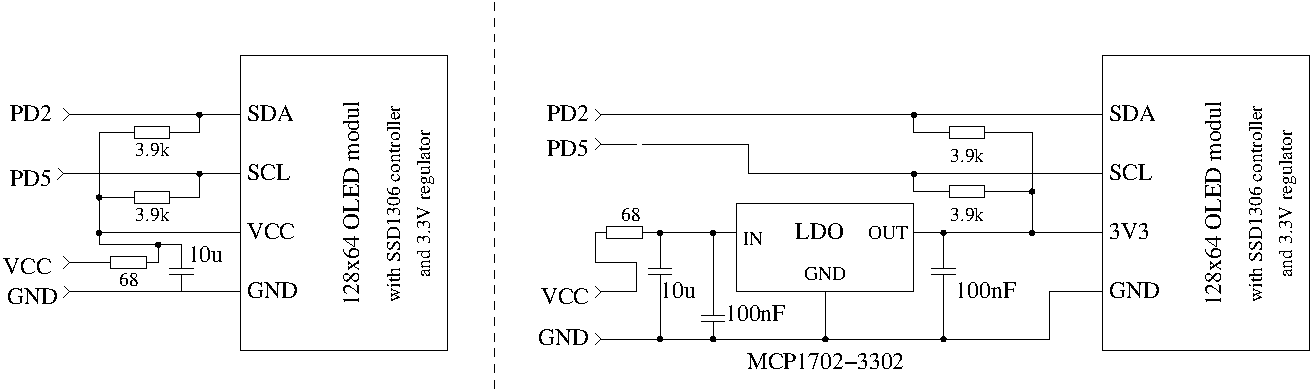
\includegraphics[width=.814\textwidth]{../FIG/SSD1306_I2C.pdf}
\caption{Подключение графического OLED дисплея с I\textsuperscript{2}C интерфейсом}
\label{fig:ssd1306i2c}
\end{figure}

Для подключения к контроллерам серии ATmega644 вместо портов PB3 (SCL) и PB4 (SDA) используются порты PD5 и PD2.
Для микроконтроллеров серии ATmega1280 используются контакты PA5 (SCL) и PA4 (SDA).
Для замены символьного дисплея на графический можно использовать переходную печатную плату-адаптер с разъемом
аналогичным символьному LCD, так как все сигналы и питание на нем доступны.

Намного проще подключить дисплей с контроллером ST7920, потому что контроллер поддерживает напряжение питания \(5~V\).
Дисплей должен поддерживать режим 128x64 точек.
Модуль дисплея с контроллером ST7920 может быть подключен по 4-bit параллельному интерфейсу или по специальному,
последовательному интерфейсу, согласно рисунка \ref{fig:ST7920lcd}.

\begin{figure}[H]
\centering
 \begin{overpic}[width=.698\textwidth]{../FIG/ST7920interface.pdf}
  \color{black}
  \put(20,1){\makebox(0,0)[cb]{serial mode}}  
  \put(80,1){\makebox(0,0)[cb]{4-bit parallel mode}}   
 \end{overpic}
\caption{Подключение индикатора с контроллером ST7920}
\label{fig:ST7920lcd}
\end{figure}

Для двух типов подключения индикатора с контроллером ST7920 в \lname{Makefile} должна быть установлена опция 
\inquotes{WITH\_LCD\_ST7565 = 7920}. Кроме того, при подключении по последовательному интерфейсу, 
надо установить и опцию \inquotes{CFLAGS += -DLCD\_INTERFACE\_MODE=5}.

В таблице~\ref{tab:ser-processor} показано подключение различных микроконтроллеров по
последовательному интерфейсу с опциями INTERFACE\_MODE 5 (ST7920) и 7 (SSD1803).

\begin{table}[H]
  \begin{center}
    \begin{tabular}{| c || c | c | c | c |}
    \hline
 Контроллер  & m644  & m644 & m1280  & m328 \\
STRIP\_GRID\_BOARD &   -   &   1   &        &     \\
Сигнал:     &       &       &        &         \\
    \hline
    \hline
  EN        &  PB3  & PB6   &  PA5   & PD5     \\
    \hline
  B0, R/W   &  PB4  & PB7   &  PA4   & PD2      \\
    \hline
  RESET     &  PB2  & PB4   &  PA0   & PD0      \\
    \hline
    \end{tabular}
  \end{center}
  \caption{Порты для последовательного подключения различных контроллеров}
  \label{tab:ser-processor}
\end{table}

Так же как и в случае применения других графических индикаторов, для дисплея с контроллером ST7920,
опциями LCD\_ST7565\_H\_FLIP и LCD\_ST7565\_V\_FLIP можно изменить ориентацию выводимого изображения.

Особым случаем является подключение дисплеев с контроллером NT7108 (KS0108, S6B0108). Поскольку эти дисплеи 
используют только параллельный 8-битный интерфейс, необходимо применение последовательно - параллельного 
преобразователя интерфейсов. Простейший способ -- использование микросхемы 74HCT164 или 74HCT595.
Вариант такого подключения показан на рисунке \ref{fig:NT7108lcd}.

\begin{figure}[H]
  \begin{subfigure}[b]{.5\textwidth}
    \centering
    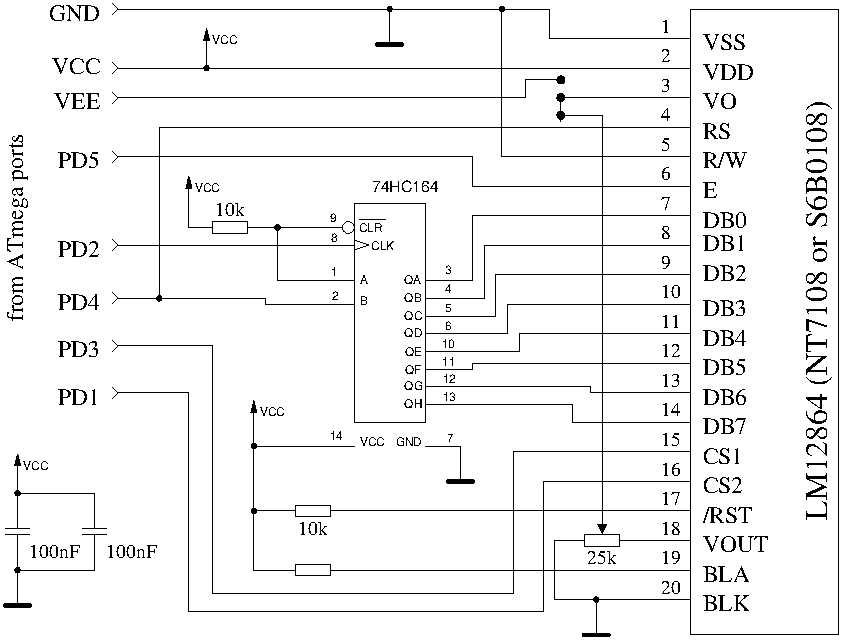
\includegraphics[width=.9\textwidth]{../FIG/ST7108serial164.pdf}
    \caption{с использованием 74HCT164}
  \end{subfigure}
  ~
  \begin{subfigure}[b]{.5\textwidth}
    \centering
    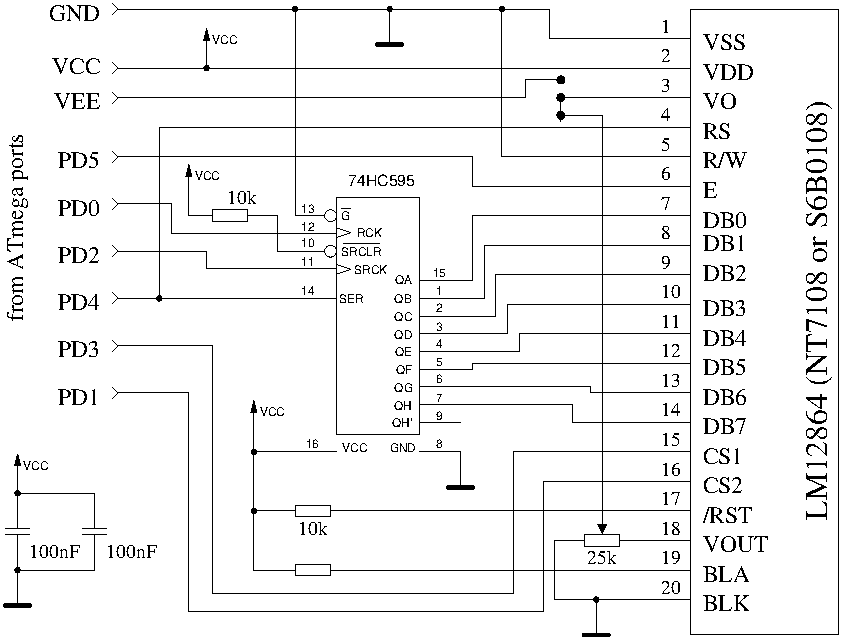
\includegraphics[width=.9\textwidth]{../FIG/ST7108serial595.pdf}
    \caption{с использованием 74HCT595}
  \end{subfigure}
  \caption{Подключение графического дисплея с NT7108 контроллером}
  \label{fig:NT7108lcd}
\end{figure}

Так как некоторые модули LCD различаются по расположению выводов, перед подключением Вы должны проверить цоколёвку 
Вашего дисплея. 
Некоторые различия в расположении выводов для серии LCD ABG128064 приведены в таблице~\ref{tab:NT7108types}.

\begin{table}[H]
  \begin{center}
    \begin{tabular}{| c || c | c | c | c |}
    \hline
           & 128064H  &  128064G  & 128064C  & 128064B \\
    Сигнал &         &          &         &         \\
    \hline
    \hline
  VDD (5V) &   1     &  2       &   4     & 2       \\
    \hline
  VSS (GND) &   2     &  1       &   3     & 1       \\
    \hline
 VO (Drive) &   3     &  3       &  (5)    & 3       \\
    \hline
  DB0-DB3   &   4-7   &  7-10    &   9-12  & 7-10    \\
    \hline
  DB4-DB7   &   8-11  &  11-14   &   13-16 & 11-14   \\
    \hline
  CS1       &   12    &  15      &   1     & 15      \\
  CS2       &   13    &  16      &   2     & 16      \\
    \hline
  Reset     &   14    &  17      &   -     & 17      \\
    \hline
  R/W       &   15    &  5       &   7     & 5       \\
    \hline
  RS        &   16    &  4       &   6     & 4       \\
    \hline
  E         &   17    &  6       &   8     & 6       \\
    \hline
  VEE       &   18    &  18      &   -     & 18      \\
    \hline
  LEDA      &   19    &  19      &   17    & (19)      \\
  LEDK      &   20    &  20      &   18    & -      \\
    \hline
    \end{tabular}
  \end{center}
  \caption{Различие в цоколёвке NT7108 модулей}
  \label{tab:NT7108types}
\end{table}

В таблице \ref{tab:7108-processor} показано подключение по последовательному интерфейсу индикаторов 
NT7108 к различным микроконтроллерам.
\begin{table}[H]
  \begin{center}
    \begin{tabular}{| c || c | c | c |}
    \hline
Контроллер  & m644  &  m1280  & m328 \\
Сигнал:     &       &        &         \\
    \hline
    \hline
  EN        &  PB3  &  PA5   & PD5     \\
    \hline
  RS        &  PB2  &  PA4   & PD4      \\
  B0        &  PB2  &  PA4   & PD4      \\
    \hline
  CS1       &  PB7  &  PA3   & PD3      \\
    \hline
  CS2       &  PB5  &  PA1   & PD1      \\
    \hline
  CLK       &  PB6  &  PA2   & PD2      \\
    \hline
  PCLK      &  PB4  &  PA0   & PD0      \\
    \hline
    \end{tabular}
  \end{center}
  \caption{Подключение индикаторов с NT7108 по последовательному интерфейсу}
  \label{tab:7108-processor}
\end{table}

Вы также можете использовать дисплей с контроллером PCF8814, который обычно используется, 
например, в Nokia 1100. 
Вы должны проверить, какой интерфейс контроллера используется в Вашем модуле дисплея.
Контроллер PCF8814 может поддерживать SPI-интерфейс 3-х проводной или 4-х проводной, 
I\textsuperscript{2}C-интерфейс и специальный 3-х проводной, который ждёт сигнал 
данные/команда в качестве первого бита в 8 битных данных.
Потому, что дисплей поддерживает только 96х65 пикселей, большие иконки для транзисторов не используются 
с этим контроллером. Вывод результатов похож на вывод для символьных дисплее. 
Как и большинство графических дисплеев, этот контроллер работает с \(3,3~V\). 
Поэтому требуется преобразователь уровней логических сигналов для \(5~V\) выходов ATmega.
Для SPI интерфейса и 3-х проводного интерфейса Вы можете использовать опцию в \lname{Makefile}
LCD\_SPI\_OPEN\_COL (\inquotes{открытый коллектор} портов ATmega).
Вы должны использовать \inquotes{Pull-Up} резисторы или не устанавливать 
опцию PULLUP\_DISABLE в \lname{Makefile}.  
В настоящее время с контроллером PCF8814 протестирован только 3-х проводной интерфейс.

\begin{table}[H]
  \begin{center}
    \begin{tabular}{| c || c | c | c | c |}
    \hline
     Порт  &  PCF8814    & PCF8814        & PCF8814     & Дополнительная \\
           &    SPI      & 3-х проводной  & I\textsuperscript{2}C  & функция \\
    \hline
    \hline
    PD0    &   LCD-RESet  & LCD-RESset       &            & \\
    \hline
    PD1    &   LCD-D/C   & LCD-SCE        &             & Энкодер 2 \\
    \hline
    PD2    &   LCD-SCLK  & LCD-SCLK       &  LCD-SDIN   & \\
    \hline
    PD3    &   LCD-SDIN  & LCD-SDIN       &             & Энкодер 1 \\
    \hline
    PD4    &             &                &             & Внешняя частота \\
    \hline
    PD5    &             & LCD-EN         &   LCD-SCLK  & \\
    \hline
    \end{tabular}
  \end{center}
  \caption{Назначение контактов для различных типов интерфейсов контроллера PCF8814}
  \label{tab:PCF8814-con}
\end{table}

Исходный код для поддержки контроллера PCF8812 с 102x65 пикселей также реализован, 
но, пока, не тестировался.

\subsection{Подключение графического цветного дисплея}

В предложениях китайских продавцов встречаются дешевые модули цветных дисплеев с интерфейсом SPI.
На рисунке \ref{fig:Color_both} показан вид сзади двух поддерживаемых дисплеев с 128x128 и 
128x160 пикселей.
Размер модулей очень мал, поэтому текст и символы очень мелкие.
Но, в целом, внешний вид четкий и ясный.

\begin{figure}[H]
\centering
\includegraphics[width=.46\textwidth]{../PNG/Color_ILI9163_ST7735.jpg}
\caption{Вид сзади двух цветных LCD}
\label{fig:Color_both}
\end{figure}

Модуль 128x128 пикселей использует контроллер ILI9163.
Модуль 128x160 пикселей использует контроллер очень близкий к ST7735 контроллеру.
Модули тестировались с платой адаптера, которая соединяет сигналы SPI и питание выводов для 
нормального отображения символов. Адаптация выходных уровней \(5~V\) сигналов ATmega к уровню \(3,3~V\) 
сигналов входов контроллера обеспечивается последовательными \(10 k\Omega\) резисторами.
Наличие подсветки (LED) обязательно, т.к. без нее выводимую информацию невозможно прочесть.
Из-за высокого разрешения по вертикали можно отобразить несколько текстовых строк в этих модулях.
Для дисплея 128x128 пикселей можно отобразить 8 строк текста шрифтом 12x8,
для дисплея 128x160 пикселей получим 10 строк текста.
На рисунке \ref{fig:Color_PNP} Вы можете видеть результат измерения германиевого транзистора
на дисплее 128x128 пикселей.

\begin{figure}[H]
\centering
\includegraphics[width=.46\textwidth]{../PNG/Color_PNP_ILI9163.jpg}
\caption{Измерение биполярного PNP транзистора}
\label{fig:Color_PNP}
\end{figure}

Цветность модулей в настоящее время не используется.
Цвет фона и цвет отображаемых элементов можно изменить в файле lcd\_defines.h или
в \lname{Makefile}.
Контроллер использует программное 16-битное управление цветностью. Цвет отображаемой информации может 
быть изменен параметром LCD\_FG\_COLOR, а цвет подсветки параметром LCD\_BG\_COLOR .



\section{Указания по сборке Тестера }

В Тестере может использоваться LCD-дисплей 2x16, программно совместимый с HD44780 или ST7036. Вы должны учитывать ток, 
необходимый для подсветки, некоторым LCD-дисплеям нужен ток ниже, чем другим. Я пытался применить OLED-дисплей, но он 
стал причиной помех при измерениях для ATmega, и я его \textbf{ не} рекомендую. Также использование OLED-дисплея вызвало 
проблему загрузки специального символа для отображения резистора.\\

Чтобы получить максимальную точность измерения, резисторы R1 - R6 \(680~\Omega\) и
\(470~k\Omega\) должны быть точными (0,1\%). В Тестере могут использоваться ATmega8, ATmega168 и ATmega328. Для 
возможности использовать все функции, рекомендуется установить ATmega328.\\
 
Сначала Вы должны собрать все элементы Тестера на печатной плате без микроконтроллера. В качестве IC2 рекомендуется 
использовать стабилизатор с малым падением напряжения MCP1702-5002, потому что он потребляет всего  \(2~\mu A\) и может 
выдавать \(5~V\) при входном напряжение всего \(5,4~V\). Но он несовместим по выводам с известным 78L05 в корпусе TO92 .\\

После проверки правильности монтажа, необходимо подсоединить батарею или источник питание к плате без LCD-дисплея и 
микроконтроллера. При нажатой кнопке \textbf{ TEST} должно присутствовать напряжение \(5~V\) на выводах питания 
микроконтроллера и LCD дисплея. Если отпустить кнопку \textbf{ TEST}, напряжение должно исчезнуть. Если  напряжения 
в норме, то необходимо отключить питание, \textbf{ правильно} вставить микроконтроллер и подключить LCD-дисплей. 
Перед подключением LCD дисплея необходимо 
внимательно проверить правильность соединения выводов питания LCD дисплея (т.к. на некоторых LCD дисплеях они 
подключены наоборот) с GND и VCC платы Тестера!\\
 
Если Вы уверены, что все в порядке, можно подсоединить питание. Если Вы уже запрограммировали ATmega, то можете 
кратковременно нажать кнопку \textbf{ TEST}. При кратковременном нажатии кнопки \textbf{ TEST} светодиод LED1 и подсветка 
LCD-дисплея должны включиться. 
Если Вы отпускаете кнопку \textbf{ TEST}, светодиод LED1 не должен гаснуть как минимум несколько секунд 
(зависит от установленных параметров при компилляции программного обеспечения). 
Заметьте, что программное обеспечение для микроконтроллера должно быть для используемого типа микроконтроллера. Программа для ATmega8 не работает на ATmega168!


\section{Доработки для версий Тестера Markus F.}
\label{sec:change_markus}
\begin{description}

\item[Контроль напряжения.]
Проблема проявляется следующим образом: Тестер немедленно отключается при каждом включении. Причиной может стать 
установка фьюзов (\lname{Makefile}) контроля за понижением напряжения питания ATmega на \(4,3~V\). Происходит это следующим 
образом: порт PD6 пытается зарядить конденсатор C2 \(100~nF\) до уровня VCC, что вызывает провал напряжения 
VCC (\(5~V\)). Для решения проблемы конденсатор C2 может быть уменьшен до \textless~\(10~nF\). Если возможно, 
то включить последовательно в цепь PD6  резистор сопротивлением более \textgreater~\(220~\Omega\).
\item[Улучшение питания схемы.]
Если Тестер запускается при нажатии на кнопку \textbf{ TEST}, но ключ сразу же отпускается, то часто причина этой проблемы 
в питании. Проблема порождена большим током подсветки LCD-дисплея. Резистор R7 к базе P-N-P-транзистора T3 был 
величиной \(27~k\Omega\), 
чтобы уменьшить потребление энергии. Чтобы улучшить переключение при  более низком напряжении батареи или при низком 
коэффициенте усиления P-N-P транзистора T3, необходимо уменьшить сопротивление до \(3,3~k\Omega\).
\item[Дополнительный подтягивающий резистор порта PD7.]
Отсутствие подтягивающего резистора, после короткого времени, работа заканчивается  выключением Тестера с сообщением 
\inquotes{Timeout}. Программное обеспечение формируется с опцией PULLUP\_DISABLE, т. е. все внутренние подтягивающие резисторы 
отключены. По этой причине напряжение порта PD7 не определено, если уровень не переключен кнопкой \textbf{ TEST} или 
транзистором T2 к GND. Внешний резистор сопротивлением \(27~k\Omega\) к VCC решает эту проблему.
\item[Конденсатор C1 в AREF.]
Многие используют на контакте AREF конденсатор на \(100~nF\) так же, как и Markus F. Пока не было необходимости менять 
опорное напряжение АЦП - это было хорошим решением. Программное обеспечение для ATmega168 и ATmega328 использует 
автоматический выбор внутреннего опорного напряжения АЦП \(1,1~V\), если входное напряжение ниже \(1~V\). Это позволяет 
улучшить разрешение АЦП при небольших входных напряжениях. К сожалению, переключение опорного напряжения от \(5~V\) до 
\(1,1~V\) происходит очень медленно. По этой причине нужно учитывать дополнительное время ожидания \(10~ms\). 
При уменьшении величины конденсатора до \(1~nF\), это время может быть существенно уменьшено. Я не заметил ухудшения 
качества измерения при этом изменении. Даже с удалённым конденсатором нет существенного изменения результатов 
измерения. Если Вы предпочитаете оставить конденсатор на \(100~nF\), то можете отключить опцию NO\_AREF\_CAP
в \lname{Makefile}, для активации увеличения времени ожидания в программе.
\item[Установка кварца на \(8~MHz\).]
Вы можете установить кварц на \(8~MHz\) с задней стороны печатной платы непосредственно к портам PB6 и PB7 
(выводы 9 и 10). Моя собственная доработка была сделана без конденсаторов \(22~pF\) и работала хорошо со всеми 
проверенными ATmega. Вы так же можете, выбрав фьюзы, использовать внутренний генератор на \(8~MHz\) для получения 
лучшего разрешения по времени при стабильных измерениях величины ёмкостей.
\item[Сглаживание питающего напряжения.]
В оригинальной схеме Markus F. применен только один конденсатор \(100~nF\) по напряжению VCC. Это не дает приемлемую 
фильтрацию. Вы должны, по крайней мере, использовать конденсаторы ёмкостью \(100~nF\) около выводов питания ATmega и 
возле выводов входа и выхода стабилизатора напряжения. Дополнительные конденсаторы \(10~\mu F\)
(электролитические или танталовые) на входе и выходе стабилизатора напряжения повышают устойчивость напряжения. 
Танталовый SMD конденсатор  \(10~\mu F\) легче использовать со стороны печатных дорожек, и он имеет обычно более 
низкое значение ESR.
\item[Выбор микроконтроллера ATmega.]
Для основных функций Тестера возможно использование ATmega8, Flash память в ней используется практически на 100\%.
АТmega168 или АТmega328 совместимы по выводам с ATmega8, я могу рекомендовать замену. 
При использовании ATmega168 или АТmega328 Вы получаете следующие преимущества: 
\begin{itemize} \setlength{\itemsep}{-1.5em}
 \item Самопроверка с автоматической калибровкой.\\
 \item Улучшение качества измерения с автоматическим переключением масштаба АЦП.\\
 \item Измерение индуктивностей  при сопротивлении ниже \(2100~\Omega\).\\
 \item Измерение величины ESR конденсаторов с ёмкостью выше \(20~nF\).\\
 \item Измерение резисторов ниже \(10~\Omega\) с разрешением \(0,01~\Omega\).\\
 \item Использование порта PC3 в качестве последовательного выхода или аналогового входа для измерения внешнего напряжения.\\
\end{itemize}
\item[Отсутствующие прецизионное опорное напряжение.]
Программное обеспечение должно обнаружить недостающие элементы опорного напряжения на выводе PC4. В этом случае при 
		включении питания во второй строке LCD-дисплея должно появиться сообщение \inquotes{No VCC = x.xV}. Если это сообщение 
появляется при установленном ИОН, Вы должны подключить резистор \(2,2~k\Omega\) между выводом PC4 и VCC.

\end{description}

\section{Расширенная схема с ATmega644 или ATmega1284}

Расширенная схема для контроллеров ATmega644/1284 разработана совместно с Nick L. из Украины.
Схема \ref{fig:t644tester} позволяет расширить диапазон измеряемых частот, а также содержит схему 
тестирования кварцев. 
Хотя расширенная схема почти идентична схеме на рисунке \ref{fig:ttester}, 
назначение портов несколько отличается.
Поворотный энкодер на схеме \ref{fig:RotExt} должен быть подключен к PB5 и PB7 (вместо PD1 и PD3).
Оба сигнала, а также VCC и GND доступны на разъеме программирования ISP. Таким образом, подключение
поворотного энкодера не должно вызвать затруднений.
Делитель 16:1 в 74HC4060 всегда используется для частот выше \(2~MHz\). 
Он также может быть использован для частот от \(24~kHz\) до \(400~kHz\) для повышения точности
измерения частоты с помощью подсчета периода.
Для коммутации переключений (делитель частоты и кварцевый генератор) используется 
аналоговый переключатель 74HC4052.
Таблица \ref{tab:mega644-display} показывает варианты подключения дисплея к портам 
ATmega324/644/1284.
Подключение индикатора с использованием интерфейса I\textsuperscript{2}C возможно только для индикаторов с 
контроллером SSD1306.
Сигналы интерфейса I\textsuperscript{2}C требуют установки подтягивающих резисторов \(4,7k\Omega\) к напряжению \(3,3~V\).
Сигналы шины I\textsuperscript{2}C реализованы только путем переключения портов ATmega к \(0~V\).

\begin{figure}[H]
\centering
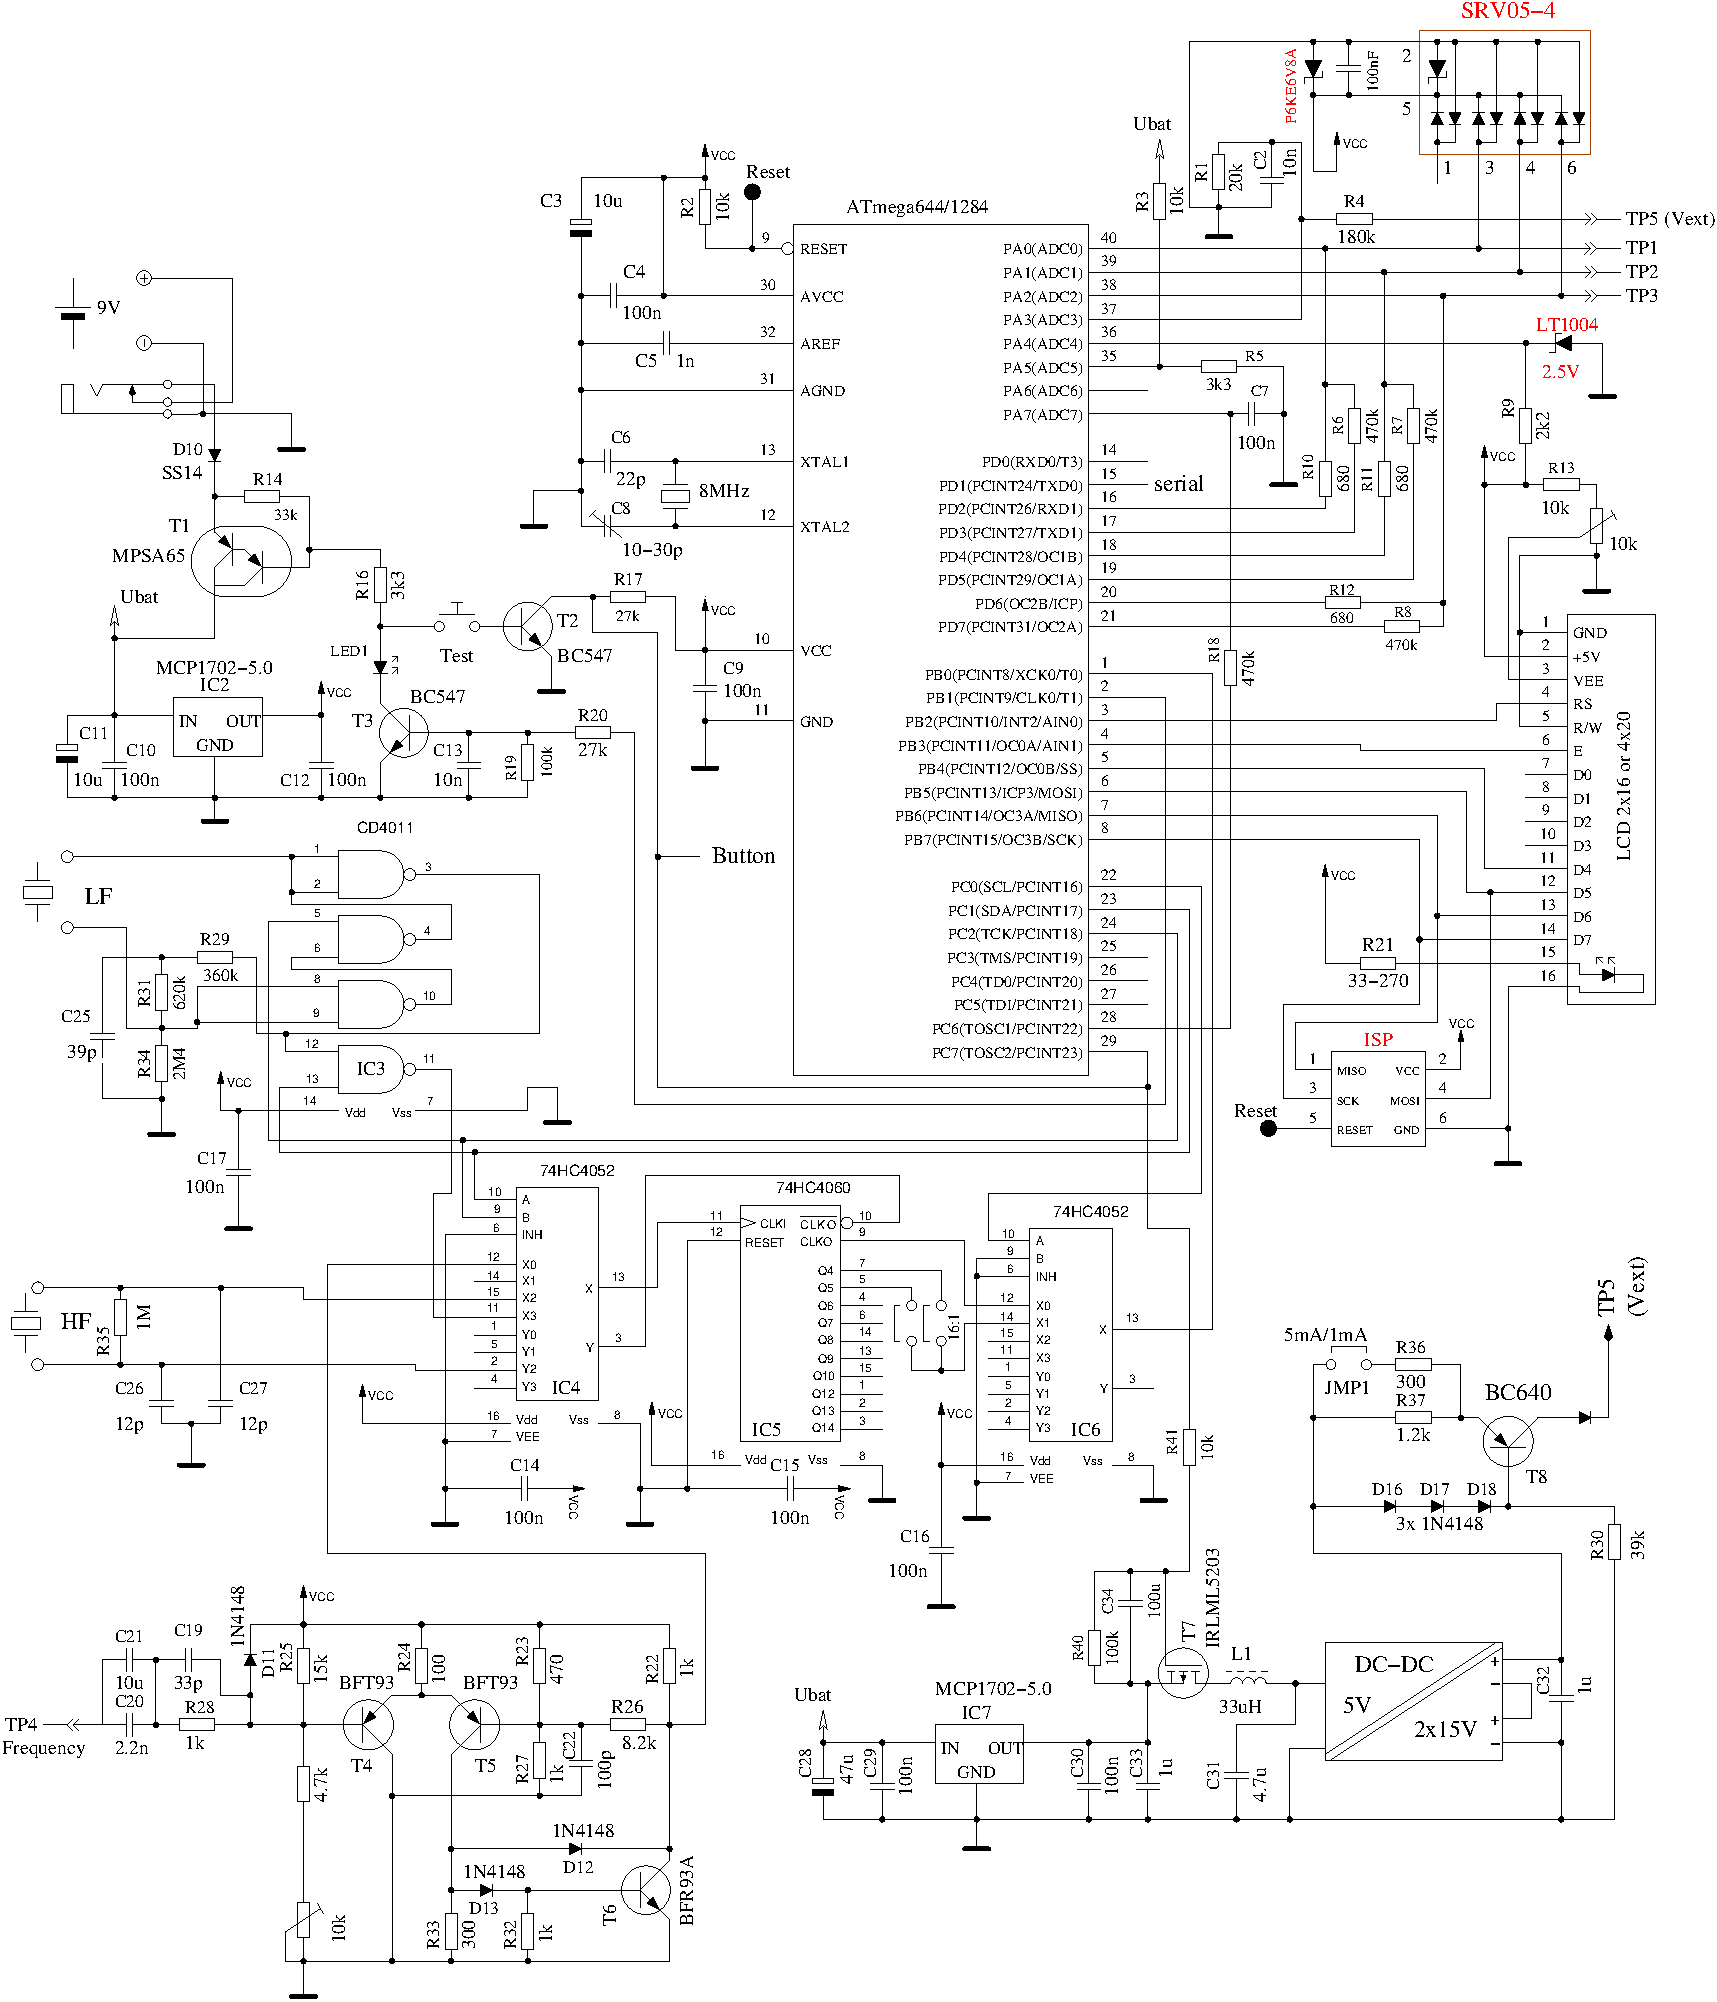
\includegraphics[width=1.\textwidth]{../FIG/t644tester.pdf}
\caption{Расширенная схема Транзистор Тестера с ATmega644}
\label{fig:t644tester}
\end{figure}

\begin{table}[H]
  \begin{center}
    \begin{tabular}{| c || c | c | c | c |}
    \hline
      Порт & Символьный & Графический LCD & Графический LCD & Дополнительные\\
	   &     LCD    &   SPI 4-wire &   I\textsuperscript{2}C      &  функции \\
    \hline
    \hline
    PB2    &  LCD-RS         &            &          &       \\
    \hline                                              
    PB3    &  LCD-E          &  (LCD-CE)  &  LCD-SCL &       \\
    \hline                                              
    PB4    &  LCD-D4         &  LCD-REST  &  LCD-SDA &       \\
    \hline                                              
    PB5    &  LCD-D5         &  LCD-RS    &          & ISP-MOSI \\
           &                 &            &          & поворотный энкодер 2 \\
    \hline                                              
    PB6    &  LCD-D6         &  LCD-SCLK  &          & ISP-MISO \\
    \hline                                            
    PB7    &  LCD-D7         &  LCD-SI    &          & ISP-SCK  \\
           &                 &            &          & поворотный энкодер 1 \\
    \hline
    \end{tabular}
  \end{center}
  \caption{Подключения дисплеев к портам ATmega324/644/1284}
  \label{tab:mega644-display}
\end{table}

Вы также можете подключить дисплей с контроллером NT7108 (KS0108, S6B0108) к тестеру, собранному на ATmega644 или ATmega1284
используя небольшую схему подключения показанную на рисунке~\ref{fig:NT7108lcd_644}.
Вы также должны учитывать различие в назначении контактов дисплейных модулей с контроллерами NT7108, 
как показано в таблице~\ref{tab:NT7108types} на странице~\pageref{tab:NT7108types}.

\begin{figure}[H]
  \begin{subfigure}[b]{.5\textwidth}
    \centering
    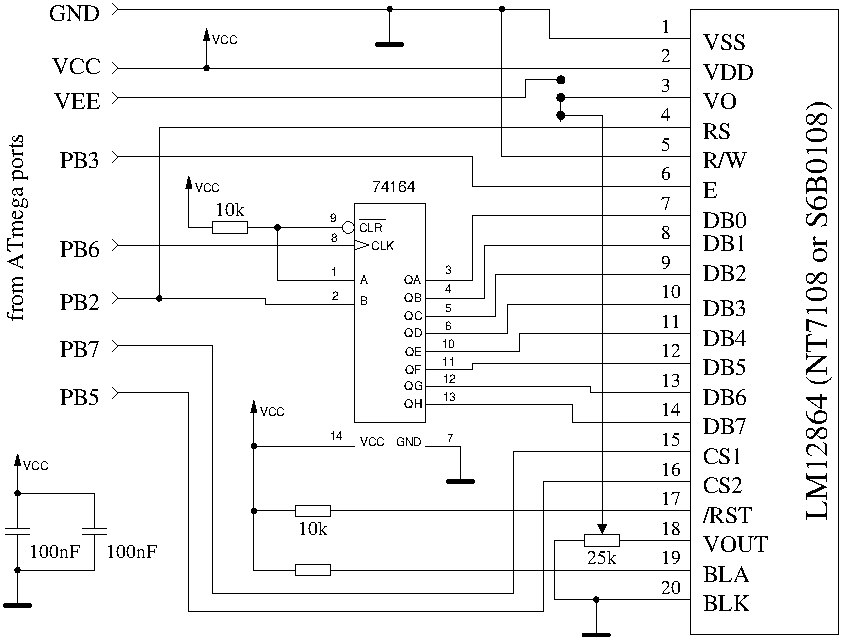
\includegraphics[width=.88\textwidth]{../FIG/ST7108serial164_644.pdf}
    \caption{при использовании 74HCT164}
  \end{subfigure}
  ~
  \begin{subfigure}[b]{.5\textwidth}
    \centering
    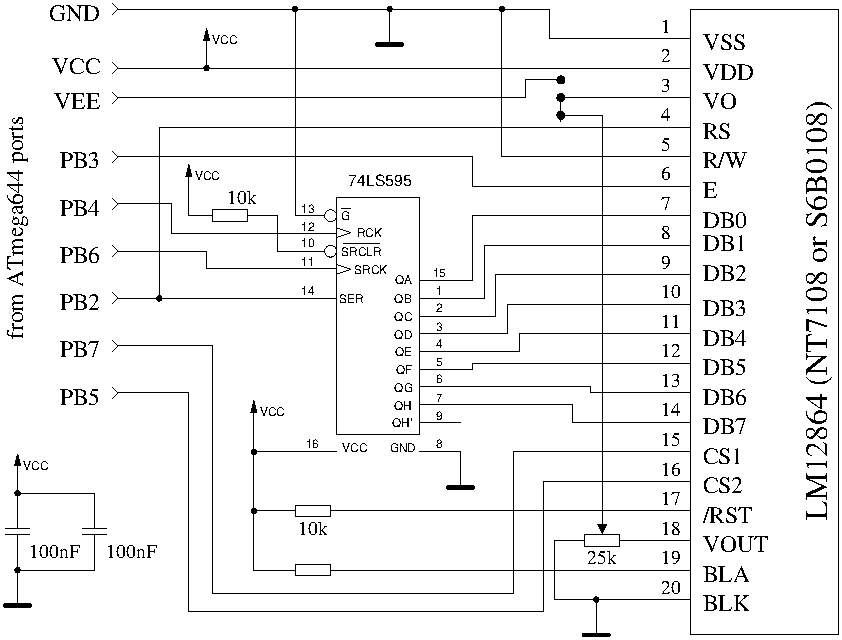
\includegraphics[width=.88\textwidth]{../FIG/ST7108serial595_644.pdf}
    \caption{при использовании 74HCT595}
  \end{subfigure}
  \caption{Подключение дисплея с контроллером NT7108 к ATmega644/1284}
  \label{fig:NT7108lcd_644}
\end{figure}

\section{Схема с использованием ATmega1280 или Arduino Mega}

Тестер может быть создан с использованием микроконтроллера ATmega1280 
или ATmega2560, а также построен на базе Arduino Mega.
Схема показана на рисунке~\ref{fig:t1280tester}.
Назначения контактов Arduino для подключения дисплея указаны зеленым цветом.
Компоненты, показанные красным цветом, не обязательны для правильной работы Тестера.
Контроллер ATmega2560 имеет большое количество портов, но только один порт
имеет функции, необходимые для обеих методик измерения частоты.
Порт должен быть одновременно таймером/счетчиком для подсчета внешних импульсов и
поддерживать внешнее прерывание при изменении уровня сигнала.
Этими функциями обладает только один порт PE6 (T3/INT6).
На остальных портах таймеров/счетчиков PD7 (T0), PD6 (T1), PH7 (T4) и PL2 (T5) отсутствует
внешнее прерывание.
К сожалению, порт PE6 не подключен к ленточному гнезду Arduino. 
Порт PE5 (вывод~7) подключен к контакту 3 разъема ШИМ и перемычкой 
может быть соединен с портом PE6 (вывод~8) ATmega2560.
Выходной сигнал генератора частоты можно получить на порту PB6 (OC1B).
Это порт подключен к контакту 12 разъема ШИМ.
ISP-разъем не требуется, так как программа может быть установлена при помощи  
загрузчика USB Arduino Mega. С использованием загрузчика есть небольшая задержка 
запуска программы.

\begin{figure}[H]
\centering
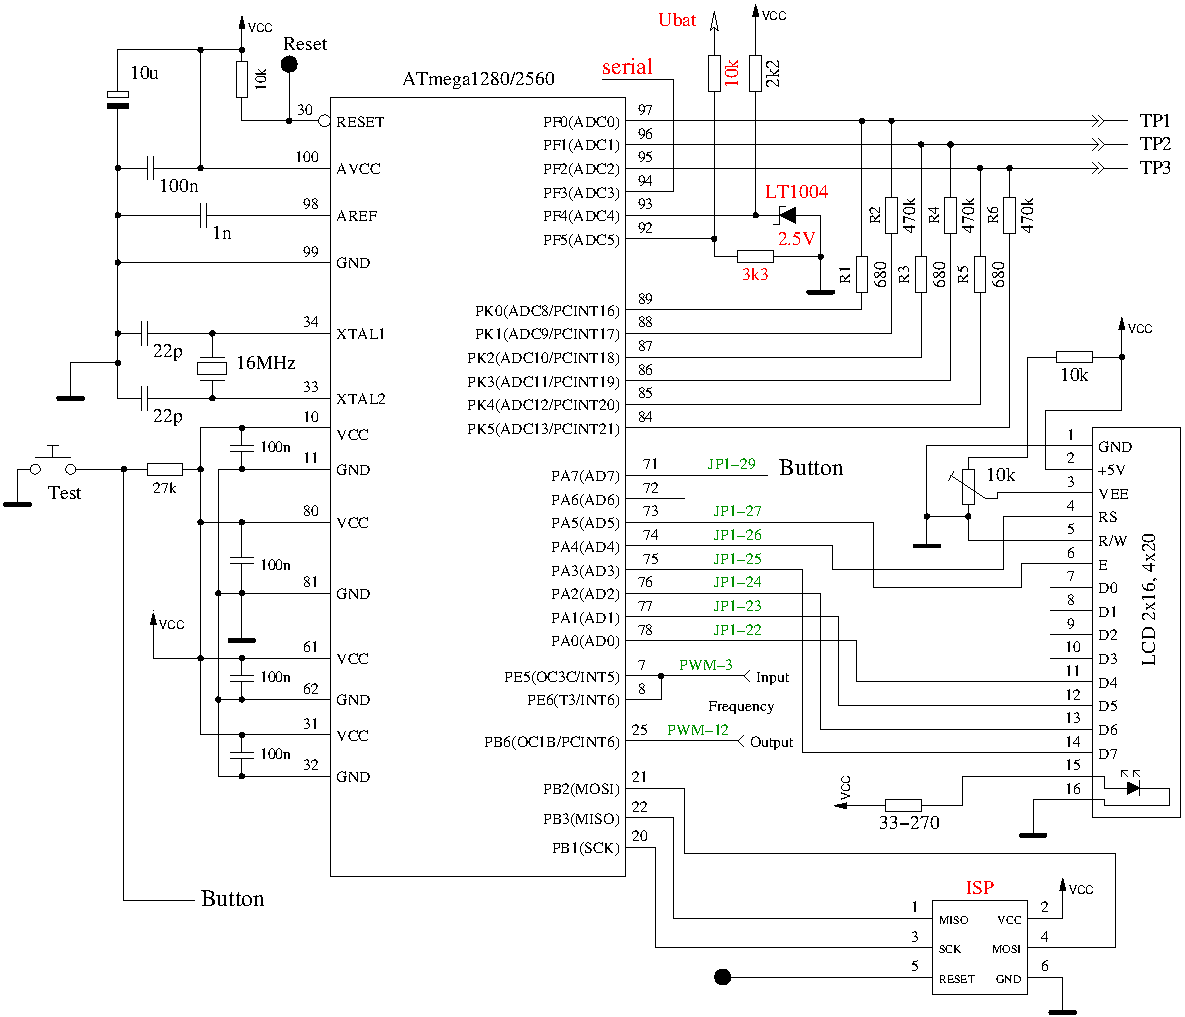
\includegraphics[width=1.\textwidth]{../FIG/t1280tester.pdf}
\caption{Схема Тестера с использованием ATmega1280, ATmega2560 или Arduino Mega}
\label{fig:t1280tester}
\end{figure}

Конечно, Вы можете подключить все поддерживаемые дисплеи и к ATmega1280 или ATmega2560
в соответствии с таблицей~\ref{tab:display-1280}.

\begin{table}[H]
  \begin{center}
    \begin{tabular}{| c || c | c | c | c | c | c |}
    \hline
      Порт & Символь-  &  ST7565     & ST7920       & NT7108       & SSD1306     & Дополнительные \\
           & ный LCD   &    SPI      & serial       & serial       & I\textsuperscript{2}C & функции \\
    \hline
    \hline
    PA0    &  LCD-D4   &   LCD-REST  &  LCD-RESET   & HC595-RCK      &             & \\
    \hline
    PA1    &  LCD-D5   &   LCD-RS    &              & LCD-CS2        &             & 2 канал энкодера \\
    \hline
    PA2    &  LCD-D6   &   LCD-SCLK  &              & HC164-CLK      &             & \\
    \hline
    PA3    &  LCD-D7   &   LCD-SI    &              & LCD-CS1        &             & 1 канал энкодера \\
    \hline
    PA4    &  LCD-RS   &             &   LCD-B0     & LCD-RS         &   LCD-SDA   & \\
           &           &             &              & HC164-SER      &             & \\
    \hline
    PA5    &  LCD-E    &   (LCD-CE)  &   LCD-EN     & LCD-EN         &   LCD--SCL  & \\
    \hline
    PA7    &  кнопка   &             &              &                &             & \\
    \hline
    \end{tabular}
  \end{center}
  \caption{Подключение различных дисплеев к ATmega1280/2560}
  \label{tab:display-1280}
\end{table}
\section{Китайские клоны с символьным дисплеем}
По имеющейся у меня информации, Тестер с символьным индикатором выпускают в Китае в двух версиях.
Первая модель первого дизайна от Markus F. 
без порта ISP. ATmega8 помещен в панельку, поэтому, Вы можете заменить его на ATmega168 или ATmega328. Для этой версии 
Вы должны рассмотреть все пункты раздела  \ref{sec:change_markus}.
Для лучшей стабилизации напряжения питания дополнительный керамический конденсатор на \(100~nF\) должен быть установлен 
поблизости VCC-GND и выводов AVCC-GND ATmega. Потому, что в тестере отсутствует разъем ISP, Вы должны его смонтировать
или использовать для программирования ATmega программатор с внешним разъемом.   
Кроме того, Вы должны иметь в виду, что, если Вы устанавливаете кварц 
на \(8~MHz\), то у Вашего внешнего программатора ISP должна быть частота синхронизации или кварц для программирования.\\

Вторая версия Тестера с элементами SMD. Там установлен ATmega168 в SMD корпусе 32TQFP. К счастью, установлен разъём ISP 
с 10 контактами для программирования. Я проанализировал версию платы \inquotes{2.1 2012/11/06}. Нашел одну ошибку - элемент \inquotes{D1}: 
установлен стабилитрон, а должен быть точный ИОН на \(2,5~V\). Стабилитрон необходимо удалить, а на его место установить 
ИОН LM4040AIZ2.5 или LT1004CZ-2.5. Недостающее опорное напряжение учитывается программным обеспечением даже, если ИОН 
не установлен. Мой образец был поставлен с программным обеспечением версии 1.02k. Разъём ISP с 10 контактами не был 
установлен, и я изготовил переходник от ISP6 к ISP10. У моего программатора цепь GND подведена к контакту 10, а на 
плате цепь GND подведена к контактам 4 и 6 ISP. Маркировка ATmega168 была стёрта, и не было никакой документации. 
Фьюзы блокировки ATmega были установлены таким образом, что бы считывание памяти было невозможно. Но установить 
программное обеспечение версии 1.05k удалось без проблем. У другого пользователя есть проблемы с программным 
обеспечением той же самой версии 1.05k. У этого пользователя китайская плата \inquotes{2.2 2012/11/26}. Программное обеспечение 
начинает работать, если установить дополнительный керамический конденсатор  \(100~nF\) между выводами AVCC (вывод 18) и 
GND (вывод 21) ATmega. Программное обеспечение версии 1.05k использует режим сна ATmega в течение времени ожидания 
измерения. По этой причине ток потребления изменяется часто и регулятор напряжения нагружается больше. Далее я заметил, 
что напряжение VCC блокировано керамическим конденсатором \(100~nF\) и электролитическим конденсатором
\(220~\mu F\) поблизости от 78L05. Входное напряжение \(9~V\) блокировано теми же самыми конденсаторами, но не на входе 
стабилизатора, а в эмиттере P-N-P-транзистора (параллельно батарее). Дорожка от ATmega168 до испытательного порта 
настолько тонкая, что сопротивление \(100~m\Omega\) не сможет быть измерено. Это будет причиной измерения сопротивления 
минимум \(0,3~\Omega\) для двух соединённых выводов. При измерении ESR эту величину обычно можно скомпенсировать. 
Программное обеспечение, начиная с версии 1.07k, учитывает это смещение для того, чтобы измерять резисторы 
сопротивлением ниже \(10~\Omega\).
\section{Китайские клоны с графическим дисплеем}
Новые сборки тестера, как, например, версия от Fish8840 используют 128x64 точки графический дисплей.
Эта версия использует модифицированную логику управления питанием и кнопками. 
Рисунок \ref{fig:Fish8840} показывает часть модифицированной схемы.
\begin{figure}[H]
\centering
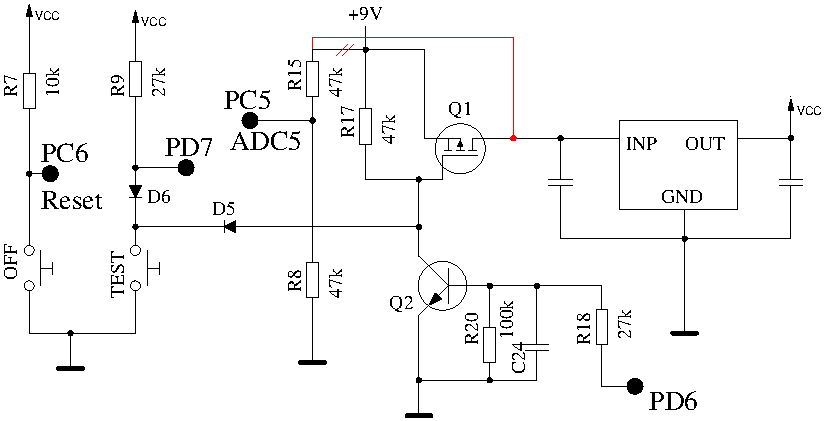
\includegraphics[width=.7\textwidth]{../FIG/Fish8840.pdf}
\caption{Часть схемы версии от Fish8840}
\label{fig:Fish8840}
\end{figure}
Как Вы можете видеть, вместо исходного коэффициента делителя, соотношение сопротивлений резисторов в цепи измерения 
напряжения батареи, R8 и R15 выбрано 2:1.
Кроме того, резистор R15 соединен непосредственно с батареей, что приводит к потреблению энергии в выключенном состоянии. 
Резистор R15 должен быть подключен к стоку Q1 или на вход регулятора напряжения для предотвращения ненужного 
расхода энергии батареи.
Соответствующие изменения в печатной плате изображены на рисунке \ref{fig:Fish8840patch}.
Резистор R15 отсоединён от дорожки, идущей от R17 к D5 и при помощи эмалированной проволоки подсоединён к стоку Q1.
\begin{figure}[H]
\centering
\includegraphics[width=.7\textwidth]{../PNG/Fish8840patch.jpg}
\caption{Вариант изменения в печатной плате Fish8840}
\label{fig:Fish8840patch}
\end{figure}
Коэффициент делителя для измерения напряжения батареи должен быть задан в \lname{Makefile} (например: BAT\_NUMERATOR=66) 
после внесения изменений в оригинальное программное обеспечение.

Для адаптации рабочего напряжения к напряжению контроллера дисплея, модуль дисплея тестера Fish8840 
оснащен регулятором напряжения \(3,3~V\). 
Уровень логических сигналов от ATmega -- \(5~V\). Для адаптации уровня логических
сигналов ATmega к уровню сигналов контроллера дисплея рекомендуется адаптер, изображенный на рисунке~\ref{fig:Fish8840Adapt}.
Сигнальные линии четырех данных оснащены четырьмя резисторами \(2.7~k\Omega\) подсоединёнными последовательно 
для каждого сигнала на небольшой макетной плате. Для подсоединения платы дисплея к плате тестера Fish8840, в 
этом случае, необходимо использовать более длинные или дополнительные межплатные дистанцирующие стойки.
\begin{figure}[H]
  \begin{subfigure}[b]{.5\textwidth}
    \centering
    \includegraphics[width=1.\textwidth]{../PNG/Fish8840Adapt1.jpg}
    \caption{Вид дисплея с адаптером}
  \end{subfigure}
  ~
  \begin{subfigure}[b]{.5\textwidth}
    \centering
    \includegraphics[width=1.\textwidth]{../PNG/Fish8840Adapt2.jpg}
    \caption{Полностью собранный Тестер}
  \end{subfigure}
  \caption{Адаптер для коррекции подключения дисплея}
  \label{fig:Fish8840Adapt}
\end{figure}
Вместо приведенной выше модификации, Вы можете также использовать специальный режим вывода сигналов 
4~SPI ATmega, задав опцию в \lname{Makefile} LCD\_SPI\_OPEN\_COL.
С помощью этой опции, выходы не достигают уровня VCC, так как во время выхода высокого уровня 
подключаются \inquotes{подтягивающие резисторы} на весь период высокого уровня.
Если опция PULLUP\_DISABLE задана, то необходимо установить дополнительный внешний резистор для
сигнала \inquotes{RESET} (PD0).
Поскольку сигналы данных никогда не достигают уровня VCC, уровень \(3,3~V\) контроллера дисплея не 
будет превышен.
В моей версии тестера Fish8840, все сигналы дисплея подключены напрямую к разъему дисплея.
Таким образом, Вы можете подготовить печатную плату для подключения символьного дисплея, если на ней установлен 
ответный разъем и потенциометр для регулировки уровня контрастности.
Однако контакт 15 для подсветки подключается непосредственно к VCC Тестера.
Если Вы подключаете дисплей по такой схеме, Вы должны проверить, наличие ограничительного резистора
подсветки на плате модуля дисплея.
Конечно, Вы должны скомпилировать программное обеспечение для такого подключения дисплея.
Такая аппаратная доработка проверена для платы Fish8840.\\

Все попытки изменить программное обеспечение Вы делаете на свой страх и риск.
Никаких гарантий не может быть дано по поддержанию новых версий.
К сожалению, исходная китайская микропрограмма не может быть сохранена 
из-за установленных битов защиты ATmega328. Так что нет способа вернуть прибор в исходное состояние.\\

Дополнительная версия с графическим дисплеем WEI\_M8 печатной платы изображена на рисунке~\ref{fig:WeiM8}. 
Эта сборка использует аккумулятор LiIon AA размера в качестве источника питания, который может быть 
заряжен от микро USB разъема. 
Эксплуатировать Тестер можно также без аккумулятора, при питании только от USB.
\begin{figure}[H]
\centering
\includegraphics[width=.7\textwidth]{../PNG/WEI_M8.JPG}
\caption{Китайский клон WEI\_M8}
\label{fig:WeiM8}
\end{figure}
Отрадно, что сигнальные линии дисплея (на плате адаптера) оснащены резисторами, включёнными 
последовательно. Вы можете увидеть резисторы на рисунке~\ref{fig:WeiM8int} слева.
Таким образом, Вы не должны бояться, что \(5~V\) сигналы ATmega могут вызвать чрезмерное 
увеличение предельного логического уровня \(3,3~V\) контроллера дисплея.
\begin{figure}[H]
  \begin{subfigure}[b]{.5\textwidth}
    \centering
    \includegraphics[width=1.\textwidth]{../PNG/WEI_M8_D.JPG}
    \caption{Плата адаптера дисплея}
  \end{subfigure}
  ~
  \begin{subfigure}[b]{.5\textwidth}
    \centering
    \includegraphics[width=1.\textwidth]{../PNG/WEI_M8_L.JPG}
    \caption{Основная плата}
  \end{subfigure}
  \caption{Тестер WEI\_M8 в разобранном виде}
  \label{fig:WeiM8int}
\end{figure}
При обновлении до версии 1.12k обнаружены некоторые проблемы.
Если установить Extended Fuse 0x04 (0xFC), как рекомендуется, некоторые измерения вызывали сброс
процессора из-за короткого провала напряжения \inquotes{Brown Out}.
Я добавил дополнительный керамический конденсатор \(4.7~\mu F\) по входу 
регулятора напряжения и \(10~\mu F\) керамический конденсатор на выходе (VCC) регулятора.
И до, и после обновления я заметил, что в биполярных транзисторах, на этой плате, определяется 
дифференциальный ток коллектора (ICEO или ICEs) около \(1\mu A\).
После замены неизвестного LDO регулятора напряжения на MCP1702-5002 этот эффект исчез. 
Рисунок~\ref{fig:WeiM8mod} показывает измененную печатную плату с конденсаторами и регулятором MCP1702, 
установленными навесным монтажом.
Если Вы не желаете прислушиваться к совету, Вы должны установить Extended Fuse 0x07 (0xFF)
для поддержания бесперебойной работы. С этой настройкой кратковременные провалы не будут обнаружены.
\begin{figure}[H]
\centering
\includegraphics[width=.7\textwidth]{../PNG/WEI_M8_modified.JPG}
\caption{Тестер WEI\_M8 после модификации}
\label{fig:WeiM8mod}
\end{figure}
Дополнительная китайская версия с графическим дисплеем -- тестер \inquotes{LCD-T4} 
на печатной плате с жёлтой маской.
Я снял дисплей для замены программного обеспечения на новую версию.
На правом рисунке~\ref{fig:T4_front} Вы можете увидеть в правом верхнем углу отверстия для установки 
ISP разъёма с правильной разводкой для 6-ти контактного подключения программатора.
Для программирования ATmega я не устанавливал штыревой разъём. Я только вставил штыревой разъем  
в отверстия и придержал разъём шлейфа во время программирования.
При таком способе штыревой разъём может быть легко удален и дисплей установлен на место для 
возвращения первоначального вида прибора.
Китайское программное обеспечение может быть заменено на версию 1.12k без каких-либо заметных проблем.
Установка Extended Fuse 0x04 (0xFC) для проверки сброса из-за короткого провала напряжения \inquotes{Brown Out}
каких либо сюрпризов не принесла.
\begin{figure}[H]
  \begin{subfigure}[b]{.5\textwidth}
    \centering
    \includegraphics[width=1.\textwidth]{../PNG/T4_front.JPG}
    \caption{В собранном виде}
  \end{subfigure}
  ~
  \begin{subfigure}[b]{.5\textwidth}
    \centering
    \includegraphics[width=1.\textwidth]{../PNG/T4_front_noLCD.JPG}
    \caption{Со снятым дисплеем}
  \end{subfigure}
  \caption{Внешний вид T4 тестера}
  \label{fig:T4_front}
\end{figure}
Вы можете увидеть стойки \(5~mm\) и обновленные кабели с зажимами измерения на 
фотографии задней стороны на рисунке~\ref{fig:T4_back}.
Поскольку сигналы данных для графического контроллера дисплея не имеют преобразователя
логических уровней (\(5~V\) -\textgreater \ \(3.3~V\)), рекомендуется установить опцию LCD\_SPI\_OPEN\_COL.
В связи с тем, что плата не может быть легко модернизирована \inquotes{pull-up} резисторы могут быть
использованы путем отключения опции PULLUP\_DISABLE в \lname{Makefile}.
Эта плата является меньше практичной для последних расширений, а также замену дисплея 
трудно реализовать.
\begin{figure}[H]
  \begin{subfigure}[b]{.5\textwidth}
    \centering
    \includegraphics[width=1.\textwidth]{../PNG/T4_back.JPG}
    \caption{Сторона компонентов}
  \end{subfigure}
  ~
  \begin{subfigure}[b]{.5\textwidth}
    \centering
    \includegraphics[width=1.\textwidth]{../PNG/T4_back_clips.JPG}
    \caption{С кабелями измерения}
  \end{subfigure}
  \caption{Обратная сторона T4 тестера}
  \label{fig:T4_back}
\end{figure}
Еще одна версия китайского клона с графическим дисплеем имеет название \inquotes{GM328}.
В этой версии адаптер графического индикатора подключен через 16-пиновый разъем к основной плате.
Порт PD5 ATmega подключен через вывод 6 разъема на CE (Chip Enable) вход 
графического контроллера.
Сигнал СЕ также подключен к \(0~V\) (GND) на плате адаптера.
Результатом такого подключения будет короткое замыкание в случае переключения порта PD5 ATmega на
выход \(5~V\).
В новых версиях программного обеспечения выводится сигнал CE, даже если он не является необходимым.
Для правильной работы \inquotes{GM328} тестера с новыми версиями, Вы должны отсоединить сигнал CE (порт PD5 ATmega)
от вывода 6 в разъеме графического адаптера.
\section{Китайские наборы с графическими дисплеями}
Появились две новые версии набора с графическим дисплеем и поворотным энкодером.
Первый набор использует дисплей с контроллером ST7565 или совместимым (128х64 пикселей).
В дополнение к поворотному энкодеру, предусмотрен вход для измерения частоты.
Для тестовых площадок используется 14-контактный разъем Textool, три контакта под пайку
терминалов для подключения кабелей и тестовые площадки для теста деталей SMD.
На фотографии~\ref{fig:Kit_mono} показан смонтированный прибор.
Один из двух нагрузочных конденсаторов кварца \(22~pF\) заменен триммером.
Триммером можно подстроить частоту генерации кварца для повышения точности в режиме частотомера и генератора.
\begin{figure}[H]
  \begin{subfigure}[b]{.5\textwidth}
    \centering
    \includegraphics[width=1.\textwidth]{../PNG/Kit_ST7565a.jpg}
    \caption{смонтированный вид}
  \end{subfigure}
  \begin{subfigure}[b]{.5\textwidth}
    \centering
    \includegraphics[width=1.\textwidth]{../PNG/Kit_ST7565b.jpg}
    \caption{со снятым дисплеем}
  \end{subfigure}
  \caption{Собранный набор с дисплеем 128х64 пикселей}
  \label{fig:Kit_mono}
\end{figure}
Позже появился набор, который использует цветной дисплей с контроллером ST7735 (160x128 пикселей), 
дополнительно оснащен входом для измерения напряжения и выходом для генератора частот.
Но выход генератора не буферизирован, он просто подключен параллельно к контакту ТР2.
Вольтметр может измерять положительное постоянное  напряжение до \(50~V\).
Преобразователь напряжения DC-DC для измерения стабилитронов не предусмотрен.
На фотографиях~\ref{fig:Kit_color} показан этот собранный набор.
Кроме того, в этой версии один нагрузочный конденсатор кварца \(22~pF\) заменен триммером (зеленого цвета).
\begin{figure}[H]
  \begin{subfigure}[b]{.5\textwidth}
    \centering
    \includegraphics[width=1.\textwidth]{../PNG/Kit_Color_a.jpg}
    \caption{смонтированный вид}
  \end{subfigure}
  ~
  \begin{subfigure}[b]{.5\textwidth}
    \centering
    \includegraphics[width=1.\textwidth]{../PNG/Kit_Color_b.jpg}
    \caption{со снятым дисплеем}
  \end{subfigure}
  \caption{Собранный набор с цветным 160x128 пикселей дисплеем}
  \label{fig:Kit_color}
\end{figure}
Оба набора используют ATmega328P в DIP корпусе с установкой в панельку и
не оснащены разъемом ISP для обновления более новыми версиями программного обеспечения.
Первый комплект использует только выводные компоненты для монтажа печатной платы.
Я получил результат измерения резисторов \(680~\Omega\) и \(470~k\Omega\) с допуском 0.1\%\ в
этом китайском комплекте.
Также в набор добавлен конденсатор \(220~nF\) для калибровки.
Комплект с цветным дисплеем оснащён разъемом для подключения внешнего источника питания постоянного тока
вместо \(9~V\) батареи.
Некоторые SMD компоненты были смонтированы на основной плате, так что собрать тестер 
из этого набора не сложная задача.
Небольшой недостаток версии с цветным дисплеем –- скорость вывода на экран.
Особенно это заметно при  перемещении по пунктам меню.
В любом случае, цветной дисплей имеет большее разрешение, что позволяет отобразить больше информации сразу.

Оба набора используют стабилизатор напряжения \(3.3~V\) для питания контроллера
дисплея на плате индикатора.
Только контактный разъем должен быть припаян на печатной плате дисплея.
В цветной версии набора используется буфер CD4050, для адаптации логических уровней сигнала.
Я не обнаружил каких-либо элементов для адаптации уровней сигнала на плате с дисплеем ST7565.
Вероятно, выбранная версия контроллера допускает уровни сигнала \(5~V\) с ATmega328.
Я не обнаружил защитные диоды на входе сигналов со стороны питания \(3.3~V\) для данного типа контроллера.
\section{И еще один клон из Hiland M644}
Эта реплика основана на принципиальной электрической схеме Ника Л. из Украины,
\\см. Иллюстрацию \ref{fig:t644tester} на странице \pageref{fig:t644tester}.\\
\textbf{ Тестер работает с кнопкой, которая является одновременно кнопкой и кодером.}
Предлагает следующие дополнения:

\begin{itemize} \setlength{\itemsep}{-0.5\baselineskip}
 \item частота измерения
 \item генератор f
 \item 10-битный ШИМ
 \item импульсный энкодер
 \item измерение кварца
\item Определение напряжения и десятков диодов (почти до 50В).
\end{itemize}
\vspace{-0.5\baselineskip}
Плата оснащена 8 МГц кварцем. 16 МГц кварц будет лучше
Модифицировать триммер (более точную частоту) сложно.
\\ Контакты для интерфейса ISP находятся в 6-контактном ряду отверстий под
подключаемый модуль дисплея, который занят следующим образом:\\
\textbf{ слева направо}: 1~-сброс; 2~-SCK; 3~-MISO; 4~-MOSI; 5~-+5V; 6~-GND.\\
Чтобы иметь возможность обновить тестер, вам нужен относительно простой кабель
можете создать себя.
При поставке испытательное основание с нулевым усилием соединяется с платой через соединительные планки.

В тестере, показанном ниже, основание было припаяно непосредственно, и полоса сокета сохранена с этим
Припаяны к существующему ленточному кабелю с разъемом и закреплены термоусадочной трубкой.   
\begin{figure}[H]
 \begin{overpic}[width=.64\textwidth]{../FIG/Kabel_Hiland.pdf}
  \color{black}
  \put(14,99){\makebox(0,0)[cb]{Программист}}
  \put(12,-3){\makebox(0,0)[cb]{сообщение разъем}}  
  \put(49,99){\makebox(0,0)[cb]{вид сверху}}
  \put(40,-3){\makebox(0,0)[cb]{ленточный кабель}}  
  \put(90,99){\makebox(0,0)[cb]{Тестер}}
  \put(90,-3){\makebox(0,0)[cb]{Сосуд}}  
 \end{overpic}
 \caption{6 и 10-контактный кабель для программирования}
 \label{fig:Kabel}
\end{figure}

\begin{figure}[H]
  \begin{subfigure}[b]{.47\textwidth}
    \centering
    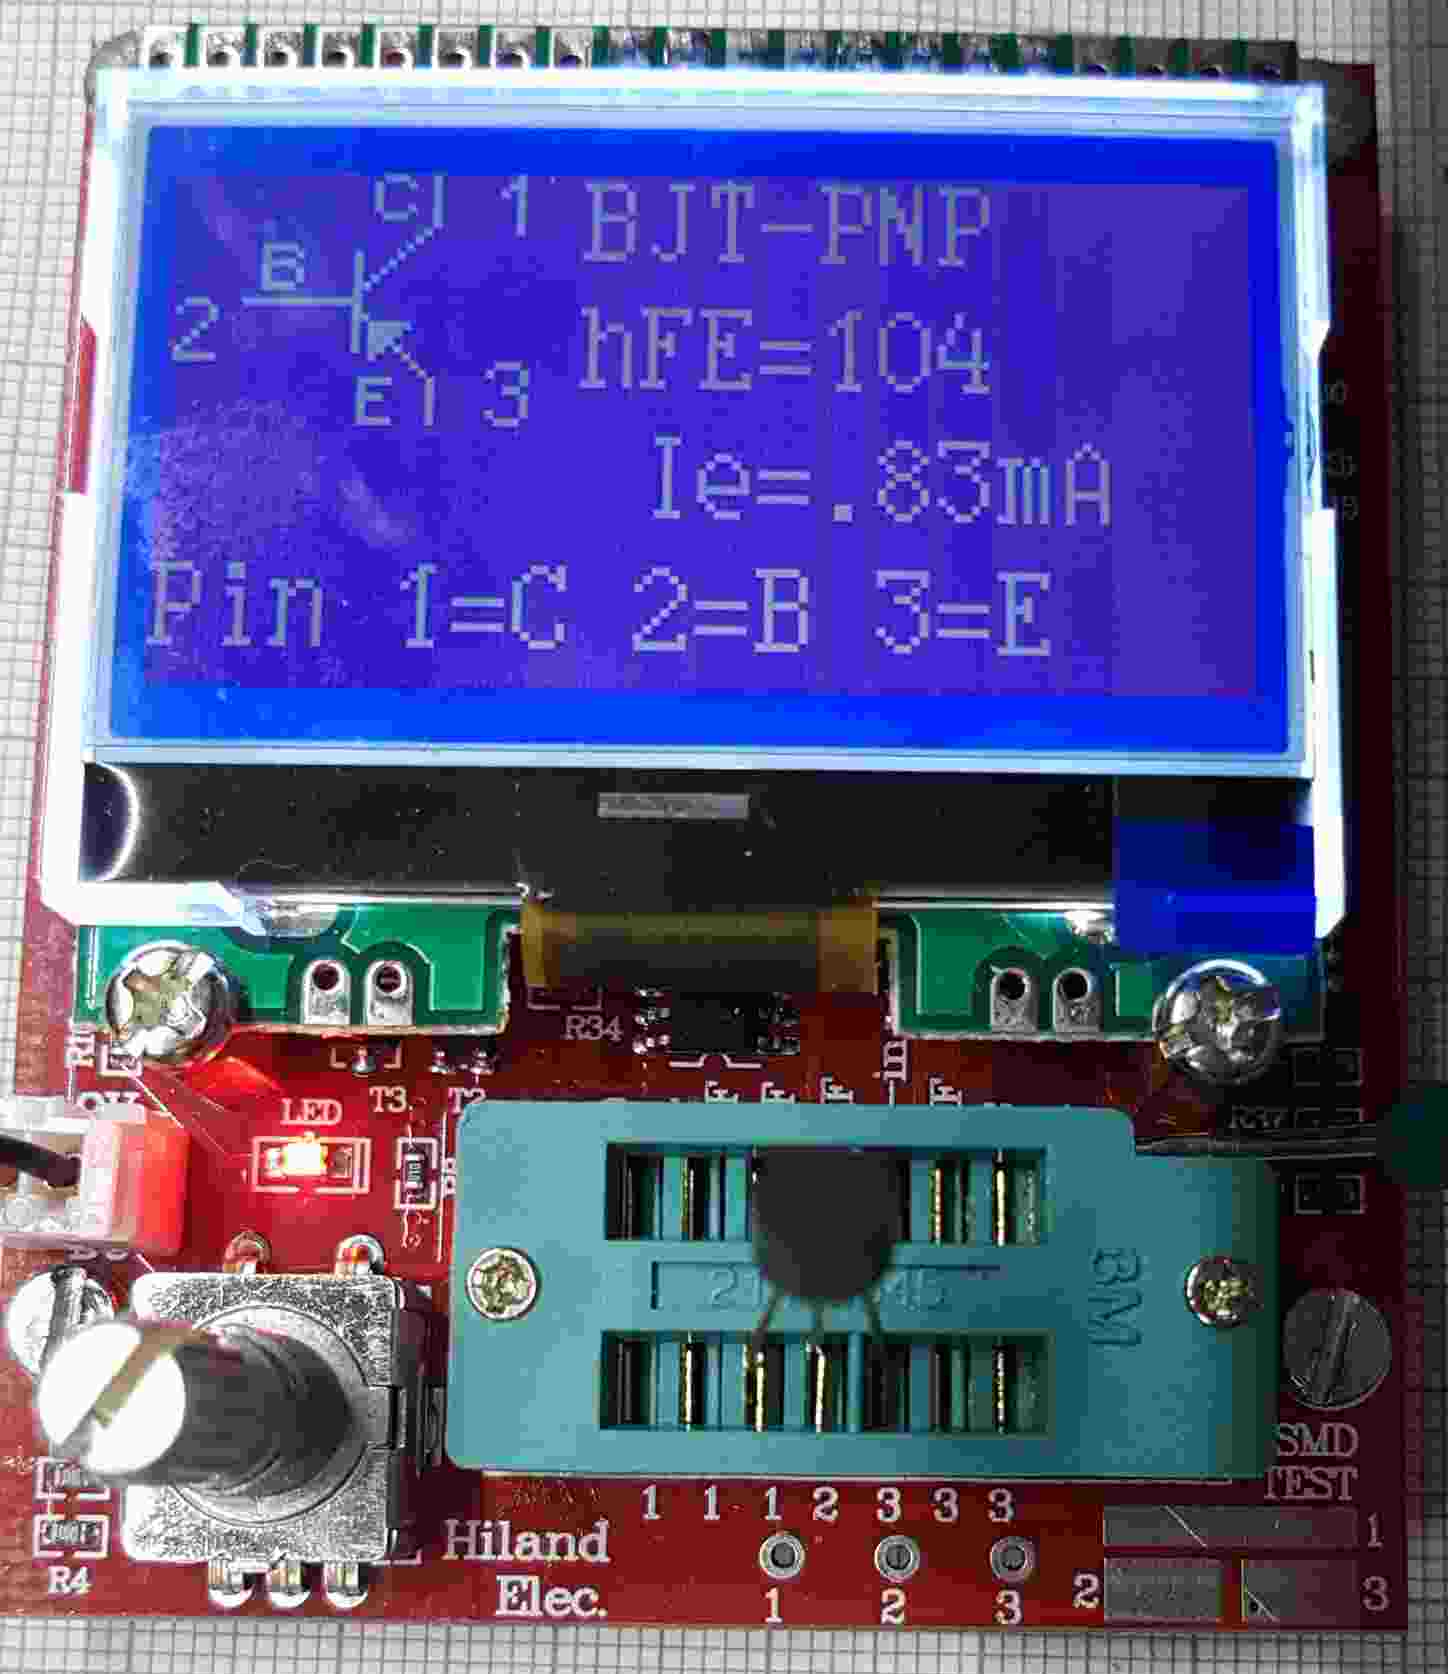
\includegraphics[width=.875\textwidth]{../PNG/Hi_u.jpg}
    \caption{ниже TP1 до TP3 для определения компонента}
  \end{subfigure}
  \begin{subfigure}[b]{.5\textwidth}
    \centering
    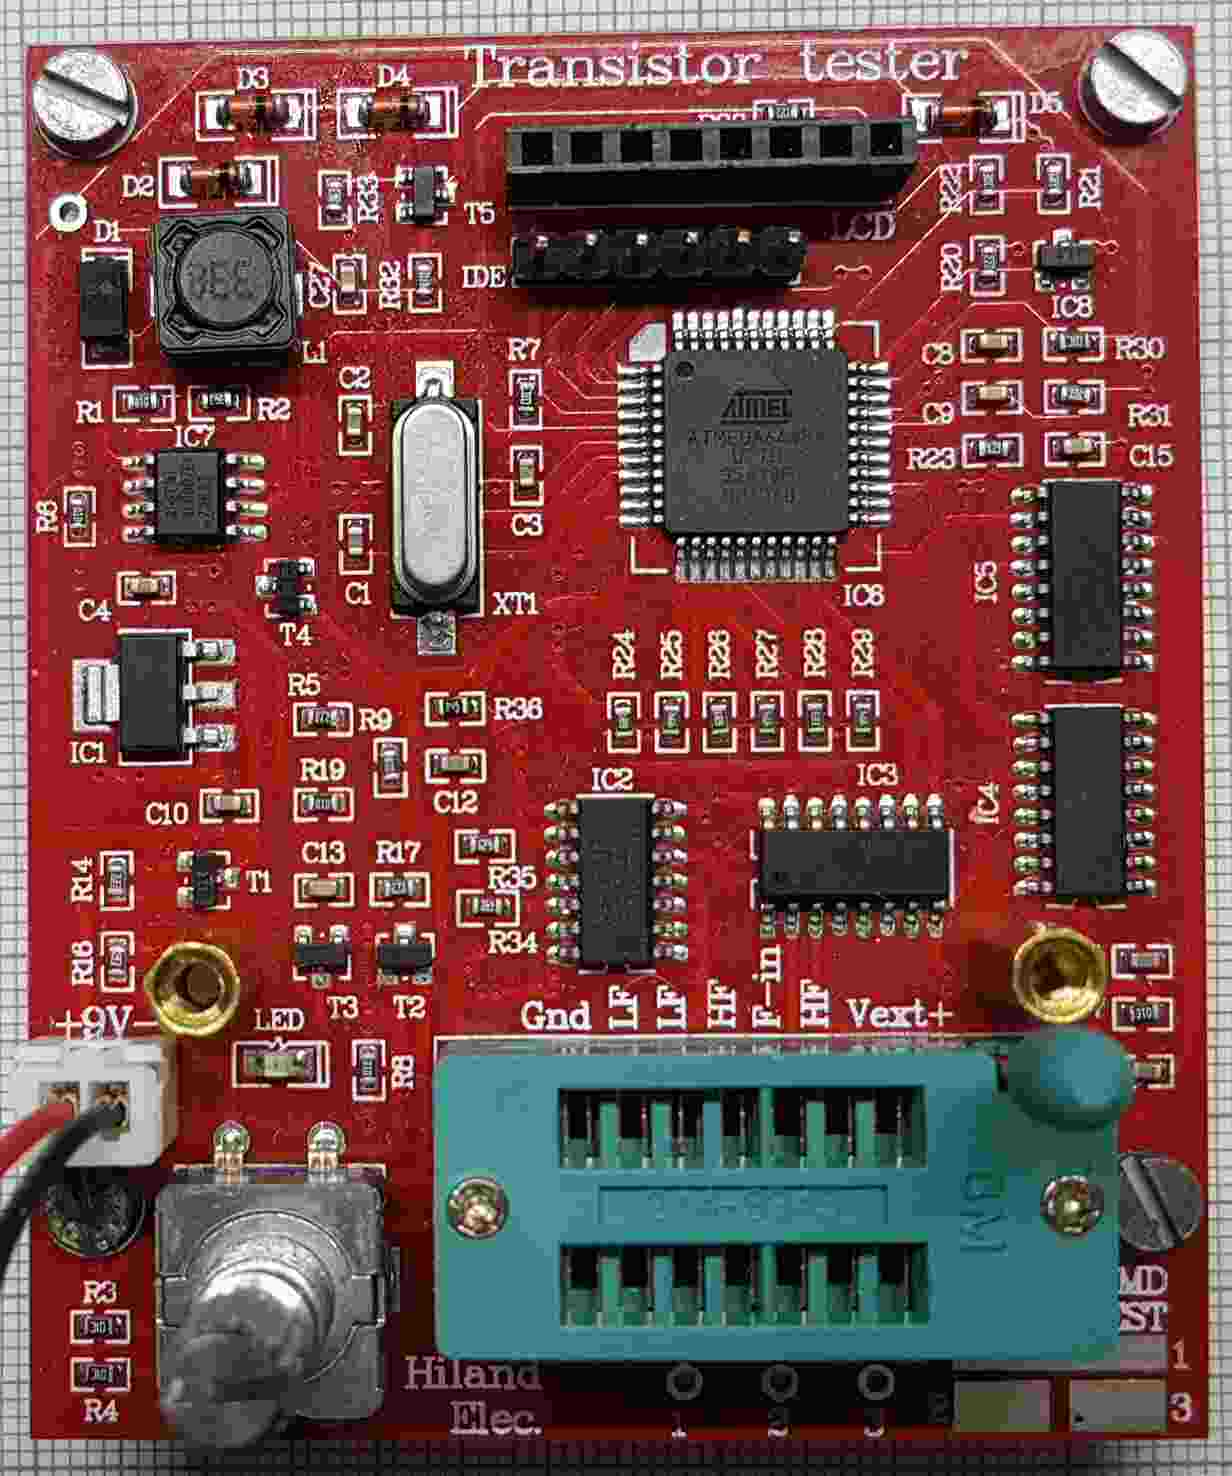
\includegraphics[width=.756\textwidth]{../PNG/Hi_o.jpg}
    \caption{штифты выше для меню выбора и IDE}
  \end{subfigure}
  \caption{Hiland Tester с тестовой базой и дисплеем 128 x 64 пикселей}
  \label{fig:Hiland}
\end{figure}

\textbf{ Тестовые порты TP1, TP2 и TP3}  используются для автоматического распознавания компонентов
и находятся на доске с номерами \textbf{1~~1~~1~~2~~3~~3~~3} в.

То же имя можно найти в поле теста SMD

и есть возможность паять свой собственный тестовый кабель.\\

\textbf{ Testport TP2} также используется для вывода специальной функции "f-Generator". \\
Контакты с маркировкой \textbf{ LF} предназначены для измерения кристаллов кварца с низкой резонансной частотой,
\\ и выводы с меткой \textbf{ HF} предназначены для кристаллов с высокой резонансной частотой.

Пин \textbf{ F-in} используется вместе с \textbf{ Gnd} для частоты специальной функции. \\
И вывод \textbf{ Vext+} также используется с \textbf{ Gnd} для измерения напряжения

\textbf{ и}  использует измерение стабилитрона.


\chapter{Instructions for use}
\label{sec:manual}
\section{The measurement operation}
Using of the Transistor-Tester is simple.
Anyway some hints are required.
In most cases are wires with alligator clips connected to the test ports with plugs.
Also sockets for transistors can be connected.
In either case you can connect parts with three pins to the three test ports in any order.
If your part has only two pins, you can connect this pins to any two of the tree test ports.
Normally the polarity of part is irrelevant, you can also connect pins of electrolytical capacitors in any order. 
The measurement of capacity is normally done in a way, that the minus pole is at the test port with the lower number.
But, because the measurment voltage is only between \(0.3V\) and at most \(1.3V\), the polarity doesn\'t matter.
When the part is connected, you should not touch it during the measurement. You should put it down to a nonconducting pad
if it is not placed in a socket. You should also not touch to the isolation of wires connected with the test ports.
Otherwise the measurement results can be affected.
Then you should press the start button.
After displaying a start message, the measurement result should appear after two seconds.
If capacitors are measured, the time to result can be longer corresponding to the capacity.

How the transistor-tester continues, depends on the configuration of the software.

\begin{description}
  \item[Single measurement mode] If the tester is configured for single measurement mode (POWER\_OFF option), the tester shut off automatical 
after displaying the result for 28~seconds for a longer lifetime of battery. 
During the display time a next measurement can be started by pressing the start button.
After the shut off a next measurement can be started too of course.
The next measurement can be done with the same or another part.
If you have not installed the electronic for automatic shut down, your
last measurement result will be displayed until you start the next measurement.

  \item[Endless measurement mode] A special case is the configuration without automatical shut off.
For this case the POWER\_OFF option is not set in the Makefile.
This configuration is normally only used without the transistors for the shut off function.
A external off switch is necessary for this case. The tester will repeat measurements until power
is switched off.

  \item[Multi measurement mode] In this mode the tester will shut down not after the first measurement but 
after a configurable series of measurements.
For this condition a number (e.g.~5) is assigned to the POWER\_OFF option.
In the standard case the tester will shut down after five
measurements without found part. If any part is identified by test, the tester is shut down after double of
five (ten) measurements. A single measurement with unknown part after a series of measurement of known parts will
reset the counter of known measuerements to zero. Also a single measurement of known part will reset the counter
of unknown measurements to zero. This behavior can result in a nearly endless series of measurements without
pressing the start button, if parts are disconnected and connected in periodical manner.

In this mode there is a special feature for the display period. If the start button is pressed only short for switching
on the tester, the result of measurement ist only shown for 5 seconds. Buf if you press and hold the start button until
the first message is shown, the further measurement results are shown for 28~seconds.
The next measurement can started earlier by pressing the start button during the displaying of result.

\end{description}

\section{Optional menu functions for the ATmega328}
If the menu function is selected, the tester start a selection menu after a long key press (\textgreater~500ms)
for additional functions.
This function is also available for other processors with at least 32K flash memory.
The selectable functions are shown in row two of a 2-line display or as marked function in row 3 of a 4-line display.
The previous and next function is also shown in row 2 and 4 of the display in this case.
After a longer wait time without any interaction the program leave the menu and returns to the normal transistor tester function.
With a short key press the next selection can be shown.
A longer key press starts the shown or marked function.
After showing the last function \inquotes{switch off}, the first function will be shown next.

If your tester has also the rotary pulse encoder installed, you can call the menu with the additional functions
also with a fast rotation of the encoder during the result of a previous test is shown.
The menu functions can be selected with slow rotation of the encoder in every direction.
Starting of the selected menu function can only be done with a key press.
Within a selected function parameters can be selected with slow rotation of the encoder.
A fast rotarion of the encoder will return to the selection menu.

\begin{description} \setlength{\itemsep}{0em}
 \item[frequency]
 The additional function \inquotes{frequency} (frequency measurement) uses the ATmega Pin PD4, which is also connected to the LCD.
First the frequency is allways measured by counting.
If the measured frequency is below \(25kHz\), additionally the mean period of the input signal
is measured and with this value the frequency is computed with a resolution of up to \(0.001Hz\).
By selecting the POWER\_OFF option in the Makefile, the period of frequency measurement is limited to 8~minutes.
The frequency measurement will be finished with a key press and the selectable functions are shown again.\\

 \item[f-Generator]
 With the additional function \inquotes{f-Generator} (frequency generator) you can select output frequencies between 1Hz and 2MHz.
You can change the selected frequency only at the highest shown digit location. 
For the locations 1Hz up to 10kHz digits between 0 and 9 can be selected.
For the highest 100kHz location you can select numericals between 0 and 20.
In row 1 of the frequency line is indicated with the symbol \textgreater~~or \textless~, 
if a longer key press (\textgreater~0.8s) select a higher or lower digit location.
You can only select a lower location (\textless), if the current location has selected the 0 digit and 
if the current location is not the lowest with 1Hz steps.
If you have selected the 100kHz location, the \textgreater~symbol is replaced by a R character. 
A longer key press (\textgreater~0.8s) will result a reset of the frequency value to the initial value of 1Hz in this case.
If the POWER\_OFF option is selected in the Makefile, the key must be pressed longer, because a
short key press (\textless~0.2s) only reset the time limit of 4~minutes.
The elapsed time is shown with a point for every 30 seconds in row 1 of the display.
With periodical short key press you can prevent the time out of the frequency generation.
With a long key press (\textgreater~2s) you will stop the frequency generator and return to the function menu.\\

\item[10-bit PWM]
The additional function \inquotes{10-bit PWM} (Pulse Width Modulation) generates a fixed frequency with selectable
puls width at the pin TP2.
With a short key press (\textless~0.5s) the pulse width is increased by \(1\%\), with a longer key press the pulse width
is increased by \(10\%\).
If \(99\%\) is overstepped, \(100\%\) is subtracted from the result.
If the POWER\_OFF option is selected in the Makefile, the frequency generation is finished after 8~minutes without any key press.
The frequency generation can also be finished with a very long key press (\textgreater~1.3s).\\

\item[C+ESR@TP1:3]
The additional function \inquotes{C+ESR@TP1:3} selects a stand-alone capacity measurement with 
ESR (Equivalent Series Resistance) measurement at the test pins TP1 and TP3. 
Capacities from \(2\mu F\) up to \(50mF\) can be measured. 
Because the measurement voltage is only about \(300mV\), in most cases the capacitor can be
measured \inquotes{in circuit} without previous disassembling.
If the POWER\_OFF option is selected in the Makefile, the count of measurements is limited
to 250, but can be started immediately again.
The series of measurements can be finished with a long key press.\\

 \item[Resistor meter]
With the \mbox{1 \electricR 3} symbol the tester changes to a resistor meter at TP1 and TP3 . 
This operation mode will be marked with a \textbf{[R]} at the right side of the first display line.
Because the ESR measurement is not used in this operation mode, the resolution of the measurement
result for resistors below \(10\Omega\) is only \(0.1\Omega\).
If the resistor measurement function is configured with the additional inductance measurement,
a \mbox{1 \electricR \electricL 3} symbol is shown at this menu.
Then the resistor meter function includes the measurement of inductance for resistors below \(2100\Omega\).
At the right side of the first display line a \textbf{[RL]} is shown.
For resistors below \(10\Omega\) the ESR measurement is used,
if no inductance is find out. For this reason the resolution for resistors below \(10\Omega\) 
is increased to \(0.01\Omega\).
With this operation mode the measurement is repeated without any key press.
With a key press the tester finish this operation mode and returns to the menu.
The same resistor meter function is started automatically, if a single resistor is connected between TP1 and TP3
and the start key was pressed in the normal tester function. In this case the tester returns
from the special mode opration to the normal tester function with a key press.

 \item[Capacitor meter]
With the \mbox{\begin{large}1 \electricC 3\end{large}} symbol the tester changes to a capacitor meter function at TP1 and TP3.
This operation mode will be marked with a \textbf{[C]} at the right side of the first display line.
With this operation mode capacitors from \(1pF\) up to \(100mF\) can be measured.
In this operation mode the measurement is repeated without key press.
With a key press the tester finish this operation mode and returns to the menu.
In the same way as with resistors, the tester changes automatically to the capacitor meter function,
if a capacitor between TP1 and TP3 is measured with the normal tester function.
After a automatically start of the capacitor meter function the tester returns with a key press to
the normal tester function.

\item[rotary encoder]
With the function \inquotes{rotary encoder} a rotary encoder can be checked.
The three pins of the rotary encoder must be connected in any order to the three probes of the transistor tester 
before the start of the function. 
After starting the function the rotary knob must be turned not too fast.
If the test is finished successfully, the connection of the encoder switches  is shown symbolic in display row 2.
The tester finds out the common contact of the two switches and shows, if the indexed position has
both contacts in open state ('o') or in closed state ('C').
A rotary encoder with open switches at the indexed positions is shows in row 2 for two seconds as \inquotes{1-/-2-/-3 o}.
This type of encoder has the same count of indexed positions as count of pulses for every turn. 
Of course the pin number of the right common contact is shown in the middle instead of '2'.
If also the closed switches state is detected at the indexed positions, the row 2 of the display is also
shown as \inquotes{1---2---3 C} for two seconds.
I don't know any rotary encoder, which have the switches always closed at any indexed position.
The interim state of the switches between the indexed positions is also shown in row 2 for a short time (\textless\(~0.5s\))
without the characters 'o' or 'C'.
If you will use the rotary encoder for handling the tester, you should set the Makefile option WITH\_ROTARY\_SWITCH=2
for encoders with only the open state ('o') and set the option WITH\_ROTARY\_SWITCH=1 for encoders 
with the open ('o') and closed ('C') state at the indexed positions.\\

\item[C(\(\mu F\))-correction]
With this menu function you can change a correction factor for bigger capacity values.
You can preset the same factor with the Makefile option C\_H\_KORR.
Values above zero reduce the output value of the capacity with this percent value, values below zero will increase
the shown capacity value. A short key press will reduce the correction value about 0.1\%, a longer key press will
increase the correction value. A very long key press will save the correction value.
It is a characteristic of the used measurement method, that capacitors with low quality like electrolytic type will
result to a too high capacity value. You can detect a capacitor with low quality by a higher value of the Vloss parameter.
High quality capacitors have no Vloss or only 0.1\%.
For adjusting this parameter you should only use capacitors with high quality and a capacity value above \(50\mu F\).
By the way the exactly capacity value of electrolytic capacitors is unimportant, because the capacity value differ
with temperature and DC-voltage.

\item[Selftest]
With the menu function \inquotes{Selftest} a full selftest with calibration is done.
With that call all the test functions T1 to T7 (if not inhibited with the NO\_TEST\_T1\_T7 option) 
and also the calibration with external capacitor is done every time.\\

\item[Voltage]
The additional function \inquotes{Voltage} (Voltage measurement) is only possible, if the serial output is deselected
or the ATmega has at least 32 pins (PLCC) and one of the additional pins ADC6 or ADC7 is used for the measurement.
Because a 10:1 voltage divides is connected to PC3 (or ADC6/7), the maximum external voltage can be \(50V\).
A installed DC-DC converter for zener diode measurement can be switched on by pressing the key.
Thus connected zener diodes can be measured also.
By selecting the POWER\_OFF option in the Makefile and without key pressing, the period of voltage measurement is limited to 4~minutes.
The measurement can also be finished with a extra long key press (\textgreater~4~seconds).

\item[Contrast] 
This function is available for display controllers, which can adjust the contrast level with software.
The value can be decreased by a very short key press or left turn with the rotary encoder.
A longer key press (\textgreater~0.4s) or a right turn of the rotary encoder will increase the value.
The function will be finished and the selected value will be saved nonvolatile in the EEprom memory 
by a very long key press (\textgreater~1.3s).

\item[BackColor]
For color displays this menu item can be enabled with the Makefile option LCD\_CHANGE\_COLOR 
for selecting the background color. The rotary encoder extension must be installed.
You can select the colors red, green and blue with a longer key press. The intensity value of the
selected color, which is marked with a {\textgreater} symbol in column 1, can be changed by a turn of the rotary encoder.

\item[FrontColor]
For color displays this menu item can be enabled with the Makefile option LCD\_CHANGE\_COLOR 
for selecting the foreground color. The rotary encoder extension must be installed.
You can select the colors red, green and blue with a longer key press. The intensity value of the
selected color, which is marked with a {\textgreater} symbol in column 1, can be changed by a turn of the rotary encoder.

 \item[Show data]
 The function \inquotes{Show Data} shows besides the version number of the software the data of the calibration.
These are the zero resistance (R0) of the pin combination 1:3, 2:3 and 1:2 .
In addition the resistance of the port outputs to the \(5V\) side (RiHi) and
to the \(0V\) side (RiLo) are shown.
The zero capacity values (C0) are also shown with all pin combinations (1:3, 2:3, 1:2 and 3:1, 3:2 2:1).
Next the correction values for the comparator (REF\_C) and for the reference voltage (REF\_R) are also shown.
With graphical displays the used icons for parts and the font set is also shown.
Every page is shown for 15 seconds, but you can select the next page by a key press or a right turn of the rotary encoder.
With a left turn of the rotary encoder you can repeat the output of the last page or return to the previous page.


\item[Switch off]
With the additional function \inquotes{Switch off} the tester can be switched off immediately.\\

\item[Transistor]
Of course you can also select the function \inquotes{Transistor} (Transistor tester) to return to a normal Transistor tester measurement. 
\end{description}

With the selected POWER\_OFF option in the Makefile, all additional functions are limited in time without interaction to prevent a discharged battery.


\section{Selftest and Calibration}

If the software is configured with the selftest function, the selftest can be prepared by connecting all three
test ports together and pushing of the start button.
To begin the self test, the start butten must be pressed again within 2 seconds, or else the tester will continue
with a normal measurement.

If the self test is started, all of the documented tests in the Selftest chapter~\ref{sec:selftest} will be done.
If the tester is configured with the menu function (option WITH\_MENU), 
the full selftest with the tests T1 to T7 are only done with the \inquotes{Selftest} function, 
which is selectable as menu function.
In addition the calibration with the external capacitor is done with every call from function menu,
otherwise this part of calibration is only done first time.
Thus the calibration with the automatically started selftest (shorted probes) can be done faster.
The repetition of the tests T1 to T7 can be avoided, if the start button is hold pressed.
So you can skip uninteresting tests fast and you can watch interresting tests by releasing the start button.
The test 4 will finish only automatically if you separate the test ports (release connection).

If the function AUTO\_CAL is selected in the Makefile, 
the zero offset for the capacity measurement will be calibrated with the selftest.
It is important for the calibration task, that the connection between the three test ports is relased 
during test number 4. 
You should not touch to any of the test ports or connected cables when calibration (after test 6) is done.
But the equipment should be the same, which is used for further measurements.
Otherwise the zero offset for capacity measurement is not detected correctly.
The resistance values of port outputs are determined at the beginning of every measurement with this option.\\

If you have selected the samplingADC function in the Makefile with the option \inquotes{WITH\_SamplingADC = 1},
two special steps are included to the calibration precedure.
After the normal measuring of the zero capacity values, also the zero capacity values for the samplingADC function is
measured (C0samp). As last step of the calibration the connection of a test capacitor at pin~1 and pin~3 is requested for
later measurement of little coils with the message \mbox{\begin{large}1 \electricC 3~10-30nF[L]\end{large}}.
The capacity value should be between \(10nF\) and \(30nF\),
to get a measurable resonant frequency by later parallel connection to a coil with less than \(2mH\).
For inspection of coils with more than \(2mH\) inductance the normal measurement method should result to a
sufficient accuracy. The parallel connection of the capacitor to use the other measurement method should
not be usefull.\\

A capacitor with any capacity between \(100nF\) and \(20\mu F\) connected to pin~1 and pin~3 is
required after the measurement of the zero capacity values.
To indicate that, the message \mbox{\begin{large}1 \electricC 3~\textgreater 100nF\end{large}} is shown in row 1 of the display.
You should connect the capacitor not before the message C0= or this text is shown.
With this capacitor the offset voltage of the analog comparator will be compensated for better measurement
of capacity values.  
Additionally the gain for ADC measurements using the internal reference voltage will be adjusted too 
with the same capacitor for better resistor measurement results with the AUTOSCALE\_ADC option.
If the menu option is selected for the tester and the selftest is not started as menu function,
the calibration with the external capacitor is only done for the first time calibration.
The calibration  with the external capacitor can be repeated with a selftest call as menu selection.

The zero offset for the ESR measurement will be preset with the option ESR\_ZERO in the Makefile.
With every self test the ESR zero values for all three pin combinations are determined.
The solution for the ESR measurement is also used to get the values of resistors below \(10\Omega\) with
a resolution of \(0.01\Omega\).


\section{special using hints}
Normally the Tester shows the battery voltage with every start. If the voltage fall below a limit,
a warning is shown behind the battery voltage. If you use a rechargeable \(9V\) battery, you should replace
the battery as soon as possible or you should recharge.
If you use a tester with attached \(2.5V\) precision reference, the measured supply voltage will be shown
in display row two for 1 second with \inquotes{VCC=x.xxV}.

It can not repeat often enough, that capacitors should be discharged before measuring.
Otherwise the Tester can be damaged before the start button is pressed.
If you try to measure components in assembled condition, the equipment should be allways disconnected from power source.
Furthermore you should be sure, that no residual voltage reside in the equipment.
Every electronical equipment has capacitors inside!

If you try to measure little resistor values, you should keep the resistance of plug connectors and cables in mind.
The quality and condition of plug connectors are important, also the resistance of cables used for measurement.
The same is in force for the ESR measurement of capacitors.
With poor connection cable a ESR value of \(0.02\Omega\) can grow to \(0.61\Omega\).
If possible, you should connect the cables with the test clips steady to the tester (soldered).
Then you must not recalibrate the tester for measuring of capacitors with low capacity values,
if you measure with or without the plugged test cables. 
For the calibration of the zero resistance there is normaly a difference, if you connect the
three pins together directly at a socket or if you connect together the test clips at the end of cables.
Only in the last case the resistance of cables and clips is included in the calibration.
If you are in doubt, you should calibrate your tester with jumpers directly at the socket 
and then measure the resistance of shorten clips with the tester.

You should not expect very good accuracy of measurement results, especially the ESR measurement and the results of inductance measurement are not very exact.
You can find the results of my test series in chapter~\ref{sec:measurement} at page~\pageref{sec:measurement}.

\section{Compoments with problems}
You should keep in mind by interpreting the measurement results, that the circuit of the TransistorTester is
designed for small signal semiconductors. In normal measurement condition the measurement current can only reach about \(6mA\).
Power semiconductors often make trouble by reason of residual current with the identification an the measurement of junction capacity value.
The Tester often can not deliver enough ignition current or holding current for power Thyristors or Triacs.
So a Thyristor can be detected as NPN transistor or diode. Also it is possible, that a Thyristor or Triac is detected as unknown.

Another problem is the identification of semiconductors with integrated resistors.
So the base - emitter diode of a BU508D transistor can not be detected by reason of the parallel connected
internal \(42\Omega\) resistor.
Therefore the transistor function can not be tested also.
Problem with detection is also given with power Darlington transistors. We can find often internal
base - emitter resistors, which make it difficult to identify the component with the undersized measurement current.

\section{Measurement of PNP and NPN transistors}
For normal measurement the three pins of the transistor will be connectet in any order to the measurement
inputs of the TransistorTester.
After pushing the start button, the Tester shows in row 1 the type (NPN or PNP), 
a possible integrated protecting diode of the Collector - Emitter path and the
sequence of pins. The diode symbol is shown with correct polarity.
Row 2 shows the current amplification factor \(B\) or \(hFE\) and the current, by which the
amplification factor is measured. If the common emitter circuit is used for the hFE determinatation,
the collector current \(Ic\) is output. If the common collector circuit is used for measuring of the
amplification factor, the emitter current \(Ie\) is shown.
Further parameters are shown for displays with two lines in sequence, one after the the other in line 2.
For displays with more lines further parameters are shown directly until the last line is allready used.
When the last line is allready used before, the next parameter is shown also in the last line
after a time delay automatically or earlier after a key press.
If more parameters are present than allready shown, a + character is shown at the end of the last line.
The next shown parameter is anyway the Base - Emitter threshold voltage.
If any collector cutoff current is measurable, the collector current without base current \(I_CE0\)
and the collector current with base connected to the emitter \(I_CES\) is also shown.
If a protecting diode is mounted, the flux voltage \(Uf\) is also shown as last parameter.


With the common Emitter circuit the tester has only two alternative to select the base current:
\begin{enumerate}
\item The \(680\Omega\) resistor results to a base current of about \(6.1mA\). 
This is too high for low level transistors with high amplification factor, because the base is saturated.
Because the collector current is also measured with a \(680\Omega\) resistor, the collector current
can not reach the with the amplification factor higher value.
The software version of Markus F. has measured the Base - Emitter threshold voltage in this ciruit (Uf=...).\\
\item The \(470k\Omega\) resistor results to a base current of only \(9.2\mu A\) .
This is very low for a power transistor with low current amplification factor.
The software version of Markus F. has identified the current amplification factor with this circuit (hFE=...).\\
\end{enumerate}

The software of the Tester figure out the current amplification factor additionally with the common Collector circuit.
The higher value of both measurement methodes is reported.
The common collector circuit has the advantage, that the base current is reduced by negative current feedback corresponding
to the amplification factor. 
In most cases a better measurement current can be reached with this methode for power transistors
with the \(680\Omega\) resistor and for Darlington Transistors with \(470k\Omega\) resistor.
The reported Base - Emitter threshold voltage Uf is now measured with the same current used 
for determination of the current amplification factor.
However, if you want to know the Base - Emitter threshold voltage with a measurement current of about \(6mA\),
you have to disconnect the Collector and to start a new measurement.
With this connection, the Base - Emitter threshold voltage at \(6mA\) is reported. The capacity value
in reverse direction of the diode is also reported.
Of course you can also analyse the base - collector diode.

With Germanium transistors often a Collector cutoff current \(I_{CE0}\) with currentless base or 
a Collector residual current \(I_{CES}\) with base hold to the emitter level is measured.
Only for ATmega328 processors the Collector cutoff current is shown in this case at the row 2 of the LCD 
for 5 seconds or until the next keypress before showing the current amplification factor. 
With cooling the cutoff current can be reduced significant for Germanium transistors.


\section{Measurement of JFET and D-MOS transistors}
Because the structure of JFET type is symmetrical, the Source and Drain of this transistores can not
be differed.
Normally one of the parameter of this transistor is the current of the transistor with the Gate at the same level as Source.
This current is often higher than the current, which can be reached with the measurement circuit of the TransistorTester
with the \(680\Omega\) resistor.
For this reason the \(680\Omega\) resistor is connected to the Source. Thus the Gate get with the growing of current a negative
bias voltage.
The Tester reports the Source current of this circuit and additionally the bias voltage of the Gate.
So various models can be differed.
The D-MOS transistors (depletion type) are measured with the same methode.

\section{Measurement of E-MOS transistors and IGBTs}
You should know for enhancement MOS transistors (P-E-MOS or N-E-MOS), that the measurement of the gate threshold voltage (Vth)
is more difficult with little gate capacity values. You can get a better voltage value, if you connect a capacitor with a value
of some nF parallel to the gate /source.
The gate threshold voltage will be find out with a drain current of about \(3.5mA\) for a P-E-MOS and about \(4mA\) for a N-E-MOS.
The RDS or better R\textsubscript{DSon} of E-MOS transistors is measured with a gate - source voltage of nearly \(5V\),
which is probably not the lowest value.
In addition, the RDS resistance is determined at a low drain current, which limits the resolution of the resistance value.
Often in the case of IGBTs and sometimes also withn enhancement MOS transistors, the available \(5V\) of the tester
is not sufficient to drive the transistor across the gate.
In this case, a battery with about \(3V\) will help to make a detection and measurements with the tester possible.
The battery is connected to the gate of the transistor with one pole and the other pole of the battery
is then connected to a test port (TP) of the tester instead of the transistor gate.
When the battery is correctly polarized, the battery voltage is added to the control voltage of the tester and
the detection of the transistor succeeds.
The battery voltage must then be added to the indicated gate threshold voltage of course,
in order to get the correct threshold voltage for this component


\section{Measurement of capacitors}
The capacity values are always computed from the time constant, which is build by the serial connection of the
build in resistors with the capacitor during charging. With little capacity values the \(470k\Omega\) resistors are
used for the measurement the time to reach a threshold voltage.
For bigger capacity values with some \(10\mu F\) the voltage grow at the capacitor is monitored after charge pulses with the
\(680\Omega\) resistors. With this voltage grow the capacity can be computed together with the count of fixed length pulses.
Very low capacity values can be measured with the samplingADC method.
For analysing the same load pulse is repeated many times and the voltage is monitored with the time shift of the ADC S\&H time
using interval-tics build from the processor clock. But a complete AD conversion take 1664 processor tics!
Up to 250 ADC samples are build by this way and from the voltage curve the capacity value is computed.
If the samplingADC function is selected in the Makefile, all capacitors with less than \(100pF\) are measured with
the samplingADC function in the capacitor-meter mode \textbf{[C]}. The resolution is up to \(0.01pf\) with a clock 
frequency of \(16MHz\). The calibrated condition is difficult to build with this high resolution.
You can assume the use of the samplingADC methode every time, fractions of \(1pF\) are displayed at the screen.
By the way it should mentiored, that the junction capacitance of single diodes can also be measured with
this method. Because this method can measure the capacity value by charging or discharging, two capacity results are shown.
Both values differ be reason of the capacity diode effect.

\section{Measurement of coils}
The normal measurement of the inductance is based on the measurement of the time constant of the current grow.
The detection limit is about \(0.01mH\), if the resistance of the coil is below \(24\Omega\).
For bigger resistance values the resolution is only \(0.1mH\).
If the resistance is above \(2.1k\Omega\), this technique can never be used to detect coils.
The measurement results of this normal measurement is shown in the second line (resistance and inductance).
With the samplingADC method a resonant frequency of coils can be detected with greater inductance values.
If this effect is noticeable, the frequency and the quality factor Q of the coil is shown additionally in line 3. 

The method of resonant frequency measurement can also be used for the determination of the inductance value,
if a sufficient big capacitor mith know capacity value is connected parallel to a little inductance (\textless\(2mH\)).
With a parallel connected capacitor the normal measurement of inductance can no more operate well.
If the resonant frequency let assume a parallel connected capacitor, the inductance of the normal measurement
is not shown and the resistance value is shown in line 1.
For this resonant circuit the quality factor Q is also computed and shown behind the frequency value in line 3.
You can identify this type of measurement with the inductance value at the first position of line 2,
followed by the text \inquotes{ if } and the value of the assumed parallel capacity.
The value of this parallel capacitor can currently only be set with the calibration function (\mbox{\begin{large}1 \electricC 3~10-30nF(L)\end{large}}).

For displays with only two lines, the content for the third line is shown time-delayed in line 2.


\chapter{Programming of the TransistorTester}
\section{Configuring the TransistorTester}
\label{sec:config}
The complete software for the TransistorTester is available in source code.
The compilation of modules is controlled with a Makefile. The developement was done
at the Ubuntu Linux operating system with the GNU toolchain (gcc version 4.5.3).
It should be possible to use other Linux operating systems without problems.
To load the compiled data to the flash memory or
the EEprom memory, the tool avrdude (version 5.11svn) was taken by the Makefile, if you call ''make upload''.
 The program avrdude \cite{avrdude} is available for Linux and Windows operating system.
The gnu C-compiler gcc is also taken by the AVR studio software and
by the WinAVR \cite{winavr1},\cite{winavr2} software at the Windows operating system.
You can load the program data (.hex and .eep) also with other tools to the ATmega,
but only my Makefile version takes care to load the correct data to the choosed processor.
Avrdude loads only data to the ATmega if the Signature Bytes of the connected ATmega is
identical to the choosed one. 
If you alter the Makefile, all the software will be compiled new, if you call a ''make'' or
''make upload'' command. The software compiled for a ATmega8 does not run on a ATmega168.
The software compiled for a ATmega328 does not run on the ATmega168! 
A exeption from this rule is the software compiled for ATmega168, this data can also be used
for a ATmega328 without changes.
Be careful, if you don't use my Makefile.

With the correct options set, my software runs on the unchanged hardware of Markus F.
You must set the option PARTNO=M8, {\bf NOT} the option NO\_AREF\_CAP and {\bf NOT} the  PULLUP\_DISABLE option.
The clock rate can also be set to \(8MHz\) with fuses, no crystal is required!


The following options in the Makefile are avaiable to configure the software for your Tester.

\begin{description}
  \item[PARTNO] describes the target processor:\\
         m8 = ATmega8\\
         m168 or m168p = ATmega168\\
         m328 or m328p = ATmega328\\
         m644 or m644p = ATmega644\\
         m1284p        = ATmega1284\\
         m1280         = ATmega1280\\
         m2560         = ATmega2560\\
    Example:  PARTNO = m168
   \item[UI\_LANGUAGE] specifies the favored Language\\
    LANG\_BRASIL, LANG\_CZECH, LANG\_DANISH, LANG\_DUTCH, LANG\_ENGLISH, \\
    LANG\_GERMAN, LANG\_HUNGARIAN, LANG\_ITALIAN, LANG\_LITHUANIAN, \\
    LANG\_POLISH, LANG\_RUSSIAN, LANG\_SLOVAK, LANG\_SLOVENE, \\
    LANG\_SPANISH  and LANG\_UKRAINIAN is currently avaiable.
 The russian or ukrainian language requires a LCD with cyrillic character set.\\
    Example:  UI\_LANGUAGE = LANG\_ENGLISH

  \item[LCD\_CYRILLIC] is only needed for a LCD-display with cyrillic character set. The \(\mu\) and \(\Omega\) character
is not avaiable with the cyrillic character set.
If you specify this option, both characters are loaded to the LCD with software.
You should set this option, if your display shows wrong characters instead of \(\mu\) or \(\Omega\).\\
Example: CFLAGS += -DLCD\_CYRILLIC

 \item[LCD\_DOGM] must be set, if a LCD with ST7036 controller (Type DOG-M) is used for displaying.
The LCD-contrast is then set with software commands.
If you have changed the contrast value to a wrong value, so that you can not read anything at your display,
you shouls first try to read somthing from a side look to the display.
If this fails also, you should reset the EEprom to the initial values with a ISP programmer.\\
Example: CFLAGS += -DLCD\_DOGM

 \item[FOUR\_LINE\_LCD] can be used with a 4x20 character display for better using the additional space.
Additional parameters, which are shown only short in row 2, will be shown in row 3 and 4 with this option.\\
Example: CFLAGS += -DFOUR\_LINE\_LCD

  \item[DD\_RAM\_OFFSET] Somne character displays use different DD-RAN starting addresses for the beginning of each line.
Usually the DD-RAM starting address for line 1 is 0.
Some displays like TC1604 or TC1602 use a 128 (0x80) for the beginning of line 1.
This can be respected with this option.
Example: CFLAGS += -DDD\_RAM\_OFFSET = 128

  \item[WITH\_LCD\_ST7565] This option must be used, if a 128x64 pixel LCD is connected with serial
interface. For this display type further options must be set, which are described in table~\ref{tab:cod-display}.
You can also use the simular SSD1306 controller instead of the ST7565 controller for example.
This must be done by setting the variable WITH\_LCD\_ST7565 to 1306.
A PCF8812 or PCF8814 Controller is also supported, if the Option is set correctly.
Also a display with a ST7920 or NT7108 controller can be connected.
For the NT7108 controller a additional serial-parallel converter 74HC(T)164 or 74HC(T)595 must be used.  \\
Example: WITH\_LCD\_ST7565 = 1 

 \item[LCD\_INTERFACE\_MODE] For the SSD1306 controller also the I\textsuperscript{2}C type interface with address 0x3c
can be used  instead of the 4-wire SPI interface by setting this option to 2.
For the ST7920 controller a special serial interface can be selected by setting this option to 5.
If only one connection type is provided for a controller, you need not set the constant LCD\_INTERFACE\_MODE .
All currently used values for LCD\_INTERFACE\_MODE and WITH\_LCD\_ST7565 are shown in table~\ref{tab:cod-display}. \\

\begin{table}[H]
  \begin{center}
    \begin{tabular}{| c | c | c | c|}
    \hline
 Display-Type       &  Interface       & WITH\_LCD\_ST7565 &  LCD\_INTERFACE\_MODE \\
    \hline
    \hline
  Character 16x2,   & 4-Bit parallel   &  disabled (0)     & disabled (1) \\
  Character 20x4    &  4-Bit SPI       &                   &    4   \\
                  & I\textsuperscript{2}C &                &   2    \\
    \hline
  Graphic ST7565    & 4-Bit SPI        &   1 or 7565       &  disabled (4) \\
    \hline
  Graphic ST7565  & I\textsuperscript{2}C & 1 or 7565      &   2 \\
    \hline
  Graphic SSD1306   & 4-Bit SPI        &   1306            &  disabled (4) \\
    \hline
  Graphic SSD1306  & I\textsuperscript{2}C & 1306          &   2 \\
    \hline
  Graphic ST7920    & 4-Bit parallel   &   7920            &  disabled (1) \\
    \hline
  Graphic ST7920    & 2-Bit serial     &   7920            &  5 \\
    \hline
  Graphic NT7108    & 8-Bit parallel   &   7108            &  disabled (6) \\
    or KS0108       &    + 74HCT164    &                   &      \\
    \hline
  Graphic PCF8812   & SPI              &   8812            & disabled (4) \\
    \hline
  Graphic PCF8814   & SPI              &   8814            & disabled (4) \\
                  & I\textsuperscript{2}C & 8814           &   2 \\
                    & 3-line           &   8814            &   3 \\
    \hline
  Graphic ILI9163   & SPI             & 9163              & disabled (4) \\
  128x128 Color     &                 &                   &              \\
    \hline
  Graphic ST7735    & SPI             & 7735              & disabled (4) \\
  128x160 Color     &                 &                   &              \\
    \hline
    \end{tabular}
  \end{center}
  \caption{Number setting for controller and interface mode}
  \label{tab:cod-display}
\end{table}

The values in brackets are used software internal and are shown for information only.
You should not set the values in brackets here in the Makefile.\\

Example: CFLAGS += -DLCD\_INTERFACE\_MODE=2

  \item[LCD\_SPI\_OPEN\_COL] With the option LCD\_SPI\_OPEN\_COL the data signals of the SPI interface
are not switched to VCC directly.
The signals are switched to GND only, for high signals the pullup resistors of the ATmega are used.
For the RESET signal a external pull-up resistor is required, if the option PULLUP\_DISABLE is set.
For the other signals the internal pullup resistors of the ATmega are temporary used,
even if option PULLUP\_DISABLE is set.
Example: CFLAG += -DLCD\_SPI\_OPEN\_COL

\item[LCD\_I2C\_ADDR] The I\textsuperscript{2}C address of the SSD1306 controller can be selected to 0x3d by presetting
the constant LCD\_I2C\_ADDR to 0x3d.\\
Example: CFLAGS += -DLCD\_I2C\_ADDR=0x3d

  \item[LCD\_ST7565\_RESISTOR\_RATIO] With this option the resistor ratio for the voltage regulator of
the ST7565 controller is set.
Usually values between 4 and 7 are practical.
The value can be set between 0 and 7.\\
Example: LCD\_ST7564\_RESISTOR\_RATIO = 4

  \item[LCD\_ST7565\_H\_FLIP] With this option the display content can be flipped in horizontal direction.\\
Example: CFLAGS += -DLCD\_ST7565\_H\_FLIP = 1

  \item[LCD\_ST7565\_H\_OFFSET] This option can be used to adapt the display window to the used memory area.
 The controller uses more horizontal pixel (132) as the display window shows (128).
 Depending of your display module a value of 0, 2 or 4 can be required for proper presentation.\\
Example: CFLAGS += -DLCD\_ST7565\_H\_OFFSET = 4

  \item[LCD\_ST7565\_V\_FLIP] With this option the display content can be flipped in vertical direction.\\
Example: CFLAGS += -DLCD\_ST7565\_V\_FLIP = 1

  \item[VOLUME\_VALUE] You can predefine a contrast value for ST7565 or SSD1306 controllers.
The value for the ST7565 controller can be between 0 and 63. For the SSD1306 controller you can
select a value between 0 and 255.\\
Example: CFLAGS += -DVOLUME\_VALUE = 25

  \item[LCD\_ST7565\_Y\_START] With this option you can set the first row correctly to the top of screen.
The first row is shifted to the middle of the screen for some display variants.
For this variants you can shift the first row to the top of the screen again,
if this option is set to 32 (half of the screen height).\\
Example: CFLAGS += -DLCD\_ST7565\_Y\_START = 32

  \item[LCD\_CHANGE\_COLOR] This option expand the menu functions with a selection item
to change the background and the foreground color.
If the value is set to 2, the colors blue and red are swapped.
You can select this option only for color displays (controller ST7735 or ILI9163).\\
Example: CFLAGS += -DLCD\_CHANGE\_COLOR=1

 \item[LCD\_BG\_COLOR] With this 16-bit value you can select a background color.
Normally the upper 5 bits are used for the color red, the middle 6 bits are used for the color green
and the lower 5 bits are used for the color blue. Sometimes the bits for the colors red and blue
are swapped.
You can select this option only for color displays (controller ST7735 or ILI9163).\\
Example: CFLAGS += -DLCD\_BG\_COLOR=0x000f

 \item[LCD\_FG\_COLOR] With this 16-bit value you can select a forground color.
The example selects the color white for text and symbols.
You can select this option only for color displays (controller ST7735 or ILI9163).\\
Example: CFLAGS += -DLCD\_FG\_COLOR=0xffff

  \item[FONT\_8X16] You must select one font size for the ST7565 controller.
Selectable are different fonts with the name ''FONT\_'' with appended size information (width X height).
Currently the font sizes 6X8, 8X8, 7X12, 8X12, 8x12thin, 8X14, 8X15, 8X16, and 8X16thin are available.
Font size 8X16 or 8x16thin is the most efficient use of graphics space for a 128x64 pixel LCD.\\
Example: FONT\_8X16

 \item[BIG\_TP] The pin numbers for the graphical presentation can be shown bigger with this option.\\
Example: CFLAGS += BIG\_TP

 \item[INVERSE\_TP] With this option you can select a inverse presentation (white background) of the pin numbers
on the graphical display.
Because a boarder in required for this presentation, you can not combine this option with the BIG\_TP option.\\
Example: CFLAGS += INVERSE\_TP

  \item[STRIP\_GRID\_BOARD] This option adapts the software to a changed port D connection for strip grid printed boards.
You can find the details in the chapter hardware \ref{sec:hardware} at page~\pageref{sec:hardware}.
You can also choose alternative assignments of ATmega pins for graphical displays.
For the chinese ''T5'' board you must set the STRIP\_GRID\_BOARD option to 5.
For alternative pin assignments of graphical displays the assignment of the pushbutton signal is unchanged.\\
Example: CFLAGS += -DSTRIP\_GRID\_BOARD

  \item[WITH\_MENU] activated a menu function for a ATmega328. You can select some additional functions with a
selection menu, which you can call with a long key press (\textgreater~0.5s).\\
Example: CFLAGS += -DWITH\_MENU

 \item[MAX\_MENU\_LINES]
This option specifies a maximum count of lines for the shown choices of menu items.
Normally the count of lines for the menu items is given by the present count of lines of the display.
Because there are usually more items selectable as the display can support,
the choices are replaced in a cyclic manner.
Building the display content in this cyclic way will take several time, especially for big color displays 
with many lines.
With the limitation of the line count by this option you can reduce the output time for the menu choices significant,
which will speed up the operation.
The default value for this item is 5.\\
Beispiel: CFLAGS += -DMAX\_MENU\_LINES=3


  \item[WITH\_ROTARY\_SWITCH] The menu function can be easier controlled with a the extension of a rotary pulse encoder.
See the description~\ref{fig:RotExt} in the Hardware section for details of the required extension.
If your rotary pulse encoder has the same count of indexed positions (detent) as pulses of the switch for every turn, you must
set the  option WITH\_ROTARY\_SWITCH to 2. If the rotary pulse encoder has twice the count of indexed position, you must
set the option WITH\_ROTARY\_SWITCH to 1.
Setting the WITH\_ROTARY\_SWITCH to 5 selects the highest resolution for the rotary switch. Every cycle of the two switches results
to a count of 4. Usually this setting is only usefull for rotary switch encoders without indexed positions.
A setting of the WITH\_ROTARY\_SWITCH to 4 is required for correct handling of two separate push buttons for Up and Down,
which are installed instead of the normal rotary encoder switches.
Do not use a setting of 4 for normal rotary encoders!\\
Example: CFLAGS += -DWITH\_ROTARY\_SWITCH=1

  \item[CHANGE\_ROTARY\_DIRECTION] You can change the direction of the detected rotary direction by hardware swap of
the two switch signals or by setting the this option.\\
Example: CFLAGS += -DCHANGE\_ROTARY\_DIRECTION

  \item[WITH\_SELFTEST] If you specify this Option, software will include a selftest function.
Selftest will be started, if you connect all three probes together and start measurement.
If the menu function is selected, only the calibration part of the self test is executed by automatic start with
shorted probes. The selftest parts T1 to T7 are only executed, if the selftest is started with menu selection.\\
Example: CFLAGS += -DWITH\_SELFTEST

  \item[NO\_COMMON\_COLLECTOR\_HFE] disables the hFE measurement of transistors with the common collector circuit.
You can save memory to enable the extended selftests T1 to T7 for a ATmega168 processor.
By default both measurement circuits for the hFE measurement are enabled, 
but there is no place in the program memory of the ATmega168 for the extended selftests.\\
Example: CFLAGS += -DNO\_COMMON\_COLLECTOR\_HFE

  \item[NO\_COMMON\_EMITTER\_HFE] disables the hFE measurement of transistors with the common emitter circuit.
You can save memory to enable the extended selftests T1 to T7 for a ATmega168 processor.
By default both measurement circuits for the hFE measurement are enabled, 
but there is no place in the program memory of the ATmega168 for the extended selftests.\\
Example: CFLAGS += -DNO\_COMMON\_EMITTER\_HFE

  \item[NO\_TEST\_T1\_T7] This option disable the execution of the selftest parts T1 to T7.
This tests are usefull to find errors in the hardware like incorrect measurement resistors or isolation problems.
If your hardware is well, you can omitt this selftest parts T1 to T7 by setting this option to get a faster calibration.
With enabled menu function the selftest parts T1 to T7 are only started by selection of the menu function ''Selftest''.
The ATmega168 processor does not use the selftest parts T1 to T7, if both measurement types for hFE determination are used.\\
Example: CFLAGS += -DNO\_TEST\_T1\_T7

  \item[AUTO\_CAL] The zero offset for capacity measurement will be written additionally
to the EEprom with the selftest routine. Additionally the offset voltage of the analog comparator (with option REF\_C\_KORR) and the
voltage offset of the internal reference voltage (REF\_R\_KORR) will be measured automatically, if you connect a
capacitor with a capacity value between \(100nF\) and \(20\mu F\) to pin~1 and pin~3 after measurement of capacity zero offset. 
All found values will be written to EEprom and will be used for further measurements automatically.
The port output resistance values will be determined at the beginning of each measurement.\\
Example: CFLAGS += -DAUTO\_CAL

  \item[SHORT\_UNCAL\_MSG] After the test of a part a message is shown for processors with at least 32K flash memory,
if the tester is still uncalibrated. Normally followes after the hint a short description, how the
tester can be calibrated. This description is not shown, if you set the option SHORT\_UNCAL\_MSG in the Makefile.
With this option set, the tester only display a one line hint.
This reduces the required space of flash memory  and also the display time for the user,
which already know, how to calibrate the tester.\\
Example: CFLAGS += -DSHORT\_UNCAL\_MSG

 \item[NO\_ICONS\_DEMO]
This option will switch off the additional demonstration of the icons and the output of the character set with
the menu function ''Show data''.
This reduces the required space of flash memory  and also the display time for the user.\\
Example: CFLAGS += -DNO\_ICONS\_DEMO

 \item[WITH\_ROTARY\_CHECK]
This option enables the additional menu function for the test of a rotary encoder.
For the test you must connect a rotary encoder to the test pins TP1, TP2 and TP3.
Please note, that you can not check the build-in rotary-encoder of the tester!
You can also use a rotary encoder for ease in operation of the tester with the option WITH\_ROTARY\_SWITCH.\\
Example: CFLAGS += -DWITH\_ROTARY\_CHECK

 \item[NO\_FREQ\_COUNTER]
With this option you can deselect the frequency counter function of the tester.
This is especially useful if the pin PD4 (ATmega328) can not be used together with the
connected display.
The corresponding entry in the list of menu functions then no longer appears and also
Flash memory space is saved.\\
Example: CFLAGS += -DNO\_FREQ\_COUNTER

 \item[WITH\_FREQUENCY\_DIVIDER]
With this option the menu is expanded by a selectable prescaler for the frequency counter.
The scaler can be selected to 1:1, 1:2, 1:4, 1:8, 1:16, 1:32, 1:64 and 1:128 .
This option is only useful, if a external prescaler can be connected to the frequency input of the tester.
The shown frequencies and periodes of the measurements will respect the selected scaling factor.\\
Example: CFLAGS += -DWITH\_FREQUENCY\_DIVIDER

  \item[WITH\_SamplingADC] With this option set, the tester make use of the sampling method of ADC in special cases.
By shifting the sampling time of the ADC with increments of 1, 4 or 16 processor clock intervals for repeatable signals
fast changes of voltages can be monitored.
The load time of little capacitors below \(100pF\) can be monitored with a resulting resolution of \(0.01pF\) with a \(16MHz\) processor clock.
With the same method the resonant frequency of little coils below \(2mH\) can be monitored with a parallel capacitor to build a LC-resonator.
If the capacity of the parallel capacitor is known, the inductance of the coil can be calculated with high resolution from
the resonant frequency. As a side product the quality factor Q can be estimated from the resonant behavior.
This features are switched on by setting the option WITH\_SamplingADC.
At the calibration sequence additionally the zero capacity values of the sampling method is measured and
after that the capacity value of a suitable capacitor for later building the LC-resonator with a unknown coil is measured.\\
Example: WITH\_SamplingADC = 1

  \item[WITH\_XTAL]
This option enables additional tests for crystals and resonators, if the SamplingADC function is also enabled and
a 16~MHz crystal is used for clock generation (OP\_MHZ = 16).
If possible, the frequencies for serial and parallel circuit is measured and than the serial capacity Cm of the
equivalent circuit is tried to compute from the frequency offset.\\
Example: CFLAGS += -DWITH\_XTAL

  \item[WITH\_UJT]
This option enables additional tests for  Unijunction transistors. 
If the SamplingADC function is enabled, the tester tries to build a oscillator with the part.
But the UJT type is also detected without the SamplingADC function.
Without the option WITH\_UJT the unijunction transistors are detectes as double diode.\\
Example: CFLAGS += -DWITH\_UJT

  \item[WITH\_PUT]
This option enables a additional test for ''Programmable Unijunction Transistor''.
Without this option PUTs are usually detected as Bipolar Junction Transistor.\\
Example: CFLAGS += -DWITH\_PUT

 \item[FET\_Idss]
This option enables additional measurements to compute the drain current Idss, if the estimation is not
above \(60mA\). The estimation and calculation is done with a assumed quadratical current propagation.\\
Example: CFLAGS += -DFET\_Idss

  \item[FREQUENCY\_50HZ] At the end of selftest a 50~Hz Signal will be generated on Port~2 and Port~3 for up to one minute.
 This option should be set only for special cases to check the delay function.\\
Example: CFLAGS += -DFREQUENCY\_50HZ

  \item[CAP\_EMPTY\_LEVEL]  This option defines the voltage level for discharged capacitor (mV units).
You can set the level to higher value as \(3mV\), if the tester does not finish discharging of capacitors.
In this case the tester ends after longer time with the message ''Cell!''.\\
Example: CFLAGS += -DCAP\_EMPTY\_LEVEL=3

  \item[WITH\_AUTO\_REF] specifies, that reference voltage is read to get the actual factor for capacity measuring of low capacity values (below \(40\mu F\)).\\
Example:  CFLAGS += -DWITH\_AUTO\_REF

  \item[REF\_C\_KORR] specifies a offset for readed reference voltage in mV units.
This can be used to adjust the capacity measurement of little capacitors.
A correction value of 10 results to about 1~percent lower measurement results.
If the option AUTO\_CAL is selected together with the WITH\_SELFTEST option, the REF\_C\_KORR will be
a offset to the measured voltage difference of the test capacitor and the internal reference voltage.\\
Example:  CFLAGS += -DREF\_C\_KORR=14

  \item[REF\_L\_KORR] specifies a additional offset in mV units to the reference voltage for the measurement of
inductance values. 
The REF\_C\_KORR offset and respectively the offset value from the calibration is additionally used with the inductance measurement.
The REF\_L\_KORR value will be subtracted for measurements without a \(680\Omega\) resistor,
for measurements with a \(680\Omega\) resistor the value will be added.
A correction value of 10 will change the result about 1 percent.\\
Example: CFLAGS += -DREF\_L\_KORR=40

  \item[C\_H\_KORR] specifies a correction value for the measurement of big capacitor values.
A value of 10 results to 1~percent lower measurement results.\\
Example:  CFLAGS += -DC\_H\_KORR=10

  \item[WITH\_UART] uses the pin PC3 as output for the serial text (V24).
If the option is not set, the pin PC3 can be used for reading a external voltage with a 10:1 resistor divider.
With this equipment you can check the breakdown voltage of zener diodes, which have more than \(4.5V\) breakdown voltage.
This measurement will repeat with 3 measurements per second until you release the Start button.\\
Example: CFLAGS += -DWITH\_UART

  \item[TQFP\_ADC6] The Option TQFP\_ADC6 uses the additional input ADC6 of the ATmega with TQFP or QFN package instead of
the PC3 pin (ADC3).
With this option the external voltage input can be used independent of the usage of PC3 pin for serial output.
The ADC6 input is then used for the zener diode measurement and for the dialog selectable external voltage measurement
for a ATmega328.\\
Example: CFLAGS += -DTQFP\_ADC6

  \item[TQFP\_ADC7] The Option TQFP\_ADC7 uses the additional input ADC6 of the ATmega with TQFP or QFN package instead of
the PC3 pin (ADC3).
With this option the external voltage input can be used independent of the usage of PC3 pin for serial output.
If this option is used without the option TQFP\_ADC6, both the zener diode measurement and the measurement of external voltage
with the dialog is done with the ADC7 analog input.
If this option is used together with the TQFP\_ADC6 option, is the zener diode measurement done with the ADC6 pin and
both pins are used for voltage measurement with the dialog of the ATmega328.
Both ADC input pins shouls be assembled with a 10:1 voltage divider.\\
Example: CFLAGS += -DTQFP\_ADC7

  \item[WITH\_VEXT] enables the measurement of a external voltage with a 10:1 voltage divider.
For the ATmega168 or ATmega328 processor usually the PC3 pin is used as input, if no option TQFP\_ADC6 or
TQFP\_ADC7 is set. In this case this option is only possible, if the WITH\_UART option is not set.\\
Example: CFLAGS += -DWITH\_VEXT 

  \item[RMETER\_WITH\_L] select for the resistor measurement function, which is selected with a resistor at TP1 and TP3,
additionally the measurement of inductance. The operation mode is indicated with a {\bf[RL]} at the end of the first display line.
With the additional test for inductance the measurement time is increased for resistors below \(2100\Omega\) considerably.
Also resistors below \(10\Omega\) will not be measured with the ESR methode Without this option, because
a part with inductance can not be excluded. Because the ESR measurement method  uses short current pulses,
parts with inductance can not be measured. The resistors below \(10\Omega\) can only measured with a resolution of
\(0.1\Omega\) without this option, because only with the ESR method a resolution of \(0.01\Omega\) can be obtained.
If this option is set, the previous limitations are not affected, but the measurement time can be longer.\\
Example: CFLAGS += -DRMETER\_WITH\_L

  \item[AUTOSCALE\_ADC] enables the automatic scale switchover of the ADC to either VCC or internal reference.
Internal reference gives a \(2.56V\) scale for ATmega8 and a \(1.1V\) scale for other processors.
For the ATmega8 the automatic scale switchover is not used any more.\\
Example: CFLAGS += -DAUTOSCALE\_ADC

  \item[ESR\_ZERO] defines a zero offset for ESR measurements.
The zero offsets for all three pin combinations will be determined with the selftest and replaces the preset zero offset.
This zero offsets will be subtracted from all ESR measurements.\\
Example: CFLAGS += -DESR\_ZERO=29

  \item[NO\_AREF\_CAP] tells your Software, that you have no capacitor (\(100nF\)) installed at pin AREF (pin 21).
This enables a shorter wait-time for the AUTOSCALE\_ADC scale switching of the ADC.
A \(1nF\) capacitor was tested in this mode without detected errors.
Figure \ref{pic:aref1} and \ref{pic:aref5} show the switching time with a \(1nF\) capacitor.
As you can see the switching from \(5V\) to \(1.1V\) is much slower than switching back to \(5V\). If you
have still installed the \(100nF\), switching time will be about factor 100 longer!\\
Example: CFLAGS += -DNO\_AREF\_CAP

\end{description}

\begin{figure}[H]
  \begin{subfigure}[b]{8.6cm}
    \centering
    \includegraphics[width=8.3cm]{../PNG/AREF2_1V.png}
    \caption{from 5V to 1.1V }
    \label{pic:aref1}
  \end{subfigure}
  ~
  \begin{subfigure}[b]{8.6cm}
    \centering
    \includegraphics[width=8.3cm]{../PNG/AREF2VCC.png}
    \caption{from 1.1V to 5V}
    \label{pic:aref5}
  \end{subfigure}
  \caption{AREF switching with a \(1nF\) Capacitor}
\end{figure}

\begin{description}

  \item[REF\_R\_KORR] specifies a offset for the internal ADC-reference voltage in mV units.
With this offset a difference by switching from VCC based ADC reference to internal ADC reference for resistor measurement can be adjusted.
If you select the AUTO\_CAL option of the selftest section, this value is only a additionally offset to the found voltage 
difference in the AUTO\_CAL function.\\
Example: CFLAGS += -DREF\_R\_KORR=10

  \item[OP\_MHZ] tells your software at which Clock Frequency in MHz your Tester will operate.
The software is tested only for \(1MHz\), \(8MHz\) and additionally \(16MHz\). 
The \(8MHz\) operation is recommended for better resolution of capacity and inductance measurement.\\
Example: OP\_MHZ = 8

  \item[RESTART\_DELAY\_TICS] must be set to 6, if the ATmega168 or ATmega328 is used with the internal RC-oszillator instead of
the crystal oszillator.
If this value is not preset, the software respects the 16384 clock tics delay for restart from sleep mode with the crystal operation.\\
Example: CFLAGS += -DRESTART\_DELAY\_TICS=6

  \item[USE\_EEPROM] specifies if you wish to locate fix text and tables in EEprom Memory. Otherwise the flash memory is used.
Recommended is to use the EEprom (option set).\\
Example: CFLAGS += -DUSE\_EEPROM

\item[EBC\_STYLE] specifies, that the output of transistor pin layout is done with format ''EBC=...'' or ''GDS=...''.
This way of output save program memory for the ATmega. Without this option the layout is shown with the
format ''123=...'', where every point represent a E~(Emitter), B~(Base) or C~(Collector).
For FET transistors every point can be a G~(Gate), D~(Drain) or S~(Source).
If the sequence of the test pins is not 1, 2 and 3 in the reading direction, you can invert the sequence with the option
EBC\_STYLE=321 . The pin assignment is then shown with style ''321=...'', which will better match the usual
reading direction, if the testpin sequence is 3,2,1 .\\
Example: CFLAGS += EBC\_STYLE

  \item[NO\_NANO] specifies that the decimal prefix nano will not be used to display the measurement results.
So capacity values will be shown in \(\mu F\) instead of \(nF\).\\
Example: CFLAGS += NO\_NANO

  \item[NO\_LONG\_PINLAYOUT] can be set to prevent the long style of pin layout for graphical displays 
 like '' Pin  1=E 2=B 3=C''.
If the option is set, the short style is used instead like '' Pin  123=EBC''.\\
Example: CFLAGS += NO\_LONG\_PINLAYOUT

\item[PULLUP\_DISABLE] specifies, that you don't need the internal pull-up resistors.
 You must have installed a external pull-up resistor at pin~13 (PD7) to VCC, if you use this option.
This option prevents a possible influence of pull-up resistors at the measuring ports (Port~B and Port~C).\\
Example: CFLAGS += -DPULLUP\_DISABLE

  \item[ANZ\_MESS] this option specifies, how often an ADC value is read and accumulated.
You can select any value between 5 and 200 for building mean value of one ADC measurement.
Higher values result to better accuracy, but  longer measurement time.
One ADC measurement with 44~values takes about \(5ms\).\\
Example: CFLAGS += -DANZ\_MESS=25

  \item[POWER\_OFF] This option enables the automatic power off function. If you don't specify this option,
 measurements are done in a loop infinitely  until power is disconnected with a ON/OFF switch.
If you have the tester without the power off transistors, you can deselect the option POWER\_OFF.

If you have NOT selected the POWER\_OFF option with the transistors installed,
you can also shut down the tester, if you have selected the WITH\_MENU option.

You can also specify, after how many measurements without a founded part the tester will shut down.
The tester will also shut down the power after twice as much measurements are done in sequence without a
single failed part search. If you have forgotten to unconnect a test part, total discharging of battery is avoided. 
Specify the option with a form like CFLAGS += -DPOWER\_OFF=5 for a shut off after 5 consecutive measurements
without part found. Also 10~measurements with any founded part one after another will shut down.
Only if any sequence is interrupted by the other type, measurement continues.
The result of measurement stay on the display for 28~seconds for the single measurement, for the
multiple measurement version display time is reduced to 5~seconds (set in config.h).
If the start key is pressed a longer time on power on time, the display time is also 28~seconds for the multiple measurement.
The maximum value is 255 (CFLAGS += -DPOWER\_OFF=255).\\
Example 1: CFLAGS += -DPOWER\_OFF=5\\
Example 2: CFLAGS += -DPOWER\_OFF

  \item[BAT\_CHECK] enables the Battery Voltage Check. If you don't select this option, the version number of
software is output to the LCD instead.
This option is usefull for battery powered tester version to remember for the battery change.\\
Example: CFLAGS += -DBAT\_CHECK

  \item[BAT\_OUT] enables Battery Voltage Output on LCD (if BAT\_CHECK is selected).
 If your \(9V\) supply has a diode installed, use the BAT\_OUT=600 form to specify the threshold voltage (mV) of your diode
to adjust the output value.
Also the voltage loss of transistor T3 can be respected with this option.
 threshold level does not affect the voltage checking levels (BAT\_POOR).\\
Example 1: CFLAGS += -DBAT\_OUT=300\\
Example 2: CFLAGS += -DBAT\_OUT

  \item[BAT\_POOR] sets the poor level of battery voltage to the specified 1mV value.
The warning level of battery voltage is \(0.8V\) higher than the specified poor level, if the poor level is more than \(5.3V\).
If the poor level is \(5.3V\) or less, the warning level is \(0.4V\) higher. If the poor level is below \(3.25V\), the
warning level is only \(0.2V\) higher than the selected poor level and if the poor level is below \(1.3V\), the
warning level is only \(0.1V\) higher than the specified poor level.
Setting the poor level to low values such as \(5.4V\) is not recommended for rechargeable \(9V\) batteries,
because this increase the risk of battery damage by the reason of the deep discharge!
If you use a rechargeable \(9V\) Battery, it is recommended to use a Ready To Use type, because of the lower self-discharge.\\
Example for low drop regulator (\(5.4V\)): CFLAGS += -DBAT\_POOR=5400\\
Example for 7805 type regulator (\(6.4V\)): CFLAGS += -DBAT\_POOR=6400

  \item[DC\_PWR] This voltage level in mV units specify the battery voltage above which the tester
changes to the ''DC\_Pwr\_Mode''. Normally the tester operates in a battery mode, where all additional
functions are limited in time. With the ''DC\_Pwr\_Mode'' the tester runs the additional functions with unlimited time.
Because there is no DC-DC converter operating with \(0.9V\) input voltage,
the ''DC\_Pwr\_Mode'' is also entered, if the battery voltage is detected below \(0.9V\). \\
Example: CFLAGS += -DDC\_PWR=9500

 \item[BAT\_NUMERATOR] defines the numerator of a fraction used for scaling the input voltage to get the right
battery voltage.
For a normal voltage divider build with a \(10 k\Omega\) and a \(3.3 k\Omega\) resistor you get a fraction 
of (10000 + 3300)/3300. 
You should reduce the fraction to 133/33 .\\
Example: CFLAGS += -DBAT\_NUMERATOR=133

 \item[BAT\_DENOMINATOR] specifies the denominator of a fraction, which is used to scale the voltage value.\\
Example: CFLAGS += -DBAT\_DENOMINATOR=33

 \item[EXT\_NUMERATOR] defines the numerator of a fraction used for scaling the external input voltage.
 With a voltage divider build with a \(180 k\Omega\) and a \(20 k\Omega\) resistor the fraction is (180000 + 20000)/20000 .
You should reduce the fraction to 10/1 .\\
Example: CFLAGS += -DEXT\_NUMERATOR=10

 \item[EXT\_DENOMINATOR] specifies the denominator for the fraction to scale the external voltage. \\
Example: CFLAGS += -DEXT\_DENOMINATOR=1

  \item[INHIBIT\_SLEEP\_MODE] disable the use of the sleep mode of the processor.
Normaly the software uses for longer work breaks the sleep mode to avoid unneeded current consumption.
The usage of this sleep mode indeed spare battery capacity, but produce additional stress for the voltage regulator.\\
Example: INHIBIT\_SLEEP\_MODE = 1

  \item[PROGRAMMER] select your programmer type for avrdude interface program.
The correct selection of this option is needed, if you use the ''make upload'' or ''make fuses'' call
of this Makefile.
For further information please look to the manual pages of avrdude and online documentation~\cite{avrdude}.
Usually the Diamex ALL-AVR programmer is preselected in the Makefile and some
other selections are included as comment.\\
Example: PROGRAMMER=avrisp2

  \item[BitClock] selects the Bit clock period for the Programmer. See the description of the -B parameter of avrdude.\\
Example: BitClock=5.0

  \item[PORT] select the port where avrdude can reach your microcontroller (atmega).
For further information please look to the manual pages of avrdude.
Some programmers use a build-in USB-serial interface for the connection to the PC.
For this programmers the PORT must be set to /dev/ttyUSBx or /dev/ttyACMx , where
the last x is a assigned number between 0 and 9.\\
Example: PORT=usb

\end{description}

Additional parameters can be set in the files transistortester.h and config.h .
The file config.h contains global settings, defines the port / pin constellation,
 the clock frequency of the ADC and the resistor values used for measurement.
The file Transistortester.h contains the global variables and tables and also the text used for LCD output.
Normally there is no reason to change these values.



\section{Programming of the microcontroller}
I release the software for the microcontroller with source code.
The developement is done with Linux operationg system (Mint) and
is controlled with a Makefile. The Makefile makes sure, that your
software will be compiled with the prior selected Makefile options. Some constellations
are precompiled with the source. Please take a look to the ReadMe.txt file
in the directory Software/default and to the chapter~\ref{sec:config} at page~\pageref{sec:config}.
The result of compilation have the extensions .hex and .eep .
The .hex file contains the data for the program memory (flash) of the ATmega processor.
The .eep file contains the data for the EEprom memory of the ATmega. Both data files
must be loaded to the correct memory.

Additionally the operating state of the
ATmega processor must be programmed with the ''fuses''.
If you can use my Makefile and additionally the program avrdude \cite{avrdude}, you need no exact
knowledge of the details about the fuses. You have only to type ''make fuses'' if you
have no crystal or ''make fuses-crystal'' if you have installed the \(8MHz\) crystal to your printed board.
With the ATmega168 series of the microcontroller you can also use ''make fuses-crystal-lp'' to use
a crytal with the low power mode.
Never choose the crystal mode of clock generation, if you don't have installed
the \(8MHz\) or \(16MHz\) crystal. If you are not sure with the fuses, leave them as default
set by manufactor and first bring the the tester to operation in this mode.
Maybe your program runs too slow, if you use program data compiled for
\(8MHz\) operation, but you can correct this later! But a wrong set of fuses may inhibit
later ISP-programming.

\subsection{Using the Makefile with Linux}
You can install packages with Debian based Linux versions by using a package manager as synaptic, dpkg
or simply with the console tool apt.
The package ''git'' can be used for downloading the sources and the documentation from the Git archive.
With the command \\
''git clone https://github.com/mikrocontroller-net/transistortester'' \\
you can download the complete archive.
If your distribution does not know the git command, you must install the git package
with ''sudo apt install git'' or any other package tool.
For using the Makefile in one of the trunk subdirectories you must install the packages
make, binutils-avr, avrdude, avr-libc and gcc-avr.
You can install all packages at once with one command line
''sudo apt install make binutils-avr avrdude avr-libc gcc-avr''.

At next you must change the working directory with the ''cd'' command to a proper
subdirectory of the directory trunk (transistortester/Software/trunk/mega328\_st7565 for example).
For compiling the source you must only type the simple command ''make''.
You can also change options of the Makefile with any text editor and rebuild the
tester program by repeating the make entry.

For the next step, programming of your ATmega, you must have access to a ISP-programmer.
If your programmer does not use a standard USB-serial interface,
you must probably prepare your system for user access to this device.
If you open a consol window and you have also connected a ISP programmer with USB interface,
you can see the recognized USB devices with the command ''lsusb''.
A sample of the result of lsusb you can see here:
\begin{verbatim}
Bus 001 Device 001: ID 1d6b:0002 Linux Foundation 2.0 root hub
Bus 002 Device 003: ID 046d:c050 Logitech, Inc. RX 250 Optical Mouse
Bus 002 Device 058: ID 03eb:2104 Atmel Corp. AVR ISP mkII
Bus 002 Device 059: ID 2341:0042 Arduino SA Mega 2560 R3 (CDC ACM)
Bus 002 Device 001: ID 1d6b:0001 Linux Foundation 1.1 root hub
\end{verbatim}
A Device 58 is detected here a a AVR ISP mkII type (DIAMEX ALL-AVR).
The ID 03eb is a vendor ID and the ID 2104 is a product ID.
Both ID's are required for a entry in the file /etc/udev/rules.d/90-atmel.rules .
In this example the file 90-atmel.rules has one line:
\begin{verbatim}
SUBSYSTEM=="usb", ATTRS{idVendor}=="03eb", ATTRS{idProduct}=="2104", MODE="0660",
GROUP="plugdev"
\end{verbatim}
This entry allow the access to the USB device 58 for members of the group ''plugdev''.
The also detected USB device 59 allows a access to the serial device ''/dev/ttyACM0'' for
members of the group ''plugdev''.

Therefore your user identification should be a member of the group plugdev and also
a member of the group dialout.
With the command ''usermod -a -G dialout,plugdev \$USER'' the membership of both groups should be established.
Now the program avrdude should have permission to access the programmer device.
The correct setting of PORT in your Makefile is ''PORT=usb'' for this type of programmer.\\

If your programmer use a build-in USB-serial interface, you should have access to the device
by default. You must only know the device name, which the system has assigned to this interface.
The device name for any USB-serial interface is allways something like /dev/ttyUSBx or
/dev/ttyACMx, where x is a system assigned number. The easiest way to get the name of
your device is to check the last system log entry with the command ''dmesg | tail'' right
after plugging in the programmer.
The following example shows the relevant information from a ''Diamex ISP-PRog NG'' programmer.

\begin{verbatim}
usb 1-6: new full-speed USB device number 8 using xhci_hcd
usb 1-6: New USB device found, idVendor=16c0, idProduct=2a9b, bcdDevice=43.40
usb 1-6: New USB device strings: Mfr=1, Product=2, SerialNumber=3
usb 1-6: Product: AVR-ISP2
usb 1-6: Manufacturer: ERFOS
usb 1-6: SerialNumber: 19377-43111-757
cdc_acm 1-6:1.0: ttyACM0: USB ACM device
\end{verbatim}

You must set the PORT variable in the Makefile correctly to the found name.
For the above example the correct setting is ''PORT=/dev/ttyACM0''.
The Pololu programmer use two serial interfaces. Usually the first name is the right interface
to the ISP-programmer. The second serial interface is a general purpose serial interface.\\

If the ISP programmer is configured proper in the Makefile, especially the PROGRAMMER
and PORT setting, a command ''make upload''
should result to loading the program with the ISP interface to the ATmega.
The ''fuses'' of the ATmega must also be set correctly once.
You can achieve this with the command ''make fuses'' or ''make fuses-crystal''.
The program avrdude probably reports a error for setting the extended fuse efuse.
The reading of unused fuse bits is specified as ''1'' for the ATmega, but the
avrdude program mask the unused bits, so that it expect a ''0'' for all unused bits.
Normally the efuse should be set to 0xfc, but avrdude read back 0x04 with the mask.
You can change the file avrdude.conf to change the behaviour of avrdude or
you can set the efuse to 0x04. 
The value for all efuses can be set with the identifier EFUSE\_VAL at the begin of file setup.mk
in the trunk directory.
Probably the fuses are also set correctly with the error message.

\subsection{Using the WinAVR package with Windows}
If you use the Windows operating system, the easiest way to get a correct programmed
ATmega is to use the WinAVR package \cite{winavr1},\cite{winavr2}.
With my patch \cite{winavr3} you can also set the fuses by using the Makefile.
Of course the avrdude program must support your programmer and the configuration
in the Makefile must match to your environment.
But the WinAVR package use a very old compiler version. You should better install
the Arduino package and overwrite the avr executables.

The figures \ref{fig:WinAVR1} show the File menu of the graphical user interface of WinAVR for
open the file Makefile and for saving the changed Makefile (Save).

\begin{figure}[H]
  \begin{subfigure}[b]{9cm}
    \centering
    \includegraphics[width=9cm]{../PNG/Notepad_open.png}
    \caption{open Makefile}
  \end{subfigure}
  ~
  \begin{subfigure}[b]{9cm}
    \centering
    \includegraphics[width=9cm]{../PNG/Notepad_save.png}
    \caption{save Makefile}
  \end{subfigure}
  \caption{Using of the WinAVR user interface Programmer's Notepad}
  \label{fig:WinAVR1}
\end{figure}

The next figures \ref{fig:WinAVR2} show the Tools menu of the Programmer's Notepad
for compiling the program (Make All) and for programming the ATmega (Program) with avrdude.

\begin{figure}[H]
  \begin{subfigure}[b]{9cm}
    \centering
    \includegraphics[width=9cm]{../PNG/Notepad_make.png}
    \caption{Build programming data (.hex/.eep)}
  \end{subfigure}
  ~
  \begin{subfigure}[b]{9cm}
    \centering
    \includegraphics[width=9cm]{../PNG/Notepad_program.png}
    \caption{Programming the ATmega}
  \end{subfigure}
  \caption{Using of the WinAVR user interface Programmer's Notepad}
  \label{fig:WinAVR2}
\end{figure}



\section{Troubleshooting}
In most cases of problems you will miss the text output to the LCD-display.
At first you should check, if the LED was illuminated weak, if you release
the Test button. 
\begin{description}

\item[Power does not switch on.]
If the LED is without light and the VCC power has correct
\(5V\) voltage during holding the Test button, the microcontroller does not switch the power
correctly. The microcontroller should hold the power by switching the
PD6 output to \(5V\), which is usually done as one of the first actions.
If you hold the Test key pressed, the power is switched on anyway.
So you can check the value of VCC power and additionally the voltage value
of the PD6 output, if you hold the key pressed.
If VCC voltage has correct value (\(5V\)), but PD6 voltage is
below \(4V\), your microcontroller does not start the program. In this case
you should check if the microcontroller flash has been loaded with proper data for your
installed type and if ATmega is correctly configured with the fuses.
If your ATmega put the PD6 output to \(5V\) and the power does not stay if you
release the Test key, it is more difficult to find the reason.
First you can shorten the LED and try again. If your Tester now starts,
your LED may be faulty or mounted with wrong polarity. If this is not
the reason, the current amplification factor of your T3 transistor (BC557C)
is insufficient. The current to the base of T3 is lower in the microcontroller
state as in the ''key pressed'' state.

\item[Nothing is readable on the LCD display]
Check the voltage at the contrast pin at the LCD display (pin 3). Adjust to
correct value specified in the data sheet of your display and optimize by viewing.
If you have a high temperature display type, you must provide a negative contrast voltage
for operation. In this case you can use the ICL~7660 device for generating
a negative voltage from positive \(5V\).

The tester software can be configured for many different controller with different connection
types. You should check, if your software matches to your mounted display type.
If there is no output readable on the LCD and the background light is on,
you should disconnect the power and check all four data plus the two control signal connections.
If all connection are well, the only reason I see is a uncorrect timing of
control signals. This can be caused by a slower LCD controller than expected by
the software or the ATmega software runs at wrong clock speed. Please check for which
clock speed your programming data was compiled  and if the fuses of the
ATmega are correct set to that speed. You find the clock parameter in the corresponding
Makefile.
If the tester is build without the switch off electronic, you can test with
a LED connected to the test pins, if the program operates normally.
If the LED flickers, the program operates well. The missing text on the
LCD must be caused by wrong connection or timing.
For some graphical displays the contrast is changeable with a menu function.
If you have changed the contrast value, that nothing is readable at the screen,
you cannot handle the menu function any more. You can try to read the display
from a slanting look to the display, not from the front side.
In this case you can try to handle the menu function with this view.
Otherwise you can write the EEprom data new with a ISP programmer to reset the contrast value.


\item[Something but not all is readable on the LCD display]
Check if the .eep data are loaded to the EEprom memory of ATmega.
If all data are loaded correctly, you should check the clock speed of your
programming data (Makefile) and ATmega processor settings (fuses).

\item[Measurement is slow and Capacitors are measured about 8 times too small]
You run software compiled for \(8MHz\) clock at real clock speed of \(1MHz\).
Please set the fuses of the ATmega correctly.

\item[Measurement has strangely values]
Check if your programmer is still connected to the ISP-plug.
The ISP interface should be disconnected for measuring.
Very often the reason of wrong measurements is the use of software compiled with
the AUTOSCALE\_ADC option and with the option NO\_REF\_CAP, but the capacitor
at the AREF pin has still a value of \(100nF\).
Wrong assembly of components or remaining soft solder flux can disturb the 
measurements too. Please check with the selftest function of your TransistorTester software
if possible. For the details see Chapter \ref{sec:selftest}.

Otherwise inspect your board visually and check the resistor values
with a ohmmeter. You can use the pins of the ATmega for this check, for example
to check the R1 you can measure between pin 23 and pin 14. Take a look at the
circuit diagram \ref{fig:ttester} for details. There is no need to
remove the microcontroller, only battery or power supply should be removed before.

\item[The Tester switch off the power after 2 seconds display time] 
This condition exists, if the external Pull-Up resistor at the PD7 input
is missing or the key button is keep pressed.
The software switch off the internal Pull-Up resistors to prevent a influence
to the measurement results. Therefore a external Pull-Up resistor (27k) is required.

\item[Der Tester shows only Vext=xx.xV in row 2]
This problem exists, if the Pull-Up resistor at the PD7 input
is missing or the key button is keep pressed.
Additionally the software is configured without the serial output (without option WITH\_UART) and
without the internal Pull-Up resistors (with option PULLUP\_DISABLE).
You should install the Pull-Up resistor at pin PD7.


\end{description}


\chapter{Popis metody měření}
\label{sec:measurement}
Zjednodušená schéma vstupu / výstupu ATmega je zobrazeno na obrázku~\ref{fig:port}.
Přepínač PUD vypne napájení pro všechny ,,Pull Up'' odpory ATmega.
Pomocí přepínače DD lze výstup vypnout, vstup pracuje bud jako výstup, tak i jako vstup.
Ve vstupním režimu je výstupní hodnota (PORT) použita k přepnutí,,Pull Up'' odporu vstupu.
Ty dva přepínače PORT a DD nelze přepínat současně, ale pouze jeden po druhém.
Protože přepnutí ,,Pull Up'' odporu může rušit měření, dávám přednost úplnému
odpojení všech  ,,Pull Up'' odporů pomocí spínače PUD.
Samozřejmě, že jsou přepínače elektronické a odpory \(19\Omega\) a \(22\Omega\) jsou jen přibližné hodnoty.

\begin{figure}[H]
\centering
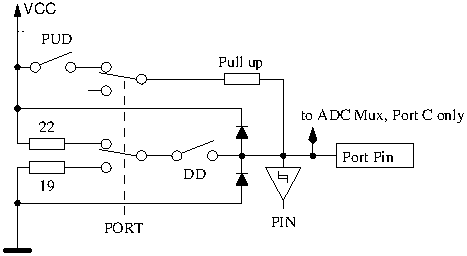
\includegraphics[width=.8\textwidth]{../FIG/port.pdf}
\caption{Zjednodušené schéma každého pinu ATmega portu}
\label{fig:port}
\end{figure}

Každý ze tří zkušebních pinů vašeho testeru se skládá ze tří pinů ATmega,
který je znázorněn na zjednodušeném schéma zkušebního čepu TP2 (prostřední ze tří pinů) na obrázku~\ref{fig:terminal}.

\begin{figure}[H]
\centering
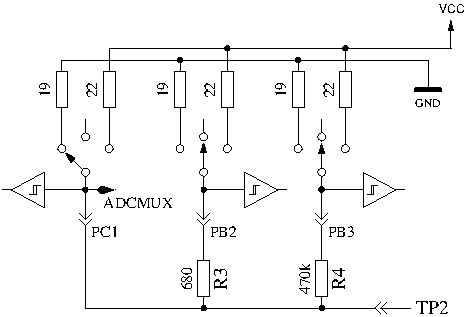
\includegraphics[width=.8\textwidth]{../FIG/terminal.pdf}
\caption{Zjednodušené schéma zapojení zkušebního pinu TP2}
\label{fig:terminal}
\end{figure}

Každý zkušební pin (měřící port) lze použít jako digitální nebo analogový vstup.
Tato schopnost měření je nezávislá na použití portu jako výstupu.
Každý zkušební pin může být použit jako výstup a připojen v tomto stavu k GND (\(0V\)) nebo VCC (\(5V\)),
nebo může být připojen buď k GND nebo VCC pomocí odporů (\(680\Omega\) nebo \(470k\Omega\)).
Tabulka \ref{tab:case} zobrazuje všechny možnosti měření.
Všimněte si, že pozitivní stav je dosažen připojením přímo k VCC (Port C) nebo
připojením k rezistoru \(680\Omega\) s VCC (Port B).
Stejná možnost má negativní stav zkušebního kolíku na straně GND.
Stav testu znamená, že pin může být otevřený (vstup) připojen pomocí odporu \(470k\Omega\) s VCC nebo GND,
nebo pin může být připojen k VCC nebo GND přes \(680\Omega\)-odpor.

\begin{table}[H]
  \begin{center}
    \begin{tabular}{| l | c | c | c |}
    \hline
      & Stav Pin 1 & Stav Pin 2 & Stav Pin 3 \\
    \hline
   1. & positivní    &  negativní   &  test \\
   2. & positivní    &  test      & negativní \\
   3. & test       &  negativní   & positivní \\
   4. & test       &  positivní   & negativní \\
   5. & negativní    &  test      & positivní \\
   6. & negativní    &  positivní   &  test  \\
    \hline
    \end{tabular}
  \end{center}
  \caption{všechny možnosti měření}
  \label{tab:case} 
\end{table}

Jakmile je nakonfigurováno měření kondenzátoru testerem,  pokusí se přístroj nejprve
k vybíjení kondenzátorů na všech připojovacích kolících.
Pokud to nefunguje, to znamená zbytkové napětí je příliš vysoké, bude vybíjení
po cca 12 sekundách přerušeno se zprávou ,,Cell!''.

To se může stát i v případě když není žádný kondenzátor připojen.

Příčinou může v tomto případě být, že je mezní napětí výboje pro tento
ATmega příliš nízké.\\ Pomocí makefile volby CAP\_EMPTY\_LEVEL, můžete ale zvolit vyšší zbytkové napětí.


 %\newpage
\section{Измерение полупроводниковых элементов}
Исследование элемента необходимо начинать с обесточенным управляющим
выводом (третий вывод, назван TriStatePin). TriStatePin исследуемого
элемента во время испытания является  базовым или отправным. Один
испытательный вывод выбран положительной стороной элемента и
подключен непосредственно к VCC. Другой испытательный вывод выбран
отрицательной стороной элемента.
Отрицательная сторона подсоединена через резистор \(680~\Omega\) к GND.
Состояние полевых транзисторов зависит
от напряжения на затворе. Сначала, TriStatePin на \(5~ms\) подключается
через резистор \(680~\Omega\) Ом к GND и измеряется напряжение на отрицательной
стороне. Далее TriStatePin переключается на Ввод (высокое полное
входное сопротивление) и снова измеряется напряжение отрицательного
испытательного вывода. Затем предполагаемый затвор соединяется через
резистор \(680~\Omega\) на \(5~ms\) к VCC и снова измеряется напряжение на
отрицательной  стороне. Если измеренное напряжение ниже первого
результата измерения, то эта схема будет предполагаться, как
правильная. Затем напряжение снова измеряется с обесточенным TriStatePin.\\

Если напряжение отрицательного испытательного вывода с фиксированным 
напряжением TriStatePin выше чем \(115~mV\), а с обесточенным TriStatePin 
не ниже \(100~mV\), предполагается, что это обеднённый транзистор.\\

У биполярных транзисторов, имеющих повышенный обратный ток коллектора,
он значительно повышается в режиме с обесточенной базой.\\

При проверке с обоими напряжениями можно избежать неправильного
обнаружения некоторых германиевых транзисторов с более высоким
обратным током коллектора, как обедненных транзисторов (JFET).\\

Далее проводятся дополнительные тесты по определению N-канального JFET
или N D-MOSFET и P-канального JFET или P-D MOSFET. Версии MOSFET
могут быть определены по отсутствующему току затвора при любом
состоянии TriStatePin.\\

Чтобы получить параметры FET обеднённого типа, их измеряют с резистором \(680~\Omega\) в истоке, 
как показано на рисунке \ref{fig:JFETcd} . Это измерение делается вместо обычного измерения тока 
удерживания затвора на уровне истока, потому, что \(I_\mathrm{DSS}\) FET транзистора часто не может 
быть достигнуто из-за относительно высокого сопротивления резистора \(680~\Omega\).

\begin{figure}[H]
\centering
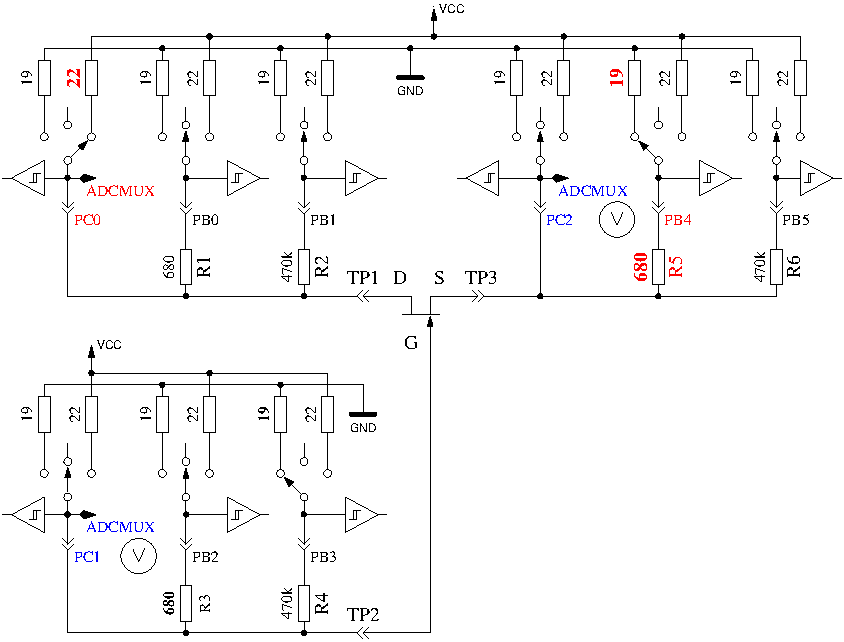
\includegraphics[width=.8\textwidth]{../FIG/JFETcd.pdf}
\caption{Измерение напряжения затвор-исток и тока истока N-JFET транзистора }
\label{fig:JFETcd}
\end{figure}

Если у элемента нет тока между положительным и отрицательным испытательными выводами без сигнала на TristatePin, 
то переходим к тестам определения, описанным в  разделе \ref{sec:pnp}.
Если ток был обнаружен, то следующий тест описан в \ref{sec:diode} о диодах.

\subsection{Измерение P-N-P транзистора или P-Channel-MOSFET}
\label{sec:pnp}
Сначала измеряют коэффициент усиления предполагаемого P-N-P транзистора в схеме с общим коллектором 
(эмиттерный повторитель). Схема измерения показана на рисунке \ref{fig:pnpcc}.
Если напряжение базы (\(UB\)) измеренное с резистором \(680~\Omega\),  выше \(9~mV\), то коэффициент 
усиления вычисляется по формуле \(hFE = \frac{UE-UB}{UB}\).
Напряжение \(UE\) это разность между напряжением на эмиттере и VCC. Различие между резисторами \(22~\Omega\) 
и \(19~\Omega\) не учитывается. Если напряжение \(UB\) ниже \(10~mV\), измерение делают с резистором \(470~k\Omega\) 
в базе. В этом случае коэффициент  
усиления вычисляется по формуле \(hFE = \frac{UE \cdot 470000}{UB \cdot (680+22)}\).

\begin{figure}[H]
\centering
 \begin{overpic}[width=1.\textwidth]{../FIG/PNPcc.pdf}
  \color{black}
  \put(55,20){\makebox(0,0)[lb]{\footnotesize {\textcolor{green}{зеленым} switch state is used,}}}  
  \put(55,17){\makebox(0,0)[lb]{\footnotesize {if Voltage at PC1 is \textless~ 10mV!}}}      
 \end{overpic}
\caption{Измерение hFE P-N-P транзистора в схеме с общим коллектором }
\label{fig:pnpcc}
\end{figure}

Затем делают тесты для предполагаемого P-N-P транзистора в схеме с общим эмиттером. Положительная сторона 
элемента теперь подключена прямо с VCC, отрицательная сторона через резистор \(680~\Omega\) подключена к GND, 
как показано на рисунке \ref{fig:pnpce}. 
Если на отрицательной стороне элемента есть напряжение выше \(3,4~V\), когда базовый резистор \(680~\Omega\) 
подключен к GND, значит этот элемент или P-N-P транзистор или P канальный FET. Какой из них - может быть легко 
установлено по напряжению базы. Если напряжение базы больше \(0,97~V\), это должен быть P-N-P транзистор. Для того, 
чтобы измерить коэффициент усиления, в цепь базы вместо резистора \(680~\Omega\) включается резистор \(470~k\Omega\).
Коэффициент усиления вычисляется по формуле \(hFE = \frac{(UC-UC0) \cdot 470000}{UB \cdot (680+19)}\) .
Напряжение UC0 является напряжением на коллекторном резисторе без базового тока. Как предполагается, правильным 
является более высокий коэффициент усиления, определенный первым или вторым способом. В версии 1.08k коэффициент 
усиления в схеме с общим эмиттером определяется только для микроконтроллеров ATmega328. Для других микроконтроллеров 
используется только схема с общим коллектором.\\

Значения, найденные для P-N-P транзистора, действительны только, если сделаны дополнительные измерения. Чтобы 
предотвратить обнаружение P-N-P транзистора в инверсном включении (коллектор с эмиттером поменяны местами), 
измерение с более высоким коэффициентом усиления считается правильным. 
Если напряжение базы ниже, чем \(0,97~V\), то это должен быть P-E-MOS. В этом случае пороговое напряжение затвора 
измеряется при плавном переключении затвора с резистором \(470~k\Omega\) от VCC до GND, ожидая на цифровом входе 
изменения  сигнала  стока, и затем, считывается напряжение затвора.

\begin{figure}[H]
\centering
 \begin{overpic}[width=1.\textwidth]{../FIG/PNPce.pdf}
  \color{black}
  \put(55,21){\makebox(0,0)[lb]{\footnotesize {The black state is used for Test!}}}  
  \put(55,17){\makebox(0,0)[lb]{\footnotesize {\textcolor{green}{зеленым} state is used for current}}} 
  \put(55,13){\makebox(0,0)[lb]{\footnotesize {gamplification factor hFE!}}}      
 \end{overpic}
\caption{Испытание и измерение hFE P-N-P транзистора в схеме с общим эмиттером }
\label{fig:pnpce}
\end{figure}

\subsection{Измерение N-P-N транзистора или N-Channel-MOSFET}
Измерение N-P-N транзистора начинается таким же образом, как и P-N-P транзистора, с измерения коэффициента усиления 
в схеме с общим коллектором.
Первое измерение сделано с резистором в цепи базы \(680~\Omega\) подключенным к VCC. Если напряжение на резисторе в 
цепи базы слишком низко, вместо \(680~\Omega\) берётся резистор \(470~k\Omega\).
Тогда измерение продолжается в схеме с общим эмиттером, как показано на рисунке \ref{fig:npnce}.
Если напряжение коллектора ниже \(1,6~V\) и резистор в цепи базы \(680~\Omega\) соединён с VCC, то это может быть N-P-N 
транзистор, N-канальный MOSFET или тиристор/симистор. Тиристор или симистор могут быть идентифицированы двумя 
простыми тестами. Если резистор на управляющем выводе, соединённый в течение \(10~ms\) с GND обесточить, ток в аноде 
должен остаться. Если резистор анода кратковременно подключить к GND и, затем, повторно подключить к VCC, тиристор 
не должен снова включиться (нет тока). Имейте в виду, что Тестер может проверять только маломощные тиристоры, потому 
что ток удержания может достигать только \(6~mA\). Если оба теста свидетельствуют о тиристоре, то необходимо сделать 
тесты с обратной полярностью, чтобы исключить или подтвердить симистор. 
\begin{figure}[H]
\centering
 \begin{overpic}[width=1.\textwidth]{../FIG/NPNce.pdf}
  \color{black}
  \put(55,23){\makebox(0,0)[lb]{\footnotesize {The black state is used for Test!}}}  
  \put(55,19){\makebox(0,0)[lb]{\footnotesize {\textcolor{green}{зеленым} state is used for current}}} 
  \put(55,15){\makebox(0,0)[lb]{\footnotesize {amplification factor hFE!}}}      
 \end{overpic}
\caption{Испытание и измерение hFE N-P-N транзистора в схеме с общим эмиттером }
\label{fig:npnce}
\end{figure}
Если ни тиристор, ни симистор не были подтверждены, то это может быть N-P-N транзистор или N канальный E-MOSFET. 
Базовое напряжение N-P-N транзистора будет близко к напряжению эмиттера, таким образом, этот тип может быть 
идентифицирован определенно. Коэффициент усиления в схеме с общим эмиттером вычисляется по формуле 
\(hFE = \frac{(VCC-UC-UC0)\cdot 470000}{(VCC-UB)\cdot (680+22)}\).
Если напряжение базы или затвора повышенные, то в этой цепи тока нет или он мал, значит, элемент будет N-канальным  
E-MOS (MOSFET обогащённый). В этом случае пороговое напряжение измеряется при плавном переключении затвора с 
резистором \(470~k\Omega\) от VCC до GND, ожидая на цифровом входе изменения сигнала стока, и затем считывается 
напряжение затвора. Это измерение делается 11 раз с накоплением результатов АЦП, как показано на 
рисунке~\ref{fig:eleven}.
Результат умножается на 4 и делится на 9, чтобы получить напряжение в \(mV\).
\begin{figure}[H]
\centering
\includegraphics[width=.8\textwidth]{../PNG/IRFU120gate.png}
\caption{Измерение порогового напряжения N-канального MOSFET}
\label{fig:eleven}
\end{figure}

\subsection{Упрощенная блок-схема тестирования транзисторов}

\begin{figure}[H]
\centering
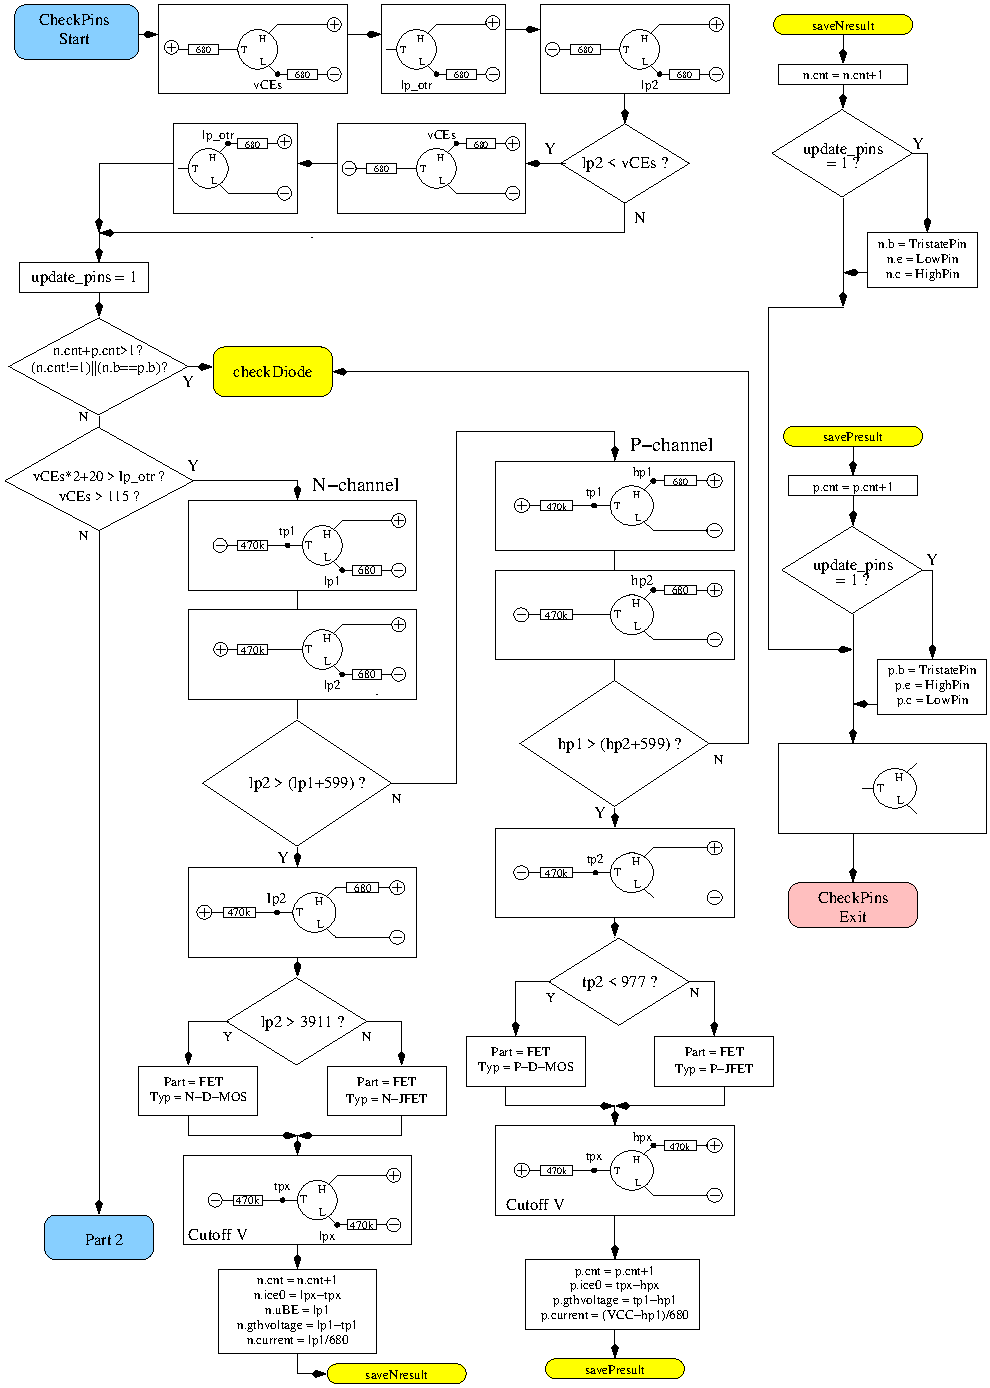
\includegraphics[width=.95\textwidth]{../FIG/CheckSemi1.pdf}
\caption{Блок-схема тестирования транзисторов. Часть 1: JFET и D-MOS}
\label{fig:ChkSemi1}
\end{figure}

\begin{figure}[H]
\centering
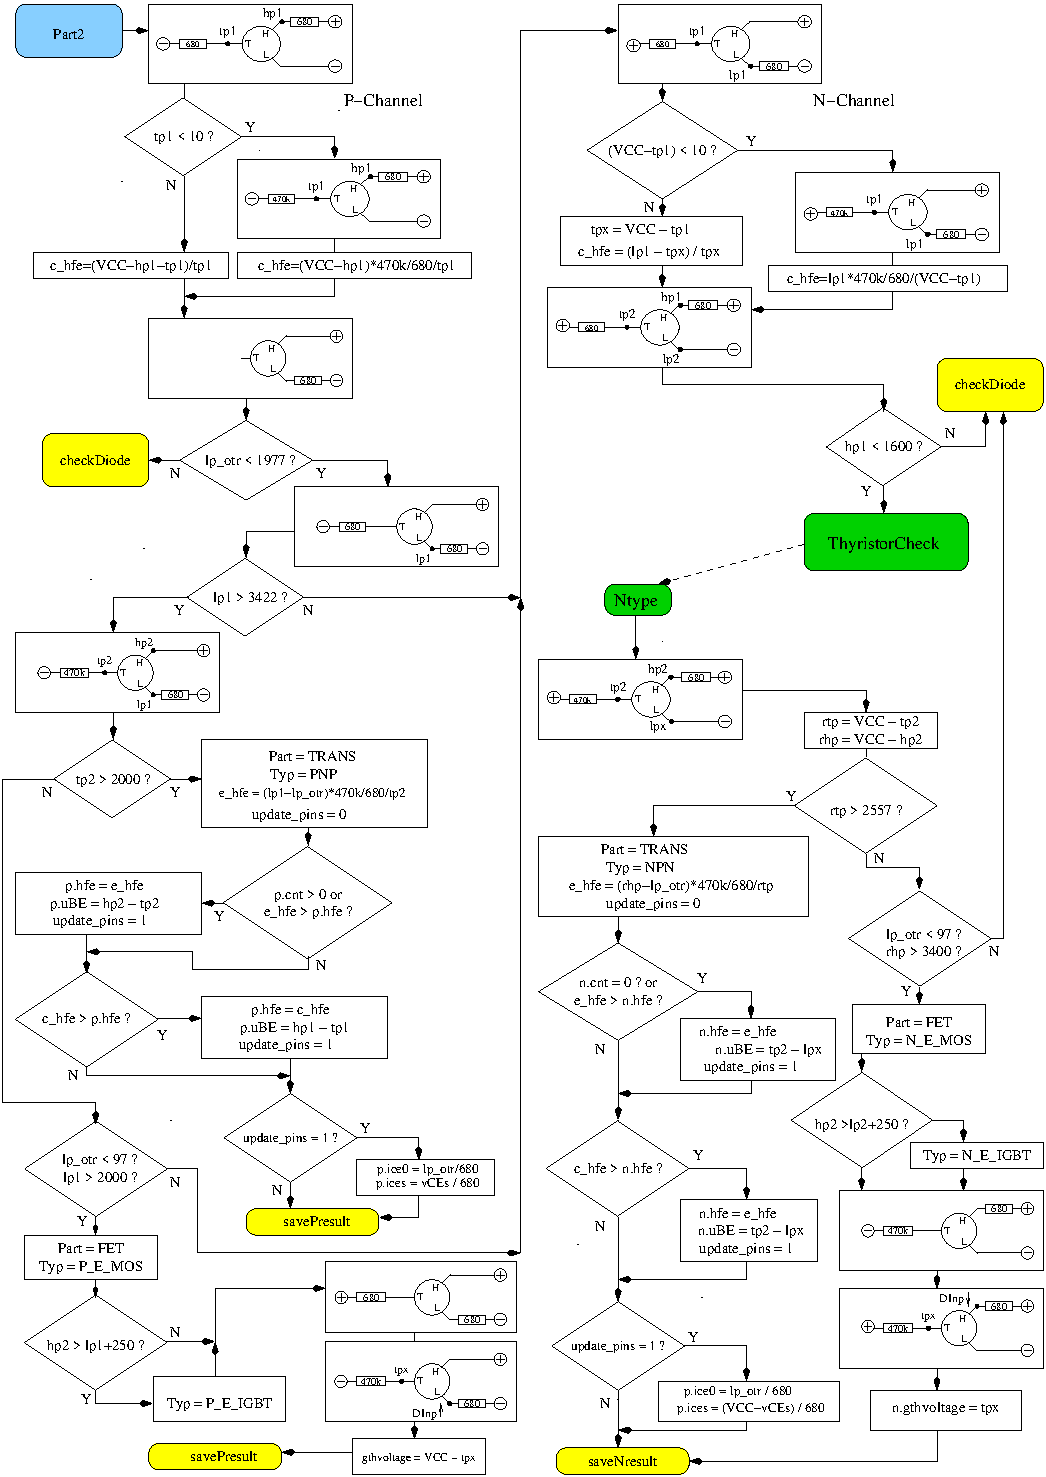
\includegraphics[width=.95\textwidth]{../FIG/CheckSemi2.pdf}
\caption{Блок-схема тестирования транзисторов. Часть 2: BJT и E-MOS}
\label{fig:ChkSemi2}
\end{figure}

\begin{figure}[H]
\centering
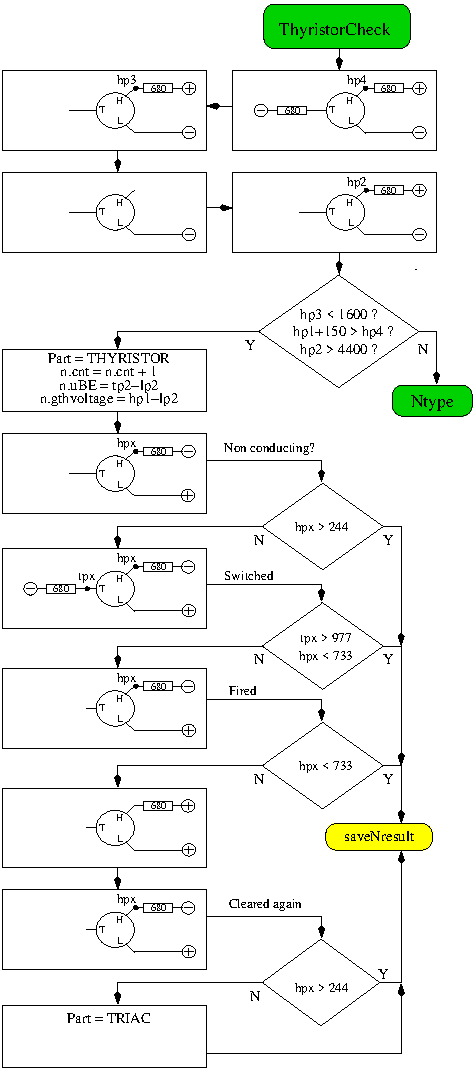
\includegraphics[width=.95\textwidth]{../FIG/CheckSemi3.pdf}
\caption{Блок-схема тестирования транзисторов. Часть 3: Тиристор и симистор}
\label{fig:ChkSemi3}
\end{figure}


\subsection{Измерение диодов}
\label{sec:diode}
Если предварительными тестами будет обнаружен ток, то элемент будет опознан как диод. Падение напряжения с 
резистором \(680~\Omega\) должно быть между \(0,15~V\) и \(4,64~V\). Падение   напряжения с резистором \(680~\Omega\) 
должно быть в 1.125 раза больше падения напряжение с резистором \(470~k\Omega\) и падение  напряжения с 
резистором \(470~k\Omega\) должно быть в 16 раз больше, 
чем падение  напряжения с резистором \(680~\Omega\). Дополнительно: при возобновлении измерения с 
резистором \(470~k\Omega\) напряжения должно быть не выше, чем в предыдущем измерении с 
резистором \(680~\Omega\).
Я надеюсь, что этот метод всегда идентифицирует диод. При идентификации двух диодов, включенных встречно-параллельно, 
невозможно определение тока утечки в противоположном направлении. Если обнаружен только одиночный диод, то ток 
утечки в обратном направлении измеряется с резистором \(470~k\Omega\) подключенным к VCC. Разрешение около \(2~nA\).
Если ток  утечки больше \(5,3~\mu A\) (напряжение на резисторе \(470~k\Omega\) составляет больше чем \(2,5~V\)), 
измерение производится с резистором \(680~\Omega\).
В этом случае разрешение только около \(1~\mu A\).
Кроме того, для одиночного диода, может быть измерена ёмкость в обратном направлении.

\subsection{Результаты различных измерений}
Следующие таблицы показывают результаты испытательных исследований с различными микроконтроллерами 
ATmega8, ATmega168, ATmega328.

\begin{table}[H]
  \begin{center}
    \begin{tabular}{| l | c | c | c |}
    \hline
   Тип диода & Mega8@8MHz & Mega168 @8MHz & Mega328 @8MHz \\                
    \hline
    \hline
1N4148     & Diode, 715mV,        & Diode, 718mV,            & Diode, 715mV,           \\
           &               1pF    &               0pF, 2nA   &               1pF, 4nA  \\
    \hline
1N4150     & Diode, 665mV,        & Diode, 672mV,            & Diode, 666V,           \\
           &               1pF    &               1pF, 4nA   &              2pF, 6nA  \\
    \hline
BA157      & Diode, 619mV,        & Diode, 621V,              & Diode, 615mV,            \\
           &               19pF   &              17pF, 12nA   &               18pF, 12nA \\
    \hline
BY398      & Diode, 538mV,        & Diode, 541mV,             & Diode, 537mV,            \\
           &               16pF   &               14pF, 63nA  &               15pF, 63nA \\
    \hline
1N4007     & Diode, 650mV,        & Diode, 655mV,            & Diode, 650mV,           \\
           &               13pF   &               10pF, 6nA  &               13pF, 6nA \\
    \hline
LED green  & Diode, 1,96V, 5pF    & Diode, 1,95V, 4pF   & Diode, 1.95V, 4pF \\
    \hline
ZPD2,7     & 2xDi, 743mV, 2,53V   & 2xDi, 737mV, 2,52V  & 2xDi, 733mV, 2,51V \\
    \hline
BU508A B+E & Diode, 609mV,        & Diode, 611mV,                & Diode, 606mV,              \\
           &               5,15nF &               5,20nF, 0,39uA &               5,25nF, 0,4uA\\
    \hline
BU508A B+C & Diode, 582mV,        & Diode, 586mV,             & Diode, 587mV,            \\
           &               256pF  &               255pF, 21nA &               259pF, 19nA\\
    \hline
AC128 B+E  & Diode, 272mV,        & Diode, 277mV,              & Diode, 273mV,             \\
           &               0pF    &               0pF, 2,2uA   &               0pF, 2,3uA  \\
    \hline
AC128 B+E  &                      &                     & Diode, 349mV,               \\
с охлаждением     &                      &                     &               140pF, 0,57uA \\
    \hline
MBR20100CT & 2xDi, 337mV, 337mV   & 2xDi, 338mV, 338mV  & 2xDi, 336mV, 335mV  \\
    \hline
MBR20100CT & Diode, 337mV,        & Diode, 339mV,             & Diode, 337mV,            \\
           &               345pF  &               351pF, 29nA &               350pF, 25nA\\
    \hline
MBR4045PT  & Diode, 243mV,        & Diode, 233mV,               & Diode, 235mV,              \\
с охлаждением     &               1,80nF &               1,94nF, 1,7uA &               1,95nF, 1,8uA\\
    \hline
SK14       & Diode,    mV,        & Diode,    mV,               & Diode, 263mV,              \\
           &                  0pF &                   pF,    nA &               0pF, 0,57uA\\
    \hline
SK14       & Diode,    mV,        & Diode,    mV,               & Diode, 334mV,              \\
с охлаждением     &                   nF &                   pF,    nA &               88pF, 4nA\\
    \hline
SF38G      & Diode, 519mV,        & Diode, 521mV,            & Diode, 516mV,            \\
           &               107pF  &               105pF, 2nA &               106pF, 2nA \\
    \hline
    \end{tabular}
  \end{center}
  \caption{Результаты измерения диодов}
  \label{tab:diodes} 
\end{table}

Измерение обратной ёмкости для двойного диода MBR4045PT возможно только с охлаждением. 
Это вызвано высоким током утечки этого \(40~A\) диода. Также обратная ёмкость перехода база-эмиттер 
германиевого транзистора AC128 может быть измерена только с охлаждением.

\begin{table}[H]
  \begin{center}
    \begin{tabular}{| l | c | c | c | c | c |}
    \hline
             Тип & Тип & Mega8           & Mega328        & Mega328         & Mega328 \\
Транзистора     & пр-ти     & общий         &                & общий         & общий \\
            &     & коллектор      &                & коллектор       & эмиттер \\
    \hline
    \hline
BU508A      & NPN & \(\beta\)=9, 601mV      &  \(\beta\)=9, 597mV    &   \(\beta\)=9, 598mV    & \(\beta\)=4, 484mV \\
    \hline
2N3055      & NPN & \(\beta\)=20, 557mV     &  \(\beta\)=21, 550mV   &   \(\beta\)=21, 550mV   & \(\beta\)=6, 442mV \\
    \hline
BC639       & NPN & \(\beta\)=148, 636mV    &  \(\beta\)=172, 629mV  &   \(\beta\)=172, 629mV  & \(\beta\)=158, 605mV \\
    \hline
BC640       & PNP & \(\beta\)=226, 650mV    &  \(\beta\)=176, 609mV  &   \(\beta\)=171, 655mV  & \(\beta\)=177, 608mV \\
    \hline
BC517       & NPN & \(\beta\)=23,9k, 1,23V  &  \(\beta\)=24,8k, 1,22V&   \(\beta\)=25,1k, 1,22V & \(\beta\)=764, 1,23V \\
    \hline
BC516       & PNP & \(\beta\)=75,9k, 1,21V  &  \(\beta\)=76,2k, 1,20V&   \(\beta\)=76,2k, 1,20V & \(\beta\)=760, 1,23V \\
    \hline
BC546B      & NPN & \(\beta\)=285, 694mV    &  \(\beta\)=427, 687mV  &   \(\beta\)=427, 687mV   & \(\beta\)=369, 683mV \\
    \hline
BC556B      & PNP & \(\beta\)=304, 704mV    &  \(\beta\)=254, 668mV  &   \(\beta\)=235, 709mV   & \(\beta\)=255, 668mV \\
    \hline
AC128 (Ge.) & PNP & \(\beta\)=63, 191mV     &  \(\beta\)=59, 191mV   &   \(\beta\)=57, 193mV    & \(\beta\)=43, 117mV \\
    \hline
BUL38D      & NPNp & \(\beta\)=37, 627mV    &  \(\beta\)=41, 617mV  &   \(\beta\)=40, 624mV     & \(\beta\)=36, 562mV \\
parasitic   & PNPn & \(\beta\)=11, 654mV    &  \(\beta\)=81, 543mV  &   \(\beta\)=10, 656mV     & \(\beta\)=83, 541mV \\
    \hline
BRY55/200   & Thyrist. &  0,84V     &  0,81V         &   0,81V          &  0,82V \\
    \hline
MAC97A6     & Triac    &  0,92V     &  0,90V         &   0,90V          &  0,90V \\
    \hline
    \end{tabular}
  \end{center}
  \caption{Результаты измерения биполярных транзисторов}
  \label{tab:bipolar} 
\end{table}

Некоторые результаты значительно отличаются от результатов, полученных в более ранних версиях программного 
обеспечения от Markus F. Например, транзистор Дарлингтона BC517 был измерен более ранним программным 
обеспечением: hFE=797 вместо 77200 и напряжение база-эмиттер = \(1438~mV\). Это вызвано дополнительным измерением 
коэффициента усиления в схеме с общим коллектором. Кроме того, новая версия программного обеспечения показывает 
такой же низкий результат hFE в схеме с общим эмиттером, что можно увидеть в последнем столбце 
таблицы \ref{tab:bipolar}.
Напряжение база-эмиттер измерено как отдельный диод. Теперь напряжение база-эмиттер измеряется при токе измерения 
коэффициента усиления (\(1,20~V\)). NPN-транзистор BUL38D имеет между коллектором и эмиттером встроенный защитный диод, 
который может спровоцировать определение паразитного PNP-транзистора с базой на месте коллектора правильного 
NPN транзистора. С версии программного обеспечения 1.10k оба транзистора обнаруживаются и помечаются добавлением 
символа р. Правильный транзистор будет найден при сравнении ёмкости перехода база - эмиттер. Предполагается, 
что правильный транзистор имеет более высокую ёмкость перехода. Если нажать и удерживать клавишу запуска во время 
вывода результата измерения, то будут показаны параметры паразитного транзистора. Наличие правильного транзистора 
будет отмечено индексом n (PNPn). Паразитный транзистор определяется только с защитным диодом, расположенном на 
том же кристалле, что и правильный транзистор, а не с внешним диодом.\\

Следующая таблица \ref{tab:germanium} показывает результаты измерения для германиевых транзисторов, которые являются 
проблемными из-за температурной зависимости и высокого обратного тока коллектора. Представлены вместе результаты 
оригинальной версии от Markus F. и результаты версии 1.10k. Версия 1.10k для ATmega328 измеряет коэффициент усиления 
в схемах с общим коллектором и общим эмиттером с учетом обратного тока коллектора, и выводит более высокий результат. 
Обратный ток коллектора не учитывался в более ранних версиях программного обеспечения.

\begin{table}[H]
  \begin{center}
    \begin{tabular}{| l | c | c | c |}
    \hline
      Тип & Mega8@1MHz          & Mega168 @8MHz       & Mega328 @8MHz    \\
 транзистора    & Оригинальная вер.    & Версия 1.10k       & Версия 1.10k  \\
            & Markus F.           &                     &        \\
    \hline
    \hline
AC128       & PNP, \(\beta\)=52, 279mV    & PNP, \(\beta\)=59, 184mV    & PNP, \(\beta\)=59, 191mV    \\
    \hline
AC116-65    & PNP, \(\beta\)=505, 378mV   & PNP, \(\beta\)=72, 146mV    & PNP, \(\beta\)=72, 149mV    \\
    \hline
AC116-145   & PNP, \(\beta\)=485, 294mV   & PNP, \(\beta\)=146, 161mV    & PNP, \(\beta\)=146, 163mV   \\
    \hline
AC176-65    & NPN, \(\beta\)=98, 235mV    & NPN, \(\beta\)=58, 94mV    & NPN, \(\beta\)=56, 96mV     \\
    \hline
GC122       & PNP, \(\beta\)=84, 368mV    & PNP, \(\beta\)=55, 117mV    & PNP, \(\beta\)=56, 117mV    \\
    \hline
GC301       & PNP, \(\beta\)=48, 289mV    & PNP, \(\beta\)=39, 184mV    & PNP, \(\beta\)=39, 188mV    \\
    \hline
AD161       & NPN, \(\beta\)=360, 230mV   & NPN, \(\beta\)=296, 126mV   & NPN, \(\beta\)=298, 128mV    \\
    \hline
AD162       & PNP, \(\beta\)=2127, 280mV  & PNP, \(\beta\)=89, 107mV    & PNP, \(\beta\)=89, 107mV    \\
    \hline
    \end{tabular}
  \end{center}
  \caption{Результаты измерений германиевых биполярных транзисторов}
  \label{tab:germanium}
\end{table}

В таблице \ref{tab:mos} показаны результаты измерения некоторых полевых транзисторов. Одним из измеряемых параметров 
E-MOS транзисторов является напряжение затвор-исток, которое замеряется по изменению состояния цифрового входа ATmega, 
подключенному 
к стоку через резистор \(680~\Omega\).
Из-за небольшой ёмкости затвора, напряжение на нем изменяется
очень быстро, что уменьшает точность фиксации этого напряжения. Например, у транзистора BS250 это напряжение
изменялось от \(2,6~V\) до \(2,5~V\), при подключении дополнительного конденсатора ёмкостью
\(10~nF\) параллельно выводам затвор и исток.
Другим измеренным параметром является значение ёмкости затвора.
Емкость затвора измеряется путем переключения вывода истока и затвора на GND.
Доступное напряжение \(5~V\) на затворе тестера является недостаточным для генерации достаточного тока
для некоторых IGBT. Это мешает правильному обнаружению.
В большинстве случаев обнаруживается только защитный диод коллектор-эмиттер.
Источник, примерно, \(3~V\), подключенный к выходу, может решить проблему с обнаружением.
Другой полюс источника должен быть подключен к тестовому выводу (TP) тестера вместо соединения затвора.
При правильной полярности батареи тестер должен обнаружить IGBT.
Отображаемое напряжение переключения затвор-сток должно быть увеличено на величину напряжения батареи,
чтобы получить правильное напряжение переключения.
Для JFET транзисторов в качестве характеристики часто приведен ток Idss,
являющийся током стока при напряжении затвор-исток равном \(0~V\). В данной реализации, однако, ток не может
превышать величины, определенной сопротивлением нагрузки в стоке JFET величиной \(680~\Omega\).
Нагрузочный резистор генерирует обратное напряжение Vgs, которое также отображается на индикаторе.
С нагрузочным резистором \(470~k\Omega\) в цепи истока JFET ток исток-сток будет почти нулевым.
Таким образом, напряжение отсечки Vgs\_off исток-затвор может быть определено достаточно точно,
при условии, что оно не превысит \(5~V\).
С этими двумя рабочими точками мы можем определить ток затвор-исток Igss с почти среднеквадратичной точностью.
Если расчетный ток меньше \(40~mA\), дополнительно проводится измерение без сопротивления в цепи истока.
По более высокому напряжению на выводе истока без резистора мы можем вычислить дополнительное значение тока.
Используя эти результаты измерений, снова вычисляем ток затвор-исток Idss,
при этом он не должен превысить значения \(40~mA\).
Из-за симметричной конструкции транзисторов JFET, невозможно отличить сток от истока.


\begin{table}[H]
  \begin{center}
    \begin{tabular}{| l | c | c | c | c |}
    \hline
 Транзистор  &  Тип    & Mega8@8MHz       & Mega168 @8MHz    & Mega328 @8MHz \\
             &         &                  &                  &               \\
    \hline
    \hline
ZVNL120A     & N-E-MOS & D, 1,6V, 147pF   & D, 1,5V,141pF    & D, 1,5V, 140pF \\
    \hline
IRF530N      & N-E-MOS & D, 3,6V, 1.55nF  & D, 3,6V, 1,54nF  & D, 3,6V, 1,54nF \\
    \hline
BS170        & N-E-MOS & D, 2,6V, 78pF    & D, 2,6V, 68pF    & D, 2,6V, 68pF \\
    \hline
IRL3803      & N-E-MOS & D, 2,3V, 9.81nF  & D, 2,3V, 9,71nF  & D, 2,3V, 9,74nF \\
    \hline
IRFU120N     & N-E-MOS & D, 4,2V, 909pF   & D, 4,2V, 913pF   & D, 4,2V, 911pF \\
    \hline
BUZ71A       & N-E-MOS & D, 3,2V, 714pF   & D, 3,2V, 708pF   & D, 3,2V, 705pF \\
    \hline
ZVP2106A     & P-E-MOS & D, 3,2V, 122pF   & D, 3,2V,115pF    & D, 3,2V, 116pF \\
    \hline
IRF5305      & P-E-MOS & D, 3,6V, 2.22nF  & D, 3,6V, 2,22nF  & D, 3,6V, 2,22nF \\
    \hline
BS250        & P-E-MOS & D, 2,6V, 53pF    & D, 2,6V, 43pF    & D, 2,6V, 44pF \\
    \hline
IRFU9024     & P-E-MOS & D, 3,5V, 937pF   & D, 3,6V, 945pF   & D, 3,5V, 933pF \\
    \hline
J310         & N-JFET  & 3.1mA Vgs=2.2V   & 3.1mA Vgs=2.2V   & 3.1mA Vgs=2.2V \\
Idss=24-60mA &         &                  &                  & Idss=35mA      \\
    \hline
2N5459       & N-JFET  & 2.1mA Vgs=1.5V   & 2.1mA Vgs=1.5V   & 2.1mA Vgs=1.5V \\
Idss=4-16mA &          &                  &                  & Idss=8.2mA     \\
    \hline
BF256C       & N-JFET  & 3.4mA Vgs=2.4V   & 3.4mA Vgs=2.4V   & 3.4mA Vgs=2.4V \\
Idss=11-18mA &         &                  &                  & Idss=14mA      \\
    \hline
BF245A       & N-JFET  & 1.1mA Vgs=.75V   & 1.1mA Vgs=0.75V  & 1.1mA Vgs=0.75V \\
Idss=2-6mA   &         &                  &                  & Idss=3.6mA      \\
    \hline
BF245B       & N-JFET  & 2.5mA Vgs=1.7V   & 2.5mA Vgs=1.7V   & 2.5mA Vgs=1.7V \\
Idss=6-15mA  &         &                  &                  & Idss=10mA      \\
    \hline
BF245C       & N-JFET  & 3.9mA Vgs=2.7V   & 3.9mA Vgs=2.7V   & 3.9mA Vgs=2.7V \\
Idss=12-25mA &         &                  &                  & Idss=17mA    \\
    \hline
J175        & P-JFET   & 3.2mA Vgs=2.2V   & 3.2mA Vgs=2.2V   & 3.2mA Vgs=2.2V \\
Idss=7-60mA &          &                  &                  & Idss=26mA      \\
    \hline
2N5460      & P-JFET   & 0.78mA Vgs=0.54V & 0.77mA Vgs=0.54V & 0.78mA Vgs=0.54V \\
Idss=1-5mA  &          &                  &                  & Idss=2.6mA       \\
    \hline
BSS169      & N-D-MOS   & 2,6mA Vgs=1,8V & D, 2,6mA Vgs=1,8V & D, 2,6mA Vgs=1,8V \\
    \hline
GP07N120    & N-E-IGBT & C=3,81nF Vt=4,2V & C=3,76nF Vt=4,2V & C=3,74nF Vt=4,2V \\
    \hline
G4PC30      & N-E-IGBT &                  &                  & C=2.22nF         \\
с батареей  &          &                  &                  & Vt=2.0V+3.2V \\
    \hline
    \end{tabular}
  \end{center}
  \caption{Результаты измерений МОП-транзисторов}
  \label{tab:mos} 
\end{table}

 %\newpage
\section{��������� ����������}
������ �������� ������� �������� ���������� ������ ��������� � ����� ����������� ����. ��� �� �����  �������� 
����� ������� ���� �� ������ �������� ������ ��������� � ������ ����������� ����. ��������� � ��������������� 
����������� ������������ ������ ��� ����, ����� ���������������� ��������. ���� �������������� ����� ������ 
����������� ������� �������, �� ��� �� ��������.

\subsection{��������� ��������� � ����������� 680 ��}
��������� ������������ ��������� Rx �������������� ����� ��������� � �������������� ������������ ����������
 \(680~\Omega\). ���������� ����� ����� ��������� ��� ������������� ������� 1 (TP1) � 3 (TP3) �������� �� 
��������~\ref{fig:RL1mes} �~\ref{fig:RL2mes} ��� ������ ����� ��������� ���������� ���������.

\begin{figure}[H]
\centering
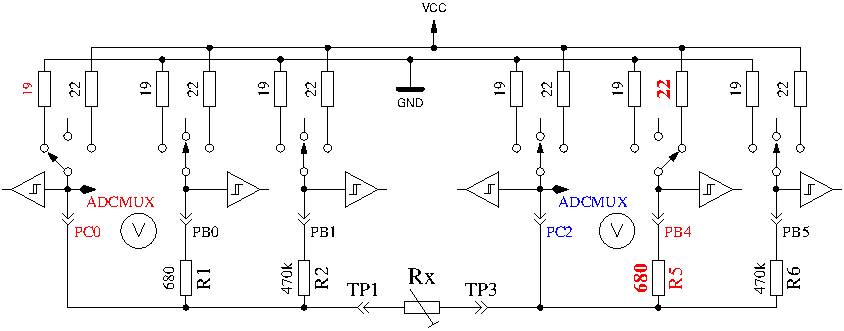
\includegraphics[]{../FIG/ResistormessL1.pdf}
\caption{��������� ���� 1 � ���������� \(680~\Omega\) }
\label{fig:RL1mes}
\end{figure}

\begin{figure}[H]
 \centering
 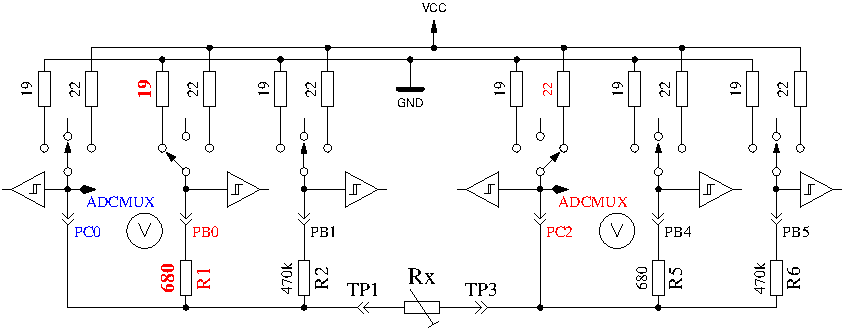
\includegraphics[]{../FIG/ResistormessL2.pdf}
 \caption{��������� ���� 2 � ���������� \(680~\Omega\) }
\label{fig:RL2mes}
\end{figure}


� ����� ������� ���������� ������������� ����� 1, � ������ ������� - ������������� ����� 3. � ����� ���������� 
�� ������, ��� ����� 3 (������ �������) �������� � VCC, ����� 1 (����� �������) �������� � GND. ����������� ����, 
�������� ����� �������� Rx �������� ����������. ��������  ������, ������������� �� �����, �������� ������� ������, 
�������� ������, ������������ � �������� �����, ������������ ����� ������, �������������� ����� - ������. � ����� 
���������� ����� ��������� ��� ������ ���� ����������, ������ ��� ��������� �������� ���������� ����� VCC � GND 
��������� (���� ������������� ��������� ���������� � � ��������� ������). ������ ���������� ���������� �� 
����������, ������ ��� �������� ������������ ���������. 
������ V �� ��������� �������� �����, ������������ ��� ��������� ����������. � ����� ������������� �������� 
��������� Rx ����� ���� ��������� �� ��������� �������� ��������� � ����������� ����������, ���� ��������� 
��������� Rx � \(680~\Omega\) �� ������� ������. ������������� ���������� ���������� �������� �� 
�������~\ref{fig:RLvtot}, ��� �������� ��������� �������� � ��������������� ��������.
\begin{figure}[H]
\centering
% GNUPLOT: LaTeX picture with Postscript
\begingroup
  \makeatletter
  \providecommand\color[2][]{%
    \GenericError{(gnuplot) \space\space\space\@spaces}{%
      Package color not loaded in conjunction with
      terminal option `colourtext'%
    }{See the gnuplot documentation for explanation.%
    }{Either use 'blacktext' in gnuplot or load the package
      color.sty in LaTeX.}%
    \renewcommand\color[2][]{}%
  }%
  \providecommand\includegraphics[2][]{%
    \GenericError{(gnuplot) \space\space\space\@spaces}{%
      Package graphicx or graphics not loaded%
    }{See the gnuplot documentation for explanation.%
    }{The gnuplot epslatex terminal needs graphicx.sty or graphics.sty.}%
    \renewcommand\includegraphics[2][]{}%
  }%
  \providecommand\rotatebox[2]{#2}%
  \@ifundefined{ifGPcolor}{%
    \newif\ifGPcolor
    \GPcolortrue
  }{}%
  \@ifundefined{ifGPblacktext}{%
    \newif\ifGPblacktext
    \GPblacktexttrue
  }{}%
  % define a \g@addto@macro without @ in the name:
  \let\gplgaddtomacro\g@addto@macro
  % define empty templates for all commands taking text:
  \gdef\gplbacktext{}%
  \gdef\gplfronttext{}%
  \makeatother
  \ifGPblacktext
    % no textcolor at all
    \def\colorrgb#1{}%
    \def\colorgray#1{}%
  \else
    % gray or color?
    \ifGPcolor
      \def\colorrgb#1{\color[rgb]{#1}}%
      \def\colorgray#1{\color[gray]{#1}}%
      \expandafter\def\csname LTw\endcsname{\color{white}}%
      \expandafter\def\csname LTb\endcsname{\color{black}}%
      \expandafter\def\csname LTa\endcsname{\color{black}}%
      \expandafter\def\csname LT0\endcsname{\color[rgb]{1,0,0}}%
      \expandafter\def\csname LT1\endcsname{\color[rgb]{0,1,0}}%
      \expandafter\def\csname LT2\endcsname{\color[rgb]{0,0,1}}%
      \expandafter\def\csname LT3\endcsname{\color[rgb]{1,0,1}}%
      \expandafter\def\csname LT4\endcsname{\color[rgb]{0,1,1}}%
      \expandafter\def\csname LT5\endcsname{\color[rgb]{1,1,0}}%
      \expandafter\def\csname LT6\endcsname{\color[rgb]{0,0,0}}%
      \expandafter\def\csname LT7\endcsname{\color[rgb]{1,0.3,0}}%
      \expandafter\def\csname LT8\endcsname{\color[rgb]{0.5,0.5,0.5}}%
    \else
      % gray
      \def\colorrgb#1{\color{black}}%
      \def\colorgray#1{\color[gray]{#1}}%
      \expandafter\def\csname LTw\endcsname{\color{white}}%
      \expandafter\def\csname LTb\endcsname{\color{black}}%
      \expandafter\def\csname LTa\endcsname{\color{black}}%
      \expandafter\def\csname LT0\endcsname{\color{black}}%
      \expandafter\def\csname LT1\endcsname{\color{black}}%
      \expandafter\def\csname LT2\endcsname{\color{black}}%
      \expandafter\def\csname LT3\endcsname{\color{black}}%
      \expandafter\def\csname LT4\endcsname{\color{black}}%
      \expandafter\def\csname LT5\endcsname{\color{black}}%
      \expandafter\def\csname LT6\endcsname{\color{black}}%
      \expandafter\def\csname LT7\endcsname{\color{black}}%
      \expandafter\def\csname LT8\endcsname{\color{black}}%
    \fi
  \fi
    \setlength{\unitlength}{0.0500bp}%
    \ifx\gptboxheight\undefined%
      \newlength{\gptboxheight}%
      \newlength{\gptboxwidth}%
      \newsavebox{\gptboxtext}%
    \fi%
    \setlength{\fboxrule}{0.5pt}%
    \setlength{\fboxsep}{1pt}%
\begin{picture}(7200.00,5040.00)%
    \gplgaddtomacro\gplbacktext{%
      \csname LTb\endcsname%%
      \put(946,704){\makebox(0,0)[r]{\strut{}$0$}}%
      \csname LTb\endcsname%%
      \put(946,1527){\makebox(0,0)[r]{\strut{}$1000$}}%
      \csname LTb\endcsname%%
      \put(946,2350){\makebox(0,0)[r]{\strut{}$2000$}}%
      \csname LTb\endcsname%%
      \put(946,3173){\makebox(0,0)[r]{\strut{}$3000$}}%
      \csname LTb\endcsname%%
      \put(946,3996){\makebox(0,0)[r]{\strut{}$4000$}}%
      \csname LTb\endcsname%%
      \put(946,4819){\makebox(0,0)[r]{\strut{}$5000$}}%
      \csname LTb\endcsname%%
      \put(1078,484){\makebox(0,0){\strut{}0 }}%
      \csname LTb\endcsname%%
      \put(1650,484){\makebox(0,0){\strut{}10k}}%
      \csname LTb\endcsname%%
      \put(2223,484){\makebox(0,0){\strut{}20k}}%
      \csname LTb\endcsname%%
      \put(2795,484){\makebox(0,0){\strut{}30k}}%
      \csname LTb\endcsname%%
      \put(3368,484){\makebox(0,0){\strut{}40k}}%
      \csname LTb\endcsname%%
      \put(3940,484){\makebox(0,0){\strut{}50k}}%
      \csname LTb\endcsname%%
      \put(4513,484){\makebox(0,0){\strut{}60k}}%
      \csname LTb\endcsname%%
      \put(5085,484){\makebox(0,0){\strut{}70k}}%
      \csname LTb\endcsname%%
      \put(5658,484){\makebox(0,0){\strut{}80k}}%
      \csname LTb\endcsname%%
      \put(6230,484){\makebox(0,0){\strut{}90k}}%
      \csname LTb\endcsname%%
      \put(6803,484){\makebox(0,0){\strut{}100k}}%
    }%
    \gplgaddtomacro\gplfronttext{%
      \csname LTb\endcsname%%
      \put(198,2761){\rotatebox{-270}{\makebox(0,0){\strut{}voltage / mV}}}%
      \csname LTb\endcsname%%
      \put(3940,154){\makebox(0,0){\strut{}resistor Rx / Ohm}}%
      \csname LTb\endcsname%%
      \put(3940,4709){\makebox(0,0){\strut{}}}%
      \put(2231,3118){\makebox(0,0){\strut{}}}%
      \csname LTb\endcsname%%
      \put(2530,3118){\makebox(0,0)[r]{\strut{}PC2, type 1}}%
      \csname LTb\endcsname%%
      \put(2530,2898){\makebox(0,0)[r]{\strut{}PC0, type 2}}%
    }%
    \gplbacktext
    \put(0,0){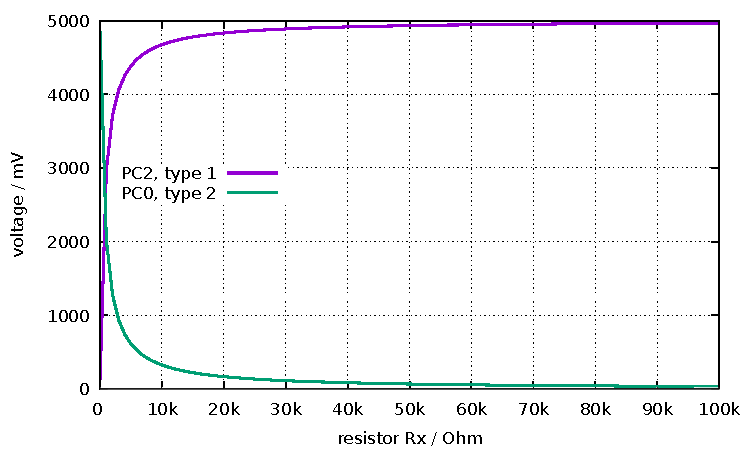
\includegraphics{../GNU/RLvtot}}%
    \gplfronttext
  \end{picture}%
\endgroup

\caption{���������� ��� ���������� ���� 1 � ���� 2 � ���������� \(680~\Omega\) }
\label{fig:RLvtot}
\end{figure}
������  ��������� ���� 1 �������  ��  �������~\ref{fig:RLvlow} � ���������� ��������� ����������� ��� ����� 
�������� ����������. ����� �����, ��� ��� ��������� ������� ��������� �������� ��������� ���� \(2~\Omega\)
���������� ������ ���������� ���, ��� ����������� ���������� \(4,9~mV\) � \(5~V\) ���.  ���� ������ 3 ������� 
��� �� \(0~\Omega\) �� \(2~\Omega\).
����� AUTO\_SCALE\_ADC, ������������� �������� ���, ����� ������ � ���� ������. ��� �� ����� ������� � ���������� 
��������� ����������� ��������� ��������� ���� 2 ������� �� �������~\ref{fig:RLvhigh}.
� ���������, �� �� ����� ������������ ������� ���������� ��� ��� ��������� ����~2 � ���� ���������, ������ ��� 
���������� ������� ������, � � ����������� ATmega ��� ����������������� ����� ���. ��������� � 
����������� \(680~\Omega\) ���������� ��� ��������� ���������� ��������� �� \(20~k\Omega\)
(���������� ���������� ����~2 ����� ���� \(169~mV\)).

��� ����� ������� �������� ����������� ��������� ���������  ���������� � ����������� \(470~k\Omega\). ���� ��� 
����� ��������������� � ���, ��� ��� �� ������ ��� ��������, �� ���������� �������� ����� ��������� ������� � 
�������� �������� ������������� ��������� ��� ����������� �� �������. ���� ������� ����� AUTO\_SCALE\_ADC, � 
���� �� ���������� ����� ����� ��������� ���� \(0,98~V\), ���������� ������� �������� ��������� � ������������� 4 
��� ���� ��������. ������ ���������� �������� ����� ����������� 1. ��� ������� ��� ����, ����� ����������� 
����������� 4 ��� ������� ���������� ����� ���������. ����������� 4 ���� ������ ��� ����������������� ATmega168 
� ATmega328, ��� ATmega8 � �������� �������� ������������ ����� 2, ���� ���������� ���� \(0.98~V\), ������ ��� ������� 
���������� ��� ��� ATmega8 \(2,54~V\) ������ \(1,1~V\) ��� ATmega168 � ATmega328. ��� ATmega168 � ATmega328 ��������� 
���������� �� ���������� ����� ���������, ���� �� ����������� ������� ��������� ��� ���������� ����� �������. 
��� ������������� ����� ������ ������� ������������ ����� �� ������������, ��� ���������, �� ������, � 
������������� ����������� ���� ������� ������� ������������� ����� �������� ���������.


\begin{figure}[H]
  \begin{subfigure}[b]{9cm}
    \centering
    \resizebox{9cm}{!}{% GNUPLOT: LaTeX picture with Postscript
\begingroup
  \makeatletter
  \providecommand\color[2][]{%
    \GenericError{(gnuplot) \space\space\space\@spaces}{%
      Package color not loaded in conjunction with
      terminal option `colourtext'%
    }{See the gnuplot documentation for explanation.%
    }{Either use 'blacktext' in gnuplot or load the package
      color.sty in LaTeX.}%
    \renewcommand\color[2][]{}%
  }%
  \providecommand\includegraphics[2][]{%
    \GenericError{(gnuplot) \space\space\space\@spaces}{%
      Package graphicx or graphics not loaded%
    }{See the gnuplot documentation for explanation.%
    }{The gnuplot epslatex terminal needs graphicx.sty or graphics.sty.}%
    \renewcommand\includegraphics[2][]{}%
  }%
  \providecommand\rotatebox[2]{#2}%
  \@ifundefined{ifGPcolor}{%
    \newif\ifGPcolor
    \GPcolortrue
  }{}%
  \@ifundefined{ifGPblacktext}{%
    \newif\ifGPblacktext
    \GPblacktexttrue
  }{}%
  % define a \g@addto@macro without @ in the name:
  \let\gplgaddtomacro\g@addto@macro
  % define empty templates for all commands taking text:
  \gdef\gplbacktext{}%
  \gdef\gplfronttext{}%
  \makeatother
  \ifGPblacktext
    % no textcolor at all
    \def\colorrgb#1{}%
    \def\colorgray#1{}%
  \else
    % gray or color?
    \ifGPcolor
      \def\colorrgb#1{\color[rgb]{#1}}%
      \def\colorgray#1{\color[gray]{#1}}%
      \expandafter\def\csname LTw\endcsname{\color{white}}%
      \expandafter\def\csname LTb\endcsname{\color{black}}%
      \expandafter\def\csname LTa\endcsname{\color{black}}%
      \expandafter\def\csname LT0\endcsname{\color[rgb]{1,0,0}}%
      \expandafter\def\csname LT1\endcsname{\color[rgb]{0,1,0}}%
      \expandafter\def\csname LT2\endcsname{\color[rgb]{0,0,1}}%
      \expandafter\def\csname LT3\endcsname{\color[rgb]{1,0,1}}%
      \expandafter\def\csname LT4\endcsname{\color[rgb]{0,1,1}}%
      \expandafter\def\csname LT5\endcsname{\color[rgb]{1,1,0}}%
      \expandafter\def\csname LT6\endcsname{\color[rgb]{0,0,0}}%
      \expandafter\def\csname LT7\endcsname{\color[rgb]{1,0.3,0}}%
      \expandafter\def\csname LT8\endcsname{\color[rgb]{0.5,0.5,0.5}}%
    \else
      % gray
      \def\colorrgb#1{\color{black}}%
      \def\colorgray#1{\color[gray]{#1}}%
      \expandafter\def\csname LTw\endcsname{\color{white}}%
      \expandafter\def\csname LTb\endcsname{\color{black}}%
      \expandafter\def\csname LTa\endcsname{\color{black}}%
      \expandafter\def\csname LT0\endcsname{\color{black}}%
      \expandafter\def\csname LT1\endcsname{\color{black}}%
      \expandafter\def\csname LT2\endcsname{\color{black}}%
      \expandafter\def\csname LT3\endcsname{\color{black}}%
      \expandafter\def\csname LT4\endcsname{\color{black}}%
      \expandafter\def\csname LT5\endcsname{\color{black}}%
      \expandafter\def\csname LT6\endcsname{\color{black}}%
      \expandafter\def\csname LT7\endcsname{\color{black}}%
      \expandafter\def\csname LT8\endcsname{\color{black}}%
    \fi
  \fi
    \setlength{\unitlength}{0.0500bp}%
    \ifx\gptboxheight\undefined%
      \newlength{\gptboxheight}%
      \newlength{\gptboxwidth}%
      \newsavebox{\gptboxtext}%
    \fi%
    \setlength{\fboxrule}{0.5pt}%
    \setlength{\fboxsep}{1pt}%
\begin{picture}(7200.00,5040.00)%
    \gplgaddtomacro\gplbacktext{%
      \csname LTb\endcsname%%
      \put(814,704){\makebox(0,0)[r]{\strut{}$130$}}%
      \csname LTb\endcsname%%
      \put(814,998){\makebox(0,0)[r]{\strut{}$135$}}%
      \csname LTb\endcsname%%
      \put(814,1292){\makebox(0,0)[r]{\strut{}$140$}}%
      \csname LTb\endcsname%%
      \put(814,1586){\makebox(0,0)[r]{\strut{}$145$}}%
      \csname LTb\endcsname%%
      \put(814,1880){\makebox(0,0)[r]{\strut{}$150$}}%
      \csname LTb\endcsname%%
      \put(814,2174){\makebox(0,0)[r]{\strut{}$155$}}%
      \csname LTb\endcsname%%
      \put(814,2468){\makebox(0,0)[r]{\strut{}$160$}}%
      \csname LTb\endcsname%%
      \put(814,2762){\makebox(0,0)[r]{\strut{}$165$}}%
      \csname LTb\endcsname%%
      \put(814,3055){\makebox(0,0)[r]{\strut{}$170$}}%
      \csname LTb\endcsname%%
      \put(814,3349){\makebox(0,0)[r]{\strut{}$175$}}%
      \csname LTb\endcsname%%
      \put(814,3643){\makebox(0,0)[r]{\strut{}$180$}}%
      \csname LTb\endcsname%%
      \put(814,3937){\makebox(0,0)[r]{\strut{}$185$}}%
      \csname LTb\endcsname%%
      \put(814,4231){\makebox(0,0)[r]{\strut{}$190$}}%
      \csname LTb\endcsname%%
      \put(814,4525){\makebox(0,0)[r]{\strut{}$195$}}%
      \csname LTb\endcsname%%
      \put(814,4819){\makebox(0,0)[r]{\strut{}$200$}}%
      \csname LTb\endcsname%%
      \put(946,484){\makebox(0,0){\strut{}$0$}}%
      \csname LTb\endcsname%%
      \put(1532,484){\makebox(0,0){\strut{}$1$}}%
      \csname LTb\endcsname%%
      \put(2117,484){\makebox(0,0){\strut{}$2$}}%
      \csname LTb\endcsname%%
      \put(2703,484){\makebox(0,0){\strut{}$3$}}%
      \csname LTb\endcsname%%
      \put(3289,484){\makebox(0,0){\strut{}$4$}}%
      \csname LTb\endcsname%%
      \put(3875,484){\makebox(0,0){\strut{}$5$}}%
      \csname LTb\endcsname%%
      \put(4460,484){\makebox(0,0){\strut{}$6$}}%
      \csname LTb\endcsname%%
      \put(5046,484){\makebox(0,0){\strut{}$7$}}%
      \csname LTb\endcsname%%
      \put(5632,484){\makebox(0,0){\strut{}$8$}}%
      \csname LTb\endcsname%%
      \put(6217,484){\makebox(0,0){\strut{}$9$}}%
      \csname LTb\endcsname%%
      \put(6803,484){\makebox(0,0){\strut{}$10$}}%
    }%
    \gplgaddtomacro\gplfronttext{%
      \csname LTb\endcsname%%
      \put(198,2761){\rotatebox{-270}{\makebox(0,0){\strut{}voltage / mV}}}%
      \csname LTb\endcsname%%
      \put(3874,154){\makebox(0,0){\strut{}resistor Rx / Ohm}}%
      \csname LTb\endcsname%%
      \put(3874,4709){\makebox(0,0){\strut{}}}%
      \put(5517,4646){\makebox(0,0){\strut{}}}%
      \csname LTb\endcsname%%
      \put(5816,4646){\makebox(0,0)[r]{\strut{}PC2, type 1}}%
    }%
    \gplbacktext
    \put(0,0){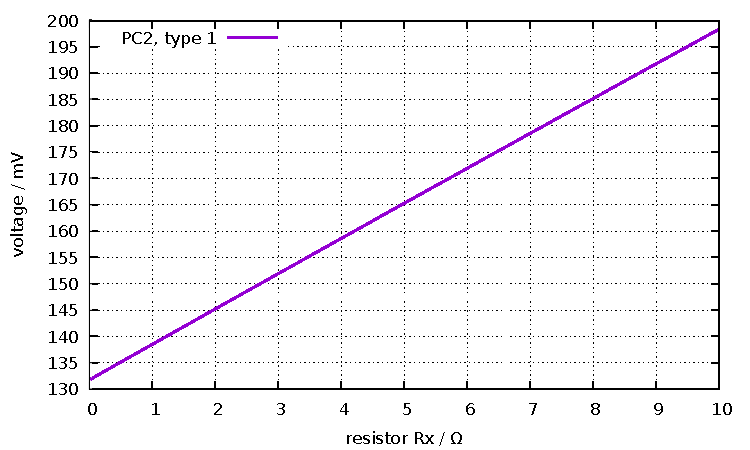
\includegraphics{../GNU/RLvlow}}%
    \gplfronttext
  \end{picture}%
\endgroup
}
    \caption{��������� ���� 1}
    \label{fig:RLvlow}
  \end{subfigure}
  ~
  \begin{subfigure}[b]{9cm}
    \centering
    \resizebox{9cm}{!}{% GNUPLOT: LaTeX picture with Postscript
\begingroup
  \makeatletter
  \providecommand\color[2][]{%
    \GenericError{(gnuplot) \space\space\space\@spaces}{%
      Package color not loaded in conjunction with
      terminal option `colourtext'%
    }{See the gnuplot documentation for explanation.%
    }{Either use 'blacktext' in gnuplot or load the package
      color.sty in LaTeX.}%
    \renewcommand\color[2][]{}%
  }%
  \providecommand\includegraphics[2][]{%
    \GenericError{(gnuplot) \space\space\space\@spaces}{%
      Package graphicx or graphics not loaded%
    }{See the gnuplot documentation for explanation.%
    }{The gnuplot epslatex terminal needs graphicx.sty or graphics.sty.}%
    \renewcommand\includegraphics[2][]{}%
  }%
  \providecommand\rotatebox[2]{#2}%
  \@ifundefined{ifGPcolor}{%
    \newif\ifGPcolor
    \GPcolortrue
  }{}%
  \@ifundefined{ifGPblacktext}{%
    \newif\ifGPblacktext
    \GPblacktexttrue
  }{}%
  % define a \g@addto@macro without @ in the name:
  \let\gplgaddtomacro\g@addto@macro
  % define empty templates for all commands taking text:
  \gdef\gplbacktext{}%
  \gdef\gplfronttext{}%
  \makeatother
  \ifGPblacktext
    % no textcolor at all
    \def\colorrgb#1{}%
    \def\colorgray#1{}%
  \else
    % gray or color?
    \ifGPcolor
      \def\colorrgb#1{\color[rgb]{#1}}%
      \def\colorgray#1{\color[gray]{#1}}%
      \expandafter\def\csname LTw\endcsname{\color{white}}%
      \expandafter\def\csname LTb\endcsname{\color{black}}%
      \expandafter\def\csname LTa\endcsname{\color{black}}%
      \expandafter\def\csname LT0\endcsname{\color[rgb]{1,0,0}}%
      \expandafter\def\csname LT1\endcsname{\color[rgb]{0,1,0}}%
      \expandafter\def\csname LT2\endcsname{\color[rgb]{0,0,1}}%
      \expandafter\def\csname LT3\endcsname{\color[rgb]{1,0,1}}%
      \expandafter\def\csname LT4\endcsname{\color[rgb]{0,1,1}}%
      \expandafter\def\csname LT5\endcsname{\color[rgb]{1,1,0}}%
      \expandafter\def\csname LT6\endcsname{\color[rgb]{0,0,0}}%
      \expandafter\def\csname LT7\endcsname{\color[rgb]{1,0.3,0}}%
      \expandafter\def\csname LT8\endcsname{\color[rgb]{0.5,0.5,0.5}}%
    \else
      % gray
      \def\colorrgb#1{\color{black}}%
      \def\colorgray#1{\color[gray]{#1}}%
      \expandafter\def\csname LTw\endcsname{\color{white}}%
      \expandafter\def\csname LTb\endcsname{\color{black}}%
      \expandafter\def\csname LTa\endcsname{\color{black}}%
      \expandafter\def\csname LT0\endcsname{\color{black}}%
      \expandafter\def\csname LT1\endcsname{\color{black}}%
      \expandafter\def\csname LT2\endcsname{\color{black}}%
      \expandafter\def\csname LT3\endcsname{\color{black}}%
      \expandafter\def\csname LT4\endcsname{\color{black}}%
      \expandafter\def\csname LT5\endcsname{\color{black}}%
      \expandafter\def\csname LT6\endcsname{\color{black}}%
      \expandafter\def\csname LT7\endcsname{\color{black}}%
      \expandafter\def\csname LT8\endcsname{\color{black}}%
    \fi
  \fi
    \setlength{\unitlength}{0.0500bp}%
    \ifx\gptboxheight\undefined%
      \newlength{\gptboxheight}%
      \newlength{\gptboxwidth}%
      \newsavebox{\gptboxtext}%
    \fi%
    \setlength{\fboxrule}{0.5pt}%
    \setlength{\fboxsep}{1pt}%
\begin{picture}(7200.00,5040.00)%
    \gplgaddtomacro\gplbacktext{%
      \csname LTb\endcsname%%
      \put(946,704){\makebox(0,0)[r]{\strut{}$4780$}}%
      \csname LTb\endcsname%%
      \put(946,998){\makebox(0,0)[r]{\strut{}$4785$}}%
      \csname LTb\endcsname%%
      \put(946,1292){\makebox(0,0)[r]{\strut{}$4790$}}%
      \csname LTb\endcsname%%
      \put(946,1586){\makebox(0,0)[r]{\strut{}$4795$}}%
      \csname LTb\endcsname%%
      \put(946,1880){\makebox(0,0)[r]{\strut{}$4800$}}%
      \csname LTb\endcsname%%
      \put(946,2174){\makebox(0,0)[r]{\strut{}$4805$}}%
      \csname LTb\endcsname%%
      \put(946,2468){\makebox(0,0)[r]{\strut{}$4810$}}%
      \csname LTb\endcsname%%
      \put(946,2762){\makebox(0,0)[r]{\strut{}$4815$}}%
      \csname LTb\endcsname%%
      \put(946,3055){\makebox(0,0)[r]{\strut{}$4820$}}%
      \csname LTb\endcsname%%
      \put(946,3349){\makebox(0,0)[r]{\strut{}$4825$}}%
      \csname LTb\endcsname%%
      \put(946,3643){\makebox(0,0)[r]{\strut{}$4830$}}%
      \csname LTb\endcsname%%
      \put(946,3937){\makebox(0,0)[r]{\strut{}$4835$}}%
      \csname LTb\endcsname%%
      \put(946,4231){\makebox(0,0)[r]{\strut{}$4840$}}%
      \csname LTb\endcsname%%
      \put(946,4525){\makebox(0,0)[r]{\strut{}$4845$}}%
      \csname LTb\endcsname%%
      \put(946,4819){\makebox(0,0)[r]{\strut{}$4850$}}%
      \csname LTb\endcsname%%
      \put(1078,484){\makebox(0,0){\strut{}$0$}}%
      \csname LTb\endcsname%%
      \put(1651,484){\makebox(0,0){\strut{}$1$}}%
      \csname LTb\endcsname%%
      \put(2223,484){\makebox(0,0){\strut{}$2$}}%
      \csname LTb\endcsname%%
      \put(2796,484){\makebox(0,0){\strut{}$3$}}%
      \csname LTb\endcsname%%
      \put(3368,484){\makebox(0,0){\strut{}$4$}}%
      \csname LTb\endcsname%%
      \put(3941,484){\makebox(0,0){\strut{}$5$}}%
      \csname LTb\endcsname%%
      \put(4513,484){\makebox(0,0){\strut{}$6$}}%
      \csname LTb\endcsname%%
      \put(5086,484){\makebox(0,0){\strut{}$7$}}%
      \csname LTb\endcsname%%
      \put(5658,484){\makebox(0,0){\strut{}$8$}}%
      \csname LTb\endcsname%%
      \put(6231,484){\makebox(0,0){\strut{}$9$}}%
      \csname LTb\endcsname%%
      \put(6803,484){\makebox(0,0){\strut{}$10$}}%
    }%
    \gplgaddtomacro\gplfronttext{%
      \csname LTb\endcsname%%
      \put(198,2761){\rotatebox{-270}{\makebox(0,0){\strut{}voltage / mV}}}%
      \csname LTb\endcsname%%
      \put(3940,154){\makebox(0,0){\strut{}resistor Rx / Ohm}}%
      \csname LTb\endcsname%%
      \put(3940,4709){\makebox(0,0){\strut{}}}%
      \put(132,-110){\makebox(0,0)[l]{\strut{}}}%
      \put(5517,4646){\makebox(0,0){\strut{}}}%
      \csname LTb\endcsname%%
      \put(5816,4646){\makebox(0,0)[r]{\strut{}PC0, type 2}}%
    }%
    \gplbacktext
    \put(0,0){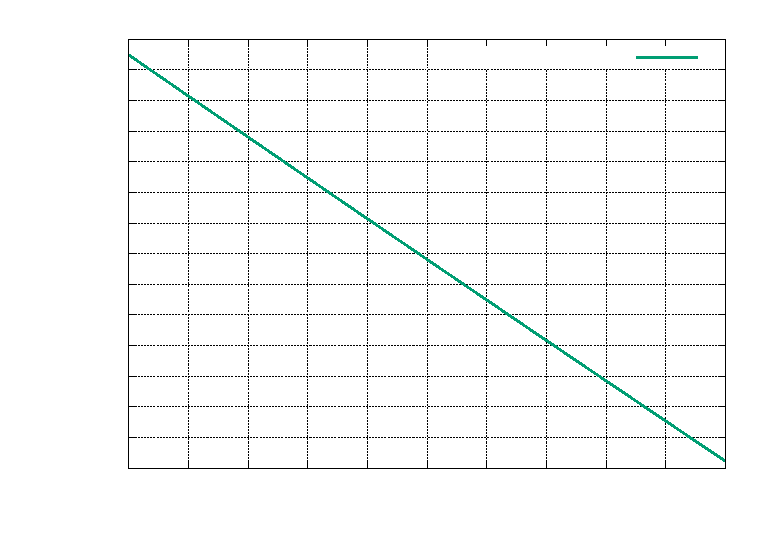
\includegraphics{../GNU/RLvhigh}}%
    \gplfronttext
  \end{picture}%
\endgroup
}
    \caption{��������� ���� 2}
    \label{fig:RLvhigh}
  \end{subfigure}
  \caption{������������� ���������� �� \(0~\Omega\) �� \(10~\Omega\)}
\end{figure}


\subsection{��������� ��������� � ����������� 470 ���}
��������� �������~\ref{fig:RH1mes} � \ref{fig:RH2mes} ���������� �� �� ����� ��������� ��������� � ������������� 
����������� \(470~k\Omega\). ��������� \(470~k\Omega\) ����� ������� ������������ �������� ��������� 
����� \(19~\Omega\) ��� \(22~\Omega\), �������� ���������� ������ �� ����������� ��� ���������� �������� ��������� Rx.

��� ����� ����� ��������� � ����������� \(470~k\Omega\) ���������� ������ ���� ����������, ������ ��� ��� ��������� 
�����, ��� ������� �������� ���������� �� ���������� ���������� ����� ATmega �� ����� ���� �������� (��� � 
���������). ������������� ���������� ���������� �������� �� �������~\ref{fig:RHv} ��� �������� ��������� �������� 
� ��������������� ��������. ������������� ���������� � ���� ��������� ������������� �� \(100~M\Omega\), �� 
����������� �������� ��� ������� ���������� \(60~M\Omega\), ����� ������ ����������, ��� �������� �� ���������. 
���������� ������� ����� ����� ����� ��������� ����� � �������� ���������� � ���� �� ������ ��������������, 
���������� ��� ��������� � ����������� \(680~\Omega\).
��� ���� ����������������� ATmega � ���������, ��� ���������� ���������� � ����������� \(470~k\Omega\) ����� �����, 
���� ����� ��������� ���������� �������� \(350~\Omega\).
���� �������� ����� ���� ��������� ������������ �������� RH\_OFFSET � ����� config.h

\begin{figure}[H]
\centering
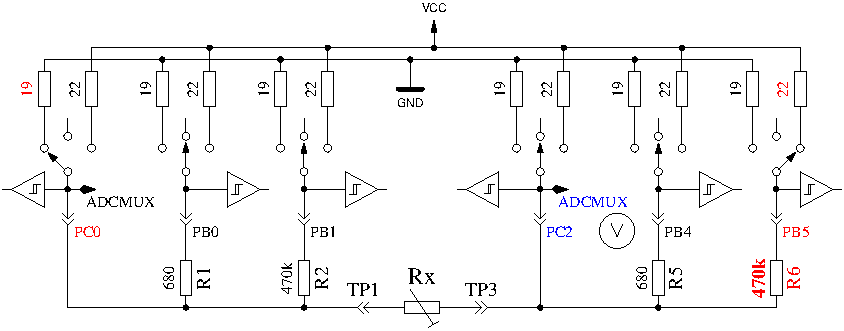
\includegraphics[]{../FIG/ResistormessH1.pdf}
\caption{��������� ���� 3 � ���������� \(470~k\Omega\) }
\label{fig:RH1mes}
\end{figure}

\begin{figure}[H]
 \centering
 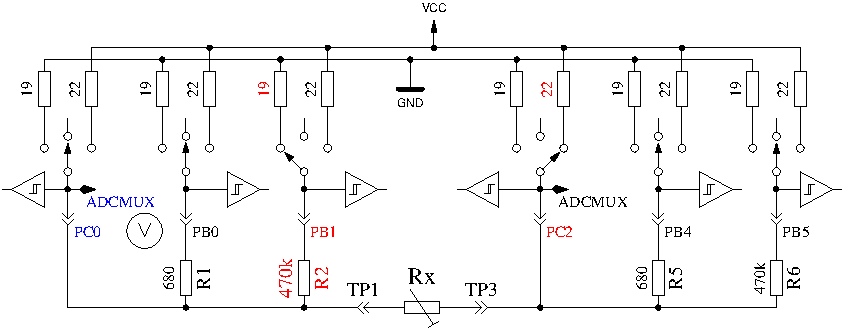
\includegraphics[]{../FIG/ResistormessH2.pdf}
 \caption{��������� ���� 4 � ���������� \(470~k\Omega\) }
\label{fig:RH2mes}
\end{figure}

\begin{figure}[H]
\centering
% GNUPLOT: LaTeX picture with Postscript
\begingroup
  \makeatletter
  \providecommand\color[2][]{%
    \GenericError{(gnuplot) \space\space\space\@spaces}{%
      Package color not loaded in conjunction with
      terminal option `colourtext'%
    }{See the gnuplot documentation for explanation.%
    }{Either use 'blacktext' in gnuplot or load the package
      color.sty in LaTeX.}%
    \renewcommand\color[2][]{}%
  }%
  \providecommand\includegraphics[2][]{%
    \GenericError{(gnuplot) \space\space\space\@spaces}{%
      Package graphicx or graphics not loaded%
    }{See the gnuplot documentation for explanation.%
    }{The gnuplot epslatex terminal needs graphicx.sty or graphics.sty.}%
    \renewcommand\includegraphics[2][]{}%
  }%
  \providecommand\rotatebox[2]{#2}%
  \@ifundefined{ifGPcolor}{%
    \newif\ifGPcolor
    \GPcolortrue
  }{}%
  \@ifundefined{ifGPblacktext}{%
    \newif\ifGPblacktext
    \GPblacktexttrue
  }{}%
  % define a \g@addto@macro without @ in the name:
  \let\gplgaddtomacro\g@addto@macro
  % define empty templates for all commands taking text:
  \gdef\gplbacktext{}%
  \gdef\gplfronttext{}%
  \makeatother
  \ifGPblacktext
    % no textcolor at all
    \def\colorrgb#1{}%
    \def\colorgray#1{}%
  \else
    % gray or color?
    \ifGPcolor
      \def\colorrgb#1{\color[rgb]{#1}}%
      \def\colorgray#1{\color[gray]{#1}}%
      \expandafter\def\csname LTw\endcsname{\color{white}}%
      \expandafter\def\csname LTb\endcsname{\color{black}}%
      \expandafter\def\csname LTa\endcsname{\color{black}}%
      \expandafter\def\csname LT0\endcsname{\color[rgb]{1,0,0}}%
      \expandafter\def\csname LT1\endcsname{\color[rgb]{0,1,0}}%
      \expandafter\def\csname LT2\endcsname{\color[rgb]{0,0,1}}%
      \expandafter\def\csname LT3\endcsname{\color[rgb]{1,0,1}}%
      \expandafter\def\csname LT4\endcsname{\color[rgb]{0,1,1}}%
      \expandafter\def\csname LT5\endcsname{\color[rgb]{1,1,0}}%
      \expandafter\def\csname LT6\endcsname{\color[rgb]{0,0,0}}%
      \expandafter\def\csname LT7\endcsname{\color[rgb]{1,0.3,0}}%
      \expandafter\def\csname LT8\endcsname{\color[rgb]{0.5,0.5,0.5}}%
    \else
      % gray
      \def\colorrgb#1{\color{black}}%
      \def\colorgray#1{\color[gray]{#1}}%
      \expandafter\def\csname LTw\endcsname{\color{white}}%
      \expandafter\def\csname LTb\endcsname{\color{black}}%
      \expandafter\def\csname LTa\endcsname{\color{black}}%
      \expandafter\def\csname LT0\endcsname{\color{black}}%
      \expandafter\def\csname LT1\endcsname{\color{black}}%
      \expandafter\def\csname LT2\endcsname{\color{black}}%
      \expandafter\def\csname LT3\endcsname{\color{black}}%
      \expandafter\def\csname LT4\endcsname{\color{black}}%
      \expandafter\def\csname LT5\endcsname{\color{black}}%
      \expandafter\def\csname LT6\endcsname{\color{black}}%
      \expandafter\def\csname LT7\endcsname{\color{black}}%
      \expandafter\def\csname LT8\endcsname{\color{black}}%
    \fi
  \fi
    \setlength{\unitlength}{0.0500bp}%
    \ifx\gptboxheight\undefined%
      \newlength{\gptboxheight}%
      \newlength{\gptboxwidth}%
      \newsavebox{\gptboxtext}%
    \fi%
    \setlength{\fboxrule}{0.5pt}%
    \setlength{\fboxsep}{1pt}%
\begin{picture}(7200.00,5040.00)%
    \gplgaddtomacro\gplbacktext{%
      \csname LTb\endcsname%%
      \put(946,704){\makebox(0,0)[r]{\strut{}$0$}}%
      \csname LTb\endcsname%%
      \put(946,1527){\makebox(0,0)[r]{\strut{}$1000$}}%
      \csname LTb\endcsname%%
      \put(946,2350){\makebox(0,0)[r]{\strut{}$2000$}}%
      \csname LTb\endcsname%%
      \put(946,3173){\makebox(0,0)[r]{\strut{}$3000$}}%
      \csname LTb\endcsname%%
      \put(946,3996){\makebox(0,0)[r]{\strut{}$4000$}}%
      \csname LTb\endcsname%%
      \put(946,4819){\makebox(0,0)[r]{\strut{}$5000$}}%
      \csname LTb\endcsname%%
      \put(1078,484){\makebox(0,0){\strut{}10k}}%
      \csname LTb\endcsname%%
      \put(2509,484){\makebox(0,0){\strut{}100k}}%
      \csname LTb\endcsname%%
      \put(3940,484){\makebox(0,0){\strut{}1M}}%
      \csname LTb\endcsname%%
      \put(5372,484){\makebox(0,0){\strut{}10M}}%
      \csname LTb\endcsname%%
      \put(6803,484){\makebox(0,0){\strut{}100M}}%
    }%
    \gplgaddtomacro\gplfronttext{%
      \csname LTb\endcsname%%
      \put(198,2761){\rotatebox{-270}{\makebox(0,0){\strut{}voltage / mV}}}%
      \csname LTb\endcsname%%
      \put(3940,154){\makebox(0,0){\strut{}resistor Rx / Ohm}}%
      \csname LTb\endcsname%%
      \put(3940,4709){\makebox(0,0){\strut{}}}%
      \put(5649,2898){\makebox(0,0){\strut{}}}%
      \csname LTb\endcsname%%
      \put(5948,2898){\makebox(0,0)[r]{\strut{}PC2 type 3}}%
      \csname LTb\endcsname%%
      \put(5948,2678){\makebox(0,0)[r]{\strut{}PC0, type 4}}%
    }%
    \gplbacktext
    \put(0,0){\includegraphics{../GNU/RHv}}%
    \gplfronttext
  \end{picture}%
\endgroup

\caption{���������� ��� ���������� ���� 3 � ���� 4 � ���������� \(470~k\Omega\) }
\label{fig:RHv}
\end{figure}

\subsection{���������� ��������� ���������}
�������~\ref{fig:mega8res} ���������� ������������� ����������� ��������� ��������� ����� ATmega8 . ������������� 
��������� ���������� � ������������ ����������� ������������ �� Markus~F. (�Mega8orig�) � ����� ATmega8. �� 
��������~\ref{fig:mega8Ares} � \ref{fig:mega8Lres} �������� ���������� ��������� � ATmega8A � ATmega8L. 
�������~\ref{fig:mega168res} ���������� �� �� ����� ��������� � ATmega168 (Mega168 - ���������� ��� ����� 
AUTOSCALE\_ADC, Mega168as - �� �� ����� ��������� � ������ AUTOSCALE\_ADC). ���������� ATmega168 ���� ����������� 
��������� ���������� � ��������� �� \(20~\Omega\) �� \(20~M\Omega\) � ��������� \(\pm1\%\).
��� ��������� ���� \(100~\Omega\) �� ������ ����� � ����, ��� ����� ������������� ������� ����� ����� �������������. 
����� ������������ �������� ��������������� � ��������� ���������. ���� ��� ����������, ������� �������� 
�������������, ���������� � ������������� ������. ��������, ���� �������� ���������� \(30~\Omega\) � ������ 
���������� �������� \(30,6~\Omega\),
� � ������������ ����� �������� �������� \(0,5~\Omega\), �� ���������� �������� ��������� �������� \(30,1~\Omega\).
��� ������������� ���� \(10~\Omega\) ���� ������  ���������� ��� ������ ������, ��� 1\%!

\begin{figure}[H]
\centering
% GNUPLOT: LaTeX picture with Postscript
\begingroup
  \makeatletter
  \providecommand\color[2][]{%
    \GenericError{(gnuplot) \space\space\space\@spaces}{%
      Package color not loaded in conjunction with
      terminal option `colourtext'%
    }{See the gnuplot documentation for explanation.%
    }{Either use 'blacktext' in gnuplot or load the package
      color.sty in LaTeX.}%
    \renewcommand\color[2][]{}%
  }%
  \providecommand\includegraphics[2][]{%
    \GenericError{(gnuplot) \space\space\space\@spaces}{%
      Package graphicx or graphics not loaded%
    }{See the gnuplot documentation for explanation.%
    }{The gnuplot epslatex terminal needs graphicx.sty or graphics.sty.}%
    \renewcommand\includegraphics[2][]{}%
  }%
  \providecommand\rotatebox[2]{#2}%
  \@ifundefined{ifGPcolor}{%
    \newif\ifGPcolor
    \GPcolortrue
  }{}%
  \@ifundefined{ifGPblacktext}{%
    \newif\ifGPblacktext
    \GPblacktexttrue
  }{}%
  % define a \g@addto@macro without @ in the name:
  \let\gplgaddtomacro\g@addto@macro
  % define empty templates for all commands taking text:
  \gdef\gplbacktext{}%
  \gdef\gplfronttext{}%
  \makeatother
  \ifGPblacktext
    % no textcolor at all
    \def\colorrgb#1{}%
    \def\colorgray#1{}%
  \else
    % gray or color?
    \ifGPcolor
      \def\colorrgb#1{\color[rgb]{#1}}%
      \def\colorgray#1{\color[gray]{#1}}%
      \expandafter\def\csname LTw\endcsname{\color{white}}%
      \expandafter\def\csname LTb\endcsname{\color{black}}%
      \expandafter\def\csname LTa\endcsname{\color{black}}%
      \expandafter\def\csname LT0\endcsname{\color[rgb]{1,0,0}}%
      \expandafter\def\csname LT1\endcsname{\color[rgb]{0,1,0}}%
      \expandafter\def\csname LT2\endcsname{\color[rgb]{0,0,1}}%
      \expandafter\def\csname LT3\endcsname{\color[rgb]{1,0,1}}%
      \expandafter\def\csname LT4\endcsname{\color[rgb]{0,1,1}}%
      \expandafter\def\csname LT5\endcsname{\color[rgb]{1,1,0}}%
      \expandafter\def\csname LT6\endcsname{\color[rgb]{0,0,0}}%
      \expandafter\def\csname LT7\endcsname{\color[rgb]{1,0.3,0}}%
      \expandafter\def\csname LT8\endcsname{\color[rgb]{0.5,0.5,0.5}}%
    \else
      % gray
      \def\colorrgb#1{\color{black}}%
      \def\colorgray#1{\color[gray]{#1}}%
      \expandafter\def\csname LTw\endcsname{\color{white}}%
      \expandafter\def\csname LTb\endcsname{\color{black}}%
      \expandafter\def\csname LTa\endcsname{\color{black}}%
      \expandafter\def\csname LT0\endcsname{\color{black}}%
      \expandafter\def\csname LT1\endcsname{\color{black}}%
      \expandafter\def\csname LT2\endcsname{\color{black}}%
      \expandafter\def\csname LT3\endcsname{\color{black}}%
      \expandafter\def\csname LT4\endcsname{\color{black}}%
      \expandafter\def\csname LT5\endcsname{\color{black}}%
      \expandafter\def\csname LT6\endcsname{\color{black}}%
      \expandafter\def\csname LT7\endcsname{\color{black}}%
      \expandafter\def\csname LT8\endcsname{\color{black}}%
    \fi
  \fi
    \setlength{\unitlength}{0.0500bp}%
    \ifx\gptboxheight\undefined%
      \newlength{\gptboxheight}%
      \newlength{\gptboxwidth}%
      \newsavebox{\gptboxtext}%
    \fi%
    \setlength{\fboxrule}{0.5pt}%
    \setlength{\fboxsep}{1pt}%
\begin{picture}(7200.00,5040.00)%
    \gplgaddtomacro\gplbacktext{%
      \csname LTb\endcsname%%
      \put(682,704){\makebox(0,0)[r]{\strut{}-5}}%
      \csname LTb\endcsname%%
      \put(682,1116){\makebox(0,0)[r]{\strut{}-4}}%
      \csname LTb\endcsname%%
      \put(682,1527){\makebox(0,0)[r]{\strut{}-3}}%
      \csname LTb\endcsname%%
      \put(682,1939){\makebox(0,0)[r]{\strut{}-2}}%
      \csname LTb\endcsname%%
      \put(682,2350){\makebox(0,0)[r]{\strut{}-1}}%
      \csname LTb\endcsname%%
      \put(682,2762){\makebox(0,0)[r]{\strut{} 0}}%
      \csname LTb\endcsname%%
      \put(682,3173){\makebox(0,0)[r]{\strut{} 1}}%
      \csname LTb\endcsname%%
      \put(682,3585){\makebox(0,0)[r]{\strut{} 2}}%
      \csname LTb\endcsname%%
      \put(682,3996){\makebox(0,0)[r]{\strut{} 3}}%
      \csname LTb\endcsname%%
      \put(682,4408){\makebox(0,0)[r]{\strut{} 4}}%
      \csname LTb\endcsname%%
      \put(682,4819){\makebox(0,0)[r]{\strut{} 5}}%
      \csname LTb\endcsname%%
      \put(814,484){\makebox(0,0){\strut{}1 }}%
      \csname LTb\endcsname%%
      \put(1592,484){\makebox(0,0){\strut{}10 }}%
      \csname LTb\endcsname%%
      \put(2370,484){\makebox(0,0){\strut{}100 }}%
      \csname LTb\endcsname%%
      \put(3148,484){\makebox(0,0){\strut{}1k}}%
      \csname LTb\endcsname%%
      \put(3926,484){\makebox(0,0){\strut{}10k}}%
      \csname LTb\endcsname%%
      \put(4703,484){\makebox(0,0){\strut{}100k}}%
      \csname LTb\endcsname%%
      \put(5481,484){\makebox(0,0){\strut{}1M}}%
      \csname LTb\endcsname%%
      \put(6259,484){\makebox(0,0){\strut{}10M}}%
    }%
    \gplgaddtomacro\gplfronttext{%
      \csname LTb\endcsname%%
      \put(198,2761){\rotatebox{-270}{\makebox(0,0){\strut{}Error / Percent}}}%
      \csname LTb\endcsname%%
      \put(3808,154){\makebox(0,0){\strut{}Resistor value / Ohm}}%
      \csname LTb\endcsname%%
      \put(5649,4646){\makebox(0,0){\strut{}}}%
      \csname LTb\endcsname%%
      \put(5816,4646){\makebox(0,0)[r]{\strut{}Mega8-1}}%
      \csname LTb\endcsname%%
      \put(5816,4426){\makebox(0,0)[r]{\strut{}Mega8-2}}%
      \csname LTb\endcsname%%
      \put(5816,4206){\makebox(0,0)[r]{\strut{}Mega8-3}}%
      \csname LTb\endcsname%%
      \put(5816,3986){\makebox(0,0)[r]{\strut{}Mega8orig}}%
    }%
    \gplbacktext
    \put(0,0){\includegraphics{../GNU/Mega8res}}%
    \gplfronttext
  \end{picture}%
\endgroup

\caption{������������� ����������� ��������� ���������� �� ATmega8 }
\label{fig:mega8res}
\end{figure}

\begin{figure}[H]
  \begin{subfigure}[b]{9cm}
    \centering
    \resizebox{9cm}{!}{% GNUPLOT: LaTeX picture with Postscript
\begingroup
  \makeatletter
  \providecommand\color[2][]{%
    \GenericError{(gnuplot) \space\space\space\@spaces}{%
      Package color not loaded in conjunction with
      terminal option `colourtext'%
    }{See the gnuplot documentation for explanation.%
    }{Either use 'blacktext' in gnuplot or load the package
      color.sty in LaTeX.}%
    \renewcommand\color[2][]{}%
  }%
  \providecommand\includegraphics[2][]{%
    \GenericError{(gnuplot) \space\space\space\@spaces}{%
      Package graphicx or graphics not loaded%
    }{See the gnuplot documentation for explanation.%
    }{The gnuplot epslatex terminal needs graphicx.sty or graphics.sty.}%
    \renewcommand\includegraphics[2][]{}%
  }%
  \providecommand\rotatebox[2]{#2}%
  \@ifundefined{ifGPcolor}{%
    \newif\ifGPcolor
    \GPcolortrue
  }{}%
  \@ifundefined{ifGPblacktext}{%
    \newif\ifGPblacktext
    \GPblacktexttrue
  }{}%
  % define a \g@addto@macro without @ in the name:
  \let\gplgaddtomacro\g@addto@macro
  % define empty templates for all commands taking text:
  \gdef\gplbacktext{}%
  \gdef\gplfronttext{}%
  \makeatother
  \ifGPblacktext
    % no textcolor at all
    \def\colorrgb#1{}%
    \def\colorgray#1{}%
  \else
    % gray or color?
    \ifGPcolor
      \def\colorrgb#1{\color[rgb]{#1}}%
      \def\colorgray#1{\color[gray]{#1}}%
      \expandafter\def\csname LTw\endcsname{\color{white}}%
      \expandafter\def\csname LTb\endcsname{\color{black}}%
      \expandafter\def\csname LTa\endcsname{\color{black}}%
      \expandafter\def\csname LT0\endcsname{\color[rgb]{1,0,0}}%
      \expandafter\def\csname LT1\endcsname{\color[rgb]{0,1,0}}%
      \expandafter\def\csname LT2\endcsname{\color[rgb]{0,0,1}}%
      \expandafter\def\csname LT3\endcsname{\color[rgb]{1,0,1}}%
      \expandafter\def\csname LT4\endcsname{\color[rgb]{0,1,1}}%
      \expandafter\def\csname LT5\endcsname{\color[rgb]{1,1,0}}%
      \expandafter\def\csname LT6\endcsname{\color[rgb]{0,0,0}}%
      \expandafter\def\csname LT7\endcsname{\color[rgb]{1,0.3,0}}%
      \expandafter\def\csname LT8\endcsname{\color[rgb]{0.5,0.5,0.5}}%
    \else
      % gray
      \def\colorrgb#1{\color{black}}%
      \def\colorgray#1{\color[gray]{#1}}%
      \expandafter\def\csname LTw\endcsname{\color{white}}%
      \expandafter\def\csname LTb\endcsname{\color{black}}%
      \expandafter\def\csname LTa\endcsname{\color{black}}%
      \expandafter\def\csname LT0\endcsname{\color{black}}%
      \expandafter\def\csname LT1\endcsname{\color{black}}%
      \expandafter\def\csname LT2\endcsname{\color{black}}%
      \expandafter\def\csname LT3\endcsname{\color{black}}%
      \expandafter\def\csname LT4\endcsname{\color{black}}%
      \expandafter\def\csname LT5\endcsname{\color{black}}%
      \expandafter\def\csname LT6\endcsname{\color{black}}%
      \expandafter\def\csname LT7\endcsname{\color{black}}%
      \expandafter\def\csname LT8\endcsname{\color{black}}%
    \fi
  \fi
    \setlength{\unitlength}{0.0500bp}%
    \ifx\gptboxheight\undefined%
      \newlength{\gptboxheight}%
      \newlength{\gptboxwidth}%
      \newsavebox{\gptboxtext}%
    \fi%
    \setlength{\fboxrule}{0.5pt}%
    \setlength{\fboxsep}{1pt}%
\begin{picture}(7200.00,5040.00)%
    \gplgaddtomacro\gplbacktext{%
      \csname LTb\endcsname%%
      \put(682,704){\makebox(0,0)[r]{\strut{}-5}}%
      \csname LTb\endcsname%%
      \put(682,1116){\makebox(0,0)[r]{\strut{}-4}}%
      \csname LTb\endcsname%%
      \put(682,1527){\makebox(0,0)[r]{\strut{}-3}}%
      \csname LTb\endcsname%%
      \put(682,1939){\makebox(0,0)[r]{\strut{}-2}}%
      \csname LTb\endcsname%%
      \put(682,2350){\makebox(0,0)[r]{\strut{}-1}}%
      \csname LTb\endcsname%%
      \put(682,2762){\makebox(0,0)[r]{\strut{} 0}}%
      \csname LTb\endcsname%%
      \put(682,3173){\makebox(0,0)[r]{\strut{} 1}}%
      \csname LTb\endcsname%%
      \put(682,3585){\makebox(0,0)[r]{\strut{} 2}}%
      \csname LTb\endcsname%%
      \put(682,3996){\makebox(0,0)[r]{\strut{} 3}}%
      \csname LTb\endcsname%%
      \put(682,4408){\makebox(0,0)[r]{\strut{} 4}}%
      \csname LTb\endcsname%%
      \put(682,4819){\makebox(0,0)[r]{\strut{} 5}}%
      \csname LTb\endcsname%%
      \put(814,484){\makebox(0,0){\strut{}1 }}%
      \csname LTb\endcsname%%
      \put(1592,484){\makebox(0,0){\strut{}10 }}%
      \csname LTb\endcsname%%
      \put(2370,484){\makebox(0,0){\strut{}100 }}%
      \csname LTb\endcsname%%
      \put(3148,484){\makebox(0,0){\strut{}1k}}%
      \csname LTb\endcsname%%
      \put(3926,484){\makebox(0,0){\strut{}10k}}%
      \csname LTb\endcsname%%
      \put(4703,484){\makebox(0,0){\strut{}100k}}%
      \csname LTb\endcsname%%
      \put(5481,484){\makebox(0,0){\strut{}1M}}%
      \csname LTb\endcsname%%
      \put(6259,484){\makebox(0,0){\strut{}10M}}%
    }%
    \gplgaddtomacro\gplfronttext{%
      \csname LTb\endcsname%%
      \put(198,2761){\rotatebox{-270}{\makebox(0,0){\strut{}Error / Percent}}}%
      \csname LTb\endcsname%%
      \put(3808,154){\makebox(0,0){\strut{}Resistor value / Ohm}}%
      \csname LTb\endcsname%%
      \put(5715,4646){\makebox(0,0){\strut{}}}%
      \csname LTb\endcsname%%
      \put(5816,4646){\makebox(0,0)[r]{\strut{}Mega8A-4}}%
      \csname LTb\endcsname%%
      \put(5816,4426){\makebox(0,0)[r]{\strut{}Mega8A-5}}%
      \csname LTb\endcsname%%
      \put(5816,4206){\makebox(0,0)[r]{\strut{}Mega8A-6}}%
    }%
    \gplbacktext
    \put(0,0){\includegraphics{../GNU/Mega8Ares}}%
    \gplfronttext
  \end{picture}%
\endgroup
}
    \caption{ATmega8A}
    \label{fig:mega8Ares}
  \end{subfigure}
  ~
  \begin{subfigure}[b]{9cm}
    \centering
    \resizebox{9cm}{!}{% GNUPLOT: LaTeX picture with Postscript
\begingroup
  \makeatletter
  \providecommand\color[2][]{%
    \GenericError{(gnuplot) \space\space\space\@spaces}{%
      Package color not loaded in conjunction with
      terminal option `colourtext'%
    }{See the gnuplot documentation for explanation.%
    }{Either use 'blacktext' in gnuplot or load the package
      color.sty in LaTeX.}%
    \renewcommand\color[2][]{}%
  }%
  \providecommand\includegraphics[2][]{%
    \GenericError{(gnuplot) \space\space\space\@spaces}{%
      Package graphicx or graphics not loaded%
    }{See the gnuplot documentation for explanation.%
    }{The gnuplot epslatex terminal needs graphicx.sty or graphics.sty.}%
    \renewcommand\includegraphics[2][]{}%
  }%
  \providecommand\rotatebox[2]{#2}%
  \@ifundefined{ifGPcolor}{%
    \newif\ifGPcolor
    \GPcolortrue
  }{}%
  \@ifundefined{ifGPblacktext}{%
    \newif\ifGPblacktext
    \GPblacktexttrue
  }{}%
  % define a \g@addto@macro without @ in the name:
  \let\gplgaddtomacro\g@addto@macro
  % define empty templates for all commands taking text:
  \gdef\gplbacktext{}%
  \gdef\gplfronttext{}%
  \makeatother
  \ifGPblacktext
    % no textcolor at all
    \def\colorrgb#1{}%
    \def\colorgray#1{}%
  \else
    % gray or color?
    \ifGPcolor
      \def\colorrgb#1{\color[rgb]{#1}}%
      \def\colorgray#1{\color[gray]{#1}}%
      \expandafter\def\csname LTw\endcsname{\color{white}}%
      \expandafter\def\csname LTb\endcsname{\color{black}}%
      \expandafter\def\csname LTa\endcsname{\color{black}}%
      \expandafter\def\csname LT0\endcsname{\color[rgb]{1,0,0}}%
      \expandafter\def\csname LT1\endcsname{\color[rgb]{0,1,0}}%
      \expandafter\def\csname LT2\endcsname{\color[rgb]{0,0,1}}%
      \expandafter\def\csname LT3\endcsname{\color[rgb]{1,0,1}}%
      \expandafter\def\csname LT4\endcsname{\color[rgb]{0,1,1}}%
      \expandafter\def\csname LT5\endcsname{\color[rgb]{1,1,0}}%
      \expandafter\def\csname LT6\endcsname{\color[rgb]{0,0,0}}%
      \expandafter\def\csname LT7\endcsname{\color[rgb]{1,0.3,0}}%
      \expandafter\def\csname LT8\endcsname{\color[rgb]{0.5,0.5,0.5}}%
    \else
      % gray
      \def\colorrgb#1{\color{black}}%
      \def\colorgray#1{\color[gray]{#1}}%
      \expandafter\def\csname LTw\endcsname{\color{white}}%
      \expandafter\def\csname LTb\endcsname{\color{black}}%
      \expandafter\def\csname LTa\endcsname{\color{black}}%
      \expandafter\def\csname LT0\endcsname{\color{black}}%
      \expandafter\def\csname LT1\endcsname{\color{black}}%
      \expandafter\def\csname LT2\endcsname{\color{black}}%
      \expandafter\def\csname LT3\endcsname{\color{black}}%
      \expandafter\def\csname LT4\endcsname{\color{black}}%
      \expandafter\def\csname LT5\endcsname{\color{black}}%
      \expandafter\def\csname LT6\endcsname{\color{black}}%
      \expandafter\def\csname LT7\endcsname{\color{black}}%
      \expandafter\def\csname LT8\endcsname{\color{black}}%
    \fi
  \fi
    \setlength{\unitlength}{0.0500bp}%
    \ifx\gptboxheight\undefined%
      \newlength{\gptboxheight}%
      \newlength{\gptboxwidth}%
      \newsavebox{\gptboxtext}%
    \fi%
    \setlength{\fboxrule}{0.5pt}%
    \setlength{\fboxsep}{1pt}%
\begin{picture}(7200.00,5040.00)%
    \gplgaddtomacro\gplbacktext{%
      \csname LTb\endcsname%%
      \put(682,704){\makebox(0,0)[r]{\strut{}-5}}%
      \csname LTb\endcsname%%
      \put(682,1116){\makebox(0,0)[r]{\strut{}-4}}%
      \csname LTb\endcsname%%
      \put(682,1527){\makebox(0,0)[r]{\strut{}-3}}%
      \csname LTb\endcsname%%
      \put(682,1939){\makebox(0,0)[r]{\strut{}-2}}%
      \csname LTb\endcsname%%
      \put(682,2350){\makebox(0,0)[r]{\strut{}-1}}%
      \csname LTb\endcsname%%
      \put(682,2762){\makebox(0,0)[r]{\strut{} 0}}%
      \csname LTb\endcsname%%
      \put(682,3173){\makebox(0,0)[r]{\strut{} 1}}%
      \csname LTb\endcsname%%
      \put(682,3585){\makebox(0,0)[r]{\strut{} 2}}%
      \csname LTb\endcsname%%
      \put(682,3996){\makebox(0,0)[r]{\strut{} 3}}%
      \csname LTb\endcsname%%
      \put(682,4408){\makebox(0,0)[r]{\strut{} 4}}%
      \csname LTb\endcsname%%
      \put(682,4819){\makebox(0,0)[r]{\strut{} 5}}%
      \csname LTb\endcsname%%
      \put(814,484){\makebox(0,0){\strut{}1 }}%
      \csname LTb\endcsname%%
      \put(1592,484){\makebox(0,0){\strut{}10 }}%
      \csname LTb\endcsname%%
      \put(2370,484){\makebox(0,0){\strut{}100 }}%
      \csname LTb\endcsname%%
      \put(3148,484){\makebox(0,0){\strut{}1k}}%
      \csname LTb\endcsname%%
      \put(3926,484){\makebox(0,0){\strut{}10k}}%
      \csname LTb\endcsname%%
      \put(4703,484){\makebox(0,0){\strut{}100k}}%
      \csname LTb\endcsname%%
      \put(5481,484){\makebox(0,0){\strut{}1M}}%
      \csname LTb\endcsname%%
      \put(6259,484){\makebox(0,0){\strut{}10M}}%
    }%
    \gplgaddtomacro\gplfronttext{%
      \csname LTb\endcsname%%
      \put(198,2761){\rotatebox{-270}{\makebox(0,0){\strut{}Error / Percent}}}%
      \csname LTb\endcsname%%
      \put(3808,154){\makebox(0,0){\strut{}Resistor value / Ohm}}%
      \csname LTb\endcsname%%
      \put(5715,4646){\makebox(0,0){\strut{}}}%
      \csname LTb\endcsname%%
      \put(5816,4646){\makebox(0,0)[r]{\strut{}Mega8L-7}}%
      \csname LTb\endcsname%%
      \put(5816,4426){\makebox(0,0)[r]{\strut{}Mega8L-8}}%
      \csname LTb\endcsname%%
      \put(5816,4206){\makebox(0,0)[r]{\strut{}Mega8L-9}}%
    }%
    \gplbacktext
    \put(0,0){\includegraphics{../GNU/Mega8Lres}}%
    \gplfronttext
  \end{picture}%
\endgroup
}
    \caption{ATmega8L}
    \label{fig:mega8Lres}
  \end{subfigure}
\caption{������������� ����������� ��������� ����������}
\end{figure}


\begin{figure}[H]
\centering
% GNUPLOT: LaTeX picture with Postscript
\begingroup
  \makeatletter
  \providecommand\color[2][]{%
    \GenericError{(gnuplot) \space\space\space\@spaces}{%
      Package color not loaded in conjunction with
      terminal option `colourtext'%
    }{See the gnuplot documentation for explanation.%
    }{Either use 'blacktext' in gnuplot or load the package
      color.sty in LaTeX.}%
    \renewcommand\color[2][]{}%
  }%
  \providecommand\includegraphics[2][]{%
    \GenericError{(gnuplot) \space\space\space\@spaces}{%
      Package graphicx or graphics not loaded%
    }{See the gnuplot documentation for explanation.%
    }{The gnuplot epslatex terminal needs graphicx.sty or graphics.sty.}%
    \renewcommand\includegraphics[2][]{}%
  }%
  \providecommand\rotatebox[2]{#2}%
  \@ifundefined{ifGPcolor}{%
    \newif\ifGPcolor
    \GPcolortrue
  }{}%
  \@ifundefined{ifGPblacktext}{%
    \newif\ifGPblacktext
    \GPblacktexttrue
  }{}%
  % define a \g@addto@macro without @ in the name:
  \let\gplgaddtomacro\g@addto@macro
  % define empty templates for all commands taking text:
  \gdef\gplbacktext{}%
  \gdef\gplfronttext{}%
  \makeatother
  \ifGPblacktext
    % no textcolor at all
    \def\colorrgb#1{}%
    \def\colorgray#1{}%
  \else
    % gray or color?
    \ifGPcolor
      \def\colorrgb#1{\color[rgb]{#1}}%
      \def\colorgray#1{\color[gray]{#1}}%
      \expandafter\def\csname LTw\endcsname{\color{white}}%
      \expandafter\def\csname LTb\endcsname{\color{black}}%
      \expandafter\def\csname LTa\endcsname{\color{black}}%
      \expandafter\def\csname LT0\endcsname{\color[rgb]{1,0,0}}%
      \expandafter\def\csname LT1\endcsname{\color[rgb]{0,1,0}}%
      \expandafter\def\csname LT2\endcsname{\color[rgb]{0,0,1}}%
      \expandafter\def\csname LT3\endcsname{\color[rgb]{1,0,1}}%
      \expandafter\def\csname LT4\endcsname{\color[rgb]{0,1,1}}%
      \expandafter\def\csname LT5\endcsname{\color[rgb]{1,1,0}}%
      \expandafter\def\csname LT6\endcsname{\color[rgb]{0,0,0}}%
      \expandafter\def\csname LT7\endcsname{\color[rgb]{1,0.3,0}}%
      \expandafter\def\csname LT8\endcsname{\color[rgb]{0.5,0.5,0.5}}%
    \else
      % gray
      \def\colorrgb#1{\color{black}}%
      \def\colorgray#1{\color[gray]{#1}}%
      \expandafter\def\csname LTw\endcsname{\color{white}}%
      \expandafter\def\csname LTb\endcsname{\color{black}}%
      \expandafter\def\csname LTa\endcsname{\color{black}}%
      \expandafter\def\csname LT0\endcsname{\color{black}}%
      \expandafter\def\csname LT1\endcsname{\color{black}}%
      \expandafter\def\csname LT2\endcsname{\color{black}}%
      \expandafter\def\csname LT3\endcsname{\color{black}}%
      \expandafter\def\csname LT4\endcsname{\color{black}}%
      \expandafter\def\csname LT5\endcsname{\color{black}}%
      \expandafter\def\csname LT6\endcsname{\color{black}}%
      \expandafter\def\csname LT7\endcsname{\color{black}}%
      \expandafter\def\csname LT8\endcsname{\color{black}}%
    \fi
  \fi
    \setlength{\unitlength}{0.0500bp}%
    \ifx\gptboxheight\undefined%
      \newlength{\gptboxheight}%
      \newlength{\gptboxwidth}%
      \newsavebox{\gptboxtext}%
    \fi%
    \setlength{\fboxrule}{0.5pt}%
    \setlength{\fboxsep}{1pt}%
\begin{picture}(7200.00,5040.00)%
    \gplgaddtomacro\gplbacktext{%
      \csname LTb\endcsname%%
      \put(682,704){\makebox(0,0)[r]{\strut{}-5}}%
      \csname LTb\endcsname%%
      \put(682,1116){\makebox(0,0)[r]{\strut{}-4}}%
      \csname LTb\endcsname%%
      \put(682,1527){\makebox(0,0)[r]{\strut{}-3}}%
      \csname LTb\endcsname%%
      \put(682,1939){\makebox(0,0)[r]{\strut{}-2}}%
      \csname LTb\endcsname%%
      \put(682,2350){\makebox(0,0)[r]{\strut{}-1}}%
      \csname LTb\endcsname%%
      \put(682,2762){\makebox(0,0)[r]{\strut{} 0}}%
      \csname LTb\endcsname%%
      \put(682,3173){\makebox(0,0)[r]{\strut{} 1}}%
      \csname LTb\endcsname%%
      \put(682,3585){\makebox(0,0)[r]{\strut{} 2}}%
      \csname LTb\endcsname%%
      \put(682,3996){\makebox(0,0)[r]{\strut{} 3}}%
      \csname LTb\endcsname%%
      \put(682,4408){\makebox(0,0)[r]{\strut{} 4}}%
      \csname LTb\endcsname%%
      \put(682,4819){\makebox(0,0)[r]{\strut{} 5}}%
      \csname LTb\endcsname%%
      \put(814,484){\makebox(0,0){\strut{}1 }}%
      \csname LTb\endcsname%%
      \put(1592,484){\makebox(0,0){\strut{}10 }}%
      \csname LTb\endcsname%%
      \put(2370,484){\makebox(0,0){\strut{}100 }}%
      \csname LTb\endcsname%%
      \put(3148,484){\makebox(0,0){\strut{}1k}}%
      \csname LTb\endcsname%%
      \put(3926,484){\makebox(0,0){\strut{}10k}}%
      \csname LTb\endcsname%%
      \put(4703,484){\makebox(0,0){\strut{}100k}}%
      \csname LTb\endcsname%%
      \put(5481,484){\makebox(0,0){\strut{}1M}}%
      \csname LTb\endcsname%%
      \put(6259,484){\makebox(0,0){\strut{}10M}}%
    }%
    \gplgaddtomacro\gplfronttext{%
      \csname LTb\endcsname%%
      \put(198,2761){\rotatebox{-270}{\makebox(0,0){\strut{}Error / Percent}}}%
      \csname LTb\endcsname%%
      \put(3808,154){\makebox(0,0){\strut{}Resistor value / Ohm}}%
      \csname LTb\endcsname%%
      \put(5649,4646){\makebox(0,0){\strut{}}}%
      \csname LTb\endcsname%%
      \put(5816,4646){\makebox(0,0)[r]{\strut{}Mega168}}%
      \csname LTb\endcsname%%
      \put(5816,4426){\makebox(0,0)[r]{\strut{}Mega168as}}%
    }%
    \gplbacktext
    \put(0,0){\includegraphics{../GNU/Mega168res}}%
    \gplfronttext
  \end{picture}%
\endgroup

\caption{������������� ����������� ��������� ���������� �� ATmega168 }
\label{fig:mega168res}
\end{figure}

������� \ref{fig:m168res_all} ���������� ����������� ��������� ��� ���� ����������������� ATmega168 ����� 
����������� - �������, ����� ���������� - ������. ����������� ����������� ��������� ��� ���� ATmega168A �������� 
�� ������� \ref{fig:m168ares_all} � ����������� ��������� ��� ���� ATmega168P �������� �� 
������� \ref{fig:m168pres_all} .
����������� ��������� ��� ���� ATmega328 �������� �� �������� \ref{fig:m328res_all} � \ref{fig:m328pres_all}.
����� �������������� ������������� ����������� ��������� ���������� � ��������� �� \(10~\Omega~-~20~M\Omega\) 
������ ��������� � �������� \(\pm1~\%\). ������ ���� ��������� ��������� \(22~k\Omega\) � ATmega328P-13 ���������� 
����� ������� �����������. ����� ����������� ����������� ��������� ����������������� ���������� \(\pm~3\%\).
��� ���� ��������������� ������������� ����� ��� ������ AUTOSCALE\_ADC. ������ ��������� ���������� �� ������������ 
���� \(1~V\), ���������� ����������� � ������ VCC, � ������ ����������� ��������� � ���������� ������, ����� ���������� 
��� �����������. ��������� ���������� ������������ ��� �� ����� ������� ��������������, � ���������� ����� ������� 
� ������� AREF ATmega. � ���������, ������ ��������� ����� �� ����� ������� �������������� �������� � ��������, 
�������  ����� ���� ������� ���������� ������  REF\_R\_KORR ��� ������������� ������ ������������ AUTO\_CAL. 
�������� REF\_R\_KORR �������� �������������� ��������� � ������������� ������������ �������� � ������ AUTO\_CAL!

\begin{figure}[H]
  \begin{subfigure}[b]{9cm}
    \centering
    \resizebox{9cm}{!}{% GNUPLOT: LaTeX picture with Postscript
\begingroup
  \makeatletter
  \providecommand\color[2][]{%
    \GenericError{(gnuplot) \space\space\space\@spaces}{%
      Package color not loaded in conjunction with
      terminal option `colourtext'%
    }{See the gnuplot documentation for explanation.%
    }{Either use 'blacktext' in gnuplot or load the package
      color.sty in LaTeX.}%
    \renewcommand\color[2][]{}%
  }%
  \providecommand\includegraphics[2][]{%
    \GenericError{(gnuplot) \space\space\space\@spaces}{%
      Package graphicx or graphics not loaded%
    }{See the gnuplot documentation for explanation.%
    }{The gnuplot epslatex terminal needs graphicx.sty or graphics.sty.}%
    \renewcommand\includegraphics[2][]{}%
  }%
  \providecommand\rotatebox[2]{#2}%
  \@ifundefined{ifGPcolor}{%
    \newif\ifGPcolor
    \GPcolortrue
  }{}%
  \@ifundefined{ifGPblacktext}{%
    \newif\ifGPblacktext
    \GPblacktexttrue
  }{}%
  % define a \g@addto@macro without @ in the name:
  \let\gplgaddtomacro\g@addto@macro
  % define empty templates for all commands taking text:
  \gdef\gplbacktext{}%
  \gdef\gplfronttext{}%
  \makeatother
  \ifGPblacktext
    % no textcolor at all
    \def\colorrgb#1{}%
    \def\colorgray#1{}%
  \else
    % gray or color?
    \ifGPcolor
      \def\colorrgb#1{\color[rgb]{#1}}%
      \def\colorgray#1{\color[gray]{#1}}%
      \expandafter\def\csname LTw\endcsname{\color{white}}%
      \expandafter\def\csname LTb\endcsname{\color{black}}%
      \expandafter\def\csname LTa\endcsname{\color{black}}%
      \expandafter\def\csname LT0\endcsname{\color[rgb]{1,0,0}}%
      \expandafter\def\csname LT1\endcsname{\color[rgb]{0,1,0}}%
      \expandafter\def\csname LT2\endcsname{\color[rgb]{0,0,1}}%
      \expandafter\def\csname LT3\endcsname{\color[rgb]{1,0,1}}%
      \expandafter\def\csname LT4\endcsname{\color[rgb]{0,1,1}}%
      \expandafter\def\csname LT5\endcsname{\color[rgb]{1,1,0}}%
      \expandafter\def\csname LT6\endcsname{\color[rgb]{0,0,0}}%
      \expandafter\def\csname LT7\endcsname{\color[rgb]{1,0.3,0}}%
      \expandafter\def\csname LT8\endcsname{\color[rgb]{0.5,0.5,0.5}}%
    \else
      % gray
      \def\colorrgb#1{\color{black}}%
      \def\colorgray#1{\color[gray]{#1}}%
      \expandafter\def\csname LTw\endcsname{\color{white}}%
      \expandafter\def\csname LTb\endcsname{\color{black}}%
      \expandafter\def\csname LTa\endcsname{\color{black}}%
      \expandafter\def\csname LT0\endcsname{\color{black}}%
      \expandafter\def\csname LT1\endcsname{\color{black}}%
      \expandafter\def\csname LT2\endcsname{\color{black}}%
      \expandafter\def\csname LT3\endcsname{\color{black}}%
      \expandafter\def\csname LT4\endcsname{\color{black}}%
      \expandafter\def\csname LT5\endcsname{\color{black}}%
      \expandafter\def\csname LT6\endcsname{\color{black}}%
      \expandafter\def\csname LT7\endcsname{\color{black}}%
      \expandafter\def\csname LT8\endcsname{\color{black}}%
    \fi
  \fi
    \setlength{\unitlength}{0.0500bp}%
    \ifx\gptboxheight\undefined%
      \newlength{\gptboxheight}%
      \newlength{\gptboxwidth}%
      \newsavebox{\gptboxtext}%
    \fi%
    \setlength{\fboxrule}{0.5pt}%
    \setlength{\fboxsep}{1pt}%
\begin{picture}(7200.00,5040.00)%
    \gplgaddtomacro\gplbacktext{%
      \csname LTb\endcsname%%
      \put(682,704){\makebox(0,0)[r]{\strut{}-5}}%
      \csname LTb\endcsname%%
      \put(682,1116){\makebox(0,0)[r]{\strut{}-4}}%
      \csname LTb\endcsname%%
      \put(682,1527){\makebox(0,0)[r]{\strut{}-3}}%
      \csname LTb\endcsname%%
      \put(682,1939){\makebox(0,0)[r]{\strut{}-2}}%
      \csname LTb\endcsname%%
      \put(682,2350){\makebox(0,0)[r]{\strut{}-1}}%
      \csname LTb\endcsname%%
      \put(682,2762){\makebox(0,0)[r]{\strut{} 0}}%
      \csname LTb\endcsname%%
      \put(682,3173){\makebox(0,0)[r]{\strut{} 1}}%
      \csname LTb\endcsname%%
      \put(682,3585){\makebox(0,0)[r]{\strut{} 2}}%
      \csname LTb\endcsname%%
      \put(682,3996){\makebox(0,0)[r]{\strut{} 3}}%
      \csname LTb\endcsname%%
      \put(682,4408){\makebox(0,0)[r]{\strut{} 4}}%
      \csname LTb\endcsname%%
      \put(682,4819){\makebox(0,0)[r]{\strut{} 5}}%
      \csname LTb\endcsname%%
      \put(814,484){\makebox(0,0){\strut{}1 }}%
      \csname LTb\endcsname%%
      \put(1592,484){\makebox(0,0){\strut{}10 }}%
      \csname LTb\endcsname%%
      \put(2370,484){\makebox(0,0){\strut{}100 }}%
      \csname LTb\endcsname%%
      \put(3148,484){\makebox(0,0){\strut{}1k}}%
      \csname LTb\endcsname%%
      \put(3926,484){\makebox(0,0){\strut{}10k}}%
      \csname LTb\endcsname%%
      \put(4703,484){\makebox(0,0){\strut{}100k}}%
      \csname LTb\endcsname%%
      \put(5481,484){\makebox(0,0){\strut{}1M}}%
      \csname LTb\endcsname%%
      \put(6259,484){\makebox(0,0){\strut{}10M}}%
    }%
    \gplgaddtomacro\gplfronttext{%
      \csname LTb\endcsname%%
      \put(198,2761){\rotatebox{-270}{\makebox(0,0){\strut{}Error / Percent}}}%
      \csname LTb\endcsname%%
      \put(3808,154){\makebox(0,0){\strut{}Resistor value / Ohm}}%
      \csname LTb\endcsname%%
      \put(5816,4646){\makebox(0,0)[r]{\strut{}m168-1}}%
      \csname LTb\endcsname%%
      \put(5816,4426){\makebox(0,0)[r]{\strut{}m168-2}}%
      \csname LTb\endcsname%%
      \put(5816,4206){\makebox(0,0)[r]{\strut{}m168-3}}%
      \csname LTb\endcsname%%
      \put(5816,3986){\makebox(0,0)[r]{\strut{}m168-1}}%
      \csname LTb\endcsname%%
      \put(5816,3766){\makebox(0,0)[r]{\strut{}m168-2}}%
      \csname LTb\endcsname%%
      \put(5816,3546){\makebox(0,0)[r]{\strut{}m168-3}}%
    }%
    \gplbacktext
    \put(0,0){\includegraphics{../GNU/m168res_all}}%
    \gplfronttext
  \end{picture}%
\endgroup
}
    \caption{ATmega168}
    \label{fig:m168res_all}
  \end{subfigure}
  ~
  \begin{subfigure}[b]{9cm}
    \centering
    \resizebox{9cm}{!}{% GNUPLOT: LaTeX picture with Postscript
\begingroup
  \makeatletter
  \providecommand\color[2][]{%
    \GenericError{(gnuplot) \space\space\space\@spaces}{%
      Package color not loaded in conjunction with
      terminal option `colourtext'%
    }{See the gnuplot documentation for explanation.%
    }{Either use 'blacktext' in gnuplot or load the package
      color.sty in LaTeX.}%
    \renewcommand\color[2][]{}%
  }%
  \providecommand\includegraphics[2][]{%
    \GenericError{(gnuplot) \space\space\space\@spaces}{%
      Package graphicx or graphics not loaded%
    }{See the gnuplot documentation for explanation.%
    }{The gnuplot epslatex terminal needs graphicx.sty or graphics.sty.}%
    \renewcommand\includegraphics[2][]{}%
  }%
  \providecommand\rotatebox[2]{#2}%
  \@ifundefined{ifGPcolor}{%
    \newif\ifGPcolor
    \GPcolortrue
  }{}%
  \@ifundefined{ifGPblacktext}{%
    \newif\ifGPblacktext
    \GPblacktexttrue
  }{}%
  % define a \g@addto@macro without @ in the name:
  \let\gplgaddtomacro\g@addto@macro
  % define empty templates for all commands taking text:
  \gdef\gplbacktext{}%
  \gdef\gplfronttext{}%
  \makeatother
  \ifGPblacktext
    % no textcolor at all
    \def\colorrgb#1{}%
    \def\colorgray#1{}%
  \else
    % gray or color?
    \ifGPcolor
      \def\colorrgb#1{\color[rgb]{#1}}%
      \def\colorgray#1{\color[gray]{#1}}%
      \expandafter\def\csname LTw\endcsname{\color{white}}%
      \expandafter\def\csname LTb\endcsname{\color{black}}%
      \expandafter\def\csname LTa\endcsname{\color{black}}%
      \expandafter\def\csname LT0\endcsname{\color[rgb]{1,0,0}}%
      \expandafter\def\csname LT1\endcsname{\color[rgb]{0,1,0}}%
      \expandafter\def\csname LT2\endcsname{\color[rgb]{0,0,1}}%
      \expandafter\def\csname LT3\endcsname{\color[rgb]{1,0,1}}%
      \expandafter\def\csname LT4\endcsname{\color[rgb]{0,1,1}}%
      \expandafter\def\csname LT5\endcsname{\color[rgb]{1,1,0}}%
      \expandafter\def\csname LT6\endcsname{\color[rgb]{0,0,0}}%
      \expandafter\def\csname LT7\endcsname{\color[rgb]{1,0.3,0}}%
      \expandafter\def\csname LT8\endcsname{\color[rgb]{0.5,0.5,0.5}}%
    \else
      % gray
      \def\colorrgb#1{\color{black}}%
      \def\colorgray#1{\color[gray]{#1}}%
      \expandafter\def\csname LTw\endcsname{\color{white}}%
      \expandafter\def\csname LTb\endcsname{\color{black}}%
      \expandafter\def\csname LTa\endcsname{\color{black}}%
      \expandafter\def\csname LT0\endcsname{\color{black}}%
      \expandafter\def\csname LT1\endcsname{\color{black}}%
      \expandafter\def\csname LT2\endcsname{\color{black}}%
      \expandafter\def\csname LT3\endcsname{\color{black}}%
      \expandafter\def\csname LT4\endcsname{\color{black}}%
      \expandafter\def\csname LT5\endcsname{\color{black}}%
      \expandafter\def\csname LT6\endcsname{\color{black}}%
      \expandafter\def\csname LT7\endcsname{\color{black}}%
      \expandafter\def\csname LT8\endcsname{\color{black}}%
    \fi
  \fi
    \setlength{\unitlength}{0.0500bp}%
    \ifx\gptboxheight\undefined%
      \newlength{\gptboxheight}%
      \newlength{\gptboxwidth}%
      \newsavebox{\gptboxtext}%
    \fi%
    \setlength{\fboxrule}{0.5pt}%
    \setlength{\fboxsep}{1pt}%
\begin{picture}(7200.00,5040.00)%
    \gplgaddtomacro\gplbacktext{%
      \csname LTb\endcsname%%
      \put(682,704){\makebox(0,0)[r]{\strut{}-5}}%
      \csname LTb\endcsname%%
      \put(682,1116){\makebox(0,0)[r]{\strut{}-4}}%
      \csname LTb\endcsname%%
      \put(682,1527){\makebox(0,0)[r]{\strut{}-3}}%
      \csname LTb\endcsname%%
      \put(682,1939){\makebox(0,0)[r]{\strut{}-2}}%
      \csname LTb\endcsname%%
      \put(682,2350){\makebox(0,0)[r]{\strut{}-1}}%
      \csname LTb\endcsname%%
      \put(682,2762){\makebox(0,0)[r]{\strut{} 0}}%
      \csname LTb\endcsname%%
      \put(682,3173){\makebox(0,0)[r]{\strut{} 1}}%
      \csname LTb\endcsname%%
      \put(682,3585){\makebox(0,0)[r]{\strut{} 2}}%
      \csname LTb\endcsname%%
      \put(682,3996){\makebox(0,0)[r]{\strut{} 3}}%
      \csname LTb\endcsname%%
      \put(682,4408){\makebox(0,0)[r]{\strut{} 4}}%
      \csname LTb\endcsname%%
      \put(682,4819){\makebox(0,0)[r]{\strut{} 5}}%
      \csname LTb\endcsname%%
      \put(814,484){\makebox(0,0){\strut{}1 }}%
      \csname LTb\endcsname%%
      \put(1592,484){\makebox(0,0){\strut{}10 }}%
      \csname LTb\endcsname%%
      \put(2370,484){\makebox(0,0){\strut{}100 }}%
      \csname LTb\endcsname%%
      \put(3148,484){\makebox(0,0){\strut{}1k}}%
      \csname LTb\endcsname%%
      \put(3926,484){\makebox(0,0){\strut{}10k}}%
      \csname LTb\endcsname%%
      \put(4703,484){\makebox(0,0){\strut{}100k}}%
      \csname LTb\endcsname%%
      \put(5481,484){\makebox(0,0){\strut{}1M}}%
      \csname LTb\endcsname%%
      \put(6259,484){\makebox(0,0){\strut{}10M}}%
    }%
    \gplgaddtomacro\gplfronttext{%
      \csname LTb\endcsname%%
      \put(198,2761){\rotatebox{-270}{\makebox(0,0){\strut{}Error / Percent}}}%
      \csname LTb\endcsname%%
      \put(3808,154){\makebox(0,0){\strut{}Resistor value / Ohm}}%
      \csname LTb\endcsname%%
      \put(5816,4646){\makebox(0,0)[r]{\strut{}m168a-4}}%
      \csname LTb\endcsname%%
      \put(5816,4426){\makebox(0,0)[r]{\strut{}m168a-5}}%
      \csname LTb\endcsname%%
      \put(5816,4206){\makebox(0,0)[r]{\strut{}m168a-6}}%
      \csname LTb\endcsname%%
      \put(5816,3986){\makebox(0,0)[r]{\strut{}m168a-4}}%
      \csname LTb\endcsname%%
      \put(5816,3766){\makebox(0,0)[r]{\strut{}m168a-5}}%
      \csname LTb\endcsname%%
      \put(5816,3546){\makebox(0,0)[r]{\strut{}m168a-6}}%
    }%
    \gplbacktext
    \put(0,0){\includegraphics{../GNU/m168ares_all}}%
    \gplfronttext
  \end{picture}%
\endgroup
}
    \caption{ATmega168A}
    \label{fig:m168ares_all}
  \end{subfigure}
\caption{������������� ����������� ��������� ����������}
\end{figure}

\begin{figure}[H]
\centering
% GNUPLOT: LaTeX picture with Postscript
\begingroup
  \makeatletter
  \providecommand\color[2][]{%
    \GenericError{(gnuplot) \space\space\space\@spaces}{%
      Package color not loaded in conjunction with
      terminal option `colourtext'%
    }{See the gnuplot documentation for explanation.%
    }{Either use 'blacktext' in gnuplot or load the package
      color.sty in LaTeX.}%
    \renewcommand\color[2][]{}%
  }%
  \providecommand\includegraphics[2][]{%
    \GenericError{(gnuplot) \space\space\space\@spaces}{%
      Package graphicx or graphics not loaded%
    }{See the gnuplot documentation for explanation.%
    }{The gnuplot epslatex terminal needs graphicx.sty or graphics.sty.}%
    \renewcommand\includegraphics[2][]{}%
  }%
  \providecommand\rotatebox[2]{#2}%
  \@ifundefined{ifGPcolor}{%
    \newif\ifGPcolor
    \GPcolortrue
  }{}%
  \@ifundefined{ifGPblacktext}{%
    \newif\ifGPblacktext
    \GPblacktexttrue
  }{}%
  % define a \g@addto@macro without @ in the name:
  \let\gplgaddtomacro\g@addto@macro
  % define empty templates for all commands taking text:
  \gdef\gplbacktext{}%
  \gdef\gplfronttext{}%
  \makeatother
  \ifGPblacktext
    % no textcolor at all
    \def\colorrgb#1{}%
    \def\colorgray#1{}%
  \else
    % gray or color?
    \ifGPcolor
      \def\colorrgb#1{\color[rgb]{#1}}%
      \def\colorgray#1{\color[gray]{#1}}%
      \expandafter\def\csname LTw\endcsname{\color{white}}%
      \expandafter\def\csname LTb\endcsname{\color{black}}%
      \expandafter\def\csname LTa\endcsname{\color{black}}%
      \expandafter\def\csname LT0\endcsname{\color[rgb]{1,0,0}}%
      \expandafter\def\csname LT1\endcsname{\color[rgb]{0,1,0}}%
      \expandafter\def\csname LT2\endcsname{\color[rgb]{0,0,1}}%
      \expandafter\def\csname LT3\endcsname{\color[rgb]{1,0,1}}%
      \expandafter\def\csname LT4\endcsname{\color[rgb]{0,1,1}}%
      \expandafter\def\csname LT5\endcsname{\color[rgb]{1,1,0}}%
      \expandafter\def\csname LT6\endcsname{\color[rgb]{0,0,0}}%
      \expandafter\def\csname LT7\endcsname{\color[rgb]{1,0.3,0}}%
      \expandafter\def\csname LT8\endcsname{\color[rgb]{0.5,0.5,0.5}}%
    \else
      % gray
      \def\colorrgb#1{\color{black}}%
      \def\colorgray#1{\color[gray]{#1}}%
      \expandafter\def\csname LTw\endcsname{\color{white}}%
      \expandafter\def\csname LTb\endcsname{\color{black}}%
      \expandafter\def\csname LTa\endcsname{\color{black}}%
      \expandafter\def\csname LT0\endcsname{\color{black}}%
      \expandafter\def\csname LT1\endcsname{\color{black}}%
      \expandafter\def\csname LT2\endcsname{\color{black}}%
      \expandafter\def\csname LT3\endcsname{\color{black}}%
      \expandafter\def\csname LT4\endcsname{\color{black}}%
      \expandafter\def\csname LT5\endcsname{\color{black}}%
      \expandafter\def\csname LT6\endcsname{\color{black}}%
      \expandafter\def\csname LT7\endcsname{\color{black}}%
      \expandafter\def\csname LT8\endcsname{\color{black}}%
    \fi
  \fi
    \setlength{\unitlength}{0.0500bp}%
    \ifx\gptboxheight\undefined%
      \newlength{\gptboxheight}%
      \newlength{\gptboxwidth}%
      \newsavebox{\gptboxtext}%
    \fi%
    \setlength{\fboxrule}{0.5pt}%
    \setlength{\fboxsep}{1pt}%
\begin{picture}(7200.00,5040.00)%
    \gplgaddtomacro\gplbacktext{%
      \csname LTb\endcsname%%
      \put(682,704){\makebox(0,0)[r]{\strut{}-5}}%
      \csname LTb\endcsname%%
      \put(682,1116){\makebox(0,0)[r]{\strut{}-4}}%
      \csname LTb\endcsname%%
      \put(682,1527){\makebox(0,0)[r]{\strut{}-3}}%
      \csname LTb\endcsname%%
      \put(682,1939){\makebox(0,0)[r]{\strut{}-2}}%
      \csname LTb\endcsname%%
      \put(682,2350){\makebox(0,0)[r]{\strut{}-1}}%
      \csname LTb\endcsname%%
      \put(682,2762){\makebox(0,0)[r]{\strut{} 0}}%
      \csname LTb\endcsname%%
      \put(682,3173){\makebox(0,0)[r]{\strut{} 1}}%
      \csname LTb\endcsname%%
      \put(682,3585){\makebox(0,0)[r]{\strut{} 2}}%
      \csname LTb\endcsname%%
      \put(682,3996){\makebox(0,0)[r]{\strut{} 3}}%
      \csname LTb\endcsname%%
      \put(682,4408){\makebox(0,0)[r]{\strut{} 4}}%
      \csname LTb\endcsname%%
      \put(682,4819){\makebox(0,0)[r]{\strut{} 5}}%
      \csname LTb\endcsname%%
      \put(814,484){\makebox(0,0){\strut{}1 }}%
      \csname LTb\endcsname%%
      \put(1592,484){\makebox(0,0){\strut{}10 }}%
      \csname LTb\endcsname%%
      \put(2370,484){\makebox(0,0){\strut{}100 }}%
      \csname LTb\endcsname%%
      \put(3148,484){\makebox(0,0){\strut{}1k}}%
      \csname LTb\endcsname%%
      \put(3926,484){\makebox(0,0){\strut{}10k}}%
      \csname LTb\endcsname%%
      \put(4703,484){\makebox(0,0){\strut{}100k}}%
      \csname LTb\endcsname%%
      \put(5481,484){\makebox(0,0){\strut{}1M}}%
      \csname LTb\endcsname%%
      \put(6259,484){\makebox(0,0){\strut{}10M}}%
    }%
    \gplgaddtomacro\gplfronttext{%
      \csname LTb\endcsname%%
      \put(198,2761){\rotatebox{-270}{\makebox(0,0){\strut{}Error / Percent}}}%
      \csname LTb\endcsname%%
      \put(3808,154){\makebox(0,0){\strut{}Resistor value / Ohm}}%
      \csname LTb\endcsname%%
      \put(5816,4646){\makebox(0,0)[r]{\strut{}m168p-7}}%
      \csname LTb\endcsname%%
      \put(5816,4426){\makebox(0,0)[r]{\strut{}m168p-8}}%
      \csname LTb\endcsname%%
      \put(5816,4206){\makebox(0,0)[r]{\strut{}m168p-9}}%
      \csname LTb\endcsname%%
      \put(5816,3986){\makebox(0,0)[r]{\strut{}m168p-7}}%
      \csname LTb\endcsname%%
      \put(5816,3766){\makebox(0,0)[r]{\strut{}m168p-8}}%
      \csname LTb\endcsname%%
      \put(5816,3546){\makebox(0,0)[r]{\strut{}m168p-9}}%
    }%
    \gplbacktext
    \put(0,0){\includegraphics{../GNU/m168pres_all}}%
    \gplfronttext
  \end{picture}%
\endgroup

\caption{������������� ����������� ��������� ���������� �� ATmega168P }
\label{fig:m168pres_all}
\end{figure}

\begin{figure}[H]
  \begin{subfigure}[b]{9cm}
    \centering
    \resizebox{9cm}{!}{% GNUPLOT: LaTeX picture with Postscript
\begingroup
  \makeatletter
  \providecommand\color[2][]{%
    \GenericError{(gnuplot) \space\space\space\@spaces}{%
      Package color not loaded in conjunction with
      terminal option `colourtext'%
    }{See the gnuplot documentation for explanation.%
    }{Either use 'blacktext' in gnuplot or load the package
      color.sty in LaTeX.}%
    \renewcommand\color[2][]{}%
  }%
  \providecommand\includegraphics[2][]{%
    \GenericError{(gnuplot) \space\space\space\@spaces}{%
      Package graphicx or graphics not loaded%
    }{See the gnuplot documentation for explanation.%
    }{The gnuplot epslatex terminal needs graphicx.sty or graphics.sty.}%
    \renewcommand\includegraphics[2][]{}%
  }%
  \providecommand\rotatebox[2]{#2}%
  \@ifundefined{ifGPcolor}{%
    \newif\ifGPcolor
    \GPcolortrue
  }{}%
  \@ifundefined{ifGPblacktext}{%
    \newif\ifGPblacktext
    \GPblacktexttrue
  }{}%
  % define a \g@addto@macro without @ in the name:
  \let\gplgaddtomacro\g@addto@macro
  % define empty templates for all commands taking text:
  \gdef\gplbacktext{}%
  \gdef\gplfronttext{}%
  \makeatother
  \ifGPblacktext
    % no textcolor at all
    \def\colorrgb#1{}%
    \def\colorgray#1{}%
  \else
    % gray or color?
    \ifGPcolor
      \def\colorrgb#1{\color[rgb]{#1}}%
      \def\colorgray#1{\color[gray]{#1}}%
      \expandafter\def\csname LTw\endcsname{\color{white}}%
      \expandafter\def\csname LTb\endcsname{\color{black}}%
      \expandafter\def\csname LTa\endcsname{\color{black}}%
      \expandafter\def\csname LT0\endcsname{\color[rgb]{1,0,0}}%
      \expandafter\def\csname LT1\endcsname{\color[rgb]{0,1,0}}%
      \expandafter\def\csname LT2\endcsname{\color[rgb]{0,0,1}}%
      \expandafter\def\csname LT3\endcsname{\color[rgb]{1,0,1}}%
      \expandafter\def\csname LT4\endcsname{\color[rgb]{0,1,1}}%
      \expandafter\def\csname LT5\endcsname{\color[rgb]{1,1,0}}%
      \expandafter\def\csname LT6\endcsname{\color[rgb]{0,0,0}}%
      \expandafter\def\csname LT7\endcsname{\color[rgb]{1,0.3,0}}%
      \expandafter\def\csname LT8\endcsname{\color[rgb]{0.5,0.5,0.5}}%
    \else
      % gray
      \def\colorrgb#1{\color{black}}%
      \def\colorgray#1{\color[gray]{#1}}%
      \expandafter\def\csname LTw\endcsname{\color{white}}%
      \expandafter\def\csname LTb\endcsname{\color{black}}%
      \expandafter\def\csname LTa\endcsname{\color{black}}%
      \expandafter\def\csname LT0\endcsname{\color{black}}%
      \expandafter\def\csname LT1\endcsname{\color{black}}%
      \expandafter\def\csname LT2\endcsname{\color{black}}%
      \expandafter\def\csname LT3\endcsname{\color{black}}%
      \expandafter\def\csname LT4\endcsname{\color{black}}%
      \expandafter\def\csname LT5\endcsname{\color{black}}%
      \expandafter\def\csname LT6\endcsname{\color{black}}%
      \expandafter\def\csname LT7\endcsname{\color{black}}%
      \expandafter\def\csname LT8\endcsname{\color{black}}%
    \fi
  \fi
    \setlength{\unitlength}{0.0500bp}%
    \ifx\gptboxheight\undefined%
      \newlength{\gptboxheight}%
      \newlength{\gptboxwidth}%
      \newsavebox{\gptboxtext}%
    \fi%
    \setlength{\fboxrule}{0.5pt}%
    \setlength{\fboxsep}{1pt}%
\begin{picture}(7200.00,5040.00)%
    \gplgaddtomacro\gplbacktext{%
      \csname LTb\endcsname%%
      \put(682,704){\makebox(0,0)[r]{\strut{}-5}}%
      \csname LTb\endcsname%%
      \put(682,1116){\makebox(0,0)[r]{\strut{}-4}}%
      \csname LTb\endcsname%%
      \put(682,1527){\makebox(0,0)[r]{\strut{}-3}}%
      \csname LTb\endcsname%%
      \put(682,1939){\makebox(0,0)[r]{\strut{}-2}}%
      \csname LTb\endcsname%%
      \put(682,2350){\makebox(0,0)[r]{\strut{}-1}}%
      \csname LTb\endcsname%%
      \put(682,2762){\makebox(0,0)[r]{\strut{} 0}}%
      \csname LTb\endcsname%%
      \put(682,3173){\makebox(0,0)[r]{\strut{} 1}}%
      \csname LTb\endcsname%%
      \put(682,3585){\makebox(0,0)[r]{\strut{} 2}}%
      \csname LTb\endcsname%%
      \put(682,3996){\makebox(0,0)[r]{\strut{} 3}}%
      \csname LTb\endcsname%%
      \put(682,4408){\makebox(0,0)[r]{\strut{} 4}}%
      \csname LTb\endcsname%%
      \put(682,4819){\makebox(0,0)[r]{\strut{} 5}}%
      \csname LTb\endcsname%%
      \put(814,484){\makebox(0,0){\strut{}1 }}%
      \csname LTb\endcsname%%
      \put(1592,484){\makebox(0,0){\strut{}10 }}%
      \csname LTb\endcsname%%
      \put(2370,484){\makebox(0,0){\strut{}100 }}%
      \csname LTb\endcsname%%
      \put(3148,484){\makebox(0,0){\strut{}1k}}%
      \csname LTb\endcsname%%
      \put(3926,484){\makebox(0,0){\strut{}10k}}%
      \csname LTb\endcsname%%
      \put(4703,484){\makebox(0,0){\strut{}100k}}%
      \csname LTb\endcsname%%
      \put(5481,484){\makebox(0,0){\strut{}1M}}%
      \csname LTb\endcsname%%
      \put(6259,484){\makebox(0,0){\strut{}10M}}%
    }%
    \gplgaddtomacro\gplfronttext{%
      \csname LTb\endcsname%%
      \put(198,2761){\rotatebox{-270}{\makebox(0,0){\strut{}Error / Percent}}}%
      \csname LTb\endcsname%%
      \put(3808,154){\makebox(0,0){\strut{}Resistor value / Ohm}}%
      \csname LTb\endcsname%%
      \put(5816,4646){\makebox(0,0)[r]{\strut{}m328-10}}%
      \csname LTb\endcsname%%
      \put(5816,4426){\makebox(0,0)[r]{\strut{}m328-11}}%
      \csname LTb\endcsname%%
      \put(5816,4206){\makebox(0,0)[r]{\strut{}m328-12}}%
      \csname LTb\endcsname%%
      \put(5816,3986){\makebox(0,0)[r]{\strut{}m328-10}}%
      \csname LTb\endcsname%%
      \put(5816,3766){\makebox(0,0)[r]{\strut{}m328-11}}%
      \csname LTb\endcsname%%
      \put(5816,3546){\makebox(0,0)[r]{\strut{}m328-12}}%
    }%
    \gplbacktext
    \put(0,0){\includegraphics{../GNU/m328res_all}}%
    \gplfronttext
  \end{picture}%
\endgroup
}
    \caption{ATmega328}
    \label{fig:m328res_all}
  \end{subfigure}
  ~
  \begin{subfigure}[b]{9cm}
    \centering
    \resizebox{9cm}{!}{% GNUPLOT: LaTeX picture with Postscript
\begingroup
  \makeatletter
  \providecommand\color[2][]{%
    \GenericError{(gnuplot) \space\space\space\@spaces}{%
      Package color not loaded in conjunction with
      terminal option `colourtext'%
    }{See the gnuplot documentation for explanation.%
    }{Either use 'blacktext' in gnuplot or load the package
      color.sty in LaTeX.}%
    \renewcommand\color[2][]{}%
  }%
  \providecommand\includegraphics[2][]{%
    \GenericError{(gnuplot) \space\space\space\@spaces}{%
      Package graphicx or graphics not loaded%
    }{See the gnuplot documentation for explanation.%
    }{The gnuplot epslatex terminal needs graphicx.sty or graphics.sty.}%
    \renewcommand\includegraphics[2][]{}%
  }%
  \providecommand\rotatebox[2]{#2}%
  \@ifundefined{ifGPcolor}{%
    \newif\ifGPcolor
    \GPcolortrue
  }{}%
  \@ifundefined{ifGPblacktext}{%
    \newif\ifGPblacktext
    \GPblacktexttrue
  }{}%
  % define a \g@addto@macro without @ in the name:
  \let\gplgaddtomacro\g@addto@macro
  % define empty templates for all commands taking text:
  \gdef\gplbacktext{}%
  \gdef\gplfronttext{}%
  \makeatother
  \ifGPblacktext
    % no textcolor at all
    \def\colorrgb#1{}%
    \def\colorgray#1{}%
  \else
    % gray or color?
    \ifGPcolor
      \def\colorrgb#1{\color[rgb]{#1}}%
      \def\colorgray#1{\color[gray]{#1}}%
      \expandafter\def\csname LTw\endcsname{\color{white}}%
      \expandafter\def\csname LTb\endcsname{\color{black}}%
      \expandafter\def\csname LTa\endcsname{\color{black}}%
      \expandafter\def\csname LT0\endcsname{\color[rgb]{1,0,0}}%
      \expandafter\def\csname LT1\endcsname{\color[rgb]{0,1,0}}%
      \expandafter\def\csname LT2\endcsname{\color[rgb]{0,0,1}}%
      \expandafter\def\csname LT3\endcsname{\color[rgb]{1,0,1}}%
      \expandafter\def\csname LT4\endcsname{\color[rgb]{0,1,1}}%
      \expandafter\def\csname LT5\endcsname{\color[rgb]{1,1,0}}%
      \expandafter\def\csname LT6\endcsname{\color[rgb]{0,0,0}}%
      \expandafter\def\csname LT7\endcsname{\color[rgb]{1,0.3,0}}%
      \expandafter\def\csname LT8\endcsname{\color[rgb]{0.5,0.5,0.5}}%
    \else
      % gray
      \def\colorrgb#1{\color{black}}%
      \def\colorgray#1{\color[gray]{#1}}%
      \expandafter\def\csname LTw\endcsname{\color{white}}%
      \expandafter\def\csname LTb\endcsname{\color{black}}%
      \expandafter\def\csname LTa\endcsname{\color{black}}%
      \expandafter\def\csname LT0\endcsname{\color{black}}%
      \expandafter\def\csname LT1\endcsname{\color{black}}%
      \expandafter\def\csname LT2\endcsname{\color{black}}%
      \expandafter\def\csname LT3\endcsname{\color{black}}%
      \expandafter\def\csname LT4\endcsname{\color{black}}%
      \expandafter\def\csname LT5\endcsname{\color{black}}%
      \expandafter\def\csname LT6\endcsname{\color{black}}%
      \expandafter\def\csname LT7\endcsname{\color{black}}%
      \expandafter\def\csname LT8\endcsname{\color{black}}%
    \fi
  \fi
    \setlength{\unitlength}{0.0500bp}%
    \ifx\gptboxheight\undefined%
      \newlength{\gptboxheight}%
      \newlength{\gptboxwidth}%
      \newsavebox{\gptboxtext}%
    \fi%
    \setlength{\fboxrule}{0.5pt}%
    \setlength{\fboxsep}{1pt}%
\begin{picture}(7200.00,5040.00)%
    \gplgaddtomacro\gplbacktext{%
      \csname LTb\endcsname%%
      \put(682,704){\makebox(0,0)[r]{\strut{}-5}}%
      \csname LTb\endcsname%%
      \put(682,1116){\makebox(0,0)[r]{\strut{}-4}}%
      \csname LTb\endcsname%%
      \put(682,1527){\makebox(0,0)[r]{\strut{}-3}}%
      \csname LTb\endcsname%%
      \put(682,1939){\makebox(0,0)[r]{\strut{}-2}}%
      \csname LTb\endcsname%%
      \put(682,2350){\makebox(0,0)[r]{\strut{}-1}}%
      \csname LTb\endcsname%%
      \put(682,2762){\makebox(0,0)[r]{\strut{} 0}}%
      \csname LTb\endcsname%%
      \put(682,3173){\makebox(0,0)[r]{\strut{} 1}}%
      \csname LTb\endcsname%%
      \put(682,3585){\makebox(0,0)[r]{\strut{} 2}}%
      \csname LTb\endcsname%%
      \put(682,3996){\makebox(0,0)[r]{\strut{} 3}}%
      \csname LTb\endcsname%%
      \put(682,4408){\makebox(0,0)[r]{\strut{} 4}}%
      \csname LTb\endcsname%%
      \put(682,4819){\makebox(0,0)[r]{\strut{} 5}}%
      \csname LTb\endcsname%%
      \put(814,484){\makebox(0,0){\strut{}1 }}%
      \csname LTb\endcsname%%
      \put(1592,484){\makebox(0,0){\strut{}10 }}%
      \csname LTb\endcsname%%
      \put(2370,484){\makebox(0,0){\strut{}100 }}%
      \csname LTb\endcsname%%
      \put(3148,484){\makebox(0,0){\strut{}1k}}%
      \csname LTb\endcsname%%
      \put(3926,484){\makebox(0,0){\strut{}10k}}%
      \csname LTb\endcsname%%
      \put(4703,484){\makebox(0,0){\strut{}100k}}%
      \csname LTb\endcsname%%
      \put(5481,484){\makebox(0,0){\strut{}1M}}%
      \csname LTb\endcsname%%
      \put(6259,484){\makebox(0,0){\strut{}10M}}%
    }%
    \gplgaddtomacro\gplfronttext{%
      \csname LTb\endcsname%%
      \put(198,2761){\rotatebox{-270}{\makebox(0,0){\strut{}Error / Percent}}}%
      \csname LTb\endcsname%%
      \put(3808,154){\makebox(0,0){\strut{}Resistor value / Ohm}}%
      \csname LTb\endcsname%%
      \put(5816,4646){\makebox(0,0)[r]{\strut{}m328p-13}}%
      \csname LTb\endcsname%%
      \put(5816,4426){\makebox(0,0)[r]{\strut{}m328p-14}}%
      \csname LTb\endcsname%%
      \put(5816,4206){\makebox(0,0)[r]{\strut{}m328p-15}}%
      \csname LTb\endcsname%%
      \put(5816,3986){\makebox(0,0)[r]{\strut{}m328p-13}}%
      \csname LTb\endcsname%%
      \put(5816,3766){\makebox(0,0)[r]{\strut{}m328p-14}}%
      \csname LTb\endcsname%%
      \put(5816,3546){\makebox(0,0)[r]{\strut{}m328p-15}}%
    }%
    \gplbacktext
    \put(0,0){\includegraphics{../GNU/m328pres_all}}%
    \gplfronttext
  \end{picture}%
\endgroup
}
    \caption{ATmega328P}
    \label{fig:m328pres_all}
  \end{subfigure}
\caption{������������� ����������� ��������� ����������}
\end{figure}


 \section{Измерение конденсаторов}
Измерение величины ёмкости конденсаторов сделано, как отдельная задача измерения времени зарядки после всех других 
измерений. Оригинальное программное обеспечение от Markus~F. это делает в цикле программы, которая читает 
соответствующие цифровые входы, пока не произошло отключение, и считает количество циклов. У этого способа есть 
ограничение: разрешение измерения времени ограничено временем, требующимся для одного цикла. Это обычно делается 
во всех шести комбинациях для всех трех испытательных выводов. Новое программное обеспечение использует два разных 
способа получения времени зарядки только в трех комбинациях для трех испытательных выводов.

Положительный вывод конденсатора всегда подключен к испытательному выводу с более высоким номером. Если конденсатор 
измеряется параллельно с диодом, полярность может быть в другом порядке.

\subsection{Разрядка конденсатора}
Вы должны всегда разряжать конденсатор прежде, чем подсоединить его к Тестеру. Тестер дополнительно разряжает 
конденсатор перед любым измерением. Если напряжение ниже~\(1300~mV\), конденсатор будет закорочен выходами порта, 
соединенными со входами порта АЦП (порт~C). Я полагаю, что это допустимо, потому что выход порта имеет встроенный 
резистор около \(20~\Omega\).
Рисунок 149 (page 258) технического описания (страница 258) \cite{ATmega8} показывает падение 
напряжения на выходах до \(2~V\). Конечно, я не могу гарантировать, что никакое повреждение не может произойти. 
Я проверил функцию с конденсаторами большими, чем \(15~mF\) много раз, и я никогда не замечал проблемы. Ток должен 
быть ниже указанного предела \(40~mA\) и быстро уменьшен при разрядке. Конечно, повреждение может произойти, если Вы 
не разрядите конденсатор (высокое напряжение) прежде, чем соедините его с Тестером. 

\subsection{Измерение конденсаторов большой ёмкости }
\label{sec:bigcap}
Одна сторона конденсатора подключена к GND. Другая сторона конденсатора подключена через резистор 
\(680~\Omega\) к VCC на \(10~ms\). Впоследствии этот испытательный вывод будет переключен на ввод (высокий импеданс). 
После этого, \(10~ms\) импульса тока, замеряется напряжение на конденсаторе без тока. Если напряжение не достигло 
минимального значения \(300~mV\), импульс зарядки будет повторен до 499 раз. Если после 127 импульсов не достигнуто 
минимальное напряжение \(75~mV\) (приблизительно \(2~s\)), дальнейшая зарядка будет остановлена, потому что \(300~mV\) 
не смогут быть достигнуты остающимися импульсами зарядки. Рисунок~\ref{fig:bigcap} показывает три фазы измерения 
величины ёмкости конденсатора. Величина ёмкости вычисляется по количеству импульсов зарядки и величине достигнутого 
напряжения заряда из таблицы. Таблица содержит коэффициенты, чтобы получить значение в \(nF\) от времени зарядки и 
достигнутого напряжения с шагом \(25~mV\). Промежуточная величина напряжения будет интерполирована.

\begin{figure}[H]
\centering
 \begin{overpic}[width=.93\textwidth]{../FIG/Bigcap.pdf}
  \color{black}
  \put(25,97){\makebox(0,0)[cb]{Quick Discharge of capacitor}}
  \put(25,61){\makebox(0,0)[cb]{10ms Charge Phase of capacitor}}
  \put(25,26){\makebox(0,0)[cb]{Voltage Measurement Phase of capacitor}}
 \end{overpic}
\caption{Разрядка конденсатора и зарядка импульсом \(10~ms\) до напряжения, не достигающего значения \(300~mV\)}
\label{fig:bigcap}
\end{figure}
В результате низкого напряжения заряда измерение происходит намного быстрее, чем в оригинальной версии программного 
обеспечения, потому что это преимущество работает также при разрядке. Таким способом могут быть измерены большие 
конденсаторы. Кроме того, если диод подключен параллельно конденсатору, то он, в большинстве случаев, не нарушает 
измерение, потому что, для большинства диодов, не может быть достигнуто прямое падение напряжения.
Начиная с версии программного обеспечения 1.12k, используется некоторая особенность для измерения остаточного 
напряжения конденсатора перед измерением его ёмкости. В зависимости от предыдущего теста конденсатора, 
остаточное напряжение может быть как положительным, так и отрицательным. Отрицательные напряжения не может 
быть измерено АЦП. По этой причине, напряжение на отрицательном контакте подтягивается резистором \(690~\Omega\)
примерно до \(132~mV\), как показано на рисунке~\ref{fig:CapResidV}. При разности напряжений, измеренных на обеих 
сторонах конденсатора остаточное напряжение может быть измерено при любой полярности. Напряжение положительного 
тестового контакта остается положительным в любом случае, даже если конденсатор имеет отрицательное остаточное 
напряжение несколько \(mV\).

\begin{figure}[H]
\centering
\includegraphics[width=.8\textwidth]{../FIG/Cap_residV.pdf}
\caption{Измерение остаточного напряжения перед зарядом конденсатора}
\label{fig:CapResidV}
\end{figure}

Рисунок~\ref{pic:c229} показывает зарядку и разрядку конденсатора \(229~\mu F\).
Плоская вершина диаграммы от конца зарядки и до начала разрядки вызвана измерением и временем вычисления ATmega. 
Рисунок~\ref{pic:c5mF} показывает такое же измерение конденсатора~\(5~mF\).
Заметьте, что время измерения составило приблизительно \(1,5~s\), включая разрядку.
Последний пример показывает измерение ёмкости конденсатора~\(15~mF\) на рисунке~\ref{pic:c15mF}

\begin{figure}[H]
  \begin{subfigure}[b]{.5\textwidth}
    \centering
    \includegraphics[width=1.\textwidth]{../PNG/charge_229uF.png}
    \caption{\(229~\mu F\) конденсатор}
    \label{pic:c229}
  \end{subfigure}
  ~
  \begin{subfigure}[b]{.5\textwidth}
    \centering
    \includegraphics[width=1.\textwidth]{../PNG/charge_5mF.png}
    \caption{\(5~mF\) конденсатор}
    \label{pic:c5mF}
  \end{subfigure}
  \caption{Зарядка и разрядка конденсатора большой ёмкости для измерения}
\end{figure}

\begin{figure}[H]
  \centering
    \includegraphics[width=.8\textwidth]{../PNG/charge_15mF.png}
  \caption{Зарядка и разрядка конденсатора \(15~mF\) для измерения}
  \label{pic:c15mF}
\end{figure}

После измерения ёмкости конденсатора будет проверен саморазряд ожиданием пропорционально периоду, который 
потребовала зарядка, и снова будет осуществлено считывание напряжения заряда. Взвешенная полная ёмкость будет 
скорректирована из-за этого падения напряжения. Тест с параллельно подключенными конденсатором \(68~\mu F\) и 
резистором \(2,2~k\Omega\) показывает эффективность этого метода. Измеренное  значение ёмкости без 
резистора \(66,5~\mu F\), с параллельным резистором \(2,2~k\Omega\) измеренное значение ёмкости \(66,3~\mu F\).
Для сравнения, результаты, измеренные мультиметром  PeakTech 3315. Без резистора значение ёмкости \(68,2~\mu F\) с 
параллельным резистором \(2,2~k\Omega\) значение ёмкости \(192~\mu F\).


\subsection{Измерение конденсаторов малой ёмкости}
Если первый, \(10~ms\), импульс зарядки перезарядил конденсатор, используется другой алгоритм измерения. У 
микроконтроллера ATmega есть встроенный 16-битный счётчик, который может работать на тактовой частоте 
микроконтроллера (\(1~MHz\) или \(8~MHz\)). У этого счётчика есть также возможность сохранять подсчитанное значение 
внешним сигналом. Этот сигнал может быть выходом компаратора. Компаратор может работать с любым входом АЦП и 
запрещенной зоной опоры. Рисунок~\ref{fig:comparat} показывает упрощенную схему измерения. Итак, я разряжаю 
конденсатор, подключаю компаратор к соответствующему входу, сбрасываю счётчик в 0 и сразу начинаю зарядку 
конденсатора, подсоединённого одной стороной к GND а другой стороной, через резистором \(470~k\Omega\). 
Теперь я проверяю в пределах петли программы переполнение счётчика или сигнал захвата по входу (внешний сигнал). 
Я считаю события переполнения, пока не обнаруживаю входной сигнал захвата. В этом случае я останавливаю счётчик 
и проверяю, не нужно ли подсчитать дополнительное переполнение,  возникшее, пока счётчик не был остановлен входным 
сигналом захвата. 


Входной счётчик захвата и счётчик переполнений совместно определяют полное время, по которому мы можем рассчитать 
фактическую ёмкость. Программное обеспечение использует таблицу с теоретической зависимостью времени зарядки от 
напряжения компаратора. Таблица составлена с шагом \(50~mV\) и будет интерполирована согласно фактическому опорному 
напряжению. Эта таблица будет активна только с опцией WITH\_AUTO\_REF в Makefile. Из полученной величины я вычитаю 
предопределенное, полученное экспериментально, постоянное значение или значение смещение нуля, найденное последней 
самопроверкой с установленной опцией AUTO\_CAL. Смещение нуля может меняться в зависимости от типа печатной платы, 
используемого испытательного оборудования или микроконтроллера. Самопроверка с установленной опцией AUTO\_CAL 
определит смещение нуля автоматически.

 
Я заметил, что стабильность опорного напряжения несколько мала, что Вы можете выбрать опцию REF\_C\_KORR в Makefile. 
После калибровки с опцией AUTO\_CAL, REF\_C\_KORR будет смещением к измеренной разнице напряжений между заряженным 
конденсатором и внутренней опорой. Измеренное опорное напряжение будет тогда добавлено к Вашему значению (в \(mV\)). 
Если опция WITH\_AUTO\_ REF не используется, то применены справочные напряжения для ATmega8, ATmega168 и ATmega328, 
приведенные в технических описаниях ~\cite{ATmega8} и~\cite{ATmega168}. 
Типовое измерение по этому алгоритму показано на рисунке~\ref{pic:c22uF}.
Время измерения для конденсатора \(22~\mu F\) больше \(2,6~s\), потому что для зарядки используется \(470~k\Omega\). 
Но разрядка в этом случае намного быстрее, чем зарядка.

\begin{figure}[H]
\centering
\includegraphics[width=.8\textwidth]{../FIG/Comparat.pdf}
\caption{Измерение малой ёмкости с компаратором}
\label{fig:comparat}
\end{figure}

\begin{figure}[H]
  \centering
    \includegraphics[width=.8\textwidth]{../PNG/charge_22uF.png}
  \caption{Зарядка и разрядка конденсатора \(22~\mu F\) для измерения}
  \label{pic:c22uF}
\end{figure}


В принципе этот алгоритм измерения может также быть проделан с резистором \(680~\Omega\) но, если компаратор работает, 
АЦП не может использоваться, и у меня нет возможности контролировать напряжение заряда, пока компаратор не остановлен. 
Если есть необнаруженный диод, параллельно соединённый с конденсатором, ток зарядки конденсатора может быть поглощен 
диодом (пороговое напряжение), и напряжение запрещенной зоны никогда не будет достигаться. Метод, примененный в 
программном обеспечении для больших конденсаторов в разделе ~\ref{sec:bigcap} не допускает эту концептуальную ошибку.

\subsection{Измерение очень малых значений ёмкости методом выборки}
Радиолюбитель Pieter-Tjerk (PA3FWM) интегрировал возможность измерений очень малых значений ёмкости (\textless~100~pF)
методом выборки.
Период преобразования АЦП на самом деле слишком длительный для непосредственного отбора быстро изменяющегося сигнала.
Но напряжение входного сигнала удерживается заданное время цикла преобразования, во время (\(SH\)) выборки и удержания.
АЦП требуется 13 тактов для полного преобразования, а такты АЦП задаются путем деления частоты процессора на 128 или 64.
Входное напряжение АЦП фиксируется точно 1,5 такта для непрерывных циклов измерений.
Если входной сигнал может быть сгенерирован снова и снова, мы можем сдвинуть время выборки АЦП от предыдущего к 
следующему повторению сигнала, чтобы получить последовательность выборок быстро изменяющегося сигнала.
Обычный цикл АЦП занимает 13x64 = 832 тактов с тактовой частотой \(8~MHz\).
Если мы повторяем входной сигнал с тактовым импульсом 831, то при непрерывном АЦП (режим свободного запуска),
каждый последующий раз напряжение сигнала будет считываться на один такт позже чем предыдущий.
Мы должны убедиться, что с помощью этого метода первая выборка сигнала АЦП будет выполняться в указанное время.
Время следующих измерений АЦП будет сдвинуто на один тактовый импульс процессора позднее при каждом последующем
повторении сигнала.
Если сигнал можно точно повторить, то объединенный сигнал многих периодов будет таким же, как дискретизация и
преобразование непосредственно с помощью АЦП, работающего с тактовым сигналом процессора \(8~MHz\).
Рисунок~\ref{fig:sampling} показывает принцип выборки десятикратно повторяющегося сигнала для получения
десяти выборок (SH0 - SH9).
В действительности относительный временной сдвиг последовательных выборок намного меньше.


\begin{figure}[H]
\centering
\includegraphics[width=1.\textwidth]{../FIG/sampling.pdf}
\caption{Сканирование сигналов напряжения с помощью метода выборки}
\label{fig:sampling}
\end{figure}

Одна проблема состоит в том, чтобы синхронизировать точное начало сигнала с непрерывными
тактовыми импульсами процессора.
Только триггер внешнего сигнала может сбросить делитель тактовых импульсов АЦП.
Если бы АЦП запускался программной инструкцией, делитель тактовых импульсов возобновил бы деление с начала.
Только программа, написанная на языке ассемблера, может точно определять моменты времени для этой техники 
выборки. Каждый такт микроконтроллера важен для построения программных циклов.
Анализируя характеристику напряжения при зарядке небольшого конденсатора, Вы можете видеть, что постоянная
времени не является непрерывной во время периода выборки.
Это было показано Pieter-Tjerk на презентации в \inquotes{60. UKW-Tagung in Weinheim}.
Внутренний конденсатор около \(10~pF\), который удерживает входное напряжение для преобразования,
отсоединяется в SH-время и снова подключается через два тактовых цикла АЦП.
Кроме того, есть небольшие задержки данных через полтора цикла до повторного подсоединения,
которые, вероятно, связаны с переключением мультиплексора.
Оба момента учитываются при обработке данных программным обеспечением.
Программное обеспечение выборки может обрабатывать до 255 тактов сигнала. Программное обеспечение
также может вычислять среднее значение из 32 последовательностей зарядки. Посредством построения
среднего значения эффект шума будет меньше.
Программное обеспечение выборки может контролировать и обрабатывать как заряд, так и
разряд конденсатора.
Поскольку оба направления используются для измерения величины ёмкости диода в обратном направлении,
задача калибровки измеряет значение нулевой ёмкости в обоих направлениях для всех комбинаций контактов.
Измеряя величину ёмкости диода в обоих направлениях заряда, можно показать разницу между обоими значениями.
При зарядке величина ёмкости измеряется вблизи напряжения \(0~V\), а при разряде ёмкость измеряется
вблизи напряжения \(5~V\).
Для измерения обычного конденсатора нет разницы в значениях ёмкости с такой небольшой разностью потенциалов,
которую можно обнаружить.
Поэтому для измерения малых ёмкостей используется только направление заряда (\textless 100~pF).
Pieter-Tjerk оптимизировал свою функцию для работы с тактовой частотой \(16~MHz\).
В этой конфигурации Вы получите разрешение \(0.01~pF\).
Для работы с частотой \(8~MHz\) АЦП будет работать на частоте в два раза меньше, чтобы
получить вышеупомянутые уровни напряжения сигнала в тех же точках, что и при работе на частоте \(16~MHz\).
Потеря разрешения с частотой \(8~MHz\) будет неактуальной для большинства пользователей,
а дополнительное время тестирования более медленным АЦП в этом режиме тоже допустимо.

\subsection{Измерение эквивалентного сопротивления ESR}
Эквивалентное последовательное сопротивление \(ESR\) \cite{ESR} является, к примеру, хорошим индикатором старения электролитических конденсаторов.
Рисунок~\ref{fig:Cap_equiv} показывает эквивалентную схему конденсатора.
Резистор \(Rp\) - сопротивление утечки конденсатора, \(ESL\) - эквивалентная последовательная индуктивность и
\(ESR\) представляет собой эквивалентное последовательное сопротивление.

\begin{figure}[H]
  \centering
    \includegraphics[width=.8\textwidth]{../FIG/Cap_equiv.pdf}
  \caption{Эквивалентная схема конденсатора}
  \label{fig:Cap_equiv}
\end{figure}

Обычно, значение \(ESR\) документируется для частоты испытания \(100~kHz\) при температуре 
\(20^{\circ} C\).
Рисунки \ref{fig:Cap_FC_data} и \ref{fig:Cap_FR_data} показывают значения \(ESR\) конденсаторов производства 
Panasonic серий FC и \inquotes{low ESR} FR.
Обе серии способны работать до температуры \(105^{\circ} C\).
На рисунке \ref{fig:Cap_FC_FR_data} приведены данные обеих серий с допустимым рабочим напряжением \(25~V\).
Если в ряде имеются различные типы той же ёмкости и диапазона напряжения, то для диаграммы выбраны 
с самым низким значением \(ESR\).
Значение ёмкости и \(ESR\) электролитических конденсаторов значительно отличается в зависимости от рабочей температуры. 

\begin{figure}[H]
  \centering
    \includegraphics[width=.8\textwidth]{../GNU/Cap_FC_dataRU.pdf}
  \caption{Документированное значение ESR серии FC Panasonic}
  \label{fig:Cap_FC_data}
\end{figure}

\begin{figure}[H]
  \centering
    \includegraphics[width=.8\textwidth]{../GNU/Cap_FR_dataRU.pdf}
  \caption{Документированное значение ESR серии FR Panasonic}
  \label{fig:Cap_FR_data}
\end{figure}

\begin{figure}[H]
  \centering
    \includegraphics[width=.8\textwidth]{../GNU/Cap_FC_FR_dataRU.pdf}
  \caption{Сопоставление значений ESR серий FC и FR}
  \label{fig:Cap_FC_FR_data}
\end{figure}

Нет простого способа измерить \(ESR\) на частоте \(100~kHz\) с использованием ATmega,
потому что ни АЦП не может работать на столь высокой частоте входного сигнала, ни существующая схема
не может поддерживать сигнал с частотой \(100~kHz\).
Ниже описаны два метода измерения \(ESR\), которые возможны в существующей схеме.
Оба метода используют прямоугольный сигнал для измерения. Результаты никогда не будут такими же, как 
при измеренных синусоидальным сигналом.
В первом методе измеренные значения близки к тем значениям, которые проводятся сигналом частотой \(1~kHz\).
Но второй способ имеет преимущество в том, что нулевое значение может быть определено с закороченными 
тестовыми площадками.
Кроме того, измеренное значение \(ESR\) более близко к значению, измеренному сигналом \(10~kHz\).
В настоящее время мне не известно метода измерения, который может определить значение \(ESR\), близкое к 
результату измерения \(100~kHz\).
В таблице \ref{tab:capESR} показана зависимость результатов \(ESR\) от измеряемой частоты.
Все конденсаторы, кроме \(47~\mu F\), серии FC производства Panasonic.
Эталонные значения измерены PeakTech 2170 LCR измерителем.
Все результаты TransistorTester измерялись методом 2 \ref{sec:ESR2}.
Конденсаторы большой ёмкости трудно измерить с использованием измерительной частоты \(100~kHz\)
из-за влияния индуктивности (\(ESL\)) на результаты измерения.

\begin{table}[H]
  \begin{center}
    \begin{tabular}{| l | c | c | c | c | c |}
   \hline
            &Документация& PeakTech  & PeakTech & PeakTech & Transistor- \\
 Ёмкость    & 100 kHz    & 100 kHz   & 10 kHz   & 1 kHz    & Tester  \\
    \hline
    \hline
1uF / 50V    & 2,4       & 1,27      & 1,75     & 4,31     &  2,1 \\
    \hline
2,2uF / 50V  & 1,8       & 1,07      & 1,34     & 2,76     &  1,6 \\
    \hline
4,7uF / 50V  & 1,3       & 1,19      & 1,40     & 2,37     &  1,5 \\
    \hline
4,7uF / 50V  & 1,3       & 1,19      & 1,40     & 2,37     &  1,5 \\
    \hline
10uF / 50V   & 1,3       & 1,26      & 1,45     & 2,05     &  1,5 \\
    \hline
22uF / 10V   & 2,0       & 1,52      & 1,76     & 2,24     &  1,9 \\
    \hline
47uF / 63V   & ?         & 0,46      & 0,50     & 0,63     &  0,52 \\
    \hline
    \end{tabular}
  \end{center}
  \caption{Значения ESR различных электролитических конденсаторов}
  \label{tab:capESR} 
\end{table}

\subsection{Измерение ESR, первый метод}
Если ёмкость измеряемого конденсатора будет больше, чем \(0,45~\mu F\), то Тестер будет измерять 
также последовательное сопротивление. 
Для значения больше, чем \(3,6~\mu F\) используется нормальная тактовая частота для АЦП – \(125~kHz\). 
Для более низких значений ёмкости, чтобы ускорить измерение, используется более высокая тактовая частота - \(500~kHz\). 
Точность результатов АЦП будет выше с более высокой тактовой частотой, но это может привести к высоким значениям 
ESR конденсаторов с более низкой величиной ёмкости. Иначе измерение ESR этим методом будет невозможно для значений 
меньше, чем \(1,8~\mu F\) при нормальной тактовой частоте \(125~kHz\).

Строго говоря, ESR конденсатора зависит от частоты и температуры. Обычно в технических описаниях приведена величина, 
измеренная на синусоидальном сигнале частотой \(100~kHz\). Такое измерение не может быть сделано ATmega без внешнего 
оборудования. Описанная ниже методика, основанная на стандартной тактовой частоте АЦП, использует для измерения 
практически прямоугольный сигнал частотой ниже \(640~Hz\). С тактовой частотой АЦП \(500~kHz\) частота измерения 
будет \(2400~Hz\). Чтобы получить величину ESR, будет измерено напряжение на обоих выводах конденсатора во время 
зарядки в одном направлении с внутренним опорным напряжением АЦП (\(1,1~V\)). После измерения ток зарядки будет отключен, 
и напряжение на конденсаторе будет измерено снова без тока. Если это напряжение ниже \(3~mV\), последовательность 
измерения будет повторена. На рисунке~\ref{fig:Cap_esr} представлены соответствующие схемы.
 
\begin{figure}[H]
 \centering
  \begin{overpic}[width=.83\textwidth]{../FIG/Cap_esr.pdf}
   \color{black}
   \put(28,85){\makebox(0,0)[cb]{Voltage measurement with charge current}}
   \put(28,40){\makebox(0,0)[cb]{Voltage measurement without current}}
  \end{overpic}
 \caption{Схема измерения ESR конденсатора}
 \label{fig:Cap_esr}
\end{figure}

Разница напряжения на конденсаторе с током и без тока пропорциональна внутреннему сопротивлению конденсатора. 
Ожидаемое напряжение этой разницы настолько мало, что одно измерение не может привести к удовлетворительному 
результату. Поэтому ток будет переключен на противоположное направление, и будет повторено то же самое измерение. 
Измерения будут проведены последовательно 128 раз, и результаты измерений напряжения будут суммироваться. Таким 
образом, у нас будут 3 суммы напряжений: напряжение \(Ulp\) с низкой стороны конденсатора с током, напряжение \(Uhp\) 
с высокой стороны конденсатора с током и напряжение \(Uc\) с высокой стороны конденсатора без тока. Сумма напряжений 
с низкой стороны конденсатора представляет собой падение потенциала при зарядке на выходном сопротивлении 
порта \(Rport\). 
Разница напряжений с высокой  и низкой сторон конденсатора представляет напряжение на конденсаторе при 
зарядке \(Udiff = Uhp - Ulp\). Разница \(Uesr = Udiff - Uc\) должна представлять падение напряжения на внутреннем 
сопротивлении конденсатора при зарядке. Вычисляем величину сопротивления как отношение напряжения \(Uesr\) к 
напряжению \(Ulp\), измеренному при известной величине выходного сопротивления порта \(Rport\).
Коэффициент пропорциональности выбран так, чтобы получить разрешение 
сопротивления \(0,01~\Omega\):  \(Resr = \frac{Uesr \cdot 10 \cdot Rport}{Ulp}\)
Рисунок~\ref{pic:esr4} показывает часть кривой напряжения на конденсаторе \(4,2~\mu F\) во время измерения ESR. 
Чтобы пояснить влияние ESR, к конденсатору добавлен последовательный резистор \(6,8~\Omega\).
Кратковременное отключение напряжения после зарядки конденсатора интерпретируется программным обеспечением, 
как переход к измерению ESR. Большее падение напряжения к потенциалу GND во время измерения вызвано выходным 
сопротивлением порта около \(20~\Omega\).
При этом измерении Тестер выводит на дисплей полную величину ESR \(7,5~\Omega\). Вычитая величину последовательного 
резистора \(6,8~\Omega\), получим ESR \(0,56~\Omega\).
На рисунке~\ref{pic:esr2} представлена диаграмма измерения электролитического конденсатора \(2,2~\mu F\) с 
ESR \(6,5~\Omega\) на более высокой частоте измерения.


\begin{figure}[H]
  \begin{subfigure}[b]{.5\textwidth}
    \centering
    \includegraphics[width=1.\textwidth]{../PNG/ESR_4uF.png}
    \caption{measured one pin to GND}
  \end{subfigure}
  ~
  \begin{subfigure}[b]{.5\textwidth}
    \centering
    \includegraphics[width=1.\textwidth]{../PNG/ESR4uF6R8.png}
    \caption{measured pin to pin}
  \end{subfigure}
  \caption{Кривая напряжения во время измерения ESR конденсатора \(4,2~\mu F\)}
  \label{pic:esr4}
\end{figure}


\begin{figure}[H]
  \begin{subfigure}[b]{.5\textwidth}
    \centering
    \includegraphics[width=1.\textwidth]{../PNG/ESR_2uF_pin2GND.png}
    \caption{measured one pin to GND}
  \end{subfigure}
  ~ 
  \begin{subfigure}[b]{.5\textwidth}
    \centering
    \includegraphics[width=1.\textwidth]{../PNG/ESR_2uF_pin2pin.png}
    \caption{measured pin to pin}
  \end{subfigure}
  \caption{Кривая напряжения во время измерения ESR конденсатора \(2,2~\mu F\)}
  \label{pic:esr2}
\end{figure}


Точность измерения ESR не высока по нескольким причинам:
\begin{enumerate}
\item Измерение напряжения на обоих выводах конденсатора не может быть сделано одновременно, а только последовательно. 
В промежутке между обоими измерениями ток зарядки изменяется из-за заряда конденсатора. Программа пытается 
компенсировать этот  факт коррекцией ёмкости в зависимости от напряжения низкой стороны.
\item АЦП начинает измерять напряжение с задержкой на 1,5 тактовых импульса с начала преобразования. Преобразование 
начинается по переднему фронту тактовой частоты АЦП, если установлен стартовый бит. Если ток зарядки будет отключен 
раньше, то АЦП зафиксирует неправильное напряжение для измерения с током. Если ток зарядки будет отключен позже, 
конденсатор получит больший электрический заряд, чем при надлежащем измерении с током зарядки. Это даст слишком 
высокое измеренное  напряжение без тока. Выключение тока в нужное время представляет трудности для программного 
обеспечения.
\item В качестве опорной величины для измерения этим методом используется выходное сопротивление порта, которое 
точно не известно. 
\item Разрешение АЦП недостаточно, чтобы получить разрешение сопротивления \(0,01~\Omega\).
Для  лучшего разрешения АЦП для всех измерений используется внутренний ИОН (\(1,1~V\)). Разрешение также увеличивается 
за счет большего числа одиночных измерений.
\item Переключение портов не может быть точно синхронизировано с тактовой частотой АЦП после опроса завершения 
преобразования.
\end{enumerate}

Тем не менее, как показано на следующем рисунке \ref{fig:Cesr}.
результаты оказываются практичными. Значения ESR, того же самого элемента, измеренные Тестером, различаются больше, 
чем величины, измеренные LCR-метром. Значения ESR замерены LCR метром на частоте \(1~kHz\) или интерполированы для 
небольших конденсаторов на частоту \(2,4~kHz\). Вы должны учитывать качество всех соединителей. Используемые 
кабельные соединения могут увеличить измеренное значение сопротивления. Разъёмы также могут увеличить значение 
сопротивления. В LCR-метре используется зажимы Кельвина, что дает преимущество при измерении. Только один конденсатор 
в серии испытаний ниже \(1~\mu F\) на \(500~nF\) был керамическим, все остальные были пленочными конденсаторами. 
Единственным электролитическим конденсатором в серии испытаний ниже \(9~\mu F\) был конденсатор на \(2,2~\mu F\).

\begin{figure}[H]
\centering
\includegraphics[width=.93\textwidth]{../GNU/CesrRU.pdf}
\caption{Результаты измерений ESR 15-ти различных ATmega}
\label{fig:Cesr}
\end{figure}


\subsection{Измерение ESR, второй метод}
\label{sec:ESR2}
Начиная с версии 1.07k программного обеспечения, применен новый метод измерения ESR. Последовательные шаги измерения 
показаны на рисунке ~\ref{fig:Cap_esr2}. Отличие от предыдущего метода в том, что длительность протекания тока через 
конденсатор существенно короче. Конденсатор предварительно заряжен половиной импульса в отрицательном направлении и 
циклически перезаряжается в обоих направлениях. Время  импульса зарядки выбрано так, что отсчёты проводят в середине 
импульсов зарядки отсчётов 4 и 8 и синхронизируют в это время АЦП (2.5 тактовых импульса после начала преобразования 
АЦП). Полный цикл измерения показан на рисунке~\ref{fig:Cap_esr2_timing}.
Сумма результатов 255 циклов измерения используется для того, чтобы получить результат с соответствующим разрешением. 
Продолжением зарядки конденсатора в любом направлении избегают ту же зарядку и разрядку длительным импульсом в той 
же схеме. При измерении опорного напряжения конденсатор остается обесточенным. Тем самым время измерения не критично. 
Предполагается только, что захват напряжения конденсатора производится до начала следующего импульса зарядки или 
разрядки. 

\begin{figure}[H]
  \centering
    \includegraphics[width=1.\textwidth]{../FIG/Cap_esr2_timing.pdf}
  \caption{Временная диаграмма цикла измерения для нового способа измерения ESR}
  \label{fig:Cap_esr2_timing}
\end{figure}

\begin{figure}[H]
 \centering
  \begin{overpic}[width=.83\textwidth]{../FIG/Cap_esr2.pdf}
   \color{black}
   \put(20,98){\makebox(0,0)[cb]{Forward reference measurement}}
   \put(20,72){\makebox(0,0)[cb]{Forward voltage measurement with probe current}}
   \put(20,47){\makebox(0,0)[cb]{Reverse reference measurement}}
   \put(20,21){\makebox(0,0)[cb]{Reverse voltage measurement with probe current}}
  \end{overpic}
 \caption{Более простое измерение ESR конденсатора}
 \label{fig:Cap_esr2}
\end{figure}


Из-за более короткого импульса зарядки может быть измерено не только ESR конденсаторов с более низкой ёмкостью, но 
этот способ измерения может также использоваться для измерения резисторов с небольшим сопротивлением, если у них нет 
обнаруженной индуктивности. Этим методом для таких  резисторов может быть достигнуто разрешение \(0,01~\Omega\). Этим 
же методом может быть откалибровано нулевое сопротивление для всех трех комбинаций испытательных выводов в режиме 
самопроверки. Вы должны иметь в виду, что для устойчивых результатов нужны качественные разъемы и зажимы. Период 
измерения около \(900~\mu s\), что соответствует частоте приблизительно \(1,1~kHz\).
Поскольку импульс зарядки очень короток, результат измерения сопоставим с измерениями на частоте \(10~kHz\).
Пример измерения плёночного конденсатора ёмкостью \(10~\mu F\) проведенным с ним одним и с включенным последовательно 
с ним резистором на \(2,7~\Omega\), 
показан на  рисунке~\ref{pic:NewEsr10}.
Вы можете видеть эффект дополнительного сопротивления, сравнивая обе осциллограммы. Вы можете видеть также, почему 
измерение АЦП (SH) должно приходиться на середину импульса зарядки. При больших значениях ёмкости ток зарядки  почти 
устойчив во время всей длительности импульса: таким образом, Вы получите среднее напряжение в середине импульса 
зарядки. С более низкими значениями ёмкости Вы получите существенную  разницу, которая  может быть cкомпенсирована 
для известной величины ёмкости.

\begin{figure}[H]
  \begin{subfigure}[b]{.5\textwidth}
    \centering
    \includegraphics[width=1.\textwidth]{../PNG/NewEsr10uF0R0.png}
    \caption{без последовательного сопротивления}
  \end{subfigure}
  ~
  \begin{subfigure}[b]{.5\textwidth}
    \centering
    \includegraphics[width=1.\textwidth]{../PNG/NewEsr10uF2R7.png}
    \caption{с последовательным сопротивлением \(2,7~\Omega\)}
  \end{subfigure}
  \caption{Кривая напряжения при новом измерении ESR конденсатора \(10~\mu F\)}
  \label{pic:NewEsr10}
\end{figure}

При использовании импульса длительностью \(27~\mu s\) можно определить ESR для конденсаторов ёмкостью больше \(180~nF\).
Для измерения конденсаторов с низкой ёмкостью, в версии 1.11k импульс сокращается до \(8~\mu s\).
Рисунок~\ref{pic:NewEsr2} показывает кривую напряжения на конденсаторе \(2,2~\mu F\) с 
последовательно подключенным сопротивлением \(2,7~\Omega\) и без него.

\begin{figure}[H]
  \begin{subfigure}[b]{.5\textwidth}
    \centering
    \includegraphics[width=1.\textwidth]{../PNG/NewEsr2u2F0R0.png}
    \caption{без последовательного сопротивления}
  \end{subfigure}
  ~
  \begin{subfigure}[b]{.5\textwidth}
    \centering
    \includegraphics[width=1.\textwidth]{../PNG/NewEsr2u2F2R7.png}
    \caption{с последовательным сопротивлением \(2,7~\Omega\)}
  \end{subfigure}
  \caption{Кривая напряжения измерения~ESR конденсатора \(2,2~\mu F\) зарядным импульсом \(8~\mu s\)}
  \label{pic:NewEsr2}
\end{figure}

На рисунке~\ref{pic:NewEsr2} не видно момент измерения ADC. 
На рисунке~\ref{pic:NewEsr2zoom} изображена кривая напряжения в увеличенном масштабе. 
Момент измерения совпадает с срединой рисунка.

\begin{figure}[H]
  \begin{subfigure}[b]{.5\textwidth}
    \centering
    \includegraphics[width=1.\textwidth]{../PNG/NewEsr2u2F0R0zoom.png}
    \caption{без последовательного сопротивления}
  \end{subfigure}
  ~
  \begin{subfigure}[b]{.5\textwidth}
    \centering
    \includegraphics[width=1.\textwidth]{../PNG/NewEsr2u2F2R7zoom.png}
    \caption{с последовательным сопротивлением \(2,7~\Omega\)}
  \end{subfigure}
  \caption{Увеличенная кривая напряжения на конденсаторе \(2,2\mu F\) при измерении~ESR зарядным импульсом \(8 \mu s\)}
  \label{pic:NewEsr2zoom}
\end{figure}


Результаты измерений по новому методу измерения ESR показаны на рисунке~\ref{fig:Cesr2}.
Значения ESR отличаются от результатов, показанных для предыдущего метода измерения на рисунке~\ref{fig:Cesr} потому 
что ESR зависит от частоты. Эталонные значения определены  LCR-метром на частоте измерения \(10~kHz \).

\begin{figure}[H]
\centering
\includegraphics[width=.93\textwidth]{../GNU/Cesr2RU.pdf}
\caption{Результаты измерения ESR методом 2 15-ю различными ATmega}
\label{fig:Cesr2}
\end{figure}

Ряд измерений различных электролитических конденсаторов показан на рисунке \ref{fig:ElcoESR}.
Вместе с результатами Тестера представлены результаты измерений LCR метра PeakTech 3315 на различных частотах. На 
этой диаграмме сопротивление представлено в логарифмическом масштабе. Во всех случаях результаты Тестера близки к 
результатам измерений LCR метра на частоте \(10~kHz\). Из тестируемых, только конденсатор \(500~\mu F~/~3~V\) - более 
старый образец, все остальные конденсаторы - новые.

\begin{figure}[H]
\centering
\includegraphics[width=.93\textwidth]{../GNU/Elco_esrRU.pdf}
\caption{Результаты измерений ESR различных электролитических конденсаторов}
\label{fig:ElcoESR}
\end{figure}


Новый метод измерения может быть использован для измерения резисторов с низким сопротивлением. Погрешности измерения 
некоторых резисторов ниже \(10~\Omega\) с тремя примерами каждого типа ATmega показаны на рисунке~\ref{fig:res_esr}. 

\begin{figure}[H]
\centering
\includegraphics[width=1.\textwidth]{../GNU/res_esrRU.pdf}
\caption{Погрешность измерения сопротивления методом ESR}
\label{fig:res_esr}
\end{figure}

С программным обеспечением версии 1.12k длительность импульса заряда конденсатора уменьшается до \(2~\mu s\) для
возможности измерения ESR конденсаторов с более низкими значениями ёмкости. Теперь можно измерить значение ESR
для конденсаторов от \(20~nF\).
Но ошибка измерения будет расти при меньших значениях ёмкости. Причиной этого является уменьшение постоянной времени
RC-цепочки, которая будет только \(14.4~\mu s\) для значения ёмкости \(20~nF\).
Это приведет к быстрому изменению напряжения на конденсаторе при импульсе в \(2~\mu s\) тока.
Программное обеспечение может выбрать дискретизацию АЦП только в один такт процессора.
Но входной АЦП имеет постоянную времени, примерно \(0.24~\mu s\), которая может варьироваться в зависимости
от экземпляра ATmega.
Эти вариации постоянной времени фильтра входного АЦП не могут быть отслежены программным обеспечением.
Время выборки АЦП недоступно за долю периода тактовой частоты.
При большем значении ёмкости измеряемого конденсатора постоянная времени будет расти и изменение напряжения 
при импульсе тока будет уменьшаться. По этой причине, изменение постоянной времени фильтра входного АЦП 
оказывает меньший эффект при измерении конденсатора с большей ёмкости.
На рисунке~\ref{pic:Cesr_22n} показаны результаты для некоторых конденсаторов при измерении на 10 различных тестерах.
На изображении слева - результаты ESR некоторых конденсаторов имеют более высокие значения ESR.
Результаты довольно похожи в сравнении с результатами тестера LCR Peaktech 2170 при \(10~kHz\) и при \(100~kHz\).
На рисунке справа Вы можете увидеть результаты измерений некоторых высококачественных конденсаторов с низким значением ESR.
Хотя и заметен предел метода (особенно при низких значениях ёмкости), но это лучше, чем полное отсутствие информации.
В любом случае, Вы можете сравнить несколько конденсаторов одинаковой ёмкости с малыми значениями для поиска 
более качественного экземпляра.

\begin{figure}[H]
  \begin{subfigure}[b]{.5\textwidth}
    \centering
    \includegraphics[width=1.\textwidth]{../GNU/Cesr_22nRU.pdf}
    \caption{высокое значение ESR}
  \end{subfigure}
  ~
  \begin{subfigure}[b]{.5\textwidth}
    \centering
    \includegraphics[width=1.\textwidth]{../GNU/Cesr_22n_lowRU.pdf}
    \caption{низкое значение ESR}
  \end{subfigure}
  \caption{Измерения ESR конденсаторов малой ёмкости}
  \label{pic:Cesr_22n}
\end{figure}


Для микроконтроллеров с объемом флеш памяти более 16~K в программном обеспечении 1.12k резистор \(470~k\Omega\) 
для половины измерений подключается параллельно резистору \(680~\Omega\) с целью небольшого увеличения тока при измерении.
К сожалению, увеличение тока незначительное, чтобы полученное в результате изменение напряжения изменило результат АЦП.
Увеличение напряжения составляет лишь около 20~\% от разрешения АЦП при использовании ИОН \(1.1~V\).
Для изменения отдельных значений предпочтительнее было бы добавление незначительного шума на вход АЦП.
С помощью этой функции можно достичь статистического улучшения разрешения АЦП путем усреднения результатов измерений.


\subsection{Потеря напряжения после импульса зарядки, Vloss}
Для конденсаторов большой ёмкости, была проанализирована потеря напряжения на конденсаторе после того, как он был 
заряжен. Достигнутое напряжение заряда на  электролитических конденсаторах терялось после короткого периода. Эта 
потеря напряжения могла быть вызвана параллельно подключенным резистором. Но я принимаю, что эта потеря напряжения 
электролитических конденсаторов вызвана внутренним рассеиванием заряда непосредственно после импульса зарядки. 
Заряжая конденсаторы через резистор \(470~k\Omega\), как это сделано для небольших ёмкостей, это рассеивание 
проявляется сразу после выключения тока. Но в этом случае никакая потеря напряжения не была обнаружена. Но если 
Вы заряжаете тот же самый конденсатор с более низкой ёмкостью коротким импульсом тока, то также обнаружите потерю 
напряжения на конденсаторе. Тот же самый эффект, с более низкой потерей, может также быть замечен для керамических 
конденсаторов. Я заметил, что конденсаторы с потерей напряжения более, чем на несколько \%, весьма вероятно, имеют 
низке качестве. Особенно заметна относительная потеря напряжения у более старых бумажных конденсаторов, у которых 
замечены проблемы и при других измерениях. Некоторые примеры измерений показаны  в таблице.

\begin{tabular}{| l | c | c | c | c | c | c |}
   \hline
Тип           & Величина      & PeakTech      & Voltcraft & PeakTech & Transistor- \\
конденсатора & ёмкости & LCR 2170     & M2650-B   &  3315    & Tester      \\
    \hline
    \hline
бумажный     & 4700pF      & 6,75-10,36nF & 8,00nF    &  25,40nF & 10,71nF  \\
          &             & Q=2,5-32     &           &          & Vloss=11\% \\
    \hline
бумажный     & 6800pF      & 9,40-11,40nF & 10,41nF   &  23,30nF & 11,65nF \\
          &             & Q=5-25       &           &          & Vloss=5,0\% \\
    \hline
неизвестный  & 4700pF      & 5,85-6,33nF & 6,12nF    &  6,90nF  & 6225pF \\
           &             & Q=16-87     &           &          & Vloss=1,7\% \\
    \hline
фольговый      & 7870pF      & 7,86-7,87nF  & 7,95nF    &  7,95nF  & 7872pF \\
          &             & Q= \textgreater~1540     &           &          & Vloss=0\% \\
    \hline
бумажный     & 22000pF     & 37,4-57,5nF  & 52,8nF    &  112nF   & 118,5nF \\
          &             & Q=2,5-32     &           &          & Vloss=12\% \\
    \hline
фольговый      & 22600pF     & 22,4-22,5nF  & 22,57nF   & 22,69nF  & 22,54nF \\
          &             & Q= \textgreater~1540     &           &          & Vloss=0\% \\
    \hline
бумажный     & 100nF       & 144-256nF    & 177nF     &  318nF   & 529,7nF \\
          &             & Q=2,6-28     &           &          & Vloss=12\% \\
    \hline
керамический & 100nF       & 97,7-102nF   & 103,7nF   & 103,3nF  & 103,1nF \\
          &             & Q=90-134     &           &          & Vloss=0,1\% \\
    \hline
фольговый      & 100nF       & 98,0-101nF   & 101,4nF   & 102,2nF  & 101,6nF \\
          &             & Q=58-700     &           &          & Vloss=0\% \\
    \hline
\end{tabular}

В этой таблице Вы видите, что ёмкость всех фольговых конденсаторов может быть измерена всеми приборами с хорошей 
точностью. Значение ёмкости и добротности (Q)  PeakTech LCR-метра являются минимальными и максимальными значениями 
измерений в частотном диапазоне от \(100~Hz\) до \(100~kHz\).
Во всех примерах в таблице потеря напряжения Vloss, замеренная Тестером, велика, если конденсаторы низкокачественные. 
Только в этих случаях различие результатов измерения ёмкости также большие. Тестер может определить потерю напряжения, 
если измеренное значение ёмкости больше \(5000~pF\).

\subsection{Отдельное измерение ёмкости и ESR}
Отдельное измерение ёмкости с последующей оценкой ESR можно выбрать из диалогового меню дополнительных функций
только для ATmega с достаточным объемом памяти. Этот тип измерения предназначен для тестирования конденсаторов
без демонтажа.
Пожалуйста, убедитесь, что все конденсаторы на плате разряжены, прежде чем начать измерение!
Испытание установленных в плату копонентов производится низким, насколько это возможно,
напряжением, лишь немного больше \(300~mV\).
Кроме того, измерение производится с использованием только резистора \(680~\Omega\) для 
уменьшения влияния связанных компонентов печатной платы.
Для определения конденсаторов малых ёмкостей, измерение начинается с коротких импульсов 
зарядки \(200~\mu s\). Если заряд конденсатора короткими импульсами не достигнет \(300~mV\) 
за \(2~ms\), то последующий заряд осуществляется импульсами \(2~ms\).
Когда ёмкость измеряемого конденсатора большая, напряжение заряда импульсами \(2~ms\) увеличивается медленно,
то, в этом случае, ширина импульса(ов) заряда увеличится до \(20~ms\).
Если напряжение на измеряемом конденсаторе приближается к \(300~mV\), снова используются
короткие импульсы заряда.
Общее время импульсов суммируется после достижения напряжения заряда больше \(300~mV\),
ёмкость вычисляется по времени и уровню заряда конденсатора.
С помощью этого метода возможно измерение ёмкости чуть ниже от \(2~\mu F\). Верхний предел измеряемой ёмкости
ограничен временем заряда \(2,5~s\), примерно \(50~mF\).
После успешного измерения ёмкости, измеряется ESR конденсатора по описанному 
в разделе~\ref{sec:ESR2} методу.
Результат кратковременно отображается на дисплее, а затем сразу же начинается следующее измерение.        
Измерения останавливаются после серии из 250 измерений или по нажатию кнопки \textbf{ TEST},
после чего программа возвращается в диалоговое меню дополнительных функций.



\subsection{Результаты измерения ёмкости конденсаторов}
Результаты моих измерений ёмкости для трех микроконтроллеров ATmega8 показаны на рисунке~\ref{fig:mega8cap}. Некоторые 
значения оригинального программного обеспечения показаны с поправочным коэффициентом 0,88 (-12\%).
Другие результаты измерения различных версий ATmega8 показаны на рисунках~\ref{fig:mega8Acap} и \ref{fig:mega8Lcap}.
Результаты измерения тех же самых конденсаторов для ATmega168 показаны на рисунке~\ref{fig:mega168cap}.
Основой для вычисления погрешности являются результаты измерения немаркированных элементов LCR метром PeakTech 2170. 
Часть относительно большой разницы измерений вызвана слишком высокой частотой измерения LCR-метра для больших 
электролитических конденсаторов. С другой стороны плохое качество электролитических конденсаторов может дать другой 
процент.

\begin{figure}[H]
\centering
\includegraphics[width=.93\textwidth]{../GNU/Mega8capRU.pdf}
\caption{Погрешность измерения ёмкости в \% с ATmega8 }
\label{fig:mega8cap}
\end{figure}

\begin{figure}[H]
  \begin{subfigure}[b]{.5\textwidth}
    \centering
    \includegraphics[width=1.\textwidth]{../GNU/Mega8AcapRU.pdf}
    \caption{ATmega8A}
    \label{fig:mega8Acap}
  \end{subfigure}
  ~
  \begin{subfigure}[b]{.5\textwidth}
    \centering
    \includegraphics[width=1.\textwidth]{../GNU/Mega8LcapRU.pdf}
    \caption{ATmega8L}
    \label{fig:mega8Lcap}
  \end{subfigure}
  \caption{Относительная погрешность измерения ёмкости}
\end{figure}

\begin{figure}[H]
\centering
\includegraphics[width=1.\textwidth]{../GNU/Mega168capRU.pdf}
\caption{Погрешность измерения ёмкости в \% с ATmega168 }
\label{fig:mega168cap}
\end{figure}

Рисунок~\ref{fig:capcompare} иллюстрирует, как сложно выбрать правильный алгоритм для измерения ёмкости. Все 
результаты измерения сравниваются с лучшими оценочными значениями ёмкости. Линия графика \inquotes{Мультиметр} показывает 
отличие от результатов мультиметра PeakTech 3315. Следующая линия графика \inquotes{LCR} показывает различие результатов 
PeakTech 2170 LCR-метра, который выбран из-за лучшего приближения по частоте измерения. Для сравнения этих 
результатов с результатами Тестера на ATmega168 показана линия графика \inquotes{ATmega168as}. Я уверен, что эти погрешности 
не являются реальными ошибками измерения конкретного оборудования потому, что лучшее оценочное значение также не 
соответствует реальному значению ёмкости конденсаторов.

\begin{figure}[H]
\centering
\includegraphics[width=1.\textwidth]{../GNU/capcompareRU.pdf}
\caption{Сравнение результатов измерений ёмкости мультиметром, LCR-метром и Тестером на ATmega168}
\label{fig:capcompare}
\end{figure}

В этом случае результаты LCR-метра взяты в качестве базы для сравнения. Те же самые результаты для трех различных 
микроконтроллеров ATmega168 показаны на рисунке~\ref{fig:mega168all}, микроконтроллеров ATmega168A показаны на 
рисунке~\ref{fig:mega168Aall}, для микроконтроллеров ATmega168PA - на рисунке~\ref{fig:mega168PAall}.
Результаты трех ATmega328 дополнительно показаны на рисунке~\ref{fig:mega328all}, а трех ATmega328P - на 
рисунке~\ref{fig:mega328Pall}.
В них учтена только нулевая ёмкость измерения \(39~pF\), все другие средства, чтобы скорректировать результаты 
не используются. В эту нулевую ёмкость включена также ёмкость \(2-3~pF\), которую дает кабель с зажимами длиной 12 см. 
Разводка платы также может дать, отличное от нулевого, значение ёмкости, я зафиксировал эту нулевую ёмкость для 
платы \inquotes{DG2BRS V 5.2.1}.

\begin{figure}[H]
  \begin{subfigure}[b]{.5\textwidth}
    \centering
    \includegraphics[width=1.\textwidth]{../GNU/Mega168allRU.pdf}
    \caption{ATmega168}
    \label{fig:mega168all}
  \end{subfigure}
  ~
  \begin{subfigure}[b]{.5\textwidth}
    \centering
    \includegraphics[width=1.\textwidth]{../GNU/Mega168AallRU.pdf}
    \caption{ATmega168A}
    \label{fig:mega168Aall}
  \end{subfigure}
\caption{Погрешность измерения ёмкости, не откалиброван}
\end{figure}

\begin{figure}[H]
\centering
\includegraphics[width=.93\textwidth]{../GNU/Mega168PAallRU.pdf}
\caption{Погрешность измерения ёмкости тремя ATmega168PA, не откалиброван}
\label{fig:mega168PAall}
\end{figure}

\begin{figure}[H]
  \begin{subfigure}[b]{.5\textwidth}
    \centering
    \includegraphics[width=1.\textwidth]{../GNU/Mega328allRU.pdf}
    \caption{ATmega328}
    \label{fig:mega328all}
  \end{subfigure}
  ~
  \begin{subfigure}[b]{.5\textwidth}
    \centering
    \includegraphics[width=1.\textwidth]{../GNU/Mega328PallRU.pdf}
    \caption{ATmega328P}
    \label{fig:mega328Pall}
  \end{subfigure}
\caption{Погрешность измерения ёмкости, не откалиброван}
\end{figure}

Чтобы получить лучшую точность, Вы должны приспособить программное обеспечение к индивидуальной особенности Вашего 
образца ATmega. Для этого Вы можете установить напряжение коррекции REF\_C\_KORR для компаратора, который будет 
использоваться для измерения небольших ёмкостей. Коррекция в \(1~mV\) уменьшает результаты измерения на  o 0.11~\% .
Для больших ёмкостей Вы можете определить значение C\_H\_KORR, показывающее, насколько превышены измеренные величины 
ёмкости. Поскольку конденсаторы  большой ёмкости в большинстве электролитические конденсаторы с худшим качеством, 
измерение их ёмкости осложнено. Это также дополнительно усложняет дифференцирование отличий от реальных значений 
ёмкости.

Я заметил, особенно с микроконтроллерами ATmega168, аномалию результатов измерения малых ёмкостей, которая зависит 
от скорости нарастания напряжения во время зарядки конденсатора. Рисунок~\ref{fig:mega168optcap} показывает 
погрешность измерения ёмкости, когда учитывают только нулевое значение (168-3-A), с поправочным коэффициентом для 
малых ёмкостей REF\_C\_KORR=66, также и с поправочным коэффициентом для больших ёмкостей C\_H\_ KORR=5 (168-3-B), 
плюс, дополнительно отклонение 168 3 C с моделью зависимости от скорости нарастания для измерения малых 
ёмкостей (COMP\_SLEW1=4000  и COMP\_SLEW2=220). Саморазряд больших ёмкостей  также учтен в отклонении 168-3-C. 
Элемент с зависимостью от величины скорости нарастания вычисляется 
как \(\frac{COMP\_SLEW1}{cval+COMP\_SLEW2} - \frac{COMP\_SLEW1}{COMP\_SLEW2}\),
где cval  измеренное  значение ёмкости в \(pF\).

\begin{figure}[H]
\centering
\includegraphics[width=.93\textwidth]{../GNU/Mega168cap_optRU.pdf}
\caption{Улучшенное измерение ёмкости ATmega168}
\label{fig:mega168optcap}
\end{figure}

\subsection{Автоматическая калибровка при измерении конденсаторов}

Автоматическая калибровка состоит из двух частей. Первая часть определяет смещение нуля при измерении ёмкости. 
Для этого определяется значение ёмкости, измеренной без подключенного конденсатора. Значение ёмкости для всех 6 
комбинаций измерений, определяется с 8 повторениями. После успешного определения, смещение нуля записывается в 
EEprom и будет использоваться для дальнейших измерений. Более сложным было выявление различия вариантов 
микроконтроллеров ATmega для малых конденсаторов (\textless \(40~\mu F\)),
которые показаны на рисунках ~\ref{fig:mega168all}, \ref{fig:mega168Aall} и \ref{fig:mega168PAall}.
Основной причиной  этого является различие характеристик (напряжения смещения) аналогового компаратора.

Данные  измерения девяти различных микроконтроллеров показаны на рисунке~\ref{fig:CompAdjust} .
Точки \inquotes{dif2ref} показывают разницу напряжения заряженного конденсатора \(660~nF\) с  индивидуальным внутренним 
опорным напряжениям (ширина запрещенной зоны). В идеале это различие напряжений должно быть равно нулю, если 
аналоговый компаратор остановил зарядку сигналом для микроконтроллера. Короткое время обработки микроконтроллера 
не должно заканчиваться измерением результата роста напряжения этого относительно большого конденсатора. 
Точки \inquotes{CapErr} показывают предполагаемые погрешности измерения каждого 
микроконтроллера из рисунков~\ref{fig:mega168all}, \ref{fig:mega168Aall} 
и \ref{fig:mega168PAall} с заводскими установками. Представляет интерес, как точки \inquotes{CapErr} будут соответствовать 
точкам \inquotes{dif2ref}. Для этого точки \inquotes{dif} показывают различие между соответствующими точками \inquotes{CapErr} и \inquotes{dif2ref}. 
Зная значения величин точек \inquotes{dif}, мы можем получить хорошую оценку для коррекции измерений ёмкости вместе с 
разницей между напряжением заряженного конденсатора и напряжением внутренней опоры. 

Во второй части, для внесения поправок, Вы должны подключить конденсатор к испытательным выводам 1 и 3. Этот 
конденсатор должен быть \textbf{ высококачественным} и иметь величину в диапазоне от \(100~nF\) до \(20~\mu F\).
В лучшем случае это должен быть \textbf{ плёночный конденсатор}, по возможности - \textbf{ не керамический} и ни в коем 
случае - \textbf{ не электролитический}. Точная ёмкость этого конденсатора не важна.

\begin{figure}[H]
\centering
\includegraphics[width=.8\textwidth]{../GNU/ComparatorAdjustRU.pdf}
\caption{Данные для 9 ATmega168}
\label{fig:CompAdjust}
\end{figure}

Рисунки~\ref{fig:mega168cal}, \ref{fig:mega168Acal}, \ref{fig:mega168PAcal}, \ref{fig:mega328cal} 
и \ref{fig:mega328Pcal} показывают результаты измерения различных микроконтроллеров со стандартным программным 
обеспечением после автокалибровки. Микроконтроллеры были загружены одинаковым программным обеспечением, только 
для программы avrdude в Makefile в опции \inquotes{PARTNO = }  был выбран соответствующий тип микроконтроллера (\inquotes{m168}, 
\inquotes{m168p}, \inquotes{m328} или \inquotes{m328p}). После загрузки данных была проведена самопроверка для каждого типа ATmega с 
подключением конденсатора \(330~nF\) к испытательным выводам 1 и 3 во время теста 10.

\begin{figure}[H]
  \begin{subfigure}[b]{.5\textwidth}
    \centering
    \includegraphics[width=1.\textwidth]{../GNU/Mega168calRU.pdf}
    \caption{ATmega168}
    \label{fig:mega168cal}
  \end{subfigure}
  ~
  \begin{subfigure}[b]{.5\textwidth}
    \centering
    \includegraphics[width=1.\textwidth]{../GNU/Mega168AcalRU.pdf}
    \caption{ATmega168A}
    \label{fig:mega168Acal}
  \end{subfigure}
  \caption{Погрешность измерения ёмкости, откалиброван}
\end{figure}

\begin{figure}[H]
\centering
\includegraphics[width=.93\textwidth]{../GNU/Mega168PAcalRU.pdf}
\caption{Погрешность измерения ёмкости тремя ATmega168PA, откалиброван}
\label{fig:mega168PAcal}
\end{figure}

\begin{figure}[H]
  \begin{subfigure}[b]{.5\textwidth}
    \centering
    \includegraphics[width=1.\textwidth]{../GNU/Mega328calRU.pdf}
    \caption{ATmega328}
    \label{fig:mega328cal}
  \end{subfigure}
  ~
  \begin{subfigure}[b]{.5\textwidth}
    \centering
    \includegraphics[width=1.\textwidth]{../GNU/Mega328PcalRU.pdf}
    \caption{ATmega328P}
    \label{fig:mega328Pcal}
  \end{subfigure}
  \caption{Погрешность измерения ёмкости, откалиброван}
\end{figure}

Наконец, я покажу эффект от применения опции AUTO\_CAL в программе самопроверки. Следующий рисунок~\ref{fig:MegaAuto} 
показывает результаты измерений трех микроконтроллеров ATmega с самой большой погрешностью измерений, одного - перед 
калибровкой и другого - после калибровки. Точки, отмеченные окончанием \inquotes{UNC}, показывают погрешность без калибровки. 
Линии с окончанием \inquotes{cal} показывают погрешность результатов тех же самых микроконтроллеров с тем же самым программным 
обеспечением после калибровки в режиме самопроверки. Причина погрешности измерения для больших 
конденсаторов (\textgreater~\(40~\mu F\)) пока еще не известна. Все используемые конденсаторы для этого ряда 
измерений – плёночные или керамические  (\(56~pF\), \(100~pF\) и \(3,3~nF\)).

\begin{figure}[H]
\centering
\includegraphics[width=.93\textwidth]{../GNU/MegaAutoRU.pdf}
\caption{Погрешность измерения ёмкости для трех ATmega, до и после калибровки}
\label{fig:MegaAuto}
\end{figure}

Схема с ATmega644 или ATmega1284 обеспечивает установку конденсатора для калибровки на печатной плате.
Рисунок \ref{fig:Mega1284} показывает результат измерений ATmega1284 с использованием 
встроенного на плате керамического конденсатора \(100~nF\), а также с внешним фольговым конденсатором \(220~nF\), 
в сравнении с результатами ATmega328 на другой печатной плате.

\begin{figure}[H]
\centering
\includegraphics[width=.93\textwidth]{../GNU/Mega1284RU.pdf}
\caption{Погрешность измерений конденсаторов с ATmega1284 по сравнению с ATmega328}
\label{fig:Mega1284}
\end{figure}

 \section{Measurement of inductance}
The measurement of inductance values will be done as separate part with all found resistors with
less than \(2100\Omega\).
The methode of measurement is based on the growing of current by formula \(Il~=~Imax~\cdot~(1~-~\exp{\frac{-t}{\tau}})\) 
after switching on the current.
The time constant \(\tau = \frac{L}{R}\) is proportional to the inductance~\(L\), but reverse proportional to the
resistor~\(R\). 
The current can only measured indirectly with the potential drop of a resistor.

Unfortunately the time constant will be reduced additionally by the relative high resistance \(680\Omega\),
for that the measurement of little inductance values is additionally made difficult with the \(8MHz\) clock.
To get the time constant, the voltage at the \(680\Omega\) resistor will be monitored by the analog
comparator.
If the voltage drop at the \(680\Omega\) resistor is higher than the voltage of the internal reference, this
event will be notified to the 16-bit counter, which is started at the same time of switching current on.
The counter will save the state of this event.
If the counter will overrun, this will be counted by the program.
After the event, the counter will be stopped by the program and the total time will be build with the saved
counter stage and the overflow counter.
The positive side of the coil will be switched from VCC to GND and hold in this stage until  monitoring 
of the voltages of both pins shows, that no current is detected.
The figure~\ref{fig:Inductance} shown a simplified diagram of the measurement situation.

\begin{figure}[H]
\centering
\includegraphics[]{../FIG/Inductance.pdf}
\caption{Measurement of inductances with the comparator}
\label{fig:Inductance}
\end{figure}

With the supply voltage VCC and the sum of all resistors in the electric circuit the maximum current Imax and from
that the percentage of the reference voltage to the maximum voltage at the \(680\Omega\) resistor can be calculated
\(Umax~=~Imax~\cdot~(680~+~19)\) .
With the formula \(L~=~-\frac{t~\cdot~Rges}{\log{(1~-~\frac{Uref}{Umax})}}\) the inductance can be calculated.
The natural logarithm will be taken out of a build in table.
A inductance resolution of \(0.1mH\) is taken for this type of measurement.


In order to also measure lower inductance values, the \(680\Omega\) resistor will be omitted in the current loop,
if the resistance value of the inductor is measured with less than \(24\Omega\).
Only the output resistance of the port (\(19\Omega\)) will be used for measurement of the current.
In this special case the peak current will be greater than the value, that the specification of the ATmega allows.
Because this will be true only for a very short time, I expect no damage of the ATmega ports.
For this type of measurement a resolution of inductance of \(0.01mH\) is selected.
To avoid a longer time with excessive current, the additional measurement with delayed start of the counter will always be
done with the \(680\Omega\) resistor.
To get better fitting measurement results, a zero offset of 6 is subtract from the counter reading, 
if the measurement is done without the \(680\Omega\) resistor. Otherwise a zero offset of 7 or 8 is subtracted.


With great inductance values the parasitic capacity can cause a quick rise of current, so that the comparator
will responce inmmediately.
To get the value of the inductance anyway, the measurement will be repeated with a delayed start of the counter.
With this methode the voltage grow caused by the current increase of the inductor will be detected by the
analog comparator instead of the current peak of the parasitic capacity.
The measurements are always done in both current directions.
The program will select the higher result of measurement in the same current direction, but the
lower result of the different current direction as the displayed result.

\subsection{Results of the inductance measurements}
The figure~\ref{fig:Induct328p} shows the results of the measurement of different inductors.
The Inductors above \(1H\) are relays or primary sides of power transformers, for which
measurements are difficult because the iron core has residual remanence.


\begin{figure}[H]
\centering
\includegraphics[width=18cm]{../GNU/induct328p.pdf}
\caption{Error of inductance measurement of 15 different ATmega}
\label{fig:Induct328p}
\end{figure}

\subsection{Measurement of small inductances with the sampling method}

The smallest detectable inductance is 0.01~mH with the normal measurement technique.
For high frequency application the measurement of smaller inductances is required.
The normal method use the speed of the current grow to measure the inductance.
This method can not be used for the sampling technique, because the measurement circuit
uses no additional resistors with the coil. The current will grow to forbidden high values
very fast. We can prevent a damage of the ATmega only with a very fast break of the current flow.
For the sampling method it is difficult to get this fast current turning-off and
additionally this critical process must be done many times in series.
For this reason the radio amateur Pieter-Tjerk (PA3FWM) has used another method to
get the inductance values.
Together with a parallel connected capacitor the inductor build a resonant circuit.
With a short current pulse this circuit begins to oscillate some times without further stimulation.
With the sampling method the frequency of this oscillation can be measured.
Because one side of the coil must be connected to GND level for this measurenent,
there are two problems with the measurement.
Once the negative voltage of the oscillation is limited by the internal protection diode
of the ATmega to about 0.6~V.  
For this reason the positive part of the oscillation will never reach a higher voltage
than 0.6~V too.
Additionally the ADC of the ATmega can only measure positiv voltage values.
Therefore all negative parts of the oscillation is read as zero.
Anyway could Pieter-Tjerk find a solution, to measure the resonant frequency with
a practical precision.
With the resonant frequency the inductance can be computed, if the capacity value is known.
For this reason the calibration program is extended with a capacity measurement for
later inductance measurement use.
The capacitor will be requested with the message ''\mbox{\begin{large}1 \electricC 3~10-30nF(L)\end{large}}''.
A default value of 18~nF is preselected for the uncalibrated tester.
The value of the parallel capacitor for inductance measurement should be selected
rather high to get a low resonant frequency with small inductance values.
A capacitor with high quality like foil-type should be selected because
the quality factor of the resonant circuit is additionally measured by
monitoring the decrease of the amplitude.
With a high quality capacitor the total quality factor of the resonant circuit
is build by the quality factor of the coil.

There is no additional operation required with the parallel connected capacitor.
The resonant circuit is usually detected automatically.
When the resonant circuit is detected, the text "if" and the expected value
of the parallel capacity is written behind the inductance value in line 2.
In this case the resistance value of the coil is written at the end of line 1.
You should check the resistance value with a separate coil measurement without
the capacitor, because the resistance measurement of the resonant circuit often fail!
A additional output line shows the measured resonant frequency and the quality factor (Q=)
of the resonant circuit.

If there is no resonant circuit detected, the resistance value and the inductance is shown
in line 2.
When a resonant frequency of a single coil is detected, the frequency value and the
quality factor of the coil is also shown in a additional line.

For a air coil with 6 turns and a parallel connected capacitor with 18~nF
the sampling method get the following result:

\begin{verbatim}
260nH if 18.1nF
2306kHz Q=38.7
\end{verbatim}

This result was measured with a operation frequency of 8~MHz. A simular result
was also measured with a 25~cm long copper wire, which was formed to one big circle.
The inductance is measured too high is this example, because the parallel capacitor
was a wound foil type with build in inductance.
The following table \ref{tab:littleInductors} shows the measurement results of some
coils with low inductance, which are all measured with a tester clocked with 16MHz.

\begin{table}[H]
\begin{center}
\begin{tabular}{| l | c | c | c | c | c |}
\hline
\hspace{1.5cm} Cp= & 6.68nF    & 11.4nF    & 18.2nF    & 20.3nF    & 33.3nF \\
Lp=           &           &           &           &           &        \\
\hline
\hline
3 turns, 13mm & 100nH     & 116nH     & 108nH     & 115nH     & 111nH  \\
 (91.4nH) & 6.039MHz  & 4.358MHz  & 3.568Mhz  & 3.282MHz  & 2.619MHz \\
              & Q=29.9    & Q=15.6    & Q=49.8    & Q=12.1    & Q=31.4  \\
\hline
4 turns, 13mm & 141nH     & 161nH     & 151nH     & 152nH     & 153nH  \\
 (144.9nH)     & 5.172MHz  & 3.724MHz  & 3.03Mhz   & 2.86MHz   & 2.226MHz \\
              & Q=44.8    & Q=16.0    & Q=46.2    & Q=14.6    & Q=30.5  \\
\hline
6 turns, 13mm & 217nH     & 232nH     & 223nH     & 224nH     & 227nH  \\
 (212.5nH)    & 4.18MHz   & 3.094MHz  & 2.492Mhz  & 2.343MHz  & 1.832MHz \\
              & Q=30.5    & Q=18.4    & Q=43.0    & Q=15.4    & Q=31.7  \\
\hline
12 turns, 13mm     & 547nH     & 571nH     & 559nH     & 560nH     & 566nH  \\
 (569.5nH)    & 2.632MHz  & 1.973MHz  & 1.573Mhz  & 1.491MHz  & 1.16MHz \\
              & Q=36.9    & Q=26.4    & Q=50.6    & Q=20.8    & Q=39.2  \\
\hline
27 turns, 11mm & \(1.93\mu H\) & \(1.92\mu H\) & \(2.02\mu H\) & \(2.00\mu H\) & \(2.01\mu H\)  \\
(\(1.9\mu H\)) & 1.403MHz  & 1.067MHz  & 828.5khz  & 789.5kHz  & 615.4kHz \\
              & Q=36.5    & Q=33.4    & Q=43.6    & Q=26.6    & Q=34.5  \\
\hline
\(6.3\mu H\)  & \(6.69\mu H\) & \(6.84\mu H\) & \(6.84\mu H\) & \(6.82\mu H\) & \(6.90\mu H\)  \\
\(7.12\mu H\) & 752.9kHz  & 570.2kHz  & 449.9khz  & 428.1kHz  & 332.3kHz \\
              & Q=28.5    & Q=30.5    & Q=32.3    & Q=25.5    & Q=28.3  \\
\hline
\end{tabular}
\end{center}
\caption{Measurement results of some coils with low inductance}
\label{tab:littleInductors}
\end{table}

The capacitors in this table are all types with low inductance like the
WIMA MKS series. With a wounded \(18.2nF\) capacitor you get a inductance of
\(196nH\) instead of the \(151nH\) from the table.
All inductors without the last one are self made coils.
The inductance value in brackets are computed values with the coil parameters.
The last \(6.3\mu H\) coils is industrial build and labled with \(6.3\mu H\).
But the measurement with a LCR-meter at 100kHz gives a result of \(7.12\mu H\)!
You can find big differences for the quality factor Q with the same coil and
different parallel capacitors with nearly the same capacity value. 
For the coil with 12 turns you see a quality factor \(50.2\) with the \(18.2nf\)
capacitor and a quality factor \(20.8\) with the \(20.3nF\) capacitor.
A program fault may be the reason for this difference.
Therefore I show the ADC data for the 12-turn coil with the \(18.2nF\) and \(20.3nF\)
capacitors in figure~\ref{fig:W12compare} for secureness.
You can find the difference of the quality factors also in the raw data clearly.
Probably the used type of the capacitor is the reason for the difference of
the quality factor.

\begin{figure}[H]
\centering
\includegraphics[width=16cm]{../GNU/W12compare.pdf}
\caption{ADC data of 2 resonant circuits with the same 12 turn coil}
\label{fig:W12compare}
\end{figure}


 
%\newpage
\section{Selftest Function}
\label{sec:selftest}
Beginning with release 0.9k I have implemented a self test function. Usage is very simple.
If you have installed  test terminal with clamps, put all clamps together to a piece of uninsulated wire and press the start button.
The program notice the shorten probes and start the self test function, if you confirm within two
seconds with pressing the start key. This confirmation is implemented to prevent the tester
going automatically to the self test by connecting a defect transistor.
After finishing the self test the transistor tester will continue with normal measurement.
If no equipment is connected, the program will end with \inquotes{part unknown or damaged}. 
You can configure self test only for a ATmega168  or ATmega328.
Before the test steps begin, the zero resistance of the connected probes is determined for all three combinations
(T1:T3, T2:T3 and T1:T2).
This zero resistances will be subtracted for the future ESR and resistance measurements below \(10\Omega\).
Only zero resistance values below \(0.90\Omega\) are accepted, because this correction values are not
uses for measurement of resistor values above \(10\Omega\).
If you use cables for measurement, you should only take cables with low resistance values.
If the later measured resistance results fall below the particular zero resistance for more than \(0.2\Omega\),
the tester will be resetted to \inquotes{uncalibrated}.
This will be marked by a acticated cursor during the tests.
The separate steps of the self test function 1 to 7 is displayed on row~1 of the LCD display with the letter T
followed by the step number.
Every step is repeated 4~times, before the program continues with the next step.
But if you hold the start key pressed, when the test cycle is finished, this test is not repeated any more.
If you leave the key pressed the total time, every test is executed only once.

Without the AUTO\_CAL option only measurement results are displayed in every step, no error analysis are done, you must interpret the results yourself.
At this place I will give you an additional important hint. Never do a measurement with connected ISP plug!
The ISP interface influences the measurement. 
\vspace{1cm}
Here is the list of currently implemented tests:
\vspace{1cm}
\begin{enumerate} \setlength{\itemsep}{0em}
\item \textbf {Measurement of the \(1.3V\) (or \(1.1V\)) reference Voltage (band gap Reference).}
In row 1 the text \inquotes{Ref=} and the measured Voltage in mV is displayed.
For the ATmega8 the voltage should be near to \(1.3V\). For the other processors the voltage should be near to \(1.1V\).
The second row shows the resulting factor for the capacity measurement with the \(470k\Omega\) resistor.
\item \textbf {Comparing of the  \(680\Omega\) resistors.}
In row~1 the cryptic text  \inquotes{+RL- 12 13 23} is shown. Meaning of this is as follows: 
The RL is the short form of Resistor Low meaning the \(680\Omega\) resistors. The 12 stand for: 
resistor at pin~1 is connected to VCC (+) and resistor at pin~2 is connected to GND (-). 
The result of this measurement  is displayed in row~2 at the first place as difference to the theoretical value. 
In row~1 follows now a \inquotes{13} which means, that the first connection of measurement~1 is still connected
with \(680\Omega\) to VCC but that the resistor of pin~3 is connected to GND.
The result is displayed in the middle place of row~2 as difference to the theoretical value. 
The last measurement of this test \inquotes{23.} means that now the resistor at pin~2 is connected to VCC (+) and
the resistor of pin 3 is connected to GND.
The result of measurement is displayed at the last place of LCR row~2 as difference to the theoretical value.
Please remember, that the resolution of the ADC is about \(4.88mV\)!
The measurement situation is also shown in figure~\ref{fig:test2}.
The theoretical value with respect to the internal resistance of the pins should be: 
\(\frac{5001 \cdot  (19+680)}{ (19+680+680+22)} = 2493\) .

\begin{figure}[H]
\centering
 \begin{overpic}[width=1.\textwidth]{../FIG/Test2.pdf}
  \color{black}
  \put(18,22){\makebox(0,0)[cb]{first measurement}}
  \put(49,22){\makebox(0,0)[cb]{second measurement}}
  \put(85,22){\makebox(0,0)[cb]{third measurement}}
 \end{overpic}
\caption{Comparison of \(680\Omega\) resistors }
\label{fig:test2}
\end{figure}

\item \textbf {Comparing of the \(470k\Omega\) resistors.}
Now the display shows in row 1 \inquotes{+RH- 12 13 23}. The same procedure as done in step~2 is repeated with the \(470k\Omega\) resistors (symbols RH).
All results are shown as difference to the theoretical value.
The theoretical value is this time \(\frac{5001 \cdot (19 + 470000]}{ (19 + 470000 + 470000 + 22)} = 2500\) for all combinations.

\item In this step nothing is measured, but the \textbf {order is displayed „ isolate Probe!“},
which means that it is time to separate the probes (release from wire).
This step will finish only if you release the connections between the probes.

\item \textbf {This step tests the capability of GND (-) connected \(470k\Omega\) resistors (H) to pull the test pins to GND.}
Row 1 shows the text  \inquotes{RH-}.
Row 2 should display zero for all three pins.

\item \textbf {This step tests the capability of VCC (+) connected \(470k\Omega\) resistors (H) to pull the test pins  to VCC (+).}
Row 1 shows the text \inquotes{RH+}.
The results are shown als difference to VCC and should be near zero.
 Great differences from the best value for test 5 and 6 are errors  such as isolation problem, flux material or damaged port.

\item \textbf {This Step tests the voltages of the \(470k\Omega / 680\Omega\)  resistor divider.}
The voltage difference to the expected voltage of the \(470k\Omega\) / \(680\Omega\) resistor dividers is shown
in row 2 of the LCD for all three terminals.
Differences of more than some mV can be caused by the assembly of wrong resistor values.

\item \textbf {Measuring of internal resistance of pin output switched to the GND signal.}
This test and the follwing tests will only be done, if the option AUTO\_CAL is selected.
The internal resistance of the port C outputs switched to GND (-) are measured with the current
of to VCC (+) switched \(680\Omega\) resistors, see Figure~\ref{fig:test7}.
Only the three pins of the ADC port are measured, the resistor port B (PB0,PB2 and PB4) can not be measured
without hardware modification.
Is is assumed that the port resistance of the different ports are nearly identical.
The resistor value will be shown in the next test.
\begin{figure}[H]
\centering
 \begin{overpic}[width=.9\textwidth]{../FIG/Test7.pdf}
  \color{black}
  \put(16,34){\makebox(0,0)[cb]{first measurement}}
  \put(47,35){\makebox(0,0)[cb]{second measurement}}
  \put(84,35){\makebox(0,0)[cb]{third measurement}}
 \end{overpic}
\caption{Measurement of internal resistance of Port C switched to GND }
\label{fig:test7}
\end{figure}

\item \textbf {Measuring of internal resistance of port outputs switched to the VCC (+)signal.}
The needed current is generated with to GND connected \(680\Omega\) resistors .
It are the same measurements as those in test~8 to the other side as you can see in Figure~\ref{fig:test8}.
With the following steps the resistance is computed:
To get the current, the following is computed:  \((VCC - (result of test 8) - (result of test 9)) / 680\).
To get both resistor values, the voltage (result of test~8 or 9) is divided by this current.
The result for this test will then be notified in row 1 with the text \inquotes{RI\_Hi=}, the resistance value (\(\Omega\)) to the GND side is
displayed in row 2 with the text \inquotes{RI\_Lo=}.
Beginning with version 1.06k of the software, the port output resistance values are determined at the beginning of every
measurement. The values are only shown by this step.

\begin{figure}[H]
\centering
 \begin{overpic}[width=.9\textwidth]{../FIG/Test8.pdf}
  \color{black}
  \put(16,35){\makebox(0,0)[cb]{first measurement}}
  \put(47,35){\makebox(0,0)[cb]{second measurement}}
  \put(84,35){\makebox(0,0)[cb]{third measurement}}
 \end{overpic}
\caption{Measurement of internal resistance of Port C switched to VCC }
\label{fig:test8}
\end{figure}

\item \textbf {Measurement of the zero offset of the capacitor measurement.}
The zero offset for the capacity measurement with pin combinations 1:3, 2:3 and 1:2 is shown in that order
in display row 1 following the \inquotes{ C0 }.
Alls three values are shown in pF units.
For this measurements no predefined zero offset is respected.
The zero offsets of pin combinations in opposite order is also measured.
The results will be written to the EEprom, if all values are less than \(190pF\).
This will be notified by the output of \inquotes{OK} in row~2.
The found zero offsets are used for further capacity measurements with respect to the pin combination.
If there is any measurement found with a capacity value \(20pF\) below the particular zero offset, the
tester will be resetted to \inquotes{uncalibrated}.
This will be noticed by a activated LCD cursor during further tests.
Please notice, that changes of the test equipment can cause a new adjustment of the zero offset.
If you use wire with clips, the zero offset may be \(3pF\) greater compared to a empty socket.

If the tester is configured with the SamplingADC function, the zero capacity values is determined
with double the count of all pin combinations. The reason for this is, that the
zero capacity is measured for the charge and the discharge of all pin combinations separately.

\item \textbf {Wait for the connection of a capacitor to pin~1 and pin~3.}
The message \inquotes{\mbox{\begin{large}1 \electricC 3~\textgreater 100nF\end{large}}} is shown in row 1 of LCD.
To prepare the measurement of the comparator offset voltage, you must connect
a sufficient big capacitor to pin~1 and pin~3.
It should be a capacitor with a high quality factor and a capacity between \(100nF\) and \(20\mu F\).
You should never use electrolytical capacitors, use film capacitors instead.

\item \textbf {Measurement of the comparator offset for capacitor measurement adjustment.}
To get the offset of the analog comparator, a capacitor must already be connected to pin~1 and pin~3.
The capacitor is needed for buffering the load voltage of a capacitor, in order to get the voltage
difference of load voltage to the internal reference voltage (band gap).
If measurement is successfull, the correction value is short shown with the text \inquotes{REF\_C=} in row~1 of 
the LCD and written to the EEprom. You can give a additional offset to the automatic measured value
with the REF\_C\_KORR option.

If you have selected the AUTOSCALE\_ADC option, the gain of the ADC readings with the internal reference
will be adjusted by comparing a capacitor voltage below 1 V once readed with VCC reference and once
readed with the internal reference. 
The measurement result is shown in row 2 with the text \inquotes{REF\_R=}. 
Your REF\_R\_KORR value is a additional offset to this automatic find out difference value.

\item \textbf {Wait for a capacitor for measuring of low inductace values}
If the tester is configured with the SamplingADC function, a known capacitor is required for
the computation of the inductance value from the resonant frequency of a parallel connected coil.
Practical capacity values can be choosed from \(10nF\) to \(27nF\). 
A suitable capacitor must be connected to pin~1 and pin~3, if the message \inquotes{\mbox{\begin{large}1 \electricC 3~10-30nF(L)\end{large}}} is shown in
line 1 of the display.
Exacly this capacitor should be connected later parallel to a little coil,
if the calculation of the coil\'s inductance value from resonant frequency is desired.
If your tester does not include the SamplingADC function, this step is omitted.

\end{enumerate}

At the end of test function the text \inquotes{Test End}  is shown in row~1 and the version number of software is shown in row~2.
If the Makefile option FREQUENCY\_50HZ is set, a \textbf {50Hz rectangle signal} is generated on pin~2 and 
the same signal in opposite direction on pin~3.
Pin~1 is switched to GND . The current is limited with \(680\Omega\) resistors.
This will be notified by the Output of \inquotes{50Hz} at the end of row 1 of the LCD display.
The \(50Hz\) signal will be generated 30 times for 2~seconds each.
You can check the time of the wait calls, if you have an oscilloscope or frequency counter.
Figure~\ref{fig:Frequency50} shows the oscillograph curves of both \(50Hz\) output pins with crystal operation.

\begin{figure}[H]
\centering
\includegraphics[]{../PNG/Frequency50.png}
\caption{Oscillograph curve with the 50Hz outputs of Port 2 and 3}
\label{fig:Frequency50}
\end{figure}


If you don't use the crystal clock version, the result may be inexactly.
A exactly clock frequency and wait time are important for measurement of capacity values.
You can abort the generation of the \(50Hz\) signal by long time pressing of the start button.
Then the program continues with the normal measurement task.

\subsection{Some Results of the Selftest Function}

The results of the selftests of nine different ATmega168 processors and of six ATmega328 processors
will be shown in the following figures.

\begin{table}[H]
  \begin{center}
    \begin{tabular}{| l | c | c | c |}
    \hline
Test No. & measurement typ & theoretical & figure \\
    \hline
    \hline
Test 1 & band gap Ref  & 1100 & \ref{fig:SelfTref} \\
    \hline
Test 2 & RL-Mean & 0 & \ref{fig:SelfTMitL} \\
    \hline
Test 3 & RH-Mean & 0 & \ref{fig:SelfTMitH} \\
    \hline
Test 5 & RH-Low &  0 & \ref{fig:SelfTlowH} \\
    \hline
Test 6 & RH-High & 0 & \ref{fig:SelfTtopH} \\
    \hline
Test 8 & R out Lo & 131 & \ref{fig:SelfTRoL} \\
    \hline
Test 9 & R out Hi & 151 & \ref{fig:SelfTRoH} \\
    \hline
Test 10 & Cap zero offset & 30 & \ref{fig:SelfTcap} \\
    \hline
Test 11 & Reference correction & 0 & \ref{fig:SelfTrefKorr} \\
    \hline
    \end{tabular}
  \end{center}
  \caption{Table of the selftest figures }
  \label{tab:test_m168} 
\end{table}

\begin{figure}[H]
\centering
\includegraphics[width=.9\textwidth]{../GNU/SelfTrefEN.pdf}
\caption{Selftest: Reference-Voltages}
\label{fig:SelfTref}
\end{figure}


\begin{figure}[H]
  \begin{subfigure}[b]{.5\textwidth}
    \centering
    \includegraphics[width=1.\textwidth]{../GNU/SelfTMitLEN.pdf}
    \caption{with \(680\Omega\)}
    \label{fig:SelfTMitL}
  \end{subfigure}
  ~
  \begin{subfigure}[b]{.5\textwidth}
    \centering
    \includegraphics[width=1.\textwidth]{../GNU/SelfTMitHEN.pdf}
    \caption{with \(470k\Omega\)}
    \label{fig:SelfTMitH}
  \end{subfigure}
  \caption{Selftest: difference to ideal mean voltage}
\end{figure}

\begin{figure}[H]
  \begin{subfigure}[b]{.5\textwidth}
  \centering
    \includegraphics[width=1.\textwidth]{../GNU/SelfTbottomHEN.pdf}
    \caption{with \(470k\Omega\) to 0V}
    \label{fig:SelfTlowH}
  \end{subfigure}
  ~
  \begin{subfigure}[b]{.5\textwidth}
  \centering
    \includegraphics[width=1.\textwidth]{../GNU/SelfTtopHEN.pdf}
    \caption{with \(470k\Omega\) to \(5V\)}
    \label{fig:SelfTtopH}
  \end{subfigure}
  \caption{Selftest: Input voltage}
\end{figure}

\begin{figure}[H]
  \begin{subfigure}[b]{.5\textwidth}
  \centering
    \includegraphics[width=1.\textwidth]{../GNU/SelfTRiLoEN.pdf}
    \caption{with \(680\Omega\) to \(5V\)}
    \label{fig:SelfTRoL}
  \end{subfigure}
  ~
  \begin{subfigure}[b]{.5\textwidth}
  \centering
    \includegraphics[width=1.\textwidth]{../GNU/SelfTRiHiEN.pdf}
    \caption{with \(680\Omega\) to \(0V\)}
    \label{fig:SelfTRoH}
  \end{subfigure}
  \caption{Selftest: Output resistance}
\end{figure}

\begin{figure}[H]
  \centering
  \includegraphics[width=.9\textwidth]{../GNU/SelfTcap0EN.pdf}
  \caption{Selftest: zero offset of the capacity measurement}
  \label{fig:SelfTcap}
\end{figure}

\begin{figure}[H]
  \centering
  \includegraphics[width=.9\textwidth]{../GNU/SelfTrefKorrEN.pdf}
  \caption{Selftest: correction values after automatic calibration}
  \label{fig:SelfTrefKorr}
\end{figure}

At last I would like to show you the difference voltages of the external at the
AREF pin with a multimeter measured voltages and the internal with the ADC
measured voltages of the reference voltages of 15 different ATmega precessors
and the found correction voltages (REF\_R\_KORR) after the automatic calibration in
figure~\ref{fig:SelfTrefDiff}.
You can see, that the automatic calibration values nearly follow the external measured values.

\begin{figure}[H]
  \centering
  \includegraphics[width=.9\textwidth]{../GNU/SelfTrefDiffEN.pdf}
  \caption{Selftest: Voltage difference of the internal reference}
  \label{fig:SelfTrefDiff}
\end{figure}


 
%\newpage
\section{��������� �������}
\label{sec:frequency}

������� � ������ 1.10k � ���� �������������� ������� ����� ������� ����� �Frequency� (��������� �������). 
����������� ��������� ������� �������������� ��������� ���������� ������ ������� �������� ������� �� ����� 
T0 (PD4) �� ���� �������. ��� ��������� ������� ����� � 1 ������� ������� 1 ������������ � 
������������� 256:1 ������� ����������.  
��� ��������� 1 ���������� ��������� �� ���� ������ ����� ������������ 16 ��������� ������� ATmega 
� �������� ���������� \(16~MHz\) � � �������������.
��� ������� � ��������� �������� 0 ������������ �������� ��������� B � A �������� 1. ����� �������� 
������ �������� ��� ������ ���������� ��������� �������� �������, ������������ ����������� ���������� 
������� ������� � ��������� �������� 1. ������� �������� � ����� ������������� ������������ ���������� 
����������� �����. ��� ����������� �������� ������� 1 ������� ���������� �������� �������������. 
��� ������� �� ����������, ������� �� ������� ����� ���� ���������������.\\

��� ������ ���� \(25~kHz\) ���������� ����������� ��������� � ����������� ���������� ������� �������. 
��� �������������� ��������� ������� ������ ����� ������������ ��������� �������. ��������� ������� 
����� ������� ����� �������� ���������� ���������� �� ����� PCINT20 (PD4) ��������� 0.
��� ��������� ������� �������� ������ ��� ��������������, ��� � �������������� ������������, 
������ ���� �� ����� \(10~\mu s\).  
������� 0 ������������ �� ������������ �������� �������. ���������� ����������  \(125~ns\) ���
\(8~MHz\). ��� ���������� �������� �������� ��������� ���������� ����� ���� ���������. 
��� ������������� 125 �������� ���������, ������� ���������� ��� ������ ������� �������� \(1~ns\). 
��� �������������� ���������� ������� � ��������� �������� 0, ������ �����
���������� �� �������, � ������� �� ���������� ��������� �� �������� ���������� PCINT20 �� ��� �� 
����� ��������� ������������ ����������. ���������� �������� ������� ���, ����� ����� ���� �������� 
����� ����� 10 ��������� ������ ������� ����������. ��� ����� ������ ������ �������� 
����� \(0,1~ppm\). � �������� �������� \(8~MHz\) ����� ��������� ���������� ����� 1,25 �������. 
��� ������������, ����� �������, ������� �������� �������, ������� ����������� 
����� � ����� ������� �����������.\\

��������� �������� ��������� ���: ��� ������� �������� ���� �����. ������ ����: ������� ������������ 
�������� 2 � ���������� �������� 1. ����� ����� ������� �������� �������, � ��������� �����������. 
�� ������� \ref{fig:freq-ppm} ������������ ���������� ����� ����� ���������. ����� ���������� 
���������� ����� ��������� ��������� �������� ������ ���� �������.

\begin{figure}[H]
\centering
\includegraphics[width=1.\textwidth]{../GNU/frequency-ppmRU.pdf}
\caption{������������� ����������� ��������� �������}
\label{fig:freq-ppm}
\end{figure}

\subsection{���������� ������� �� GPS- ��� GLONASS-���������}

���������� ������� ������ ����� ����������� ��������� ������������ ������������ (\(5-25~pF\)).
������� �������������� ���������� ������� ������ ������� ���������� 1PPS � ����������� GPS ��������� 
\textbf{ UP501} �� \textbf{ Fastrax Ltd.} ��� � �������������� GPS/GLONASS ��������� \textbf{ GNS701} �� \textbf{ Global 
Navigation Systems GmbH}.
���������� ������ ����� ����� ��������� �� \(1000,000~ms\).
������ ��������� ����� ����� ���������� �� �������.
�������, ������� ��������� ������� �� �����������. ������� �� �� ������ ������� ����� ������� ������������ 
������ �����.

�� ������� \ref{fig:GPS-1PPS} ��������� ����� ����������� UM232 USB-����������������� ����������� �
��������� � ����������.

��������� UM232 ������������� ������������ ��� ���������� \(5~V\) � \(3,3~V\) 
��� ������� ����� �� USB. 

��� ������ ��������� ����������� � ���������� �� �����������. 
������ ������� 5~V ���������� ������ USB �����������. 

\begin{figure}[H]
  \begin{subfigure}[b]{.5\textwidth}
    \centering
    \includegraphics[width=.95\textwidth]{../FIG/GPS_UP501.pdf}
    \caption{GPS}
  \end{subfigure}
  ~
  \begin{subfigure}[b]{.5\textwidth}
    \centering
    \includegraphics[width=.95\textwidth]{../FIG/GPS_GNS701.pdf}
    \caption{GPS/GLONASS}
  \end{subfigure}
  \caption{��������� 1PPS ������� �� GPS ���������}
  \label{fig:GPS-1PPS}
\end{figure}

\subsection{���������� ������� � ������� ��������� ������}

����� ��������� ������� ��������� �������������� �������, �� ������ ������� �������� ���� ��
������������� � ������� ������ �� �������. ������������ ������������� ������� RTC ��� ����������
������� ������ ������� GPS ��� GLONASS ����������� � ���, ��� ��� �� ����� ���������� � ����
��������� ��������.
�� ������ ��������� ������� ����� � ����� �����.
� ���������� ������ ����� � ����� DS3231 � �������� ������ � �ZS-042�.
������������� ������, ��������, ������������ � �����, � ��� ����� �������� ����� DS3231M.
���������� DS3231M ���������� ��������� MEMS (Micro Electro Mechanical System) ������
���� DS3231SN, ������� ���������� �������� � \(32~768~Hz\).
���������������� ��������� MEMS ����� ������������ ����� DCP1301.
�� �������~\ref{fig:DS3231M} ������� ���� �� ������������ �������.

\begin{figure}[H]
\centering
\includegraphics[width=.6\textwidth]{../PNG/DS3231M.jpg}
\caption{���� �� ���������������� DS3231 �������}
\label{fig:DS3231M}
\end{figure}

��� ������ ����� DS3231 ���������� ���������� ��������� ����������� ��� ���������� ������� ��������
����� �������, ��� ����� ������� � ������� ��������� ��� ��������� ����������� ����� ��������� ��������������.
� ���������, ��������������� ������ \(32~kHz\) ��� ���� DS3231M �� ����� �������������� ��� ����������
�������. ��� ��������� � ������� ������ �������: \(32~641~Hz\), \(32~710~Hz\), \(32~730~Hz\) � \(32~748~Hz\) ��� ���� 
������� ����������� �������.
��� ��� ������� ��������� ������ �� ��������� ������ ������� \(32~768~Hz\).
���� �� ����������� ������ � Arduino UNO, �� ����� ������ ������������ ����� 1PPS (\(1~Hz\)) � ������ SQW.
���� ����� ��������� �������� � ������, ��� ��� ����� ������������ ��� ����������.
������� DS3231M ������� ��� 1PPS ������ �������� \(pm 5~ppm \) ��� ������� ��������������
��������� �� \(-45\celsius\) �� \(+85\celsius\), � �������� \(32~kHz\) �� ������
��������������� ������ \(\pm 2.5\%\) (\(25000 ppm\)).

���� ������ ���� DS3231SN ������� �������� \(pm 3,5ppm\) ��� ������� ��������� ����������
�� \(-40\celsius\) �� \(+85\celsius\) � �������� \(\pm 2ppm\) ��� ����������� ����� \(0\celsius\)
� \(+40\celsius\). � ���� DS3231SN ������������ ���������� �������� �������� � �������� \(32~768~Hz\),
������� �������� ��������������� �������������� �������������� � ������� ������������� ���������.
��� ��������� ������������� ������ ��������� � ��������� ����������� ������� ��������������� ��������� �����
���������.
����� ��������� ��� ����, � ������� ���� DS3231M ������ DS3231SN ��� ���� ������� �������.

� ��������������� ������������� �������� (������ \(16~MHz\)) � ������� �������� ������� ���� �������
� ����� � ��� �� ����������� \(32,76800~kHz\). �� ����� ���������, ����� �����, �����������
������� � \(0,03~Hz\). ��� ������� ���������� ������ \(1ppm\).
������� ���������� \(1~Hz\) ������������ ������, ���� ������� ����������� ��� ��������� �������.
������ ��� ��������� ������� ������� � \(25~kHz\) �� \(33~kHz\), ����� ������� ��������� �������
��� ������� \(32~768~Hz\) ����� ������.



\chapter{Signal generation}

The different signal generation modes are only available with a ATmega328 processor.
You must also enable the dialog function with the Makefile option WITH\_MENU.
The menu is called by a long key press. The available functions are shown in the
second row of the LCD. You can select the shown function by a long key press.
The next function in automatically shown after 5 seconds or after a short key press.

\label{sec:generation}
\section{Frequency Generation}
The frequency generation is started, if you select the \inquotes{f-Generator} function by
a long key press.
The frequency output is done with the \(680\Omega\) resistor at measurement port TP2.
The measurement port TP1 is switched to GND.
The frequencies are build with the 16~bit counter from the CPU clock frequency 
(\(8MHz\) or \(16MHz\)).
The frequency can be selected for each digit position beginning with the 1Hz position with the digits 0-9.
The highest selectable position is the 100kHz position. For this position numericals between 0 and 20 can be selected.
Therefore frequencies up to 2Mhz are selectable.
Without the rotary encoder the position value can be increased with a short key press (\textless~0.8s).
With a rotary encoder you can change the position value in any direction.
With a longer key press you can change the position of digit change.
With a symbol in row 1 of the frequency line the direction of the position change is shown. 
A \textgreater~symbol in row 1 indicate, that the next higher position will be selected.
With a \textless~symbol in row 1 the next position will be the lower position (down to 1Hz).
If the highest digit position (100kHz) is selected, the \textgreater~symbol is replaced by the character R.
In this condition the longer key press will reset the frequency value to the initial value (1Hz).
Because not every selected frequency can be generated correctly with the counter,
the difference to the real generated frequency is shown in line 3 or behind the frequency value.
If you hold the key pressed for a long time (\textgreater~2s), you can return to the dialog function and select
the same or another function.

\section{Puls width generation}
The Puls Width generator is started, if you select the \inquotes{10-Bit PWM} function by
a long key press.
The frequency output is done with the \(680\Omega\) resistor at measurement port TP2.
The measurement port TP1 is switched to GND.
The frequency of the output signal is always the CPU clock divided by 1024.
This gives a result of \(7812.5Hz\) for the 8 MHz CPU clock.
Only the positive pulse width can be changed by a key press. With a short key press
you can increase the positive puls width up to \(99\%\) in \(1\%\) increments.
With a longer key press you can increase the pulse width in \(10\%\) increments.
The pulse width reaches a value above \(99\%\) 100 is subtract from the result.
The pulse width \(0\%\) generates a very small positive puls width.



%\newpage
\chapter{��������� ������ � ��������}
{\center ������ 1.12k ������������ �����������}

\begin{enumerate}

\item ����������� ����� (AC128) �� ������������ �������. ���, ��������, ������� �������� �����. ���������� ����� 
����� ������ ��������� ��� ������.

\item � ���������� ������������ �������� ���� ��������� - ������� �� ����� ���� ���������, ���� ��� ICE0 �������.
�� ��� ��� �������� �������� ������ � ������������ ������������� � ������ �� �� ��� �� ���������.

\item ����������� �������� ����������� ������������ ����� ���� ������� ��-�� �������� �������� ���� ������. � ���� 
������ ���������� ����-������� ����� ����� ������. ���������� ����������� ����� ������ �������� ����� ���������� 
����������� ��������.

\item �������� ������� � �������� ����������� ��� ������ ������ ������, �����, ��������, ��� MBR3045PT, �� ����� 
���� ��������, ���� ��������� ������ ���� ����. ������� - ������� ������� ��� ������ ����� �����. ������ ��������� 
�������� ��� ���������� �����.

\item ������ ��������� ��������� � ������������ ����������� ������� \(2,5~V\) ���, �����  ���� PC4 ������ �� ��������� 
(����� 27). �� ������ �������� ����� ���������, ��������� �������������� ������������� �������� �� VCC.

\item ������� ������� ������������ ������ ��������� �� ����� ���� �����������.

\item ������ ���������� ����� �� ����� ��������� �������, ��� ������� � �������� � Brown Out Level \(4,3~V\) ��� 
ATmega168 ��� ATmega328. ������� �� ��������. ����� ��������, ���� Brown Out Level ���������� �� \(2,7~V\).

\item ��� ������������� SLEEP MODE ���������������� ��� ������� VCC ���������� ������, ��� ��� ������������� 
���������� ������ ������������ �����������. �� ������ ��������� ������������� ������������, ���� ��������� 
�����-���� ��������. ������������ ������������ \(100~nF\) ������ ���� �������� ����� ������� ������� ATmega. 
������������� SLEEP MODE ����� ��������� ������ INHIBIT\_SLEEP\_MODE � Makefile.

\item ����� �� ���������� ���������� ����������������� ������������. ��� ����� ���� ����������, ��� ���� ��� 
����� ���� �� ���������� ������. ������ �������� ����������-�����������.

\item ������ ������ � ����� �� ����� ���� ���������� ��������� � JFET ������������.
������� � �������������� �� ���������.
�� ������ �������� ��� ��������, ������� ������� � �������� ��������� ����� � ������, � �� ������� �����������
���������� ������������ �������. � �� ���� ������� ����������� ��������� ���������� ������ ���� ������������.
��, ������������ ������� ����� � ������ � ������, ��� �������, �� �������� ����� ���� �������.   

\end{enumerate}


%\newpage
\chapter{Специальные модули программного обеспечения}

Некоторые изменения были сделаны, чтобы сохранить место во Flash-памяти. Вывод на LCD дисплей номера выводов был 
сделан в форме \inquotes{lcd\_data('1'+pin)}.
Операция добавочного сохранения для каждого вызова \inquotes{lcd\_testpin(uint8\_t pin)}
была добавлена к  lcd\_routines.c.\\

Псевдовызов в форме \inquotes{\_delay\_ms(200)} выполнен, не как обращение к библиотеке и задержка осуществлена в цикле 
для каждого обращения. Если у Вас в программе будет много обращений к различным местам, то это будет занимать много 
памяти. Все эти псевдовызовы заменены вызовами моей, специально написанной, библиотеки, которая использует только 
74 байта Flash памяти (при \(8~MHz\)), но позволяет обращаться от wait1us () до wait5s () с 
шагом 1,2,3,4,5,10,20\dots 
Процедуры включают Watch Dog Reset для всех обращений выше \(50~ms\). Каждая  задержка обращения обычно  нуждается 
только в одной инструкции (2~Byte). Ожидание промежуточного обращения с величиной, такой как \(8~ms\), нуждается  
в двух обращениях (\(5~ms\) и \(3~ms\) или два обращения по \(4~ms\)). Я не знаю более экономичной реализации, 
когда используется много обращений  к задержкам в Вашей программе. Обращения не используют регистров, только SP 
в RAM для возвращения из подпрограмм (самое большее 28-байтовое пространство стека в текущей версии). Полный 
список функций:\\
wait1us(), wait2us(), wait3us(), wait4us(), wait5us(), wait10us(), \\
wait20us(), wait30us(), wait30us(), wait40us(), wait50us(), wait100us(), \\
wait200us(), wait300us(), wait400us(), wait500us(), wait1ms(),\\
wait2ms(), wait3ms(), wait4ms(), wait5ms(), wait10ms(),\\
wait20ms(), wait30ms(), wait40ms(), wait50ms(), wait100ms(),\\
wait200ms(),wait300ms(), wait400ms, wait500ms(), wait1s(),\\
wait2s(), wait3s(), wait4s() and wait5s();\\
Эти 36~функций с 37~командами включены в Watch Dog Reset! Нет реального способа сократить эту библиотеку. Если 
делается самая малая задержка обращения, то она не точно соответствует времени задержки. Только задержка обращения 
выше \(50~ms\) в одном цикле удлиняется до \(100~ms\) из-за интегрирования в Watch Dog Reset.\\

Часто используемая последовательность обращений \inquotes{wait5ms(); ReadADC\dots();} заменена обращением
\inquotes{W5msReadADC(\dots);}.
То же самое сделано для последовательности \inquotes{wait20ms(); ReadADC(\dots);} которая  заменена одним обращением
\inquotes{W20msReadADC(\dots);}.\\

Функция ReadADC  дополнительно написана на языке ассемблера для повышения эффективности работы кода. Функционально 
идентичная. C-версия функции ReadADC также доступна, как источник.

\chapter{Pracovní úkoly a nové nápady}
\label{sec:todo}
\vspace*{-1cm}
\begin{enumerate}
\item Přidat další a lepší dokumentaci.
\item Přemýšlet o tom, jak určit skutečný vnitřní odpor vývodů portu B- namísto předpokladu, že jsou porty  stejné.
\item Může být urychleno vybíjení kondenzátorů, kdyby byl kromě toho záporný pól přes \(680\Omega\) odpor
spojen s VCC (+)?
\item Zkontrolovat, zda tester může používat hodnoty s plovoucí desetinnou čárkou.
Riziko přetečení (overflow) je nižší.
Nebylo by třeba konstrukce násobení nebo dělení k modelu faktoru s částečným číslem.
Ale nevím, kolik místa potřebuje knihovna.
\item Napsat návod k instalaci testeru s volbami makefile a popsat průběh procesu až k dokončenému procesoru.
\item Pokud  nemůže být dosažen držící proud tyristoru pomocí \(680\Omega\) odporu. Je pro velmi krátkou dobu bezpečné přepnout katodu přímo na GND a anodu přímo do VCC?
\\Proud může dosáhnout více než \(100mA\). Bude port poškozen? A co napájení (regulátor napětí)?
\item Po této akci zkontrolovat porty s funkcí autotestu!
\item Nápad na nový projekt: USB verze bez LCD displeje, napájení z USB portu, komunikace s PC přes USB-Serial  most.
\item Výměna funkce samplingADC s využitím Counter1 k upravení časového posunu ADC S\&H.
\item Zkouška přesnosti měření pro malé kondenzátory metodou SamplingADC.
\item Vyšetřování přesnosti pro malé cívky pomocí metody SamplingADC.
\end{enumerate}


\begin{thebibliography}{99}

\bibitem{Frejek}
Markus Frejek
\emph{AVR-Transistortester,}.
Embedded Projects Journal,
11. Ausgabe,
2011

\bibitem{ATmega8}
Atmel Corporation
\emph{8-bit AVR with 8KBytes In-System Programmable Flash - ATmega8(L),}.
Manual,
2486Z-AVR-02/11,
2011

\bibitem{ATmega168}
Atmel Corporation
\emph{8-bit AVR with 4/8/16/32KBytes In-System Programmable Flash - ATmega48 - ATmega328,}.
Manual,
8271D-AVR-05/11,
2011

\bibitem{AVR126}
Atmel Corporation
\emph{Atmel AVR126: ADC of megaAVR in Single Ended Mode,}.
Application Note,
8444A-AVR-10/11,
2011

\bibitem{AVR121}
Atmel Corporation
\emph{Atmel AVR121: Enhancing ADC resolution by oversampling,}.
Application Note,
8003A-AVR-09/05,
2005

\bibitem{LaTeX}
\url{http://en.wikibooks.org/wiki/LaTeX}
\emph{LaTeX documentation,}.
Guide to the LaTeX markup language,
2012

\bibitem{Gnuplot}
\url{http://en.wikibooks.org/wiki/Gnuplot}
\emph{Gnuplot documentation,}.
Documentation for the plotting tool gnuplot,
2012

\bibitem{ESR}
Wikipedia
\url{http://de.wikipedia.org/wiki/Equivalent\_Series\_Resistance}
\emph{Explanation for ESR in german language}.
Standardization and equivalent circuit of a capacitor,
2012


\bibitem{Xfig}
\url{http://www.xfig.org/userman}
\emph{Xfig documentation,}.
Documentation of the interactive drawing tool xfig,
2009

\bibitem{gimp}
\url{http://docs.gimp.org/2.6/de}
\emph{gimp documentation}.
Documentation of the GNU Image Manipolation Program,
2010

\bibitem{markus1}
\url{http://www.mikrocontroller.net/articles/AVR-Transistortester}
\emph{Online documentation of the Transistortester,}
Online Article,
2009-2011

\bibitem{avrdude}
\url{http://www.mikrocontroller.net/articles/AVRDUDE}
\emph{Online documentation of avrdude programmer interface,}
Online Article,
2004-2011

\bibitem{markus2}
\url{http://www.mikrocontroller.net/topic/131804}
\emph{Thread from Markus,}
Forum thread, 
2009

\bibitem{karlheinz1}
\url{http://www.mikrocontroller.net/articles/AVR\_Transistortester}
\emph{Short description of new features of the TransistorTester von Karl-Heinz K.,}
Online Article,
2012

\bibitem{karlheinz2}
\url{http://www.mikrocontroller.net/topic/248078}
\emph{Thread from Karl-Heinz,}
Thread and new software versions,
2012

\bibitem{winavr1}
\url{http://www.mikrocontroller.net/articles/WinAVR}
\emph{Information about WinAVR in german language,}
Online Article,
2012

\bibitem{winavr2}
\url{http://sourceforge.net/projects/winavr/files}
\emph{Source for WinAVR package,}
Download source,
2012

\bibitem{winavr3}
\url{http://www.mikrocontroller.net/topic/248078?page=5#2922341}
\emph{Patch for WinAVR, Setting of Fuses with avrdude,}
Download source,
2012

\bibitem{st7565}
\url{http://www.orientdisplay.com/pdf/ST7565.pdf}
\emph{Datasheet of the ST7565 graphical controller,}
Download source,
2014

\bibitem{ds3231}
Maxim Integrated Products, Inc.
\url{http://maximintegrated.com}
\emph{DS3231: Extremely Accurate I\textsuperscript{2}C-Integrated RTC/TCXO/Crystal,}
Data Sheet,
19-5170;Rev 10; 3/15,
2015

\bibitem{ds3231m}
Maxim Integrated Products, Inc.
\url{http://maximintegrated.com}
\emph{DS3231M: 5ppm I\textsuperscript{2}C Real-Time Clock,}
Data Sheet,
19-5312;Rev 7; 3/15,
2015



\end{thebibliography}
\end{document}

